\documentclass[twoside]{book}

% Packages required by doxygen
\usepackage{fixltx2e}
\usepackage{calc}
\usepackage{doxygen}
\usepackage[export]{adjustbox} % also loads graphicx
\usepackage{graphicx}
\usepackage[utf8]{inputenc}
\usepackage{makeidx}
\usepackage{multicol}
\usepackage{multirow}
\PassOptionsToPackage{warn}{textcomp}
\usepackage{textcomp}
\usepackage[nointegrals]{wasysym}
\usepackage[table]{xcolor}

% Font selection
\usepackage[T1]{fontenc}
\usepackage[scaled=.90]{helvet}
\usepackage{courier}
\usepackage{amssymb}
\usepackage{sectsty}
\renewcommand{\familydefault}{\sfdefault}
\allsectionsfont{%
  \fontseries{bc}\selectfont%
  \color{darkgray}%
}
\renewcommand{\DoxyLabelFont}{%
  \fontseries{bc}\selectfont%
  \color{darkgray}%
}
\newcommand{\+}{\discretionary{\mbox{\scriptsize$\hookleftarrow$}}{}{}}

% Page & text layout
\usepackage{geometry}
\geometry{%
  a4paper,%
  top=2.5cm,%
  bottom=2.5cm,%
  left=2.5cm,%
  right=2.5cm%
}
\tolerance=750
\hfuzz=15pt
\hbadness=750
\setlength{\emergencystretch}{15pt}
\setlength{\parindent}{0cm}
\setlength{\parskip}{3ex plus 2ex minus 2ex}
\makeatletter
\renewcommand{\paragraph}{%
  \@startsection{paragraph}{4}{0ex}{-1.0ex}{1.0ex}{%
    \normalfont\normalsize\bfseries\SS@parafont%
  }%
}
\renewcommand{\subparagraph}{%
  \@startsection{subparagraph}{5}{0ex}{-1.0ex}{1.0ex}{%
    \normalfont\normalsize\bfseries\SS@subparafont%
  }%
}
\makeatother

% Headers & footers
\usepackage{fancyhdr}
\pagestyle{fancyplain}
\fancyhead[LE]{\fancyplain{}{\bfseries\thepage}}
\fancyhead[CE]{\fancyplain{}{}}
\fancyhead[RE]{\fancyplain{}{\bfseries\leftmark}}
\fancyhead[LO]{\fancyplain{}{\bfseries\rightmark}}
\fancyhead[CO]{\fancyplain{}{}}
\fancyhead[RO]{\fancyplain{}{\bfseries\thepage}}
\fancyfoot[LE]{\fancyplain{}{}}
\fancyfoot[CE]{\fancyplain{}{}}
\fancyfoot[RE]{\fancyplain{}{\bfseries\scriptsize Generated by Doxygen }}
\fancyfoot[LO]{\fancyplain{}{\bfseries\scriptsize Generated by Doxygen }}
\fancyfoot[CO]{\fancyplain{}{}}
\fancyfoot[RO]{\fancyplain{}{}}
\renewcommand{\footrulewidth}{0.4pt}
\renewcommand{\chaptermark}[1]{%
  \markboth{#1}{}%
}
\renewcommand{\sectionmark}[1]{%
  \markright{\thesection\ #1}%
}

% Indices & bibliography
\usepackage{natbib}
\usepackage[titles]{tocloft}
\setcounter{tocdepth}{3}
\setcounter{secnumdepth}{5}
\makeindex

% Hyperlinks (required, but should be loaded last)
\usepackage{ifpdf}
\ifpdf
  \usepackage[pdftex,pagebackref=true]{hyperref}
\else
  \usepackage[ps2pdf,pagebackref=true]{hyperref}
\fi
\hypersetup{%
  colorlinks=true,%
  linkcolor=blue,%
  citecolor=blue,%
  unicode%
}

% Custom commands
\newcommand{\clearemptydoublepage}{%
  \newpage{\pagestyle{empty}\cleardoublepage}%
}

\usepackage{caption}
\captionsetup{labelsep=space,justification=centering,font={bf},singlelinecheck=off,skip=4pt,position=top}

%===== C O N T E N T S =====

\begin{document}

% Titlepage & ToC
\hypersetup{pageanchor=false,
             bookmarksnumbered=true,
             pdfencoding=unicode
            }
\pagenumbering{alph}
\begin{titlepage}
\vspace*{7cm}
\begin{center}%
{\Large Tangram }\\
\vspace*{1cm}
{\large Generated by Doxygen 1.8.13}\\
\end{center}
\end{titlepage}
\clearemptydoublepage
\pagenumbering{roman}
\tableofcontents
\clearemptydoublepage
\pagenumbering{arabic}
\hypersetup{pageanchor=true}

%--- Begin generated contents ---
\chapter{Tangram}
\label{md_README}
\Hypertarget{md_README}
A student project about the Tangram game made in C++

\subsection*{Getting started}

When you\textquotesingle{}re in the root directory of this project, follow the next steps \+: \subsubsection*{C\+Make}

First, If you have not did it already, you can build the game by executing the following command line \+: $>$\$ cmake ./cmake-\/build-\/debug \subsubsection*{Make}

Second, If you have not did it already, you can make the executable’s game by executing the following command line \+: $>$\$ cd cmake-\/build-\/debug \begin{quote}


$>$\$ make \end{quote}
\subsubsection*{Run}

Before using the run command line, you have to use the two aforementionned command in the right order. If you have already did it, you can run the game by executing the following command line \+: $>$\$ ./tangram

\subsection*{How to play}

Run the game with the following command line in the cmake-\/debug-\/build directory \+: $>$\$ ./tangram

You can play now.

\paragraph*{Launch Button}

You can create a new puzzle board if you click on the {\ttfamily Launch} button and use the following commands \+: $>${\ttfamily mouse click left} on a shape and drag to move it. \begin{quote}


$>${\ttfamily mouse click right} on a shape and drag to rotate it.

$>${\ttfamily press \textquotesingle{}Esc\textquotesingle{}} to exit this mode.

press \textquotesingle{}s\textquotesingle{} to save the current board as puzzle.

$>${\ttfamily press \textquotesingle{}d\textquotesingle{}} on a shape mouseovered to rotate it 45° anti clockwise.

$>${\ttfamily press \textquotesingle{}f} on a shape mouseovered to rotate it 45° clockwise.

$>${\ttfamily press \textquotesingle{}r\textquotesingle{}} to symmetrically reverse the shape.

$>$Note that last command rotates every shape to 180° except parallelogram which is \end{quote}
overturned (in a mirror fashion)

\paragraph*{Load Button}

If you click on the {\ttfamily Load} button, you can load a puzzle file and try to resolve it. You can use the following commands \+: $>${\ttfamily mouse click left} on a shape and drag to move it. \begin{quote}


$>${\ttfamily mouse click right} on a shape and drag to rotate it.

$>${\ttfamily press \textquotesingle{}Esc\textquotesingle{}} to exit this mode.

$>${\ttfamily press \textquotesingle{}d\textquotesingle{}} on a shape mouseovered to rotate it 45° anti clockwise.

$>${\ttfamily press \textquotesingle{}f} on a shape mouseovered to rotate it 45° clockwise.

$>${\ttfamily press \textquotesingle{}r\textquotesingle{}} to symmetrically reverse the shape.

$>$Note that last command rotates every shape to 180° except parallelogram which is \end{quote}
overturned (in a mirror fashion) \paragraph*{End Game}

The game will stop when you put the last shape at the right place. You will return to the main menu. When you solve a puzzle, the last shape dropped will be displayed in white and the game will freeze a for few seconds before you return to the main menu.

\subsection*{Documentation}

Here you can find H\+T\+ML files, La\+TeX files and P\+DF. \subsubsection*{H\+T\+ML}

Open with your browser ~\newline
 $>$\$ cd doc/html \begin{quote}


$>$index.\+html \end{quote}
\subsubsection*{La\+TeX}

$>$\$ cd doc/latex \subsubsection*{P\+DF}

Open with a P\+DF reader ~\newline
 $>$\$ cd doc/latex \begin{quote}


refman.\+pdf \end{quote}


\subsection*{Regenerate Documentation}

You can generate this document as needed. If you\textquotesingle{}re updating the code and the documentation, you should do execute in the root directory of this project \+: $>$\$ doxygen config-\/file

If you want customize the documentation generated, you could also configurate the following file \+: $>$\$ gedit config-\/file

\subsection*{Regenerate La\+TeX Documentation}

To generate the P\+DF documentation, execute the following commands \+: $>$\$ cd doc/latex \begin{quote}


$>$\$ make\end{quote}

\chapter{Hierarchical Index}
\section{Class Hierarchy}
This inheritance list is sorted roughly, but not completely, alphabetically\+:\begin{DoxyCompactList}
\item \contentsline{section}{Button}{\pageref{classButton}}{}
\item \contentsline{section}{Drawable}{\pageref{classDrawable}}{}
\begin{DoxyCompactList}
\item \contentsline{section}{Shape}{\pageref{classShape}}{}
\begin{DoxyCompactList}
\item \contentsline{section}{G\+Triangle}{\pageref{classGTriangle}}{}
\item \contentsline{section}{M\+Triangle}{\pageref{classMTriangle}}{}
\item \contentsline{section}{Parallelogram}{\pageref{classParallelogram}}{}
\item \contentsline{section}{Square}{\pageref{classSquare}}{}
\item \contentsline{section}{S\+Triangle}{\pageref{classSTriangle}}{}
\end{DoxyCompactList}
\end{DoxyCompactList}
\item \contentsline{section}{Game}{\pageref{classGame}}{}
\item \contentsline{section}{Point$<$ T $>$\+:\+:hash\+\_\+point}{\pageref{structPoint_1_1hash__point}}{}
\item \contentsline{section}{Loader}{\pageref{classLoader}}{}
\item \contentsline{section}{Menu}{\pageref{classMenu}}{}
\item \contentsline{section}{Objective}{\pageref{classObjective}}{}
\item \contentsline{section}{Point$<$ T $>$}{\pageref{classPoint}}{}
\item \contentsline{section}{Point$<$ double $>$}{\pageref{classPoint}}{}
\item \contentsline{section}{Point$<$ int $>$}{\pageref{classPoint}}{}
\item \contentsline{section}{Save}{\pageref{classSave}}{}
\end{DoxyCompactList}

\chapter{Class Index}
\section{Class List}
Here are the classes, structs, unions and interfaces with brief descriptions\+:\begin{DoxyCompactList}
\item\contentsline{section}{\hyperlink{classA__Shape}{A\+\_\+\+Shape} \\*Abstract Class of every \hyperlink{classA__Shape}{A\+\_\+\+Shape} }{\pageref{classA__Shape}}{}
\item\contentsline{section}{\hyperlink{classC__Button}{C\+\_\+\+Button} \\*\hyperlink{classC__Button}{C\+\_\+\+Button} of the \hyperlink{classC__Menu}{C\+\_\+\+Menu} }{\pageref{classC__Button}}{}
\item\contentsline{section}{\hyperlink{classC__Game}{C\+\_\+\+Game} \\*Class of the main \hyperlink{classC__Game}{C\+\_\+\+Game} }{\pageref{classC__Game}}{}
\item\contentsline{section}{\hyperlink{classC__GTriangle}{C\+\_\+\+G\+Triangle} \\*Class of the greatest m\+Triangles }{\pageref{classC__GTriangle}}{}
\item\contentsline{section}{\hyperlink{classC__Loader}{C\+\_\+\+Loader} \\*Class of the main \hyperlink{classC__Loader}{C\+\_\+\+Loader} }{\pageref{classC__Loader}}{}
\item\contentsline{section}{\hyperlink{classC__Menu}{C\+\_\+\+Menu} \\*\hyperlink{classC__Menu}{C\+\_\+\+Menu} of the game }{\pageref{classC__Menu}}{}
\item\contentsline{section}{\hyperlink{classC__MTriangle}{C\+\_\+\+M\+Triangle} \\*Class of the medium m\+Triangles }{\pageref{classC__MTriangle}}{}
\item\contentsline{section}{\hyperlink{classC__Objective}{C\+\_\+\+Objective} \\*Class of the board \hyperlink{classC__Objective}{C\+\_\+\+Objective} }{\pageref{classC__Objective}}{}
\item\contentsline{section}{\hyperlink{classC__Parallelogram}{C\+\_\+\+Parallelogram} \\*Class of the parallelogram }{\pageref{classC__Parallelogram}}{}
\item\contentsline{section}{\hyperlink{classC__Save}{C\+\_\+\+Save} \\*Class of the main Saver }{\pageref{classC__Save}}{}
\item\contentsline{section}{\hyperlink{classC__Square}{C\+\_\+\+Square} \\*Class of the square }{\pageref{classC__Square}}{}
\item\contentsline{section}{\hyperlink{classC__STriangle}{C\+\_\+\+S\+Triangle} \\*Class of the small m\+Triangles }{\pageref{classC__STriangle}}{}
\item\contentsline{section}{\hyperlink{structT__Point_1_1hash__point}{T\+\_\+\+Point$<$ T $>$\+::hash\+\_\+point} }{\pageref{structT__Point_1_1hash__point}}{}
\item\contentsline{section}{\hyperlink{classI__Drawable}{I\+\_\+\+Drawable} \\*\hyperlink{classI__Drawable}{I\+\_\+\+Drawable} is everything to i\+Draw }{\pageref{classI__Drawable}}{}
\item\contentsline{section}{\hyperlink{structStruct}{Struct} \\*Hash a T\+\_\+\+Point$<$\+T$>$ to hash a point with T\+\_\+\+Point$<$\+T$>$ }{\pageref{structStruct}}{}
\item\contentsline{section}{\hyperlink{structStruct}{Struct} \\*Hash a T\+\_\+\+Point$<$\+T$>$ to hash a point with T\+\_\+\+Point$<$\+T$>$ }{\pageref{structStruct}}{}
\item\contentsline{section}{\hyperlink{classT__Point}{T\+\_\+\+Point$<$ T $>$} \\*Class of a \hyperlink{classT__Point}{T\+\_\+\+Point} }{\pageref{classT__Point}}{}
\end{DoxyCompactList}

\chapter{File Index}
\section{File List}
Here is a list of all documented files with brief descriptions\+:\begin{DoxyCompactList}
\item\contentsline{section}{include/drawable/\hyperlink{Button_8hpp}{Button.\+hpp} \\*Every buttons of menu }{\pageref{Button_8hpp}}{}
\item\contentsline{section}{include/drawable/{\bfseries Drawable.\+h} }{\pageref{Drawable_8h}}{}
\item\contentsline{section}{include/drawable/\hyperlink{Menu_8hpp}{Menu.\+hpp} \\*\hyperlink{classMenu}{Menu} of the Tangram\textquotesingle{}s \hyperlink{classGame}{Game} }{\pageref{Menu_8hpp}}{}
\item\contentsline{section}{include/drawable/\hyperlink{Shape_8hpp}{Shape.\+hpp} \\*Abstract Class \hyperlink{classShape}{Shape} of every shape in Tangram }{\pageref{Shape_8hpp}}{}
\item\contentsline{section}{include/game/\hyperlink{Game_8hpp}{Game.\+hpp} \\*Main \hyperlink{classGame}{Game} of the Tangram }{\pageref{Game_8hpp}}{}
\item\contentsline{section}{include/game/\hyperlink{Objective_8hpp}{Objective.\+hpp} \\*\hyperlink{classObjective}{Objective} of the Tangram\textquotesingle{}s board }{\pageref{Objective_8hpp}}{}
\item\contentsline{section}{include/parser/\hyperlink{Loader_8hpp}{Loader.\+hpp} \\*Load a board of Tangram }{\pageref{Loader_8hpp}}{}
\item\contentsline{section}{include/parser/\hyperlink{Save_8hpp}{Save.\+hpp} \\*\hyperlink{classSave}{Save} a board of Tangram }{\pageref{Save_8hpp}}{}
\item\contentsline{section}{include/shape/\hyperlink{GTriangle_8hpp}{G\+Triangle.\+hpp} \\*\hyperlink{classShape}{Shape} of Great Triangle }{\pageref{GTriangle_8hpp}}{}
\item\contentsline{section}{include/shape/\hyperlink{MTriangle_8hpp}{M\+Triangle.\+hpp} \\*\hyperlink{classShape}{Shape} of Medium Triangle }{\pageref{MTriangle_8hpp}}{}
\item\contentsline{section}{include/shape/\hyperlink{Parallelogram_8hpp}{Parallelogram.\+hpp} \\*\hyperlink{classShape}{Shape} of \hyperlink{classParallelogram}{Parallelogram} }{\pageref{Parallelogram_8hpp}}{}
\item\contentsline{section}{include/shape/\hyperlink{Square_8hpp}{Square.\+hpp} \\*\hyperlink{classShape}{Shape} of \hyperlink{classSquare}{Square} }{\pageref{Square_8hpp}}{}
\item\contentsline{section}{include/shape/{\bfseries S\+Triangle.\+hpp} }{\pageref{STriangle_8hpp}}{}
\item\contentsline{section}{include/utils/\hyperlink{Point_8hpp}{Point.\+hpp} \\*\hyperlink{classPoint}{Point} for every shape and menu }{\pageref{Point_8hpp}}{}
\end{DoxyCompactList}

\chapter{Class Documentation}
\hypertarget{classA__Shape}{}\section{A\+\_\+\+Shape Class Reference}
\label{classA__Shape}\index{A\+\_\+\+Shape@{A\+\_\+\+Shape}}


Abstract Class of every \hyperlink{classA__Shape}{A\+\_\+\+Shape}.  




{\ttfamily \#include $<$A\+\_\+\+Shape.\+hpp$>$}



Inheritance diagram for A\+\_\+\+Shape\+:\nopagebreak
\begin{figure}[H]
\begin{center}
\leavevmode
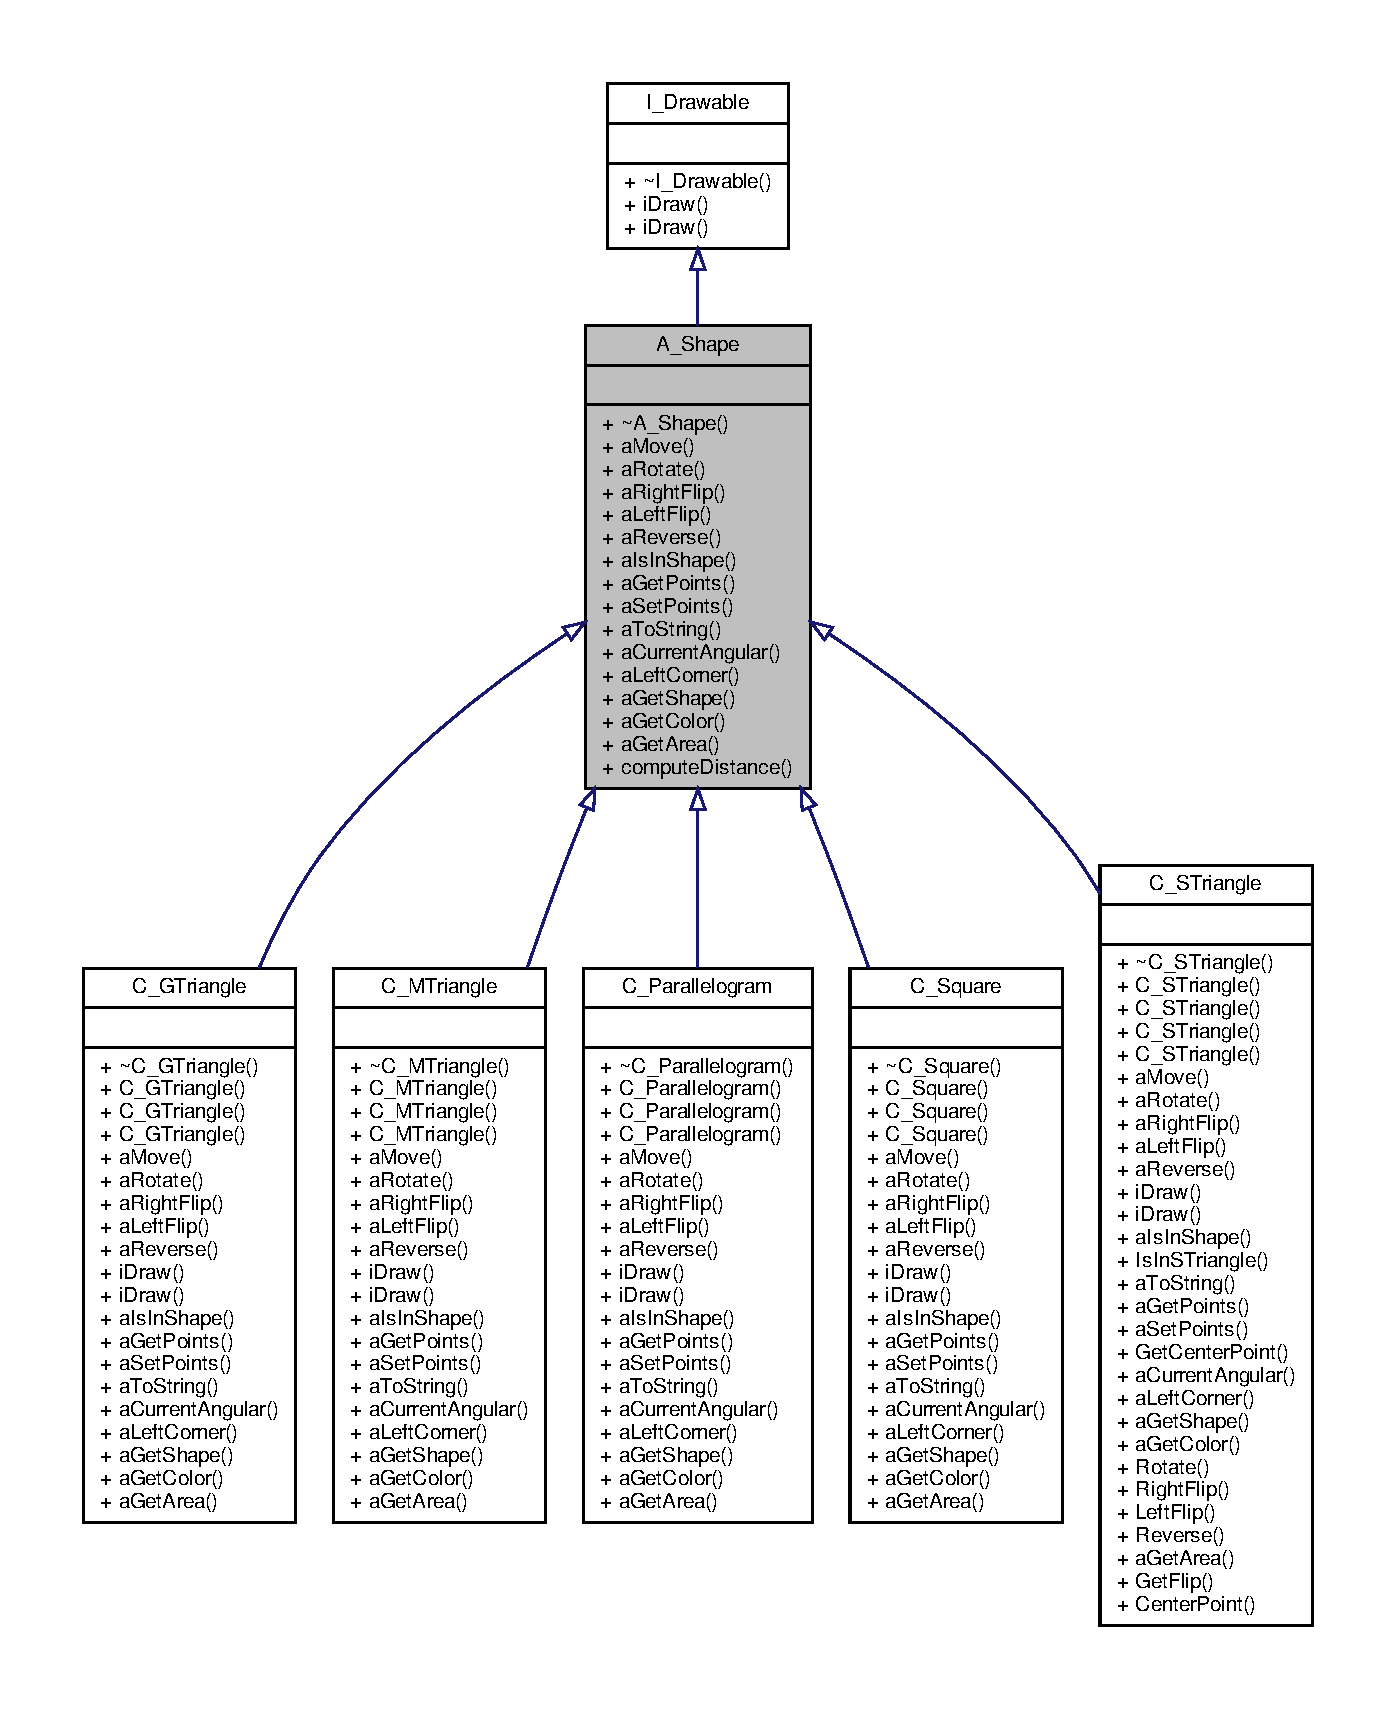
\includegraphics[width=350pt]{classA__Shape__inherit__graph}
\end{center}
\end{figure}


Collaboration diagram for A\+\_\+\+Shape\+:\nopagebreak
\begin{figure}[H]
\begin{center}
\leavevmode
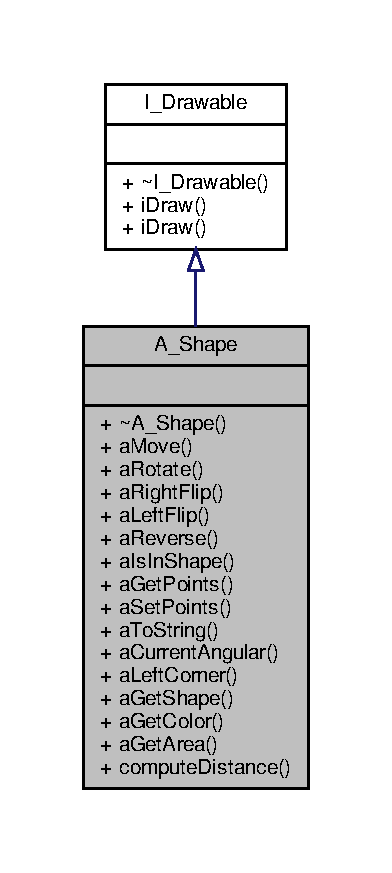
\includegraphics[width=198pt]{classA__Shape__coll__graph}
\end{center}
\end{figure}
\subsection*{Public Member Functions}
\begin{DoxyCompactItemize}
\item 
virtual \hyperlink{classA__Shape_ad0a3bcb28f3d4f42043ea8c592bb5f1f}{$\sim$\+A\+\_\+\+Shape} ()=0
\begin{DoxyCompactList}\small\item\em Destructor of Abstract \hyperlink{classA__Shape}{A\+\_\+\+Shape}. \end{DoxyCompactList}\item 
virtual void \hyperlink{classA__Shape_ab284298db1b557ccfa7ba6de7a5fee2c}{a\+Move} (const \hyperlink{classT__Point}{T\+\_\+\+Point}$<$ double $>$ \&translation)=0
\begin{DoxyCompactList}\small\item\em Pure virtual function. Move the \hyperlink{classA__Shape}{A\+\_\+\+Shape} by point translation. \end{DoxyCompactList}\item 
virtual void \hyperlink{classA__Shape_a25b4e0c34cdb46da5382fe9c7467efaf}{a\+Rotate} (double angular)=0
\begin{DoxyCompactList}\small\item\em Pure virtual function. Rotate the \hyperlink{classA__Shape}{A\+\_\+\+Shape} with specified angular. \end{DoxyCompactList}\item 
virtual void \hyperlink{classA__Shape_a892688cbbad3297e00e87cce0dbfc76d}{a\+Right\+Flip} ()=0
\begin{DoxyCompactList}\small\item\em Pure virtual function. Flip the figure as 45° clock (Pi/4) \end{DoxyCompactList}\item 
virtual void \hyperlink{classA__Shape_abe947e7003cb63be2b4f6c439533427d}{a\+Left\+Flip} ()=0
\begin{DoxyCompactList}\small\item\em Pure virtual function. Flip the figure as 45° anti clock (Pi/4) \end{DoxyCompactList}\item 
virtual void \hyperlink{classA__Shape_afe2c7969d647f6358da13879a7534ecb}{a\+Reverse} ()=0
\begin{DoxyCompactList}\small\item\em Pure virtual function. Reverse the shape as symmetry. \end{DoxyCompactList}\item 
virtual bool \hyperlink{classA__Shape_a63f825cbc9780208d9a137f5c14917d0}{a\+Is\+In\+Shape} (const \hyperlink{classT__Point}{T\+\_\+\+Point}$<$ double $>$ \&point)=0
\begin{DoxyCompactList}\small\item\em Pure virtual function. Check if a point is in this shape. \end{DoxyCompactList}\item 
virtual std\+::vector$<$ \hyperlink{classT__Point}{T\+\_\+\+Point}$<$ double $>$ $>$ \hyperlink{classA__Shape_a9fd1285bd63b1fc88943c9969bf01a5c}{a\+Get\+Points} ()=0
\begin{DoxyCompactList}\small\item\em Pure virtual function. Get all m\+Points of this shape. \end{DoxyCompactList}\item 
virtual bool \hyperlink{classA__Shape_a6996f454b337f8425ad13cba3f7a7c35}{a\+Set\+Points} (const \hyperlink{classT__Point}{T\+\_\+\+Point}$<$ double $>$ \&ref, const \hyperlink{classT__Point}{T\+\_\+\+Point}$<$ double $>$ \&changed)=0
\begin{DoxyCompactList}\small\item\em Pure virtual function. Get all m\+Points of this shape. \end{DoxyCompactList}\item 
virtual std\+::string \hyperlink{classA__Shape_ad8804b4e74543db374af6892367b7c2e}{a\+To\+String} ()=0
\begin{DoxyCompactList}\small\item\em Pure virtual function. Convert all data of \hyperlink{classA__Shape}{A\+\_\+\+Shape} in a string. \end{DoxyCompactList}\item 
virtual double \hyperlink{classA__Shape_a80fa4e009c875dd0ba7fc5bfeeb43f98}{a\+Current\+Angular} ()=0
\begin{DoxyCompactList}\small\item\em Pure virtual function. Get the current angular of a \hyperlink{classA__Shape}{A\+\_\+\+Shape}. \end{DoxyCompactList}\item 
virtual \hyperlink{classT__Point}{T\+\_\+\+Point}$<$ double $>$ \hyperlink{classA__Shape_abe6781b13037bf7ecea8ff9456b31533}{a\+Left\+Corner} ()=0
\begin{DoxyCompactList}\small\item\em Pure virtual function. Take the point at left top corner of a \hyperlink{classA__Shape}{A\+\_\+\+Shape}. \end{DoxyCompactList}\item 
virtual std\+::string \hyperlink{classA__Shape_a1b202256a4e5dcb0edab4ab93a37122c}{a\+Get\+Shape} ()=0
\begin{DoxyCompactList}\small\item\em Pure virtual function. Get the \hyperlink{classA__Shape}{A\+\_\+\+Shape} type. \end{DoxyCompactList}\item 
virtual M\+L\+V\+\_\+\+Color \hyperlink{classA__Shape_a1e90c8132d33e4ac84d42f72606193b2}{a\+Get\+Color} ()=0
\begin{DoxyCompactList}\small\item\em Pure virtual function. Get the color of a \hyperlink{classA__Shape}{A\+\_\+\+Shape}. \end{DoxyCompactList}\item 
virtual double \hyperlink{classA__Shape_a1b142ee2d873d6c217f65de1632e7b6e}{a\+Get\+Area} ()=0
\begin{DoxyCompactList}\small\item\em Pure virtual function. Get the area of a \hyperlink{classA__Shape}{A\+\_\+\+Shape}. \end{DoxyCompactList}\item 
virtual bool \hyperlink{classA__Shape_a24991f7667367b646cae75f60df22e28}{a\+Get\+Status\+Reverse} () const =0
\begin{DoxyCompactList}\small\item\em Get the status of shape reversed or not. \end{DoxyCompactList}\end{DoxyCompactItemize}
\subsection*{Static Public Member Functions}
\begin{DoxyCompactItemize}
\item 
static double \hyperlink{classA__Shape_a2c663e21cf31002323b83f9f98234d33}{compute\+Distance} (const \hyperlink{classT__Point}{T\+\_\+\+Point}$<$ double $>$ \&point1, const \hyperlink{classT__Point}{T\+\_\+\+Point}$<$ double $>$ \&point2)
\begin{DoxyCompactList}\small\item\em Compute distance between 2 m\+Points. \end{DoxyCompactList}\end{DoxyCompactItemize}


\subsection{Detailed Description}
Abstract Class of every \hyperlink{classA__Shape}{A\+\_\+\+Shape}. 

This class manage everything other shape (\hyperlink{classC__STriangle}{C\+\_\+\+S\+Triangle}, \hyperlink{classC__MTriangle}{C\+\_\+\+M\+Triangle}, \hyperlink{classC__GTriangle}{C\+\_\+\+G\+Triangle}, \hyperlink{classC__Square}{C\+\_\+\+Square}, \hyperlink{classC__Parallelogram}{C\+\_\+\+Parallelogram}) 

\subsection{Constructor \& Destructor Documentation}
\mbox{\Hypertarget{classA__Shape_ad0a3bcb28f3d4f42043ea8c592bb5f1f}\label{classA__Shape_ad0a3bcb28f3d4f42043ea8c592bb5f1f}} 
\index{A\+\_\+\+Shape@{A\+\_\+\+Shape}!````~A\+\_\+\+Shape@{$\sim$\+A\+\_\+\+Shape}}
\index{````~A\+\_\+\+Shape@{$\sim$\+A\+\_\+\+Shape}!A\+\_\+\+Shape@{A\+\_\+\+Shape}}
\subsubsection{\texorpdfstring{$\sim$\+A\+\_\+\+Shape()}{~A\_Shape()}}
{\footnotesize\ttfamily A\+\_\+\+Shape\+::$\sim$\+A\+\_\+\+Shape (\begin{DoxyParamCaption}{ }\end{DoxyParamCaption})\hspace{0.3cm}{\ttfamily [pure virtual]}, {\ttfamily [default]}}



Destructor of Abstract \hyperlink{classA__Shape}{A\+\_\+\+Shape}. 



\subsection{Member Function Documentation}
\mbox{\Hypertarget{classA__Shape_a80fa4e009c875dd0ba7fc5bfeeb43f98}\label{classA__Shape_a80fa4e009c875dd0ba7fc5bfeeb43f98}} 
\index{A\+\_\+\+Shape@{A\+\_\+\+Shape}!a\+Current\+Angular@{a\+Current\+Angular}}
\index{a\+Current\+Angular@{a\+Current\+Angular}!A\+\_\+\+Shape@{A\+\_\+\+Shape}}
\subsubsection{\texorpdfstring{a\+Current\+Angular()}{aCurrentAngular()}}
{\footnotesize\ttfamily virtual double A\+\_\+\+Shape\+::a\+Current\+Angular (\begin{DoxyParamCaption}{ }\end{DoxyParamCaption})\hspace{0.3cm}{\ttfamily [pure virtual]}}



Pure virtual function. Get the current angular of a \hyperlink{classA__Shape}{A\+\_\+\+Shape}. 

\begin{DoxyReturn}{Returns}
Return the current angular of a \hyperlink{classA__Shape}{A\+\_\+\+Shape} as double 
\end{DoxyReturn}


Implemented in \hyperlink{classC__STriangle_a38304830925938339c4a4a0ad812e151}{C\+\_\+\+S\+Triangle}, \hyperlink{classC__Parallelogram_a51959da2b0cf083767f39d8065f395f2}{C\+\_\+\+Parallelogram}, \hyperlink{classC__MTriangle_aad1e42f1ec9c486736a403128ba47179}{C\+\_\+\+M\+Triangle}, \hyperlink{classC__Square_ac7779503b305fda4147b735622c66f81}{C\+\_\+\+Square}, and \hyperlink{classC__GTriangle_a98866648972bb78707c61aa7ebc22fb9}{C\+\_\+\+G\+Triangle}.

\mbox{\Hypertarget{classA__Shape_a1b142ee2d873d6c217f65de1632e7b6e}\label{classA__Shape_a1b142ee2d873d6c217f65de1632e7b6e}} 
\index{A\+\_\+\+Shape@{A\+\_\+\+Shape}!a\+Get\+Area@{a\+Get\+Area}}
\index{a\+Get\+Area@{a\+Get\+Area}!A\+\_\+\+Shape@{A\+\_\+\+Shape}}
\subsubsection{\texorpdfstring{a\+Get\+Area()}{aGetArea()}}
{\footnotesize\ttfamily virtual double A\+\_\+\+Shape\+::a\+Get\+Area (\begin{DoxyParamCaption}{ }\end{DoxyParamCaption})\hspace{0.3cm}{\ttfamily [pure virtual]}}



Pure virtual function. Get the area of a \hyperlink{classA__Shape}{A\+\_\+\+Shape}. 

\begin{DoxyReturn}{Returns}
Return the area of a \hyperlink{classA__Shape}{A\+\_\+\+Shape} 
\end{DoxyReturn}


Implemented in \hyperlink{classC__STriangle_aaff25f3c7f7640c3e7c735a77800e96e}{C\+\_\+\+S\+Triangle}, \hyperlink{classC__Parallelogram_a72b4509a33ee27331e5b9bdc8a3278e8}{C\+\_\+\+Parallelogram}, \hyperlink{classC__MTriangle_a1baff5085fc1b9822987e3fc307550ce}{C\+\_\+\+M\+Triangle}, \hyperlink{classC__Square_affd2be59872618d5d1955be360fb73e6}{C\+\_\+\+Square}, and \hyperlink{classC__GTriangle_a4d1c9a050aef86a7eab973b1fe668544}{C\+\_\+\+G\+Triangle}.

\mbox{\Hypertarget{classA__Shape_a1e90c8132d33e4ac84d42f72606193b2}\label{classA__Shape_a1e90c8132d33e4ac84d42f72606193b2}} 
\index{A\+\_\+\+Shape@{A\+\_\+\+Shape}!a\+Get\+Color@{a\+Get\+Color}}
\index{a\+Get\+Color@{a\+Get\+Color}!A\+\_\+\+Shape@{A\+\_\+\+Shape}}
\subsubsection{\texorpdfstring{a\+Get\+Color()}{aGetColor()}}
{\footnotesize\ttfamily virtual M\+L\+V\+\_\+\+Color A\+\_\+\+Shape\+::a\+Get\+Color (\begin{DoxyParamCaption}{ }\end{DoxyParamCaption})\hspace{0.3cm}{\ttfamily [pure virtual]}}



Pure virtual function. Get the color of a \hyperlink{classA__Shape}{A\+\_\+\+Shape}. 

\begin{DoxyReturn}{Returns}
Return the M\+L\+V\+\_\+\+Color of a \hyperlink{classA__Shape}{A\+\_\+\+Shape} 
\end{DoxyReturn}


Implemented in \hyperlink{classC__STriangle_a1a0c315653ece65118705648d09336dd}{C\+\_\+\+S\+Triangle}, \hyperlink{classC__Parallelogram_afd5055e948fcd992be3cdd227c8b4bfb}{C\+\_\+\+Parallelogram}, \hyperlink{classC__MTriangle_aa567d77ce0e6d664beb6eea9268b1bc3}{C\+\_\+\+M\+Triangle}, \hyperlink{classC__Square_a44b1e58b20cc98edc774a73742fec9a7}{C\+\_\+\+Square}, and \hyperlink{classC__GTriangle_a19100d603f9239fd66f1115c4358f0fc}{C\+\_\+\+G\+Triangle}.

\mbox{\Hypertarget{classA__Shape_a9fd1285bd63b1fc88943c9969bf01a5c}\label{classA__Shape_a9fd1285bd63b1fc88943c9969bf01a5c}} 
\index{A\+\_\+\+Shape@{A\+\_\+\+Shape}!a\+Get\+Points@{a\+Get\+Points}}
\index{a\+Get\+Points@{a\+Get\+Points}!A\+\_\+\+Shape@{A\+\_\+\+Shape}}
\subsubsection{\texorpdfstring{a\+Get\+Points()}{aGetPoints()}}
{\footnotesize\ttfamily virtual std\+::vector$<$\hyperlink{classT__Point}{T\+\_\+\+Point}$<$double$>$ $>$ A\+\_\+\+Shape\+::a\+Get\+Points (\begin{DoxyParamCaption}{ }\end{DoxyParamCaption})\hspace{0.3cm}{\ttfamily [pure virtual]}}



Pure virtual function. Get all m\+Points of this shape. 

\begin{DoxyReturn}{Returns}
Return a vector of m\+Points of this shape 
\end{DoxyReturn}


Implemented in \hyperlink{classC__STriangle_a8d144f4451fe2e5bf6f333d8c37f0f57}{C\+\_\+\+S\+Triangle}, \hyperlink{classC__Parallelogram_ae75f316315134020e8423feff917828e}{C\+\_\+\+Parallelogram}, \hyperlink{classC__MTriangle_ada409f8f1015cf7bf9f9ab8fb11da94b}{C\+\_\+\+M\+Triangle}, \hyperlink{classC__Square_aca738fec39149ed697f3d2413cd7cec2}{C\+\_\+\+Square}, and \hyperlink{classC__GTriangle_af3c514a6f5516c297374004a94788877}{C\+\_\+\+G\+Triangle}.

\mbox{\Hypertarget{classA__Shape_a1b202256a4e5dcb0edab4ab93a37122c}\label{classA__Shape_a1b202256a4e5dcb0edab4ab93a37122c}} 
\index{A\+\_\+\+Shape@{A\+\_\+\+Shape}!a\+Get\+Shape@{a\+Get\+Shape}}
\index{a\+Get\+Shape@{a\+Get\+Shape}!A\+\_\+\+Shape@{A\+\_\+\+Shape}}
\subsubsection{\texorpdfstring{a\+Get\+Shape()}{aGetShape()}}
{\footnotesize\ttfamily virtual std\+::string A\+\_\+\+Shape\+::a\+Get\+Shape (\begin{DoxyParamCaption}{ }\end{DoxyParamCaption})\hspace{0.3cm}{\ttfamily [pure virtual]}}



Pure virtual function. Get the \hyperlink{classA__Shape}{A\+\_\+\+Shape} type. 

\begin{DoxyReturn}{Returns}
Return as string a \hyperlink{classA__Shape}{A\+\_\+\+Shape} type 
\end{DoxyReturn}


Implemented in \hyperlink{classC__STriangle_a40c1434870b99112c4457819c9295483}{C\+\_\+\+S\+Triangle}, \hyperlink{classC__Parallelogram_a373fdd3ebdfeffcaa0a72ff7001af8ec}{C\+\_\+\+Parallelogram}, \hyperlink{classC__MTriangle_aca7e38c6bf9695aacf54aa03ecfba978}{C\+\_\+\+M\+Triangle}, \hyperlink{classC__Square_a4919017d3750c1b8deb5f07d22069636}{C\+\_\+\+Square}, and \hyperlink{classC__GTriangle_a039e79bb17dae01997b11243de457d98}{C\+\_\+\+G\+Triangle}.

\mbox{\Hypertarget{classA__Shape_a24991f7667367b646cae75f60df22e28}\label{classA__Shape_a24991f7667367b646cae75f60df22e28}} 
\index{A\+\_\+\+Shape@{A\+\_\+\+Shape}!a\+Get\+Status\+Reverse@{a\+Get\+Status\+Reverse}}
\index{a\+Get\+Status\+Reverse@{a\+Get\+Status\+Reverse}!A\+\_\+\+Shape@{A\+\_\+\+Shape}}
\subsubsection{\texorpdfstring{a\+Get\+Status\+Reverse()}{aGetStatusReverse()}}
{\footnotesize\ttfamily virtual bool A\+\_\+\+Shape\+::a\+Get\+Status\+Reverse (\begin{DoxyParamCaption}{ }\end{DoxyParamCaption}) const\hspace{0.3cm}{\ttfamily [pure virtual]}}



Get the status of shape reversed or not. 

\begin{DoxyReturn}{Returns}
Return true if the shape got reversed, false otherwise 
\end{DoxyReturn}


Implemented in \hyperlink{classC__STriangle_a707d24ede0b9db731dbefee9ab5c017b}{C\+\_\+\+S\+Triangle}, \hyperlink{classC__Parallelogram_a14b00a011ff4fe3170c5ab11af628252}{C\+\_\+\+Parallelogram}, \hyperlink{classC__MTriangle_a5c0488c23e9e64750bb879d0394830b2}{C\+\_\+\+M\+Triangle}, \hyperlink{classC__Square_afe17127df3b112178973ad2182fe9204}{C\+\_\+\+Square}, and \hyperlink{classC__GTriangle_a8aa6444f3d7f001f61cd3903a46f4b67}{C\+\_\+\+G\+Triangle}.

\mbox{\Hypertarget{classA__Shape_a63f825cbc9780208d9a137f5c14917d0}\label{classA__Shape_a63f825cbc9780208d9a137f5c14917d0}} 
\index{A\+\_\+\+Shape@{A\+\_\+\+Shape}!a\+Is\+In\+Shape@{a\+Is\+In\+Shape}}
\index{a\+Is\+In\+Shape@{a\+Is\+In\+Shape}!A\+\_\+\+Shape@{A\+\_\+\+Shape}}
\subsubsection{\texorpdfstring{a\+Is\+In\+Shape()}{aIsInShape()}}
{\footnotesize\ttfamily virtual bool A\+\_\+\+Shape\+::a\+Is\+In\+Shape (\begin{DoxyParamCaption}\item[{const \hyperlink{classT__Point}{T\+\_\+\+Point}$<$ double $>$ \&}]{point }\end{DoxyParamCaption})\hspace{0.3cm}{\ttfamily [pure virtual]}}



Pure virtual function. Check if a point is in this shape. 


\begin{DoxyParams}{Parameters}
{\em point} & \+: \hyperlink{classT__Point}{T\+\_\+\+Point} to check \\
\hline
\end{DoxyParams}
\begin{DoxyReturn}{Returns}
true if Click is in this shape, false if not 
\end{DoxyReturn}


Implemented in \hyperlink{classC__STriangle_a3bc82d7ea53a6a058b9fb49bbd89282c}{C\+\_\+\+S\+Triangle}, \hyperlink{classC__Parallelogram_a9ccee396c30606bfe64df416c22586d5}{C\+\_\+\+Parallelogram}, \hyperlink{classC__MTriangle_ae29e4f6608a0079507c6397b3dbef246}{C\+\_\+\+M\+Triangle}, \hyperlink{classC__Square_ac5ffad4afca051f117b43012fb4dc239}{C\+\_\+\+Square}, and \hyperlink{classC__GTriangle_a417b28c74dd35f81a19b5bd1d214ba8d}{C\+\_\+\+G\+Triangle}.

\mbox{\Hypertarget{classA__Shape_abe6781b13037bf7ecea8ff9456b31533}\label{classA__Shape_abe6781b13037bf7ecea8ff9456b31533}} 
\index{A\+\_\+\+Shape@{A\+\_\+\+Shape}!a\+Left\+Corner@{a\+Left\+Corner}}
\index{a\+Left\+Corner@{a\+Left\+Corner}!A\+\_\+\+Shape@{A\+\_\+\+Shape}}
\subsubsection{\texorpdfstring{a\+Left\+Corner()}{aLeftCorner()}}
{\footnotesize\ttfamily virtual \hyperlink{classT__Point}{T\+\_\+\+Point}$<$double$>$ A\+\_\+\+Shape\+::a\+Left\+Corner (\begin{DoxyParamCaption}{ }\end{DoxyParamCaption})\hspace{0.3cm}{\ttfamily [pure virtual]}}



Pure virtual function. Take the point at left top corner of a \hyperlink{classA__Shape}{A\+\_\+\+Shape}. 

\begin{DoxyReturn}{Returns}
Return the point at left top corner 
\end{DoxyReturn}


Implemented in \hyperlink{classC__STriangle_a8e580f80693ea6f66cca3782ced8e301}{C\+\_\+\+S\+Triangle}, \hyperlink{classC__Parallelogram_a260c557810c63dd97f2dd64bc15b9dc8}{C\+\_\+\+Parallelogram}, \hyperlink{classC__MTriangle_ad077fce026711bf0a25fc4c1cb83ecb9}{C\+\_\+\+M\+Triangle}, \hyperlink{classC__Square_a13e97bb379f1678636e3baf781c2a01b}{C\+\_\+\+Square}, and \hyperlink{classC__GTriangle_a57943afaad0f6b7c3c13aa35a233e93b}{C\+\_\+\+G\+Triangle}.

\mbox{\Hypertarget{classA__Shape_abe947e7003cb63be2b4f6c439533427d}\label{classA__Shape_abe947e7003cb63be2b4f6c439533427d}} 
\index{A\+\_\+\+Shape@{A\+\_\+\+Shape}!a\+Left\+Flip@{a\+Left\+Flip}}
\index{a\+Left\+Flip@{a\+Left\+Flip}!A\+\_\+\+Shape@{A\+\_\+\+Shape}}
\subsubsection{\texorpdfstring{a\+Left\+Flip()}{aLeftFlip()}}
{\footnotesize\ttfamily virtual void A\+\_\+\+Shape\+::a\+Left\+Flip (\begin{DoxyParamCaption}{ }\end{DoxyParamCaption})\hspace{0.3cm}{\ttfamily [pure virtual]}}



Pure virtual function. Flip the figure as 45° anti clock (Pi/4) 



Implemented in \hyperlink{classC__STriangle_aff480b9ec706ee5ae58f6f78318e2728}{C\+\_\+\+S\+Triangle}, \hyperlink{classC__Parallelogram_a284a59c9f1c778ac8da80efedc313354}{C\+\_\+\+Parallelogram}, \hyperlink{classC__MTriangle_a3dcac8e1341a79139577deb851a6481e}{C\+\_\+\+M\+Triangle}, \hyperlink{classC__Square_a31d31862502f0ed24e8331af30100338}{C\+\_\+\+Square}, and \hyperlink{classC__GTriangle_a9ffdddb586b42757ffca6a9ca0c20934}{C\+\_\+\+G\+Triangle}.

\mbox{\Hypertarget{classA__Shape_ab284298db1b557ccfa7ba6de7a5fee2c}\label{classA__Shape_ab284298db1b557ccfa7ba6de7a5fee2c}} 
\index{A\+\_\+\+Shape@{A\+\_\+\+Shape}!a\+Move@{a\+Move}}
\index{a\+Move@{a\+Move}!A\+\_\+\+Shape@{A\+\_\+\+Shape}}
\subsubsection{\texorpdfstring{a\+Move()}{aMove()}}
{\footnotesize\ttfamily virtual void A\+\_\+\+Shape\+::a\+Move (\begin{DoxyParamCaption}\item[{const \hyperlink{classT__Point}{T\+\_\+\+Point}$<$ double $>$ \&}]{translation }\end{DoxyParamCaption})\hspace{0.3cm}{\ttfamily [pure virtual]}}



Pure virtual function. Move the \hyperlink{classA__Shape}{A\+\_\+\+Shape} by point translation. 


\begin{DoxyParams}{Parameters}
{\em translation} & \+: Every m\+Points of this shape will be translate by this \+\_\+\+\_\+\+Parameter \\
\hline
\end{DoxyParams}


Implemented in \hyperlink{classC__STriangle_a82a3c3a847ca6c2d5922921150fa50b5}{C\+\_\+\+S\+Triangle}, \hyperlink{classC__Parallelogram_ac77ea776b24c551114d84eaf147f6977}{C\+\_\+\+Parallelogram}, \hyperlink{classC__MTriangle_a4e185345e7e1ffd5c0b7f1f8dfdbdc59}{C\+\_\+\+M\+Triangle}, \hyperlink{classC__Square_a6727523558c58dcd240ec080f254e7c9}{C\+\_\+\+Square}, and \hyperlink{classC__GTriangle_a07789441ce75f81fd4c4649a0115edbe}{C\+\_\+\+G\+Triangle}.

\mbox{\Hypertarget{classA__Shape_afe2c7969d647f6358da13879a7534ecb}\label{classA__Shape_afe2c7969d647f6358da13879a7534ecb}} 
\index{A\+\_\+\+Shape@{A\+\_\+\+Shape}!a\+Reverse@{a\+Reverse}}
\index{a\+Reverse@{a\+Reverse}!A\+\_\+\+Shape@{A\+\_\+\+Shape}}
\subsubsection{\texorpdfstring{a\+Reverse()}{aReverse()}}
{\footnotesize\ttfamily virtual void A\+\_\+\+Shape\+::a\+Reverse (\begin{DoxyParamCaption}{ }\end{DoxyParamCaption})\hspace{0.3cm}{\ttfamily [pure virtual]}}



Pure virtual function. Reverse the shape as symmetry. 



Implemented in \hyperlink{classC__STriangle_a5402899ec4ea0de3ca3e7aa6f184a1c7}{C\+\_\+\+S\+Triangle}, \hyperlink{classC__Parallelogram_a573447294989d53fadf3d7adfb0640c6}{C\+\_\+\+Parallelogram}, \hyperlink{classC__MTriangle_a44614f4abb94f1a5f963cfb3e8fce7a5}{C\+\_\+\+M\+Triangle}, \hyperlink{classC__Square_a961d1f5c49a45459668744d459863bd2}{C\+\_\+\+Square}, and \hyperlink{classC__GTriangle_a479646fa1265aaf2299b59787c394a27}{C\+\_\+\+G\+Triangle}.

\mbox{\Hypertarget{classA__Shape_a892688cbbad3297e00e87cce0dbfc76d}\label{classA__Shape_a892688cbbad3297e00e87cce0dbfc76d}} 
\index{A\+\_\+\+Shape@{A\+\_\+\+Shape}!a\+Right\+Flip@{a\+Right\+Flip}}
\index{a\+Right\+Flip@{a\+Right\+Flip}!A\+\_\+\+Shape@{A\+\_\+\+Shape}}
\subsubsection{\texorpdfstring{a\+Right\+Flip()}{aRightFlip()}}
{\footnotesize\ttfamily virtual void A\+\_\+\+Shape\+::a\+Right\+Flip (\begin{DoxyParamCaption}{ }\end{DoxyParamCaption})\hspace{0.3cm}{\ttfamily [pure virtual]}}



Pure virtual function. Flip the figure as 45° clock (Pi/4) 



Implemented in \hyperlink{classC__STriangle_aa3cad7b7367c253000cf0f91f55ba600}{C\+\_\+\+S\+Triangle}, \hyperlink{classC__Parallelogram_ab638d55c999ea10da7b5000fd034fbc1}{C\+\_\+\+Parallelogram}, \hyperlink{classC__MTriangle_aa3a1fc0604fa7e13b6c89d242357a163}{C\+\_\+\+M\+Triangle}, \hyperlink{classC__Square_a0ea2df0d283ee4ffa911163e55a0a637}{C\+\_\+\+Square}, and \hyperlink{classC__GTriangle_aa4f808a02ae18bd36c205a5d70eb3fef}{C\+\_\+\+G\+Triangle}.

\mbox{\Hypertarget{classA__Shape_a25b4e0c34cdb46da5382fe9c7467efaf}\label{classA__Shape_a25b4e0c34cdb46da5382fe9c7467efaf}} 
\index{A\+\_\+\+Shape@{A\+\_\+\+Shape}!a\+Rotate@{a\+Rotate}}
\index{a\+Rotate@{a\+Rotate}!A\+\_\+\+Shape@{A\+\_\+\+Shape}}
\subsubsection{\texorpdfstring{a\+Rotate()}{aRotate()}}
{\footnotesize\ttfamily virtual void A\+\_\+\+Shape\+::a\+Rotate (\begin{DoxyParamCaption}\item[{double}]{angular }\end{DoxyParamCaption})\hspace{0.3cm}{\ttfamily [pure virtual]}}



Pure virtual function. Rotate the \hyperlink{classA__Shape}{A\+\_\+\+Shape} with specified angular. 


\begin{DoxyParams}{Parameters}
{\em angular} & \+: This angular should be between (0, 2\+PI) \\
\hline
\end{DoxyParams}


Implemented in \hyperlink{classC__STriangle_a52612242aba17043862355c030637a18}{C\+\_\+\+S\+Triangle}, \hyperlink{classC__Parallelogram_a07b6dfae7100a409cdcf04d710ac9c3f}{C\+\_\+\+Parallelogram}, \hyperlink{classC__MTriangle_a33aa36879be70b0a11863801da56e92e}{C\+\_\+\+M\+Triangle}, \hyperlink{classC__Square_af74175a5e8d61216d68fde18ef9c9481}{C\+\_\+\+Square}, and \hyperlink{classC__GTriangle_a29c641aea4ef5fa4224b42dffc5fefa5}{C\+\_\+\+G\+Triangle}.

\mbox{\Hypertarget{classA__Shape_a6996f454b337f8425ad13cba3f7a7c35}\label{classA__Shape_a6996f454b337f8425ad13cba3f7a7c35}} 
\index{A\+\_\+\+Shape@{A\+\_\+\+Shape}!a\+Set\+Points@{a\+Set\+Points}}
\index{a\+Set\+Points@{a\+Set\+Points}!A\+\_\+\+Shape@{A\+\_\+\+Shape}}
\subsubsection{\texorpdfstring{a\+Set\+Points()}{aSetPoints()}}
{\footnotesize\ttfamily virtual bool A\+\_\+\+Shape\+::a\+Set\+Points (\begin{DoxyParamCaption}\item[{const \hyperlink{classT__Point}{T\+\_\+\+Point}$<$ double $>$ \&}]{ref,  }\item[{const \hyperlink{classT__Point}{T\+\_\+\+Point}$<$ double $>$ \&}]{changed }\end{DoxyParamCaption})\hspace{0.3cm}{\ttfamily [pure virtual]}}



Pure virtual function. Get all m\+Points of this shape. 

\begin{DoxyReturn}{Returns}
Return a vector of m\+Points of this shape 
\end{DoxyReturn}


Implemented in \hyperlink{classC__STriangle_a431802d5e10b69f535e7929a23963b5e}{C\+\_\+\+S\+Triangle}, \hyperlink{classC__Parallelogram_adfe1c40f2d33955617e3a535c548dfa0}{C\+\_\+\+Parallelogram}, \hyperlink{classC__MTriangle_a5a3971eb0aafc16e5a34bd94130d7c6b}{C\+\_\+\+M\+Triangle}, \hyperlink{classC__Square_a295a170686422b745587a250ebe08a5e}{C\+\_\+\+Square}, and \hyperlink{classC__GTriangle_a18c134ddf90bc4f5729064a47094068b}{C\+\_\+\+G\+Triangle}.

\mbox{\Hypertarget{classA__Shape_ad8804b4e74543db374af6892367b7c2e}\label{classA__Shape_ad8804b4e74543db374af6892367b7c2e}} 
\index{A\+\_\+\+Shape@{A\+\_\+\+Shape}!a\+To\+String@{a\+To\+String}}
\index{a\+To\+String@{a\+To\+String}!A\+\_\+\+Shape@{A\+\_\+\+Shape}}
\subsubsection{\texorpdfstring{a\+To\+String()}{aToString()}}
{\footnotesize\ttfamily virtual std\+::string A\+\_\+\+Shape\+::a\+To\+String (\begin{DoxyParamCaption}{ }\end{DoxyParamCaption})\hspace{0.3cm}{\ttfamily [pure virtual]}}



Pure virtual function. Convert all data of \hyperlink{classA__Shape}{A\+\_\+\+Shape} in a string. 

\begin{DoxyReturn}{Returns}
Return a string which contains every m\+Points of this shape 
\end{DoxyReturn}


Implemented in \hyperlink{classC__STriangle_a1ea089f6a82c2770e0529c4a9fc07d90}{C\+\_\+\+S\+Triangle}, \hyperlink{classC__Parallelogram_add67ef2aba5e14c27e30a958e4843223}{C\+\_\+\+Parallelogram}, \hyperlink{classC__MTriangle_a3a769eb21278ec456292d88385b332a2}{C\+\_\+\+M\+Triangle}, \hyperlink{classC__Square_ab2cada51b25cd35b9a79e461767e56f0}{C\+\_\+\+Square}, and \hyperlink{classC__GTriangle_aa432e8b8320db8a53ef1d59b486ed7ce}{C\+\_\+\+G\+Triangle}.

\mbox{\Hypertarget{classA__Shape_a2c663e21cf31002323b83f9f98234d33}\label{classA__Shape_a2c663e21cf31002323b83f9f98234d33}} 
\index{A\+\_\+\+Shape@{A\+\_\+\+Shape}!compute\+Distance@{compute\+Distance}}
\index{compute\+Distance@{compute\+Distance}!A\+\_\+\+Shape@{A\+\_\+\+Shape}}
\subsubsection{\texorpdfstring{compute\+Distance()}{computeDistance()}}
{\footnotesize\ttfamily static double A\+\_\+\+Shape\+::compute\+Distance (\begin{DoxyParamCaption}\item[{const \hyperlink{classT__Point}{T\+\_\+\+Point}$<$ double $>$ \&}]{point1,  }\item[{const \hyperlink{classT__Point}{T\+\_\+\+Point}$<$ double $>$ \&}]{point2 }\end{DoxyParamCaption})\hspace{0.3cm}{\ttfamily [inline]}, {\ttfamily [static]}}



Compute distance between 2 m\+Points. 


\begin{DoxyParams}{Parameters}
{\em point1} & \+: First point \\
\hline
{\em point2} & \+: Second point \\
\hline
\end{DoxyParams}
\begin{DoxyReturn}{Returns}
Return the distance between these two m\+Points 
\end{DoxyReturn}


The documentation for this class was generated from the following files\+:\begin{DoxyCompactItemize}
\item 
include/drawable/\hyperlink{A__Shape_8hpp}{A\+\_\+\+Shape.\+hpp}\item 
src/drawable/\hyperlink{A__Shape_8cpp}{A\+\_\+\+Shape.\+cpp}\end{DoxyCompactItemize}

\hypertarget{classC__Button}{}\section{C\+\_\+\+Button Class Reference}
\label{classC__Button}\index{C\+\_\+\+Button@{C\+\_\+\+Button}}


\hyperlink{classC__Button}{C\+\_\+\+Button} of the \hyperlink{classC__Menu}{C\+\_\+\+Menu}.  




{\ttfamily \#include $<$C\+\_\+\+Button.\+hpp$>$}



Collaboration diagram for C\+\_\+\+Button\+:\nopagebreak
\begin{figure}[H]
\begin{center}
\leavevmode
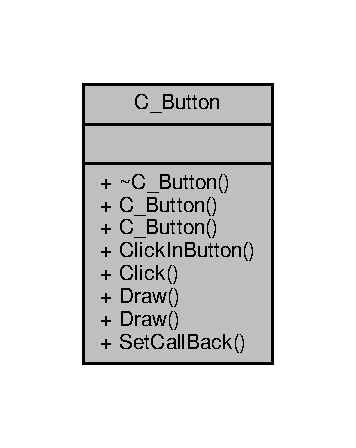
\includegraphics[width=171pt]{classC__Button__coll__graph}
\end{center}
\end{figure}
\subsection*{Public Member Functions}
\begin{DoxyCompactItemize}
\item 
\hyperlink{classC__Button_a8581fb2ad14e232e97040388bdc992e4}{$\sim$\+C\+\_\+\+Button} ()
\begin{DoxyCompactList}\small\item\em Class methods. \end{DoxyCompactList}\item 
\hyperlink{classC__Button_a39291cec8e3a327343328f6fa1a3b3d9}{C\+\_\+\+Button} (const \hyperlink{classT__Point}{T\+\_\+\+Point}$<$ int $>$ \&point, const \hyperlink{classT__Point}{T\+\_\+\+Point}$<$ int $>$ \&sizing, std\+::string text)
\begin{DoxyCompactList}\small\item\em Constructor of a \hyperlink{classC__Button}{C\+\_\+\+Button}. \end{DoxyCompactList}\item 
\hyperlink{classC__Button_aed99ebc9be8ebd50a09c909eb95ec226}{C\+\_\+\+Button} (const \hyperlink{classT__Point}{T\+\_\+\+Point}$<$ int $>$ \&point, const \hyperlink{classT__Point}{T\+\_\+\+Point}$<$ int $>$ \&sizing, std\+::string text, std\+::function$<$ int(int)$>$ callback)
\begin{DoxyCompactList}\small\item\em Constructor of a \hyperlink{classC__Button}{C\+\_\+\+Button}. \end{DoxyCompactList}\item 
bool \hyperlink{classC__Button_a805c797b9afdddb5896a516a3e783882}{Click\+In\+Button} (const \hyperlink{classT__Point}{T\+\_\+\+Point}$<$ int $>$ \&click)
\begin{DoxyCompactList}\small\item\em Check if a Click is in the button. \end{DoxyCompactList}\item 
int \hyperlink{classC__Button_ac743591b5933dd95b571d5956c7d669b}{Click} (int)
\begin{DoxyCompactList}\small\item\em Define a value about a Click. \end{DoxyCompactList}\item 
void \hyperlink{classC__Button_a71f9a7d92a30818af1539104e6b963fb}{Draw} ()
\begin{DoxyCompactList}\small\item\em Draw the button. \end{DoxyCompactList}\item 
void \hyperlink{classC__Button_a6c507d4567ca21676e9980f8cf3d26b5}{Draw} (M\+L\+V\+\_\+\+Color color)
\begin{DoxyCompactList}\small\item\em Draw the button with specific color. \end{DoxyCompactList}\item 
void \hyperlink{classC__Button_aedb01f3229d8176f6a9475cf2edae8f0}{Set\+Call\+Back} (std\+::function$<$ int(int)$>$ callback)
\begin{DoxyCompactList}\small\item\em Set a callback for a button. \end{DoxyCompactList}\item 
\hyperlink{classC__Button_a8581fb2ad14e232e97040388bdc992e4}{$\sim$\+C\+\_\+\+Button} ()
\begin{DoxyCompactList}\small\item\em Class methods. \end{DoxyCompactList}\item 
\hyperlink{classC__Button_a39291cec8e3a327343328f6fa1a3b3d9}{C\+\_\+\+Button} (const \hyperlink{classT__Point}{T\+\_\+\+Point}$<$ int $>$ \&point, const \hyperlink{classT__Point}{T\+\_\+\+Point}$<$ int $>$ \&sizing, std\+::string text)
\begin{DoxyCompactList}\small\item\em Constructor of a \hyperlink{classC__Button}{C\+\_\+\+Button}. \end{DoxyCompactList}\item 
\hyperlink{classC__Button_aed99ebc9be8ebd50a09c909eb95ec226}{C\+\_\+\+Button} (const \hyperlink{classT__Point}{T\+\_\+\+Point}$<$ int $>$ \&point, const \hyperlink{classT__Point}{T\+\_\+\+Point}$<$ int $>$ \&sizing, std\+::string text, std\+::function$<$ int(int)$>$ callback)
\begin{DoxyCompactList}\small\item\em Constructor of a \hyperlink{classC__Button}{C\+\_\+\+Button}. \end{DoxyCompactList}\item 
bool \hyperlink{classC__Button_a805c797b9afdddb5896a516a3e783882}{Click\+In\+Button} (const \hyperlink{classT__Point}{T\+\_\+\+Point}$<$ int $>$ \&click)
\begin{DoxyCompactList}\small\item\em Check if a Click is in the button. \end{DoxyCompactList}\item 
int \hyperlink{classC__Button_ac743591b5933dd95b571d5956c7d669b}{Click} (int)
\begin{DoxyCompactList}\small\item\em Define a value about a Click. \end{DoxyCompactList}\item 
void \hyperlink{classC__Button_a71f9a7d92a30818af1539104e6b963fb}{Draw} ()
\begin{DoxyCompactList}\small\item\em Draw the button. \end{DoxyCompactList}\item 
void \hyperlink{classC__Button_a6c507d4567ca21676e9980f8cf3d26b5}{Draw} (M\+L\+V\+\_\+\+Color color)
\begin{DoxyCompactList}\small\item\em Draw the button with specific color. \end{DoxyCompactList}\item 
void \hyperlink{classC__Button_aedb01f3229d8176f6a9475cf2edae8f0}{Set\+Call\+Back} (std\+::function$<$ int(int)$>$ callback)
\begin{DoxyCompactList}\small\item\em Set a callback for a button. \end{DoxyCompactList}\end{DoxyCompactItemize}


\subsection{Detailed Description}
\hyperlink{classC__Button}{C\+\_\+\+Button} of the \hyperlink{classC__Menu}{C\+\_\+\+Menu}. 

This class manage all m\+Buttons of the menu 

\subsection{Constructor \& Destructor Documentation}
\mbox{\Hypertarget{classC__Button_a8581fb2ad14e232e97040388bdc992e4}\label{classC__Button_a8581fb2ad14e232e97040388bdc992e4}} 
\index{C\+\_\+\+Button@{C\+\_\+\+Button}!````~C\+\_\+\+Button@{$\sim$\+C\+\_\+\+Button}}
\index{````~C\+\_\+\+Button@{$\sim$\+C\+\_\+\+Button}!C\+\_\+\+Button@{C\+\_\+\+Button}}
\subsubsection{\texorpdfstring{$\sim$\+C\+\_\+\+Button()}{~C\_Button()}\hspace{0.1cm}{\footnotesize\ttfamily [1/2]}}
{\footnotesize\ttfamily C\+\_\+\+Button\+::$\sim$\+C\+\_\+\+Button (\begin{DoxyParamCaption}{ }\end{DoxyParamCaption})\hspace{0.3cm}{\ttfamily [default]}}



Class methods. 

Destructor of the \hyperlink{classC__Button}{C\+\_\+\+Button} \mbox{\Hypertarget{classC__Button_a39291cec8e3a327343328f6fa1a3b3d9}\label{classC__Button_a39291cec8e3a327343328f6fa1a3b3d9}} 
\index{C\+\_\+\+Button@{C\+\_\+\+Button}!C\+\_\+\+Button@{C\+\_\+\+Button}}
\index{C\+\_\+\+Button@{C\+\_\+\+Button}!C\+\_\+\+Button@{C\+\_\+\+Button}}
\subsubsection{\texorpdfstring{C\+\_\+\+Button()}{C\_Button()}\hspace{0.1cm}{\footnotesize\ttfamily [1/4]}}
{\footnotesize\ttfamily C\+\_\+\+Button\+::\+C\+\_\+\+Button (\begin{DoxyParamCaption}\item[{const \hyperlink{classT__Point}{T\+\_\+\+Point}$<$ int $>$ \&}]{point,  }\item[{const \hyperlink{classT__Point}{T\+\_\+\+Point}$<$ int $>$ \&}]{sizing,  }\item[{std\+::string}]{text }\end{DoxyParamCaption})}



Constructor of a \hyperlink{classC__Button}{C\+\_\+\+Button}. 


\begin{DoxyParams}{Parameters}
{\em point} & \+: Top left point position of the button \\
\hline
{\em sizing} & \+: Sizing of the button, (width , height) \\
\hline
{\em text} & \+: Text of the button \\
\hline
\end{DoxyParams}
\mbox{\Hypertarget{classC__Button_aed99ebc9be8ebd50a09c909eb95ec226}\label{classC__Button_aed99ebc9be8ebd50a09c909eb95ec226}} 
\index{C\+\_\+\+Button@{C\+\_\+\+Button}!C\+\_\+\+Button@{C\+\_\+\+Button}}
\index{C\+\_\+\+Button@{C\+\_\+\+Button}!C\+\_\+\+Button@{C\+\_\+\+Button}}
\subsubsection{\texorpdfstring{C\+\_\+\+Button()}{C\_Button()}\hspace{0.1cm}{\footnotesize\ttfamily [2/4]}}
{\footnotesize\ttfamily C\+\_\+\+Button\+::\+C\+\_\+\+Button (\begin{DoxyParamCaption}\item[{const \hyperlink{classT__Point}{T\+\_\+\+Point}$<$ int $>$ \&}]{point,  }\item[{const \hyperlink{classT__Point}{T\+\_\+\+Point}$<$ int $>$ \&}]{sizing,  }\item[{std\+::string}]{text,  }\item[{std\+::function$<$ int(int)$>$}]{callback }\end{DoxyParamCaption})}



Constructor of a \hyperlink{classC__Button}{C\+\_\+\+Button}. 


\begin{DoxyParams}{Parameters}
{\em point} & \+: Top left point position of the button \\
\hline
{\em sizing} & \+: Sizing of the button, (width , height) \\
\hline
{\em text} & \+: Text of the button \\
\hline
{\em callback} & \+: Pointer of function for callback \\
\hline
\end{DoxyParams}
\mbox{\Hypertarget{classC__Button_a8581fb2ad14e232e97040388bdc992e4}\label{classC__Button_a8581fb2ad14e232e97040388bdc992e4}} 
\index{C\+\_\+\+Button@{C\+\_\+\+Button}!````~C\+\_\+\+Button@{$\sim$\+C\+\_\+\+Button}}
\index{````~C\+\_\+\+Button@{$\sim$\+C\+\_\+\+Button}!C\+\_\+\+Button@{C\+\_\+\+Button}}
\subsubsection{\texorpdfstring{$\sim$\+C\+\_\+\+Button()}{~C\_Button()}\hspace{0.1cm}{\footnotesize\ttfamily [2/2]}}
{\footnotesize\ttfamily C\+\_\+\+Button\+::$\sim$\+C\+\_\+\+Button (\begin{DoxyParamCaption}{ }\end{DoxyParamCaption})}



Class methods. 

Destructor of the \hyperlink{classC__Button}{C\+\_\+\+Button} \mbox{\Hypertarget{classC__Button_a39291cec8e3a327343328f6fa1a3b3d9}\label{classC__Button_a39291cec8e3a327343328f6fa1a3b3d9}} 
\index{C\+\_\+\+Button@{C\+\_\+\+Button}!C\+\_\+\+Button@{C\+\_\+\+Button}}
\index{C\+\_\+\+Button@{C\+\_\+\+Button}!C\+\_\+\+Button@{C\+\_\+\+Button}}
\subsubsection{\texorpdfstring{C\+\_\+\+Button()}{C\_Button()}\hspace{0.1cm}{\footnotesize\ttfamily [3/4]}}
{\footnotesize\ttfamily C\+\_\+\+Button\+::\+C\+\_\+\+Button (\begin{DoxyParamCaption}\item[{const \hyperlink{classT__Point}{T\+\_\+\+Point}$<$ int $>$ \&}]{point,  }\item[{const \hyperlink{classT__Point}{T\+\_\+\+Point}$<$ int $>$ \&}]{sizing,  }\item[{std\+::string}]{text }\end{DoxyParamCaption})}



Constructor of a \hyperlink{classC__Button}{C\+\_\+\+Button}. 


\begin{DoxyParams}{Parameters}
{\em point} & \+: Top left point position of the button \\
\hline
{\em sizing} & \+: Sizing of the button, (width , height) \\
\hline
{\em text} & \+: Text of the button \\
\hline
\end{DoxyParams}
\mbox{\Hypertarget{classC__Button_aed99ebc9be8ebd50a09c909eb95ec226}\label{classC__Button_aed99ebc9be8ebd50a09c909eb95ec226}} 
\index{C\+\_\+\+Button@{C\+\_\+\+Button}!C\+\_\+\+Button@{C\+\_\+\+Button}}
\index{C\+\_\+\+Button@{C\+\_\+\+Button}!C\+\_\+\+Button@{C\+\_\+\+Button}}
\subsubsection{\texorpdfstring{C\+\_\+\+Button()}{C\_Button()}\hspace{0.1cm}{\footnotesize\ttfamily [4/4]}}
{\footnotesize\ttfamily C\+\_\+\+Button\+::\+C\+\_\+\+Button (\begin{DoxyParamCaption}\item[{const \hyperlink{classT__Point}{T\+\_\+\+Point}$<$ int $>$ \&}]{point,  }\item[{const \hyperlink{classT__Point}{T\+\_\+\+Point}$<$ int $>$ \&}]{sizing,  }\item[{std\+::string}]{text,  }\item[{std\+::function$<$ int(int)$>$}]{callback }\end{DoxyParamCaption})}



Constructor of a \hyperlink{classC__Button}{C\+\_\+\+Button}. 


\begin{DoxyParams}{Parameters}
{\em point} & \+: Top left point position of the button \\
\hline
{\em sizing} & \+: Sizing of the button, (width , height) \\
\hline
{\em text} & \+: Text of the button \\
\hline
{\em callback} & \+: Pointer of function for callback \\
\hline
\end{DoxyParams}


\subsection{Member Function Documentation}
\mbox{\Hypertarget{classC__Button_ac743591b5933dd95b571d5956c7d669b}\label{classC__Button_ac743591b5933dd95b571d5956c7d669b}} 
\index{C\+\_\+\+Button@{C\+\_\+\+Button}!Click@{Click}}
\index{Click@{Click}!C\+\_\+\+Button@{C\+\_\+\+Button}}
\subsubsection{\texorpdfstring{Click()}{Click()}\hspace{0.1cm}{\footnotesize\ttfamily [1/2]}}
{\footnotesize\ttfamily int C\+\_\+\+Button\+::\+Click (\begin{DoxyParamCaption}\item[{int}]{val }\end{DoxyParamCaption})}



Define a value about a Click. 

\begin{DoxyReturn}{Returns}
Return a value about a Click 
\end{DoxyReturn}
\mbox{\Hypertarget{classC__Button_ac743591b5933dd95b571d5956c7d669b}\label{classC__Button_ac743591b5933dd95b571d5956c7d669b}} 
\index{C\+\_\+\+Button@{C\+\_\+\+Button}!Click@{Click}}
\index{Click@{Click}!C\+\_\+\+Button@{C\+\_\+\+Button}}
\subsubsection{\texorpdfstring{Click()}{Click()}\hspace{0.1cm}{\footnotesize\ttfamily [2/2]}}
{\footnotesize\ttfamily int C\+\_\+\+Button\+::\+Click (\begin{DoxyParamCaption}\item[{int}]{ }\end{DoxyParamCaption})}



Define a value about a Click. 

\begin{DoxyReturn}{Returns}
Return a value about a Click 
\end{DoxyReturn}
\mbox{\Hypertarget{classC__Button_a805c797b9afdddb5896a516a3e783882}\label{classC__Button_a805c797b9afdddb5896a516a3e783882}} 
\index{C\+\_\+\+Button@{C\+\_\+\+Button}!Click\+In\+Button@{Click\+In\+Button}}
\index{Click\+In\+Button@{Click\+In\+Button}!C\+\_\+\+Button@{C\+\_\+\+Button}}
\subsubsection{\texorpdfstring{Click\+In\+Button()}{ClickInButton()}\hspace{0.1cm}{\footnotesize\ttfamily [1/2]}}
{\footnotesize\ttfamily bool C\+\_\+\+Button\+::\+Click\+In\+Button (\begin{DoxyParamCaption}\item[{const \hyperlink{classT__Point}{T\+\_\+\+Point}$<$ int $>$ \&}]{click }\end{DoxyParamCaption})}



Check if a Click is in the button. 


\begin{DoxyParams}{Parameters}
{\em click} & \+: \hyperlink{classT__Point}{T\+\_\+\+Point} to check \\
\hline
\end{DoxyParams}
\begin{DoxyReturn}{Returns}
True if the Click is in this button, false if not 
\end{DoxyReturn}
\mbox{\Hypertarget{classC__Button_a805c797b9afdddb5896a516a3e783882}\label{classC__Button_a805c797b9afdddb5896a516a3e783882}} 
\index{C\+\_\+\+Button@{C\+\_\+\+Button}!Click\+In\+Button@{Click\+In\+Button}}
\index{Click\+In\+Button@{Click\+In\+Button}!C\+\_\+\+Button@{C\+\_\+\+Button}}
\subsubsection{\texorpdfstring{Click\+In\+Button()}{ClickInButton()}\hspace{0.1cm}{\footnotesize\ttfamily [2/2]}}
{\footnotesize\ttfamily bool C\+\_\+\+Button\+::\+Click\+In\+Button (\begin{DoxyParamCaption}\item[{const \hyperlink{classT__Point}{T\+\_\+\+Point}$<$ int $>$ \&}]{click }\end{DoxyParamCaption})}



Check if a Click is in the button. 


\begin{DoxyParams}{Parameters}
{\em click} & \+: \hyperlink{classT__Point}{T\+\_\+\+Point} to check \\
\hline
\end{DoxyParams}
\begin{DoxyReturn}{Returns}
True if the Click is in this button, false if not 
\end{DoxyReturn}
\mbox{\Hypertarget{classC__Button_a71f9a7d92a30818af1539104e6b963fb}\label{classC__Button_a71f9a7d92a30818af1539104e6b963fb}} 
\index{C\+\_\+\+Button@{C\+\_\+\+Button}!Draw@{Draw}}
\index{Draw@{Draw}!C\+\_\+\+Button@{C\+\_\+\+Button}}
\subsubsection{\texorpdfstring{Draw()}{Draw()}\hspace{0.1cm}{\footnotesize\ttfamily [1/4]}}
{\footnotesize\ttfamily void C\+\_\+\+Button\+::\+Draw (\begin{DoxyParamCaption}{ }\end{DoxyParamCaption})}



Draw the button. 

\mbox{\Hypertarget{classC__Button_a71f9a7d92a30818af1539104e6b963fb}\label{classC__Button_a71f9a7d92a30818af1539104e6b963fb}} 
\index{C\+\_\+\+Button@{C\+\_\+\+Button}!Draw@{Draw}}
\index{Draw@{Draw}!C\+\_\+\+Button@{C\+\_\+\+Button}}
\subsubsection{\texorpdfstring{Draw()}{Draw()}\hspace{0.1cm}{\footnotesize\ttfamily [2/4]}}
{\footnotesize\ttfamily void C\+\_\+\+Button\+::\+Draw (\begin{DoxyParamCaption}{ }\end{DoxyParamCaption})}



Draw the button. 

\mbox{\Hypertarget{classC__Button_a6c507d4567ca21676e9980f8cf3d26b5}\label{classC__Button_a6c507d4567ca21676e9980f8cf3d26b5}} 
\index{C\+\_\+\+Button@{C\+\_\+\+Button}!Draw@{Draw}}
\index{Draw@{Draw}!C\+\_\+\+Button@{C\+\_\+\+Button}}
\subsubsection{\texorpdfstring{Draw()}{Draw()}\hspace{0.1cm}{\footnotesize\ttfamily [3/4]}}
{\footnotesize\ttfamily void C\+\_\+\+Button\+::\+Draw (\begin{DoxyParamCaption}\item[{M\+L\+V\+\_\+\+Color}]{color }\end{DoxyParamCaption})}



Draw the button with specific color. 


\begin{DoxyParams}{Parameters}
{\em color} & \+: M\+L\+V\+\_\+\+Color needed to draw the button \\
\hline
\end{DoxyParams}
\mbox{\Hypertarget{classC__Button_a6c507d4567ca21676e9980f8cf3d26b5}\label{classC__Button_a6c507d4567ca21676e9980f8cf3d26b5}} 
\index{C\+\_\+\+Button@{C\+\_\+\+Button}!Draw@{Draw}}
\index{Draw@{Draw}!C\+\_\+\+Button@{C\+\_\+\+Button}}
\subsubsection{\texorpdfstring{Draw()}{Draw()}\hspace{0.1cm}{\footnotesize\ttfamily [4/4]}}
{\footnotesize\ttfamily void C\+\_\+\+Button\+::\+Draw (\begin{DoxyParamCaption}\item[{M\+L\+V\+\_\+\+Color}]{color }\end{DoxyParamCaption})}



Draw the button with specific color. 


\begin{DoxyParams}{Parameters}
{\em color} & \+: M\+L\+V\+\_\+\+Color needed to draw the button \\
\hline
\end{DoxyParams}
\mbox{\Hypertarget{classC__Button_aedb01f3229d8176f6a9475cf2edae8f0}\label{classC__Button_aedb01f3229d8176f6a9475cf2edae8f0}} 
\index{C\+\_\+\+Button@{C\+\_\+\+Button}!Set\+Call\+Back@{Set\+Call\+Back}}
\index{Set\+Call\+Back@{Set\+Call\+Back}!C\+\_\+\+Button@{C\+\_\+\+Button}}
\subsubsection{\texorpdfstring{Set\+Call\+Back()}{SetCallBack()}\hspace{0.1cm}{\footnotesize\ttfamily [1/2]}}
{\footnotesize\ttfamily void C\+\_\+\+Button\+::\+Set\+Call\+Back (\begin{DoxyParamCaption}\item[{std\+::function$<$ int(int)$>$}]{callback }\end{DoxyParamCaption})}



Set a callback for a button. 


\begin{DoxyParams}{Parameters}
{\em callback} & \+: Requires a pointer of function for set the callback \\
\hline
\end{DoxyParams}
\mbox{\Hypertarget{classC__Button_aedb01f3229d8176f6a9475cf2edae8f0}\label{classC__Button_aedb01f3229d8176f6a9475cf2edae8f0}} 
\index{C\+\_\+\+Button@{C\+\_\+\+Button}!Set\+Call\+Back@{Set\+Call\+Back}}
\index{Set\+Call\+Back@{Set\+Call\+Back}!C\+\_\+\+Button@{C\+\_\+\+Button}}
\subsubsection{\texorpdfstring{Set\+Call\+Back()}{SetCallBack()}\hspace{0.1cm}{\footnotesize\ttfamily [2/2]}}
{\footnotesize\ttfamily void C\+\_\+\+Button\+::\+Set\+Call\+Back (\begin{DoxyParamCaption}\item[{std\+::function$<$ int(int)$>$}]{callback }\end{DoxyParamCaption})}



Set a callback for a button. 


\begin{DoxyParams}{Parameters}
{\em callback} & \+: Requires a pointer of function for set the callback \\
\hline
\end{DoxyParams}


The documentation for this class was generated from the following files\+:\begin{DoxyCompactItemize}
\item 
include/\hyperlink{C__Button_8hpp}{C\+\_\+\+Button.\+hpp}\item 
src/drawable/\hyperlink{C__Button_8cpp}{C\+\_\+\+Button.\+cpp}\end{DoxyCompactItemize}

\hypertarget{classC__Game}{}\section{C\+\_\+\+Game Class Reference}
\label{classC__Game}\index{C\+\_\+\+Game@{C\+\_\+\+Game}}


Class of the main \hyperlink{classC__Game}{C\+\_\+\+Game}.  




{\ttfamily \#include $<$C\+\_\+\+Game.\+hpp$>$}



Collaboration diagram for C\+\_\+\+Game\+:
\nopagebreak
\begin{figure}[H]
\begin{center}
\leavevmode
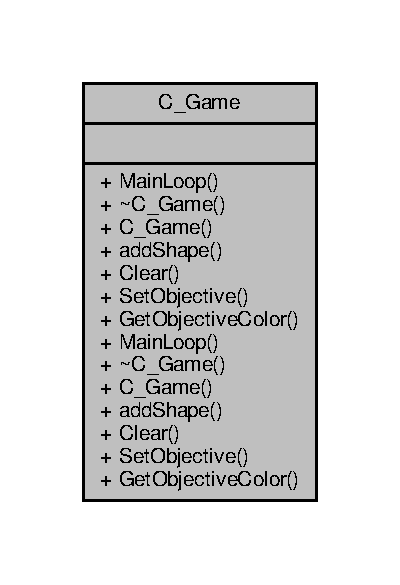
\includegraphics[width=192pt]{classC__Game__coll__graph}
\end{center}
\end{figure}
\subsection*{Public Member Functions}
\begin{DoxyCompactItemize}
\item 
void \hyperlink{classC__Game_aa15149075c2a4bd4704235d83c1c4f20}{Main\+Loop} ()
\begin{DoxyCompactList}\small\item\em Main loop of the game. \end{DoxyCompactList}\item 
\hyperlink{classC__Game_a4a11981e90a66634568f59ac823a697e}{$\sim$\+C\+\_\+\+Game} ()
\begin{DoxyCompactList}\small\item\em Destructor of the game. \end{DoxyCompactList}\item 
\hyperlink{classC__Game_ac5a1aba1deb606a281d3992459566716}{C\+\_\+\+Game} (int w, int h)
\begin{DoxyCompactList}\small\item\em Constructor of the game, initialize a game with an sizing. \end{DoxyCompactList}\item 
void \hyperlink{classC__Game_ad2b7512192879ec7cd76d4eed4fef938}{add\+Shape} (std\+::shared\+\_\+ptr$<$ \hyperlink{classA__Shape}{A\+\_\+\+Shape} $>$ s)
\begin{DoxyCompactList}\small\item\em Add a shape in the game. \end{DoxyCompactList}\item 
void \hyperlink{classC__Game_a1ad2e168bba0305e48c0bf8e162a889a}{Clear} ()
\begin{DoxyCompactList}\small\item\em Clear the game / the board and the m\+Objective. \end{DoxyCompactList}\item 
void \hyperlink{classC__Game_a0fa57725991fb2b249eb40dd776a68c4}{Set\+Objective} (const std\+::vector$<$ std\+::shared\+\_\+ptr$<$ \hyperlink{classA__Shape}{A\+\_\+\+Shape} $>$$>$ \&vec\+\_\+objective)
\begin{DoxyCompactList}\small\item\em Set the m\+Objective of the game. \end{DoxyCompactList}\item 
M\+L\+V\+\_\+\+Color \hyperlink{classC__Game_a0efbb25a7daf4411b2dfe3055530ac85}{Get\+Objective\+Color} ()
\begin{DoxyCompactList}\small\item\em Get the m\+Color of the m\+Objective of the game. \end{DoxyCompactList}\end{DoxyCompactItemize}


\subsection{Detailed Description}
Class of the main \hyperlink{classC__Game}{C\+\_\+\+Game}. 

This class manage everything about the main game 

\subsection{Constructor \& Destructor Documentation}
\mbox{\Hypertarget{classC__Game_a4a11981e90a66634568f59ac823a697e}\label{classC__Game_a4a11981e90a66634568f59ac823a697e}} 
\index{C\+\_\+\+Game@{C\+\_\+\+Game}!````~C\+\_\+\+Game@{$\sim$\+C\+\_\+\+Game}}
\index{````~C\+\_\+\+Game@{$\sim$\+C\+\_\+\+Game}!C\+\_\+\+Game@{C\+\_\+\+Game}}
\subsubsection{\texorpdfstring{$\sim$\+C\+\_\+\+Game()}{~C\_Game()}}
{\footnotesize\ttfamily C\+\_\+\+Game\+::$\sim$\+C\+\_\+\+Game (\begin{DoxyParamCaption}{ }\end{DoxyParamCaption})}



Destructor of the game. 

\mbox{\Hypertarget{classC__Game_ac5a1aba1deb606a281d3992459566716}\label{classC__Game_ac5a1aba1deb606a281d3992459566716}} 
\index{C\+\_\+\+Game@{C\+\_\+\+Game}!C\+\_\+\+Game@{C\+\_\+\+Game}}
\index{C\+\_\+\+Game@{C\+\_\+\+Game}!C\+\_\+\+Game@{C\+\_\+\+Game}}
\subsubsection{\texorpdfstring{C\+\_\+\+Game()}{C\_Game()}}
{\footnotesize\ttfamily C\+\_\+\+Game\+::\+C\+\_\+\+Game (\begin{DoxyParamCaption}\item[{int}]{w,  }\item[{int}]{h }\end{DoxyParamCaption})}



Constructor of the game, initialize a game with an sizing. 


\begin{DoxyParams}{Parameters}
{\em w} & \+: Width of the window \\
\hline
{\em h} & \+: Height of the window \\
\hline
\end{DoxyParams}


\subsection{Member Function Documentation}
\mbox{\Hypertarget{classC__Game_ad2b7512192879ec7cd76d4eed4fef938}\label{classC__Game_ad2b7512192879ec7cd76d4eed4fef938}} 
\index{C\+\_\+\+Game@{C\+\_\+\+Game}!add\+Shape@{add\+Shape}}
\index{add\+Shape@{add\+Shape}!C\+\_\+\+Game@{C\+\_\+\+Game}}
\subsubsection{\texorpdfstring{add\+Shape()}{addShape()}}
{\footnotesize\ttfamily void C\+\_\+\+Game\+::add\+Shape (\begin{DoxyParamCaption}\item[{std\+::shared\+\_\+ptr$<$ \hyperlink{classA__Shape}{A\+\_\+\+Shape} $>$}]{s }\end{DoxyParamCaption})}



Add a shape in the game. 


\begin{DoxyParams}{Parameters}
{\em s} & \+: \hyperlink{classA__Shape}{A\+\_\+\+Shape} to add \\
\hline
\end{DoxyParams}
\mbox{\Hypertarget{classC__Game_a1ad2e168bba0305e48c0bf8e162a889a}\label{classC__Game_a1ad2e168bba0305e48c0bf8e162a889a}} 
\index{C\+\_\+\+Game@{C\+\_\+\+Game}!Clear@{Clear}}
\index{Clear@{Clear}!C\+\_\+\+Game@{C\+\_\+\+Game}}
\subsubsection{\texorpdfstring{Clear()}{Clear()}}
{\footnotesize\ttfamily void C\+\_\+\+Game\+::\+Clear (\begin{DoxyParamCaption}{ }\end{DoxyParamCaption})}



Clear the game / the board and the m\+Objective. 

\mbox{\Hypertarget{classC__Game_a0efbb25a7daf4411b2dfe3055530ac85}\label{classC__Game_a0efbb25a7daf4411b2dfe3055530ac85}} 
\index{C\+\_\+\+Game@{C\+\_\+\+Game}!Get\+Objective\+Color@{Get\+Objective\+Color}}
\index{Get\+Objective\+Color@{Get\+Objective\+Color}!C\+\_\+\+Game@{C\+\_\+\+Game}}
\subsubsection{\texorpdfstring{Get\+Objective\+Color()}{GetObjectiveColor()}}
{\footnotesize\ttfamily M\+L\+V\+\_\+\+Color C\+\_\+\+Game\+::\+Get\+Objective\+Color (\begin{DoxyParamCaption}{ }\end{DoxyParamCaption})}



Get the m\+Color of the m\+Objective of the game. 

\begin{DoxyReturn}{Returns}
Return the m\+Color of the m\+Objective of the game 
\end{DoxyReturn}
\mbox{\Hypertarget{classC__Game_aa15149075c2a4bd4704235d83c1c4f20}\label{classC__Game_aa15149075c2a4bd4704235d83c1c4f20}} 
\index{C\+\_\+\+Game@{C\+\_\+\+Game}!Main\+Loop@{Main\+Loop}}
\index{Main\+Loop@{Main\+Loop}!C\+\_\+\+Game@{C\+\_\+\+Game}}
\subsubsection{\texorpdfstring{Main\+Loop()}{MainLoop()}}
{\footnotesize\ttfamily void C\+\_\+\+Game\+::\+Main\+Loop (\begin{DoxyParamCaption}{ }\end{DoxyParamCaption})}



Main loop of the game. 

\mbox{\Hypertarget{classC__Game_a0fa57725991fb2b249eb40dd776a68c4}\label{classC__Game_a0fa57725991fb2b249eb40dd776a68c4}} 
\index{C\+\_\+\+Game@{C\+\_\+\+Game}!Set\+Objective@{Set\+Objective}}
\index{Set\+Objective@{Set\+Objective}!C\+\_\+\+Game@{C\+\_\+\+Game}}
\subsubsection{\texorpdfstring{Set\+Objective()}{SetObjective()}}
{\footnotesize\ttfamily void C\+\_\+\+Game\+::\+Set\+Objective (\begin{DoxyParamCaption}\item[{const std\+::vector$<$ std\+::shared\+\_\+ptr$<$ \hyperlink{classA__Shape}{A\+\_\+\+Shape} $>$$>$ \&}]{vec\+\_\+objective }\end{DoxyParamCaption})}



Set the m\+Objective of the game. 


\begin{DoxyParams}{Parameters}
{\em vec\+\_\+objective} & \+: Vector of \hyperlink{classC__Objective}{C\+\_\+\+Objective} for new game; \\
\hline
\end{DoxyParams}


The documentation for this class was generated from the following files\+:\begin{DoxyCompactItemize}
\item 
include/game/\hyperlink{C__Game_8hpp}{C\+\_\+\+Game.\+hpp}\item 
src/game/\hyperlink{C__Game_8cpp}{C\+\_\+\+Game.\+cpp}\end{DoxyCompactItemize}

\hypertarget{classC__GTriangle}{}\section{C\+\_\+\+G\+Triangle Class Reference}
\label{classC__GTriangle}\index{C\+\_\+\+G\+Triangle@{C\+\_\+\+G\+Triangle}}


Class of the greatest m\+Triangles.  




{\ttfamily \#include $<$C\+\_\+\+G\+Triangle.\+hpp$>$}



Inheritance diagram for C\+\_\+\+G\+Triangle\+:\nopagebreak
\begin{figure}[H]
\begin{center}
\leavevmode
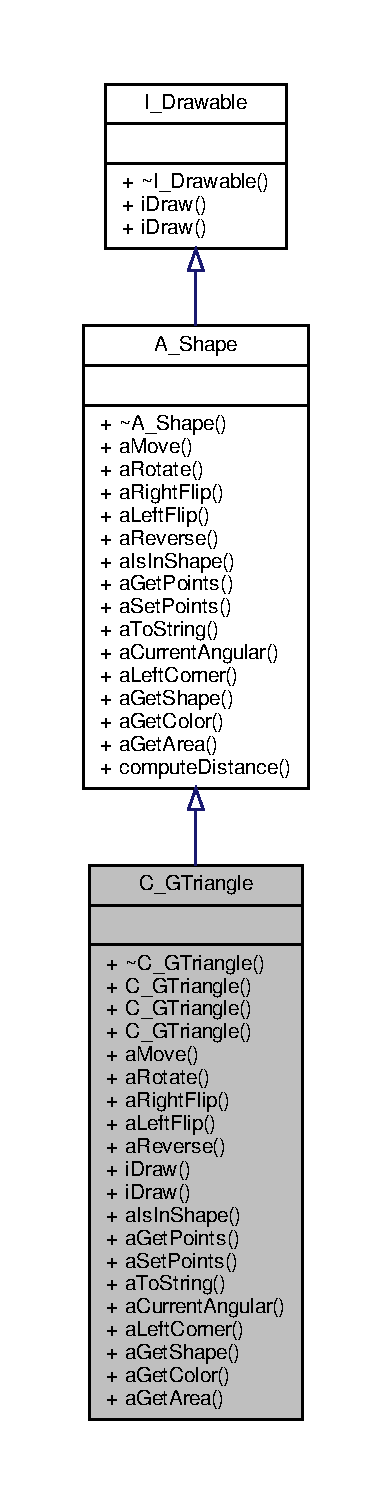
\includegraphics[height=550pt]{classC__GTriangle__inherit__graph}
\end{center}
\end{figure}


Collaboration diagram for C\+\_\+\+G\+Triangle\+:\nopagebreak
\begin{figure}[H]
\begin{center}
\leavevmode
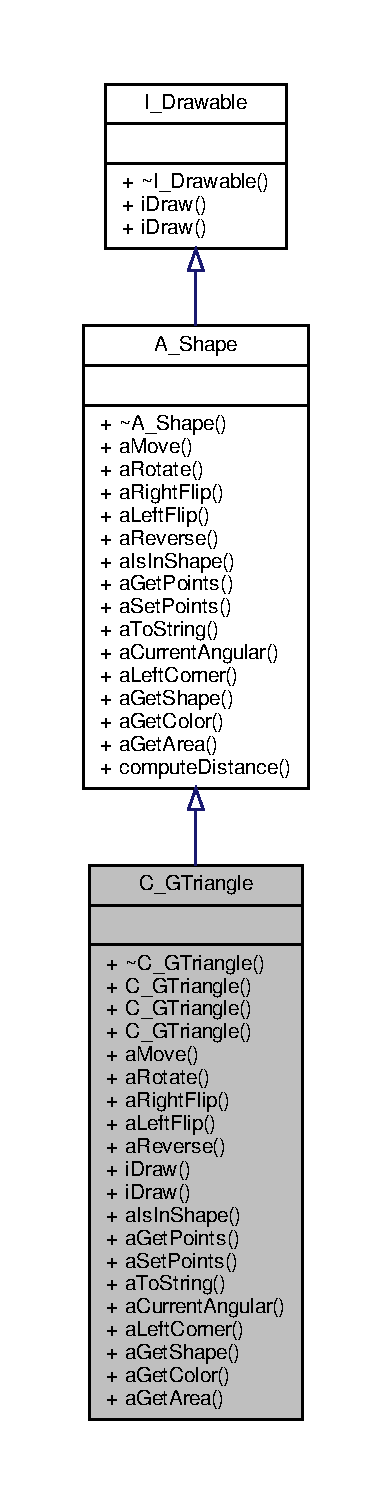
\includegraphics[height=550pt]{classC__GTriangle__coll__graph}
\end{center}
\end{figure}
\subsection*{Public Member Functions}
\begin{DoxyCompactItemize}
\item 
\hyperlink{classC__GTriangle_ad904f86d6bde64caabd005b3bad333e2}{$\sim$\+C\+\_\+\+G\+Triangle} () override
\begin{DoxyCompactList}\small\item\em Destructor of \hyperlink{classC__GTriangle}{C\+\_\+\+G\+Triangle}. \end{DoxyCompactList}\item 
\hyperlink{classC__GTriangle_aba5786a8cd754d526758e05df3f70a51}{C\+\_\+\+G\+Triangle} (M\+L\+V\+\_\+\+Color color=M\+L\+V\+\_\+\+C\+O\+L\+O\+R\+\_\+\+R\+ED)
\begin{DoxyCompactList}\small\item\em Constructor by default of \hyperlink{classC__GTriangle}{C\+\_\+\+G\+Triangle}, make a \hyperlink{classC__GTriangle}{C\+\_\+\+G\+Triangle} as default. \end{DoxyCompactList}\item 
\hyperlink{classC__GTriangle_a45212ea205ed1860ac57b048af9fd984}{C\+\_\+\+G\+Triangle} (const std\+::vector$<$ \hyperlink{classC__STriangle}{C\+\_\+\+S\+Triangle} $>$ \&triangle, M\+L\+V\+\_\+\+Color color=M\+L\+V\+\_\+\+C\+O\+L\+O\+R\+\_\+\+R\+ED)
\begin{DoxyCompactList}\small\item\em Constructor of \hyperlink{classC__GTriangle}{C\+\_\+\+G\+Triangle}, requires a vector of triangles. \end{DoxyCompactList}\item 
\hyperlink{classC__GTriangle_a2dc558251c2bd2591451e61f0d66714b}{C\+\_\+\+G\+Triangle} (const \hyperlink{classT__Point}{T\+\_\+\+Point}$<$ double $>$ \&origin, double angular=0.\+0, M\+L\+V\+\_\+\+Color color=M\+L\+V\+\_\+\+C\+O\+L\+O\+R\+\_\+\+R\+ED)
\begin{DoxyCompactList}\small\item\em Constructor of \hyperlink{classC__GTriangle}{C\+\_\+\+G\+Triangle}, calls the deleguate Default Constructor. \end{DoxyCompactList}\item 
void \hyperlink{classC__GTriangle_a07789441ce75f81fd4c4649a0115edbe}{a\+Move} (const \hyperlink{classT__Point}{T\+\_\+\+Point}$<$ double $>$ \&translation) override
\begin{DoxyCompactList}\small\item\em Move the \hyperlink{classC__GTriangle}{C\+\_\+\+G\+Triangle} by point translation. \end{DoxyCompactList}\item 
void \hyperlink{classC__GTriangle_a29c641aea4ef5fa4224b42dffc5fefa5}{a\+Rotate} (double angular) override
\begin{DoxyCompactList}\small\item\em Rotate the \hyperlink{classC__GTriangle}{C\+\_\+\+G\+Triangle} with specified angular. \end{DoxyCompactList}\item 
void \hyperlink{classC__GTriangle_aa4f808a02ae18bd36c205a5d70eb3fef}{a\+Right\+Flip} () override
\begin{DoxyCompactList}\small\item\em Flip the figure as 45° clock. \end{DoxyCompactList}\item 
void \hyperlink{classC__GTriangle_a9ffdddb586b42757ffca6a9ca0c20934}{a\+Left\+Flip} () override
\begin{DoxyCompactList}\small\item\em Flip the figure as 45° anti clock. \end{DoxyCompactList}\item 
void \hyperlink{classC__GTriangle_a479646fa1265aaf2299b59787c394a27}{a\+Reverse} () override
\begin{DoxyCompactList}\small\item\em Reverse the figure as symmetry. \end{DoxyCompactList}\item 
void \hyperlink{classC__GTriangle_a53abbd8cd622323fc2f3b80ce91cfde9}{i\+Draw} () override
\begin{DoxyCompactList}\small\item\em Draw this shape on I\+HM. \end{DoxyCompactList}\item 
void \hyperlink{classC__GTriangle_a9cfd20cb1d19e6c92bd217c470c86405}{i\+Draw} (M\+L\+V\+\_\+\+Color color) override
\begin{DoxyCompactList}\small\item\em Draw this shape on I\+HM with a specific m\+Color. \end{DoxyCompactList}\item 
bool \hyperlink{classC__GTriangle_a417b28c74dd35f81a19b5bd1d214ba8d}{a\+Is\+In\+Shape} (const \hyperlink{classT__Point}{T\+\_\+\+Point}$<$ double $>$ \&click) override
\begin{DoxyCompactList}\small\item\em Check if a point is in this shape. \end{DoxyCompactList}\item 
std\+::vector$<$ \hyperlink{classT__Point}{T\+\_\+\+Point}$<$ double $>$ $>$ \hyperlink{classC__GTriangle_af3c514a6f5516c297374004a94788877}{a\+Get\+Points} () override
\begin{DoxyCompactList}\small\item\em Get m\+Points of this shape. \end{DoxyCompactList}\item 
bool \hyperlink{classC__GTriangle_a18c134ddf90bc4f5729064a47094068b}{a\+Set\+Points} (const \hyperlink{classT__Point}{T\+\_\+\+Point}$<$ double $>$ \&ref, const \hyperlink{classT__Point}{T\+\_\+\+Point}$<$ double $>$ \&changed) override
\begin{DoxyCompactList}\small\item\em Set m\+Points of this shape. \end{DoxyCompactList}\item 
std\+::string \hyperlink{classC__GTriangle_aa432e8b8320db8a53ef1d59b486ed7ce}{a\+To\+String} () override
\begin{DoxyCompactList}\small\item\em Convert all data of \hyperlink{classC__GTriangle}{C\+\_\+\+G\+Triangle} in a string. \end{DoxyCompactList}\item 
double \hyperlink{classC__GTriangle_a98866648972bb78707c61aa7ebc22fb9}{a\+Current\+Angular} () override
\begin{DoxyCompactList}\small\item\em Get the current angular of this shape. \end{DoxyCompactList}\item 
\hyperlink{classT__Point}{T\+\_\+\+Point}$<$ double $>$ \hyperlink{classC__GTriangle_a57943afaad0f6b7c3c13aa35a233e93b}{a\+Left\+Corner} () override
\begin{DoxyCompactList}\small\item\em Take the point at left top corner. \end{DoxyCompactList}\item 
std\+::string \hyperlink{classC__GTriangle_a039e79bb17dae01997b11243de457d98}{a\+Get\+Shape} () override
\begin{DoxyCompactList}\small\item\em Get the shape type. \end{DoxyCompactList}\item 
M\+L\+V\+\_\+\+Color \hyperlink{classC__GTriangle_a19100d603f9239fd66f1115c4358f0fc}{a\+Get\+Color} () override
\begin{DoxyCompactList}\small\item\em Get the color of the shape. \end{DoxyCompactList}\item 
double \hyperlink{classC__GTriangle_a4d1c9a050aef86a7eab973b1fe668544}{a\+Get\+Area} () override
\begin{DoxyCompactList}\small\item\em Get the area of the shape. \end{DoxyCompactList}\item 
\hyperlink{classC__GTriangle_ad904f86d6bde64caabd005b3bad333e2}{$\sim$\+C\+\_\+\+G\+Triangle} () override
\begin{DoxyCompactList}\small\item\em Destructor of \hyperlink{classC__GTriangle}{C\+\_\+\+G\+Triangle}. \end{DoxyCompactList}\item 
\hyperlink{classC__GTriangle_aba5786a8cd754d526758e05df3f70a51}{C\+\_\+\+G\+Triangle} (M\+L\+V\+\_\+\+Color color=M\+L\+V\+\_\+\+C\+O\+L\+O\+R\+\_\+\+R\+ED)
\begin{DoxyCompactList}\small\item\em Constructor by default of \hyperlink{classC__GTriangle}{C\+\_\+\+G\+Triangle}, make a \hyperlink{classC__GTriangle}{C\+\_\+\+G\+Triangle} as default. \end{DoxyCompactList}\item 
\hyperlink{classC__GTriangle_a45212ea205ed1860ac57b048af9fd984}{C\+\_\+\+G\+Triangle} (const std\+::vector$<$ \hyperlink{classC__STriangle}{C\+\_\+\+S\+Triangle} $>$ \&triangle, M\+L\+V\+\_\+\+Color color=M\+L\+V\+\_\+\+C\+O\+L\+O\+R\+\_\+\+R\+ED)
\begin{DoxyCompactList}\small\item\em Constructor of \hyperlink{classC__GTriangle}{C\+\_\+\+G\+Triangle}, requires a vector of triangles. \end{DoxyCompactList}\item 
\hyperlink{classC__GTriangle_a2dc558251c2bd2591451e61f0d66714b}{C\+\_\+\+G\+Triangle} (const \hyperlink{classT__Point}{T\+\_\+\+Point}$<$ double $>$ \&origin, double angular=0.\+0, M\+L\+V\+\_\+\+Color color=M\+L\+V\+\_\+\+C\+O\+L\+O\+R\+\_\+\+R\+ED)
\begin{DoxyCompactList}\small\item\em Constructor of \hyperlink{classC__GTriangle}{C\+\_\+\+G\+Triangle}, calls the deleguate Default Constructor. \end{DoxyCompactList}\item 
void \hyperlink{classC__GTriangle_a07789441ce75f81fd4c4649a0115edbe}{a\+Move} (const \hyperlink{classT__Point}{T\+\_\+\+Point}$<$ double $>$ \&translation) override
\begin{DoxyCompactList}\small\item\em Move the \hyperlink{classC__GTriangle}{C\+\_\+\+G\+Triangle} by point translation. \end{DoxyCompactList}\item 
void \hyperlink{classC__GTriangle_a29c641aea4ef5fa4224b42dffc5fefa5}{a\+Rotate} (double angular) override
\begin{DoxyCompactList}\small\item\em Rotate the \hyperlink{classC__GTriangle}{C\+\_\+\+G\+Triangle} with specified angular. \end{DoxyCompactList}\item 
void \hyperlink{classC__GTriangle_aa4f808a02ae18bd36c205a5d70eb3fef}{a\+Right\+Flip} () override
\begin{DoxyCompactList}\small\item\em Flip the figure as 45° clock. \end{DoxyCompactList}\item 
void \hyperlink{classC__GTriangle_a9ffdddb586b42757ffca6a9ca0c20934}{a\+Left\+Flip} () override
\begin{DoxyCompactList}\small\item\em Flip the figure as 45° anti clock. \end{DoxyCompactList}\item 
void \hyperlink{classC__GTriangle_a479646fa1265aaf2299b59787c394a27}{a\+Reverse} () override
\begin{DoxyCompactList}\small\item\em Reverse the figure as symmetry. \end{DoxyCompactList}\item 
void \hyperlink{classC__GTriangle_a53abbd8cd622323fc2f3b80ce91cfde9}{i\+Draw} () override
\begin{DoxyCompactList}\small\item\em Draw this shape on I\+HM. \end{DoxyCompactList}\item 
void \hyperlink{classC__GTriangle_a9cfd20cb1d19e6c92bd217c470c86405}{i\+Draw} (M\+L\+V\+\_\+\+Color color) override
\begin{DoxyCompactList}\small\item\em Draw this shape on I\+HM with a specific m\+Color. \end{DoxyCompactList}\item 
bool \hyperlink{classC__GTriangle_a417b28c74dd35f81a19b5bd1d214ba8d}{a\+Is\+In\+Shape} (const \hyperlink{classT__Point}{T\+\_\+\+Point}$<$ double $>$ \&click) override
\begin{DoxyCompactList}\small\item\em Check if a point is in this shape. \end{DoxyCompactList}\item 
std\+::vector$<$ \hyperlink{classT__Point}{T\+\_\+\+Point}$<$ double $>$ $>$ \hyperlink{classC__GTriangle_aa18970aab947266cab2d4a9f664926a0}{a\+Get\+Points} () override
\begin{DoxyCompactList}\small\item\em Get m\+Points of this shape. \end{DoxyCompactList}\item 
bool \hyperlink{classC__GTriangle_a18c134ddf90bc4f5729064a47094068b}{a\+Set\+Points} (const \hyperlink{classT__Point}{T\+\_\+\+Point}$<$ double $>$ \&ref, const \hyperlink{classT__Point}{T\+\_\+\+Point}$<$ double $>$ \&changed) override
\begin{DoxyCompactList}\small\item\em Set m\+Points of this shape. \end{DoxyCompactList}\item 
std\+::string \hyperlink{classC__GTriangle_aa432e8b8320db8a53ef1d59b486ed7ce}{a\+To\+String} () override
\begin{DoxyCompactList}\small\item\em Convert all data of \hyperlink{classC__GTriangle}{C\+\_\+\+G\+Triangle} in a string. \end{DoxyCompactList}\item 
double \hyperlink{classC__GTriangle_a98866648972bb78707c61aa7ebc22fb9}{a\+Current\+Angular} () override
\begin{DoxyCompactList}\small\item\em Get the current angular of this shape. \end{DoxyCompactList}\item 
\hyperlink{classT__Point}{T\+\_\+\+Point}$<$ double $>$ \hyperlink{classC__GTriangle_a527bdcfbcba0747c0d16d0472d0b15d8}{a\+Left\+Corner} () override
\begin{DoxyCompactList}\small\item\em Take the point at left top corner. \end{DoxyCompactList}\item 
std\+::string \hyperlink{classC__GTriangle_a039e79bb17dae01997b11243de457d98}{a\+Get\+Shape} () override
\begin{DoxyCompactList}\small\item\em Get the shape type. \end{DoxyCompactList}\item 
M\+L\+V\+\_\+\+Color \hyperlink{classC__GTriangle_a19100d603f9239fd66f1115c4358f0fc}{a\+Get\+Color} () override
\begin{DoxyCompactList}\small\item\em Get the color of the shape. \end{DoxyCompactList}\item 
double \hyperlink{classC__GTriangle_a4d1c9a050aef86a7eab973b1fe668544}{a\+Get\+Area} () override
\begin{DoxyCompactList}\small\item\em Get the area of the shape. \end{DoxyCompactList}\end{DoxyCompactItemize}
\subsection*{Additional Inherited Members}


\subsection{Detailed Description}
Class of the greatest m\+Triangles. 

This class manage everything about the greatest m\+Triangles 

\subsection{Constructor \& Destructor Documentation}
\mbox{\Hypertarget{classC__GTriangle_ad904f86d6bde64caabd005b3bad333e2}\label{classC__GTriangle_ad904f86d6bde64caabd005b3bad333e2}} 
\index{C\+\_\+\+G\+Triangle@{C\+\_\+\+G\+Triangle}!````~C\+\_\+\+G\+Triangle@{$\sim$\+C\+\_\+\+G\+Triangle}}
\index{````~C\+\_\+\+G\+Triangle@{$\sim$\+C\+\_\+\+G\+Triangle}!C\+\_\+\+G\+Triangle@{C\+\_\+\+G\+Triangle}}
\subsubsection{\texorpdfstring{$\sim$\+C\+\_\+\+G\+Triangle()}{~C\_GTriangle()}\hspace{0.1cm}{\footnotesize\ttfamily [1/2]}}
{\footnotesize\ttfamily C\+\_\+\+G\+Triangle\+::$\sim$\+C\+\_\+\+G\+Triangle (\begin{DoxyParamCaption}{ }\end{DoxyParamCaption})\hspace{0.3cm}{\ttfamily [override]}}



Destructor of \hyperlink{classC__GTriangle}{C\+\_\+\+G\+Triangle}. 

\mbox{\Hypertarget{classC__GTriangle_aba5786a8cd754d526758e05df3f70a51}\label{classC__GTriangle_aba5786a8cd754d526758e05df3f70a51}} 
\index{C\+\_\+\+G\+Triangle@{C\+\_\+\+G\+Triangle}!C\+\_\+\+G\+Triangle@{C\+\_\+\+G\+Triangle}}
\index{C\+\_\+\+G\+Triangle@{C\+\_\+\+G\+Triangle}!C\+\_\+\+G\+Triangle@{C\+\_\+\+G\+Triangle}}
\subsubsection{\texorpdfstring{C\+\_\+\+G\+Triangle()}{C\_GTriangle()}\hspace{0.1cm}{\footnotesize\ttfamily [1/6]}}
{\footnotesize\ttfamily C\+\_\+\+G\+Triangle\+::\+C\+\_\+\+G\+Triangle (\begin{DoxyParamCaption}\item[{M\+L\+V\+\_\+\+Color}]{color = {\ttfamily MLV\+\_\+COLOR\+\_\+RED} }\end{DoxyParamCaption})\hspace{0.3cm}{\ttfamily [explicit]}}



Constructor by default of \hyperlink{classC__GTriangle}{C\+\_\+\+G\+Triangle}, make a \hyperlink{classC__GTriangle}{C\+\_\+\+G\+Triangle} as default. 


\begin{DoxyParams}{Parameters}
{\em color} & \+: Optional \+\_\+\+\_\+\+Parameter, m\+Color of this shape \\
\hline
\end{DoxyParams}
\mbox{\Hypertarget{classC__GTriangle_a45212ea205ed1860ac57b048af9fd984}\label{classC__GTriangle_a45212ea205ed1860ac57b048af9fd984}} 
\index{C\+\_\+\+G\+Triangle@{C\+\_\+\+G\+Triangle}!C\+\_\+\+G\+Triangle@{C\+\_\+\+G\+Triangle}}
\index{C\+\_\+\+G\+Triangle@{C\+\_\+\+G\+Triangle}!C\+\_\+\+G\+Triangle@{C\+\_\+\+G\+Triangle}}
\subsubsection{\texorpdfstring{C\+\_\+\+G\+Triangle()}{C\_GTriangle()}\hspace{0.1cm}{\footnotesize\ttfamily [2/6]}}
{\footnotesize\ttfamily C\+\_\+\+G\+Triangle\+::\+C\+\_\+\+G\+Triangle (\begin{DoxyParamCaption}\item[{const std\+::vector$<$ \hyperlink{classC__STriangle}{C\+\_\+\+S\+Triangle} $>$ \&}]{triangle,  }\item[{M\+L\+V\+\_\+\+Color}]{color = {\ttfamily MLV\+\_\+COLOR\+\_\+RED} }\end{DoxyParamCaption})\hspace{0.3cm}{\ttfamily [explicit]}}



Constructor of \hyperlink{classC__GTriangle}{C\+\_\+\+G\+Triangle}, requires a vector of triangles. 


\begin{DoxyParams}{Parameters}
{\em triangle} & \+: The \hyperlink{classC__GTriangle}{C\+\_\+\+G\+Triangle} will created with a vector of \hyperlink{classC__STriangle}{C\+\_\+\+S\+Triangle} (4) \\
\hline
{\em color} & \+: Optional \+\_\+\+\_\+\+Parameter, m\+Color of this shape \\
\hline
\end{DoxyParams}
\mbox{\Hypertarget{classC__GTriangle_a2dc558251c2bd2591451e61f0d66714b}\label{classC__GTriangle_a2dc558251c2bd2591451e61f0d66714b}} 
\index{C\+\_\+\+G\+Triangle@{C\+\_\+\+G\+Triangle}!C\+\_\+\+G\+Triangle@{C\+\_\+\+G\+Triangle}}
\index{C\+\_\+\+G\+Triangle@{C\+\_\+\+G\+Triangle}!C\+\_\+\+G\+Triangle@{C\+\_\+\+G\+Triangle}}
\subsubsection{\texorpdfstring{C\+\_\+\+G\+Triangle()}{C\_GTriangle()}\hspace{0.1cm}{\footnotesize\ttfamily [3/6]}}
{\footnotesize\ttfamily C\+\_\+\+G\+Triangle\+::\+C\+\_\+\+G\+Triangle (\begin{DoxyParamCaption}\item[{const \hyperlink{classT__Point}{T\+\_\+\+Point}$<$ double $>$ \&}]{origin,  }\item[{double}]{angular = {\ttfamily 0.0},  }\item[{M\+L\+V\+\_\+\+Color}]{color = {\ttfamily MLV\+\_\+COLOR\+\_\+RED} }\end{DoxyParamCaption})\hspace{0.3cm}{\ttfamily [explicit]}}



Constructor of \hyperlink{classC__GTriangle}{C\+\_\+\+G\+Triangle}, calls the deleguate Default Constructor. 


\begin{DoxyParams}{Parameters}
{\em origin} & \+: shifts the figure of a translation of the origin \\
\hline
{\em angular} & \+: Optional \+\_\+\+\_\+\+Parameter (angular=0.\+0 as default), a\+Rotate the figure with an angular \\
\hline
{\em color} & \+: Optional \+\_\+\+\_\+\+Parameter, m\+Color of this shape \\
\hline
\end{DoxyParams}
\mbox{\Hypertarget{classC__GTriangle_ad904f86d6bde64caabd005b3bad333e2}\label{classC__GTriangle_ad904f86d6bde64caabd005b3bad333e2}} 
\index{C\+\_\+\+G\+Triangle@{C\+\_\+\+G\+Triangle}!````~C\+\_\+\+G\+Triangle@{$\sim$\+C\+\_\+\+G\+Triangle}}
\index{````~C\+\_\+\+G\+Triangle@{$\sim$\+C\+\_\+\+G\+Triangle}!C\+\_\+\+G\+Triangle@{C\+\_\+\+G\+Triangle}}
\subsubsection{\texorpdfstring{$\sim$\+C\+\_\+\+G\+Triangle()}{~C\_GTriangle()}\hspace{0.1cm}{\footnotesize\ttfamily [2/2]}}
{\footnotesize\ttfamily C\+\_\+\+G\+Triangle\+::$\sim$\+C\+\_\+\+G\+Triangle (\begin{DoxyParamCaption}{ }\end{DoxyParamCaption})\hspace{0.3cm}{\ttfamily [override]}}



Destructor of \hyperlink{classC__GTriangle}{C\+\_\+\+G\+Triangle}. 

\mbox{\Hypertarget{classC__GTriangle_aba5786a8cd754d526758e05df3f70a51}\label{classC__GTriangle_aba5786a8cd754d526758e05df3f70a51}} 
\index{C\+\_\+\+G\+Triangle@{C\+\_\+\+G\+Triangle}!C\+\_\+\+G\+Triangle@{C\+\_\+\+G\+Triangle}}
\index{C\+\_\+\+G\+Triangle@{C\+\_\+\+G\+Triangle}!C\+\_\+\+G\+Triangle@{C\+\_\+\+G\+Triangle}}
\subsubsection{\texorpdfstring{C\+\_\+\+G\+Triangle()}{C\_GTriangle()}\hspace{0.1cm}{\footnotesize\ttfamily [4/6]}}
{\footnotesize\ttfamily C\+\_\+\+G\+Triangle\+::\+C\+\_\+\+G\+Triangle (\begin{DoxyParamCaption}\item[{M\+L\+V\+\_\+\+Color}]{color = {\ttfamily MLV\+\_\+COLOR\+\_\+RED} }\end{DoxyParamCaption})\hspace{0.3cm}{\ttfamily [explicit]}}



Constructor by default of \hyperlink{classC__GTriangle}{C\+\_\+\+G\+Triangle}, make a \hyperlink{classC__GTriangle}{C\+\_\+\+G\+Triangle} as default. 


\begin{DoxyParams}{Parameters}
{\em color} & \+: Optional \+\_\+\+\_\+\+Parameter, m\+Color of this shape \\
\hline
\end{DoxyParams}
\mbox{\Hypertarget{classC__GTriangle_a45212ea205ed1860ac57b048af9fd984}\label{classC__GTriangle_a45212ea205ed1860ac57b048af9fd984}} 
\index{C\+\_\+\+G\+Triangle@{C\+\_\+\+G\+Triangle}!C\+\_\+\+G\+Triangle@{C\+\_\+\+G\+Triangle}}
\index{C\+\_\+\+G\+Triangle@{C\+\_\+\+G\+Triangle}!C\+\_\+\+G\+Triangle@{C\+\_\+\+G\+Triangle}}
\subsubsection{\texorpdfstring{C\+\_\+\+G\+Triangle()}{C\_GTriangle()}\hspace{0.1cm}{\footnotesize\ttfamily [5/6]}}
{\footnotesize\ttfamily C\+\_\+\+G\+Triangle\+::\+C\+\_\+\+G\+Triangle (\begin{DoxyParamCaption}\item[{const std\+::vector$<$ \hyperlink{classC__STriangle}{C\+\_\+\+S\+Triangle} $>$ \&}]{triangle,  }\item[{M\+L\+V\+\_\+\+Color}]{color = {\ttfamily MLV\+\_\+COLOR\+\_\+RED} }\end{DoxyParamCaption})\hspace{0.3cm}{\ttfamily [explicit]}}



Constructor of \hyperlink{classC__GTriangle}{C\+\_\+\+G\+Triangle}, requires a vector of triangles. 


\begin{DoxyParams}{Parameters}
{\em triangle} & \+: The \hyperlink{classC__GTriangle}{C\+\_\+\+G\+Triangle} will created with a vector of \hyperlink{classC__STriangle}{C\+\_\+\+S\+Triangle} (4) \\
\hline
{\em color} & \+: Optional \+\_\+\+\_\+\+Parameter, m\+Color of this shape \\
\hline
\end{DoxyParams}
\mbox{\Hypertarget{classC__GTriangle_a2dc558251c2bd2591451e61f0d66714b}\label{classC__GTriangle_a2dc558251c2bd2591451e61f0d66714b}} 
\index{C\+\_\+\+G\+Triangle@{C\+\_\+\+G\+Triangle}!C\+\_\+\+G\+Triangle@{C\+\_\+\+G\+Triangle}}
\index{C\+\_\+\+G\+Triangle@{C\+\_\+\+G\+Triangle}!C\+\_\+\+G\+Triangle@{C\+\_\+\+G\+Triangle}}
\subsubsection{\texorpdfstring{C\+\_\+\+G\+Triangle()}{C\_GTriangle()}\hspace{0.1cm}{\footnotesize\ttfamily [6/6]}}
{\footnotesize\ttfamily C\+\_\+\+G\+Triangle\+::\+C\+\_\+\+G\+Triangle (\begin{DoxyParamCaption}\item[{const \hyperlink{classT__Point}{T\+\_\+\+Point}$<$ double $>$ \&}]{origin,  }\item[{double}]{angular = {\ttfamily 0.0},  }\item[{M\+L\+V\+\_\+\+Color}]{color = {\ttfamily MLV\+\_\+COLOR\+\_\+RED} }\end{DoxyParamCaption})\hspace{0.3cm}{\ttfamily [explicit]}}



Constructor of \hyperlink{classC__GTriangle}{C\+\_\+\+G\+Triangle}, calls the deleguate Default Constructor. 


\begin{DoxyParams}{Parameters}
{\em origin} & \+: shifts the figure of a translation of the origin \\
\hline
{\em angular} & \+: Optional \+\_\+\+\_\+\+Parameter (angular=0.\+0 as default), a\+Rotate the figure with an angular \\
\hline
{\em color} & \+: Optional \+\_\+\+\_\+\+Parameter, m\+Color of this shape \\
\hline
\end{DoxyParams}


\subsection{Member Function Documentation}
\mbox{\Hypertarget{classC__GTriangle_a98866648972bb78707c61aa7ebc22fb9}\label{classC__GTriangle_a98866648972bb78707c61aa7ebc22fb9}} 
\index{C\+\_\+\+G\+Triangle@{C\+\_\+\+G\+Triangle}!a\+Current\+Angular@{a\+Current\+Angular}}
\index{a\+Current\+Angular@{a\+Current\+Angular}!C\+\_\+\+G\+Triangle@{C\+\_\+\+G\+Triangle}}
\subsubsection{\texorpdfstring{a\+Current\+Angular()}{aCurrentAngular()}\hspace{0.1cm}{\footnotesize\ttfamily [1/2]}}
{\footnotesize\ttfamily double C\+\_\+\+G\+Triangle\+::a\+Current\+Angular (\begin{DoxyParamCaption}{ }\end{DoxyParamCaption})\hspace{0.3cm}{\ttfamily [override]}, {\ttfamily [virtual]}}



Get the current angular of this shape. 

\begin{DoxyReturn}{Returns}

\end{DoxyReturn}


Implements \hyperlink{classA__Shape_a80fa4e009c875dd0ba7fc5bfeeb43f98}{A\+\_\+\+Shape}.

\mbox{\Hypertarget{classC__GTriangle_a98866648972bb78707c61aa7ebc22fb9}\label{classC__GTriangle_a98866648972bb78707c61aa7ebc22fb9}} 
\index{C\+\_\+\+G\+Triangle@{C\+\_\+\+G\+Triangle}!a\+Current\+Angular@{a\+Current\+Angular}}
\index{a\+Current\+Angular@{a\+Current\+Angular}!C\+\_\+\+G\+Triangle@{C\+\_\+\+G\+Triangle}}
\subsubsection{\texorpdfstring{a\+Current\+Angular()}{aCurrentAngular()}\hspace{0.1cm}{\footnotesize\ttfamily [2/2]}}
{\footnotesize\ttfamily double C\+\_\+\+G\+Triangle\+::a\+Current\+Angular (\begin{DoxyParamCaption}{ }\end{DoxyParamCaption})\hspace{0.3cm}{\ttfamily [override]}, {\ttfamily [virtual]}}



Get the current angular of this shape. 

\begin{DoxyReturn}{Returns}

\end{DoxyReturn}


Implements \hyperlink{classA__Shape_a80fa4e009c875dd0ba7fc5bfeeb43f98}{A\+\_\+\+Shape}.

\mbox{\Hypertarget{classC__GTriangle_a4d1c9a050aef86a7eab973b1fe668544}\label{classC__GTriangle_a4d1c9a050aef86a7eab973b1fe668544}} 
\index{C\+\_\+\+G\+Triangle@{C\+\_\+\+G\+Triangle}!a\+Get\+Area@{a\+Get\+Area}}
\index{a\+Get\+Area@{a\+Get\+Area}!C\+\_\+\+G\+Triangle@{C\+\_\+\+G\+Triangle}}
\subsubsection{\texorpdfstring{a\+Get\+Area()}{aGetArea()}\hspace{0.1cm}{\footnotesize\ttfamily [1/2]}}
{\footnotesize\ttfamily double C\+\_\+\+G\+Triangle\+::a\+Get\+Area (\begin{DoxyParamCaption}{ }\end{DoxyParamCaption})\hspace{0.3cm}{\ttfamily [override]}, {\ttfamily [virtual]}}



Get the area of the shape. 

\begin{DoxyReturn}{Returns}
Return the area of the shape 
\end{DoxyReturn}


Implements \hyperlink{classA__Shape_a1b142ee2d873d6c217f65de1632e7b6e}{A\+\_\+\+Shape}.

\mbox{\Hypertarget{classC__GTriangle_a4d1c9a050aef86a7eab973b1fe668544}\label{classC__GTriangle_a4d1c9a050aef86a7eab973b1fe668544}} 
\index{C\+\_\+\+G\+Triangle@{C\+\_\+\+G\+Triangle}!a\+Get\+Area@{a\+Get\+Area}}
\index{a\+Get\+Area@{a\+Get\+Area}!C\+\_\+\+G\+Triangle@{C\+\_\+\+G\+Triangle}}
\subsubsection{\texorpdfstring{a\+Get\+Area()}{aGetArea()}\hspace{0.1cm}{\footnotesize\ttfamily [2/2]}}
{\footnotesize\ttfamily double C\+\_\+\+G\+Triangle\+::a\+Get\+Area (\begin{DoxyParamCaption}{ }\end{DoxyParamCaption})\hspace{0.3cm}{\ttfamily [override]}, {\ttfamily [virtual]}}



Get the area of the shape. 

\begin{DoxyReturn}{Returns}
Return the area of the shape 
\end{DoxyReturn}


Implements \hyperlink{classA__Shape_a1b142ee2d873d6c217f65de1632e7b6e}{A\+\_\+\+Shape}.

\mbox{\Hypertarget{classC__GTriangle_a19100d603f9239fd66f1115c4358f0fc}\label{classC__GTriangle_a19100d603f9239fd66f1115c4358f0fc}} 
\index{C\+\_\+\+G\+Triangle@{C\+\_\+\+G\+Triangle}!a\+Get\+Color@{a\+Get\+Color}}
\index{a\+Get\+Color@{a\+Get\+Color}!C\+\_\+\+G\+Triangle@{C\+\_\+\+G\+Triangle}}
\subsubsection{\texorpdfstring{a\+Get\+Color()}{aGetColor()}\hspace{0.1cm}{\footnotesize\ttfamily [1/2]}}
{\footnotesize\ttfamily M\+L\+V\+\_\+\+Color C\+\_\+\+G\+Triangle\+::a\+Get\+Color (\begin{DoxyParamCaption}{ }\end{DoxyParamCaption})\hspace{0.3cm}{\ttfamily [override]}, {\ttfamily [virtual]}}



Get the color of the shape. 

\begin{DoxyReturn}{Returns}
Return the M\+L\+V\+\_\+\+Color of the shape 
\end{DoxyReturn}


Implements \hyperlink{classA__Shape_a1e90c8132d33e4ac84d42f72606193b2}{A\+\_\+\+Shape}.

\mbox{\Hypertarget{classC__GTriangle_a19100d603f9239fd66f1115c4358f0fc}\label{classC__GTriangle_a19100d603f9239fd66f1115c4358f0fc}} 
\index{C\+\_\+\+G\+Triangle@{C\+\_\+\+G\+Triangle}!a\+Get\+Color@{a\+Get\+Color}}
\index{a\+Get\+Color@{a\+Get\+Color}!C\+\_\+\+G\+Triangle@{C\+\_\+\+G\+Triangle}}
\subsubsection{\texorpdfstring{a\+Get\+Color()}{aGetColor()}\hspace{0.1cm}{\footnotesize\ttfamily [2/2]}}
{\footnotesize\ttfamily M\+L\+V\+\_\+\+Color C\+\_\+\+G\+Triangle\+::a\+Get\+Color (\begin{DoxyParamCaption}{ }\end{DoxyParamCaption})\hspace{0.3cm}{\ttfamily [override]}, {\ttfamily [virtual]}}



Get the color of the shape. 

\begin{DoxyReturn}{Returns}
Return the M\+L\+V\+\_\+\+Color of the shape 
\end{DoxyReturn}


Implements \hyperlink{classA__Shape_a1e90c8132d33e4ac84d42f72606193b2}{A\+\_\+\+Shape}.

\mbox{\Hypertarget{classC__GTriangle_aa18970aab947266cab2d4a9f664926a0}\label{classC__GTriangle_aa18970aab947266cab2d4a9f664926a0}} 
\index{C\+\_\+\+G\+Triangle@{C\+\_\+\+G\+Triangle}!a\+Get\+Points@{a\+Get\+Points}}
\index{a\+Get\+Points@{a\+Get\+Points}!C\+\_\+\+G\+Triangle@{C\+\_\+\+G\+Triangle}}
\subsubsection{\texorpdfstring{a\+Get\+Points()}{aGetPoints()}\hspace{0.1cm}{\footnotesize\ttfamily [1/2]}}
{\footnotesize\ttfamily std\+::vector$<$\hyperlink{classT__Point}{T\+\_\+\+Point}$<$double$>$ $>$ C\+\_\+\+G\+Triangle\+::a\+Get\+Points (\begin{DoxyParamCaption}{ }\end{DoxyParamCaption})\hspace{0.3cm}{\ttfamily [override]}, {\ttfamily [virtual]}}



Get m\+Points of this shape. 

\begin{DoxyReturn}{Returns}
Return a vector of m\+Points of this shape 
\end{DoxyReturn}


Implements \hyperlink{classA__Shape_a9fd1285bd63b1fc88943c9969bf01a5c}{A\+\_\+\+Shape}.

\mbox{\Hypertarget{classC__GTriangle_af3c514a6f5516c297374004a94788877}\label{classC__GTriangle_af3c514a6f5516c297374004a94788877}} 
\index{C\+\_\+\+G\+Triangle@{C\+\_\+\+G\+Triangle}!a\+Get\+Points@{a\+Get\+Points}}
\index{a\+Get\+Points@{a\+Get\+Points}!C\+\_\+\+G\+Triangle@{C\+\_\+\+G\+Triangle}}
\subsubsection{\texorpdfstring{a\+Get\+Points()}{aGetPoints()}\hspace{0.1cm}{\footnotesize\ttfamily [2/2]}}
{\footnotesize\ttfamily std\+::vector$<$ \hyperlink{classT__Point}{T\+\_\+\+Point}$<$ double $>$ $>$ C\+\_\+\+G\+Triangle\+::a\+Get\+Points (\begin{DoxyParamCaption}{ }\end{DoxyParamCaption})\hspace{0.3cm}{\ttfamily [override]}, {\ttfamily [virtual]}}



Get m\+Points of this shape. 

\begin{DoxyReturn}{Returns}
Return a vector of m\+Points of this shape 
\end{DoxyReturn}


Implements \hyperlink{classA__Shape_a9fd1285bd63b1fc88943c9969bf01a5c}{A\+\_\+\+Shape}.

\mbox{\Hypertarget{classC__GTriangle_a039e79bb17dae01997b11243de457d98}\label{classC__GTriangle_a039e79bb17dae01997b11243de457d98}} 
\index{C\+\_\+\+G\+Triangle@{C\+\_\+\+G\+Triangle}!a\+Get\+Shape@{a\+Get\+Shape}}
\index{a\+Get\+Shape@{a\+Get\+Shape}!C\+\_\+\+G\+Triangle@{C\+\_\+\+G\+Triangle}}
\subsubsection{\texorpdfstring{a\+Get\+Shape()}{aGetShape()}\hspace{0.1cm}{\footnotesize\ttfamily [1/2]}}
{\footnotesize\ttfamily std\+::string C\+\_\+\+G\+Triangle\+::a\+Get\+Shape (\begin{DoxyParamCaption}{ }\end{DoxyParamCaption})\hspace{0.3cm}{\ttfamily [override]}, {\ttfamily [virtual]}}



Get the shape type. 

\begin{DoxyReturn}{Returns}
Return as string the shape type 
\end{DoxyReturn}


Implements \hyperlink{classA__Shape_a1b202256a4e5dcb0edab4ab93a37122c}{A\+\_\+\+Shape}.

\mbox{\Hypertarget{classC__GTriangle_a039e79bb17dae01997b11243de457d98}\label{classC__GTriangle_a039e79bb17dae01997b11243de457d98}} 
\index{C\+\_\+\+G\+Triangle@{C\+\_\+\+G\+Triangle}!a\+Get\+Shape@{a\+Get\+Shape}}
\index{a\+Get\+Shape@{a\+Get\+Shape}!C\+\_\+\+G\+Triangle@{C\+\_\+\+G\+Triangle}}
\subsubsection{\texorpdfstring{a\+Get\+Shape()}{aGetShape()}\hspace{0.1cm}{\footnotesize\ttfamily [2/2]}}
{\footnotesize\ttfamily std\+::string C\+\_\+\+G\+Triangle\+::a\+Get\+Shape (\begin{DoxyParamCaption}{ }\end{DoxyParamCaption})\hspace{0.3cm}{\ttfamily [override]}, {\ttfamily [virtual]}}



Get the shape type. 

\begin{DoxyReturn}{Returns}
Return as string the shape type 
\end{DoxyReturn}


Implements \hyperlink{classA__Shape_a1b202256a4e5dcb0edab4ab93a37122c}{A\+\_\+\+Shape}.

\mbox{\Hypertarget{classC__GTriangle_a417b28c74dd35f81a19b5bd1d214ba8d}\label{classC__GTriangle_a417b28c74dd35f81a19b5bd1d214ba8d}} 
\index{C\+\_\+\+G\+Triangle@{C\+\_\+\+G\+Triangle}!a\+Is\+In\+Shape@{a\+Is\+In\+Shape}}
\index{a\+Is\+In\+Shape@{a\+Is\+In\+Shape}!C\+\_\+\+G\+Triangle@{C\+\_\+\+G\+Triangle}}
\subsubsection{\texorpdfstring{a\+Is\+In\+Shape()}{aIsInShape()}\hspace{0.1cm}{\footnotesize\ttfamily [1/2]}}
{\footnotesize\ttfamily bool C\+\_\+\+G\+Triangle\+::a\+Is\+In\+Shape (\begin{DoxyParamCaption}\item[{const \hyperlink{classT__Point}{T\+\_\+\+Point}$<$ double $>$ \&}]{click }\end{DoxyParamCaption})\hspace{0.3cm}{\ttfamily [override]}, {\ttfamily [virtual]}}



Check if a point is in this shape. 


\begin{DoxyParams}{Parameters}
{\em click} & \+: \hyperlink{classT__Point}{T\+\_\+\+Point} to check \\
\hline
\end{DoxyParams}
\begin{DoxyReturn}{Returns}
true if Click is in this shape, false if not 
\end{DoxyReturn}


Implements \hyperlink{classA__Shape_a63f825cbc9780208d9a137f5c14917d0}{A\+\_\+\+Shape}.

\mbox{\Hypertarget{classC__GTriangle_a417b28c74dd35f81a19b5bd1d214ba8d}\label{classC__GTriangle_a417b28c74dd35f81a19b5bd1d214ba8d}} 
\index{C\+\_\+\+G\+Triangle@{C\+\_\+\+G\+Triangle}!a\+Is\+In\+Shape@{a\+Is\+In\+Shape}}
\index{a\+Is\+In\+Shape@{a\+Is\+In\+Shape}!C\+\_\+\+G\+Triangle@{C\+\_\+\+G\+Triangle}}
\subsubsection{\texorpdfstring{a\+Is\+In\+Shape()}{aIsInShape()}\hspace{0.1cm}{\footnotesize\ttfamily [2/2]}}
{\footnotesize\ttfamily bool C\+\_\+\+G\+Triangle\+::a\+Is\+In\+Shape (\begin{DoxyParamCaption}\item[{const \hyperlink{classT__Point}{T\+\_\+\+Point}$<$ double $>$ \&}]{click }\end{DoxyParamCaption})\hspace{0.3cm}{\ttfamily [override]}, {\ttfamily [virtual]}}



Check if a point is in this shape. 


\begin{DoxyParams}{Parameters}
{\em click} & \+: \hyperlink{classT__Point}{T\+\_\+\+Point} to check \\
\hline
\end{DoxyParams}
\begin{DoxyReturn}{Returns}
true if Click is in this shape, false if not 
\end{DoxyReturn}


Implements \hyperlink{classA__Shape_a63f825cbc9780208d9a137f5c14917d0}{A\+\_\+\+Shape}.

\mbox{\Hypertarget{classC__GTriangle_a57943afaad0f6b7c3c13aa35a233e93b}\label{classC__GTriangle_a57943afaad0f6b7c3c13aa35a233e93b}} 
\index{C\+\_\+\+G\+Triangle@{C\+\_\+\+G\+Triangle}!a\+Left\+Corner@{a\+Left\+Corner}}
\index{a\+Left\+Corner@{a\+Left\+Corner}!C\+\_\+\+G\+Triangle@{C\+\_\+\+G\+Triangle}}
\subsubsection{\texorpdfstring{a\+Left\+Corner()}{aLeftCorner()}\hspace{0.1cm}{\footnotesize\ttfamily [1/2]}}
{\footnotesize\ttfamily \hyperlink{classT__Point}{T\+\_\+\+Point}$<$ double $>$ C\+\_\+\+G\+Triangle\+::a\+Left\+Corner (\begin{DoxyParamCaption}{ }\end{DoxyParamCaption})\hspace{0.3cm}{\ttfamily [override]}, {\ttfamily [virtual]}}



Take the point at left top corner. 

\begin{DoxyReturn}{Returns}
Return the point at left top corner 
\end{DoxyReturn}


Implements \hyperlink{classA__Shape_abe6781b13037bf7ecea8ff9456b31533}{A\+\_\+\+Shape}.

\mbox{\Hypertarget{classC__GTriangle_a527bdcfbcba0747c0d16d0472d0b15d8}\label{classC__GTriangle_a527bdcfbcba0747c0d16d0472d0b15d8}} 
\index{C\+\_\+\+G\+Triangle@{C\+\_\+\+G\+Triangle}!a\+Left\+Corner@{a\+Left\+Corner}}
\index{a\+Left\+Corner@{a\+Left\+Corner}!C\+\_\+\+G\+Triangle@{C\+\_\+\+G\+Triangle}}
\subsubsection{\texorpdfstring{a\+Left\+Corner()}{aLeftCorner()}\hspace{0.1cm}{\footnotesize\ttfamily [2/2]}}
{\footnotesize\ttfamily \hyperlink{classT__Point}{T\+\_\+\+Point}$<$double$>$ C\+\_\+\+G\+Triangle\+::a\+Left\+Corner (\begin{DoxyParamCaption}{ }\end{DoxyParamCaption})\hspace{0.3cm}{\ttfamily [override]}, {\ttfamily [virtual]}}



Take the point at left top corner. 

\begin{DoxyReturn}{Returns}
Return the point at left top corner 
\end{DoxyReturn}


Implements \hyperlink{classA__Shape_abe6781b13037bf7ecea8ff9456b31533}{A\+\_\+\+Shape}.

\mbox{\Hypertarget{classC__GTriangle_a9ffdddb586b42757ffca6a9ca0c20934}\label{classC__GTriangle_a9ffdddb586b42757ffca6a9ca0c20934}} 
\index{C\+\_\+\+G\+Triangle@{C\+\_\+\+G\+Triangle}!a\+Left\+Flip@{a\+Left\+Flip}}
\index{a\+Left\+Flip@{a\+Left\+Flip}!C\+\_\+\+G\+Triangle@{C\+\_\+\+G\+Triangle}}
\subsubsection{\texorpdfstring{a\+Left\+Flip()}{aLeftFlip()}\hspace{0.1cm}{\footnotesize\ttfamily [1/2]}}
{\footnotesize\ttfamily void C\+\_\+\+G\+Triangle\+::a\+Left\+Flip (\begin{DoxyParamCaption}{ }\end{DoxyParamCaption})\hspace{0.3cm}{\ttfamily [override]}, {\ttfamily [virtual]}}



Flip the figure as 45° anti clock. 



Implements \hyperlink{classA__Shape_abe947e7003cb63be2b4f6c439533427d}{A\+\_\+\+Shape}.

\mbox{\Hypertarget{classC__GTriangle_a9ffdddb586b42757ffca6a9ca0c20934}\label{classC__GTriangle_a9ffdddb586b42757ffca6a9ca0c20934}} 
\index{C\+\_\+\+G\+Triangle@{C\+\_\+\+G\+Triangle}!a\+Left\+Flip@{a\+Left\+Flip}}
\index{a\+Left\+Flip@{a\+Left\+Flip}!C\+\_\+\+G\+Triangle@{C\+\_\+\+G\+Triangle}}
\subsubsection{\texorpdfstring{a\+Left\+Flip()}{aLeftFlip()}\hspace{0.1cm}{\footnotesize\ttfamily [2/2]}}
{\footnotesize\ttfamily void C\+\_\+\+G\+Triangle\+::a\+Left\+Flip (\begin{DoxyParamCaption}{ }\end{DoxyParamCaption})\hspace{0.3cm}{\ttfamily [override]}, {\ttfamily [virtual]}}



Flip the figure as 45° anti clock. 



Implements \hyperlink{classA__Shape_abe947e7003cb63be2b4f6c439533427d}{A\+\_\+\+Shape}.

\mbox{\Hypertarget{classC__GTriangle_a07789441ce75f81fd4c4649a0115edbe}\label{classC__GTriangle_a07789441ce75f81fd4c4649a0115edbe}} 
\index{C\+\_\+\+G\+Triangle@{C\+\_\+\+G\+Triangle}!a\+Move@{a\+Move}}
\index{a\+Move@{a\+Move}!C\+\_\+\+G\+Triangle@{C\+\_\+\+G\+Triangle}}
\subsubsection{\texorpdfstring{a\+Move()}{aMove()}\hspace{0.1cm}{\footnotesize\ttfamily [1/2]}}
{\footnotesize\ttfamily void C\+\_\+\+G\+Triangle\+::a\+Move (\begin{DoxyParamCaption}\item[{const \hyperlink{classT__Point}{T\+\_\+\+Point}$<$ double $>$ \&}]{translation }\end{DoxyParamCaption})\hspace{0.3cm}{\ttfamily [override]}, {\ttfamily [virtual]}}



Move the \hyperlink{classC__GTriangle}{C\+\_\+\+G\+Triangle} by point translation. 


\begin{DoxyParams}{Parameters}
{\em translation} & \+: Every m\+Points of this shape will be translate by this \+\_\+\+\_\+\+Parameter \\
\hline
\end{DoxyParams}


Implements \hyperlink{classA__Shape_ab284298db1b557ccfa7ba6de7a5fee2c}{A\+\_\+\+Shape}.

\mbox{\Hypertarget{classC__GTriangle_a07789441ce75f81fd4c4649a0115edbe}\label{classC__GTriangle_a07789441ce75f81fd4c4649a0115edbe}} 
\index{C\+\_\+\+G\+Triangle@{C\+\_\+\+G\+Triangle}!a\+Move@{a\+Move}}
\index{a\+Move@{a\+Move}!C\+\_\+\+G\+Triangle@{C\+\_\+\+G\+Triangle}}
\subsubsection{\texorpdfstring{a\+Move()}{aMove()}\hspace{0.1cm}{\footnotesize\ttfamily [2/2]}}
{\footnotesize\ttfamily void C\+\_\+\+G\+Triangle\+::a\+Move (\begin{DoxyParamCaption}\item[{const \hyperlink{classT__Point}{T\+\_\+\+Point}$<$ double $>$ \&}]{translation }\end{DoxyParamCaption})\hspace{0.3cm}{\ttfamily [override]}, {\ttfamily [virtual]}}



Move the \hyperlink{classC__GTriangle}{C\+\_\+\+G\+Triangle} by point translation. 


\begin{DoxyParams}{Parameters}
{\em translation} & \+: Every m\+Points of this shape will be translate by this \+\_\+\+\_\+\+Parameter \\
\hline
\end{DoxyParams}


Implements \hyperlink{classA__Shape_ab284298db1b557ccfa7ba6de7a5fee2c}{A\+\_\+\+Shape}.

\mbox{\Hypertarget{classC__GTriangle_a479646fa1265aaf2299b59787c394a27}\label{classC__GTriangle_a479646fa1265aaf2299b59787c394a27}} 
\index{C\+\_\+\+G\+Triangle@{C\+\_\+\+G\+Triangle}!a\+Reverse@{a\+Reverse}}
\index{a\+Reverse@{a\+Reverse}!C\+\_\+\+G\+Triangle@{C\+\_\+\+G\+Triangle}}
\subsubsection{\texorpdfstring{a\+Reverse()}{aReverse()}\hspace{0.1cm}{\footnotesize\ttfamily [1/2]}}
{\footnotesize\ttfamily void C\+\_\+\+G\+Triangle\+::a\+Reverse (\begin{DoxyParamCaption}{ }\end{DoxyParamCaption})\hspace{0.3cm}{\ttfamily [override]}, {\ttfamily [virtual]}}



Reverse the figure as symmetry. 



Implements \hyperlink{classA__Shape_afe2c7969d647f6358da13879a7534ecb}{A\+\_\+\+Shape}.

\mbox{\Hypertarget{classC__GTriangle_a479646fa1265aaf2299b59787c394a27}\label{classC__GTriangle_a479646fa1265aaf2299b59787c394a27}} 
\index{C\+\_\+\+G\+Triangle@{C\+\_\+\+G\+Triangle}!a\+Reverse@{a\+Reverse}}
\index{a\+Reverse@{a\+Reverse}!C\+\_\+\+G\+Triangle@{C\+\_\+\+G\+Triangle}}
\subsubsection{\texorpdfstring{a\+Reverse()}{aReverse()}\hspace{0.1cm}{\footnotesize\ttfamily [2/2]}}
{\footnotesize\ttfamily void C\+\_\+\+G\+Triangle\+::a\+Reverse (\begin{DoxyParamCaption}{ }\end{DoxyParamCaption})\hspace{0.3cm}{\ttfamily [override]}, {\ttfamily [virtual]}}



Reverse the figure as symmetry. 



Implements \hyperlink{classA__Shape_afe2c7969d647f6358da13879a7534ecb}{A\+\_\+\+Shape}.

\mbox{\Hypertarget{classC__GTriangle_aa4f808a02ae18bd36c205a5d70eb3fef}\label{classC__GTriangle_aa4f808a02ae18bd36c205a5d70eb3fef}} 
\index{C\+\_\+\+G\+Triangle@{C\+\_\+\+G\+Triangle}!a\+Right\+Flip@{a\+Right\+Flip}}
\index{a\+Right\+Flip@{a\+Right\+Flip}!C\+\_\+\+G\+Triangle@{C\+\_\+\+G\+Triangle}}
\subsubsection{\texorpdfstring{a\+Right\+Flip()}{aRightFlip()}\hspace{0.1cm}{\footnotesize\ttfamily [1/2]}}
{\footnotesize\ttfamily void C\+\_\+\+G\+Triangle\+::a\+Right\+Flip (\begin{DoxyParamCaption}{ }\end{DoxyParamCaption})\hspace{0.3cm}{\ttfamily [override]}, {\ttfamily [virtual]}}



Flip the figure as 45° clock. 



Implements \hyperlink{classA__Shape_a892688cbbad3297e00e87cce0dbfc76d}{A\+\_\+\+Shape}.

\mbox{\Hypertarget{classC__GTriangle_aa4f808a02ae18bd36c205a5d70eb3fef}\label{classC__GTriangle_aa4f808a02ae18bd36c205a5d70eb3fef}} 
\index{C\+\_\+\+G\+Triangle@{C\+\_\+\+G\+Triangle}!a\+Right\+Flip@{a\+Right\+Flip}}
\index{a\+Right\+Flip@{a\+Right\+Flip}!C\+\_\+\+G\+Triangle@{C\+\_\+\+G\+Triangle}}
\subsubsection{\texorpdfstring{a\+Right\+Flip()}{aRightFlip()}\hspace{0.1cm}{\footnotesize\ttfamily [2/2]}}
{\footnotesize\ttfamily void C\+\_\+\+G\+Triangle\+::a\+Right\+Flip (\begin{DoxyParamCaption}{ }\end{DoxyParamCaption})\hspace{0.3cm}{\ttfamily [override]}, {\ttfamily [virtual]}}



Flip the figure as 45° clock. 



Implements \hyperlink{classA__Shape_a892688cbbad3297e00e87cce0dbfc76d}{A\+\_\+\+Shape}.

\mbox{\Hypertarget{classC__GTriangle_a29c641aea4ef5fa4224b42dffc5fefa5}\label{classC__GTriangle_a29c641aea4ef5fa4224b42dffc5fefa5}} 
\index{C\+\_\+\+G\+Triangle@{C\+\_\+\+G\+Triangle}!a\+Rotate@{a\+Rotate}}
\index{a\+Rotate@{a\+Rotate}!C\+\_\+\+G\+Triangle@{C\+\_\+\+G\+Triangle}}
\subsubsection{\texorpdfstring{a\+Rotate()}{aRotate()}\hspace{0.1cm}{\footnotesize\ttfamily [1/2]}}
{\footnotesize\ttfamily void C\+\_\+\+G\+Triangle\+::a\+Rotate (\begin{DoxyParamCaption}\item[{double}]{angular }\end{DoxyParamCaption})\hspace{0.3cm}{\ttfamily [override]}, {\ttfamily [virtual]}}



Rotate the \hyperlink{classC__GTriangle}{C\+\_\+\+G\+Triangle} with specified angular. 


\begin{DoxyParams}{Parameters}
{\em angular} & \+: This angular should be between (0, 2\+PI) \\
\hline
\end{DoxyParams}


Implements \hyperlink{classA__Shape_a25b4e0c34cdb46da5382fe9c7467efaf}{A\+\_\+\+Shape}.

\mbox{\Hypertarget{classC__GTriangle_a29c641aea4ef5fa4224b42dffc5fefa5}\label{classC__GTriangle_a29c641aea4ef5fa4224b42dffc5fefa5}} 
\index{C\+\_\+\+G\+Triangle@{C\+\_\+\+G\+Triangle}!a\+Rotate@{a\+Rotate}}
\index{a\+Rotate@{a\+Rotate}!C\+\_\+\+G\+Triangle@{C\+\_\+\+G\+Triangle}}
\subsubsection{\texorpdfstring{a\+Rotate()}{aRotate()}\hspace{0.1cm}{\footnotesize\ttfamily [2/2]}}
{\footnotesize\ttfamily void C\+\_\+\+G\+Triangle\+::a\+Rotate (\begin{DoxyParamCaption}\item[{double}]{angular }\end{DoxyParamCaption})\hspace{0.3cm}{\ttfamily [override]}, {\ttfamily [virtual]}}



Rotate the \hyperlink{classC__GTriangle}{C\+\_\+\+G\+Triangle} with specified angular. 


\begin{DoxyParams}{Parameters}
{\em angular} & \+: This angular should be between (0, 2\+PI) \\
\hline
\end{DoxyParams}


Implements \hyperlink{classA__Shape_a25b4e0c34cdb46da5382fe9c7467efaf}{A\+\_\+\+Shape}.

\mbox{\Hypertarget{classC__GTriangle_a18c134ddf90bc4f5729064a47094068b}\label{classC__GTriangle_a18c134ddf90bc4f5729064a47094068b}} 
\index{C\+\_\+\+G\+Triangle@{C\+\_\+\+G\+Triangle}!a\+Set\+Points@{a\+Set\+Points}}
\index{a\+Set\+Points@{a\+Set\+Points}!C\+\_\+\+G\+Triangle@{C\+\_\+\+G\+Triangle}}
\subsubsection{\texorpdfstring{a\+Set\+Points()}{aSetPoints()}\hspace{0.1cm}{\footnotesize\ttfamily [1/2]}}
{\footnotesize\ttfamily bool C\+\_\+\+G\+Triangle\+::a\+Set\+Points (\begin{DoxyParamCaption}\item[{const \hyperlink{classT__Point}{T\+\_\+\+Point}$<$ double $>$ \&}]{ref,  }\item[{const \hyperlink{classT__Point}{T\+\_\+\+Point}$<$ double $>$ \&}]{changed }\end{DoxyParamCaption})\hspace{0.3cm}{\ttfamily [override]}, {\ttfamily [virtual]}}



Set m\+Points of this shape. 

\begin{DoxyReturn}{Returns}
Return a true if something has been changed, false either 
\end{DoxyReturn}


Implements \hyperlink{classA__Shape_a6996f454b337f8425ad13cba3f7a7c35}{A\+\_\+\+Shape}.

\mbox{\Hypertarget{classC__GTriangle_a18c134ddf90bc4f5729064a47094068b}\label{classC__GTriangle_a18c134ddf90bc4f5729064a47094068b}} 
\index{C\+\_\+\+G\+Triangle@{C\+\_\+\+G\+Triangle}!a\+Set\+Points@{a\+Set\+Points}}
\index{a\+Set\+Points@{a\+Set\+Points}!C\+\_\+\+G\+Triangle@{C\+\_\+\+G\+Triangle}}
\subsubsection{\texorpdfstring{a\+Set\+Points()}{aSetPoints()}\hspace{0.1cm}{\footnotesize\ttfamily [2/2]}}
{\footnotesize\ttfamily bool C\+\_\+\+G\+Triangle\+::a\+Set\+Points (\begin{DoxyParamCaption}\item[{const \hyperlink{classT__Point}{T\+\_\+\+Point}$<$ double $>$ \&}]{ref,  }\item[{const \hyperlink{classT__Point}{T\+\_\+\+Point}$<$ double $>$ \&}]{changed }\end{DoxyParamCaption})\hspace{0.3cm}{\ttfamily [override]}, {\ttfamily [virtual]}}



Set m\+Points of this shape. 

\begin{DoxyReturn}{Returns}
Return a true if something has been changed, false either 
\end{DoxyReturn}


Implements \hyperlink{classA__Shape_a6996f454b337f8425ad13cba3f7a7c35}{A\+\_\+\+Shape}.

\mbox{\Hypertarget{classC__GTriangle_aa432e8b8320db8a53ef1d59b486ed7ce}\label{classC__GTriangle_aa432e8b8320db8a53ef1d59b486ed7ce}} 
\index{C\+\_\+\+G\+Triangle@{C\+\_\+\+G\+Triangle}!a\+To\+String@{a\+To\+String}}
\index{a\+To\+String@{a\+To\+String}!C\+\_\+\+G\+Triangle@{C\+\_\+\+G\+Triangle}}
\subsubsection{\texorpdfstring{a\+To\+String()}{aToString()}\hspace{0.1cm}{\footnotesize\ttfamily [1/2]}}
{\footnotesize\ttfamily std\+::string C\+\_\+\+G\+Triangle\+::a\+To\+String (\begin{DoxyParamCaption}{ }\end{DoxyParamCaption})\hspace{0.3cm}{\ttfamily [override]}, {\ttfamily [virtual]}}



Convert all data of \hyperlink{classC__GTriangle}{C\+\_\+\+G\+Triangle} in a string. 

\begin{DoxyReturn}{Returns}
Return a string which contains every m\+Points of this shape 
\end{DoxyReturn}


Implements \hyperlink{classA__Shape_ad8804b4e74543db374af6892367b7c2e}{A\+\_\+\+Shape}.

\mbox{\Hypertarget{classC__GTriangle_aa432e8b8320db8a53ef1d59b486ed7ce}\label{classC__GTriangle_aa432e8b8320db8a53ef1d59b486ed7ce}} 
\index{C\+\_\+\+G\+Triangle@{C\+\_\+\+G\+Triangle}!a\+To\+String@{a\+To\+String}}
\index{a\+To\+String@{a\+To\+String}!C\+\_\+\+G\+Triangle@{C\+\_\+\+G\+Triangle}}
\subsubsection{\texorpdfstring{a\+To\+String()}{aToString()}\hspace{0.1cm}{\footnotesize\ttfamily [2/2]}}
{\footnotesize\ttfamily std\+::string C\+\_\+\+G\+Triangle\+::a\+To\+String (\begin{DoxyParamCaption}{ }\end{DoxyParamCaption})\hspace{0.3cm}{\ttfamily [override]}, {\ttfamily [virtual]}}



Convert all data of \hyperlink{classC__GTriangle}{C\+\_\+\+G\+Triangle} in a string. 

\begin{DoxyReturn}{Returns}
Return a string which contains every m\+Points of this shape 
\end{DoxyReturn}


Implements \hyperlink{classA__Shape_ad8804b4e74543db374af6892367b7c2e}{A\+\_\+\+Shape}.

\mbox{\Hypertarget{classC__GTriangle_a53abbd8cd622323fc2f3b80ce91cfde9}\label{classC__GTriangle_a53abbd8cd622323fc2f3b80ce91cfde9}} 
\index{C\+\_\+\+G\+Triangle@{C\+\_\+\+G\+Triangle}!i\+Draw@{i\+Draw}}
\index{i\+Draw@{i\+Draw}!C\+\_\+\+G\+Triangle@{C\+\_\+\+G\+Triangle}}
\subsubsection{\texorpdfstring{i\+Draw()}{iDraw()}\hspace{0.1cm}{\footnotesize\ttfamily [1/4]}}
{\footnotesize\ttfamily void C\+\_\+\+G\+Triangle\+::i\+Draw (\begin{DoxyParamCaption}{ }\end{DoxyParamCaption})\hspace{0.3cm}{\ttfamily [override]}, {\ttfamily [virtual]}}



Draw this shape on I\+HM. 



Implements \hyperlink{classI__Drawable_ae24c65000977a805f52ce032321cd86f}{I\+\_\+\+Drawable}.

\mbox{\Hypertarget{classC__GTriangle_a53abbd8cd622323fc2f3b80ce91cfde9}\label{classC__GTriangle_a53abbd8cd622323fc2f3b80ce91cfde9}} 
\index{C\+\_\+\+G\+Triangle@{C\+\_\+\+G\+Triangle}!i\+Draw@{i\+Draw}}
\index{i\+Draw@{i\+Draw}!C\+\_\+\+G\+Triangle@{C\+\_\+\+G\+Triangle}}
\subsubsection{\texorpdfstring{i\+Draw()}{iDraw()}\hspace{0.1cm}{\footnotesize\ttfamily [2/4]}}
{\footnotesize\ttfamily void C\+\_\+\+G\+Triangle\+::i\+Draw (\begin{DoxyParamCaption}{ }\end{DoxyParamCaption})\hspace{0.3cm}{\ttfamily [override]}, {\ttfamily [virtual]}}



Draw this shape on I\+HM. 



Implements \hyperlink{classI__Drawable_ae24c65000977a805f52ce032321cd86f}{I\+\_\+\+Drawable}.

\mbox{\Hypertarget{classC__GTriangle_a9cfd20cb1d19e6c92bd217c470c86405}\label{classC__GTriangle_a9cfd20cb1d19e6c92bd217c470c86405}} 
\index{C\+\_\+\+G\+Triangle@{C\+\_\+\+G\+Triangle}!i\+Draw@{i\+Draw}}
\index{i\+Draw@{i\+Draw}!C\+\_\+\+G\+Triangle@{C\+\_\+\+G\+Triangle}}
\subsubsection{\texorpdfstring{i\+Draw()}{iDraw()}\hspace{0.1cm}{\footnotesize\ttfamily [3/4]}}
{\footnotesize\ttfamily void C\+\_\+\+G\+Triangle\+::i\+Draw (\begin{DoxyParamCaption}\item[{M\+L\+V\+\_\+\+Color}]{color }\end{DoxyParamCaption})\hspace{0.3cm}{\ttfamily [override]}, {\ttfamily [virtual]}}



Draw this shape on I\+HM with a specific m\+Color. 


\begin{DoxyParams}{Parameters}
{\em color} & Color used to \+\_\+\+\_\+\+Draw the shape \\
\hline
\end{DoxyParams}


Implements \hyperlink{classI__Drawable_a25f6474325614c451a91f019e5fe8010}{I\+\_\+\+Drawable}.

\mbox{\Hypertarget{classC__GTriangle_a9cfd20cb1d19e6c92bd217c470c86405}\label{classC__GTriangle_a9cfd20cb1d19e6c92bd217c470c86405}} 
\index{C\+\_\+\+G\+Triangle@{C\+\_\+\+G\+Triangle}!i\+Draw@{i\+Draw}}
\index{i\+Draw@{i\+Draw}!C\+\_\+\+G\+Triangle@{C\+\_\+\+G\+Triangle}}
\subsubsection{\texorpdfstring{i\+Draw()}{iDraw()}\hspace{0.1cm}{\footnotesize\ttfamily [4/4]}}
{\footnotesize\ttfamily void C\+\_\+\+G\+Triangle\+::i\+Draw (\begin{DoxyParamCaption}\item[{M\+L\+V\+\_\+\+Color}]{color }\end{DoxyParamCaption})\hspace{0.3cm}{\ttfamily [override]}, {\ttfamily [virtual]}}



Draw this shape on I\+HM with a specific m\+Color. 


\begin{DoxyParams}{Parameters}
{\em color} & Color used to \+\_\+\+\_\+\+Draw the shape \\
\hline
\end{DoxyParams}


Implements \hyperlink{classI__Drawable_a25f6474325614c451a91f019e5fe8010}{I\+\_\+\+Drawable}.



The documentation for this class was generated from the following files\+:\begin{DoxyCompactItemize}
\item 
include/\hyperlink{C__GTriangle_8hpp}{C\+\_\+\+G\+Triangle.\+hpp}\item 
src/shape/\hyperlink{C__GTriangle_8cpp}{C\+\_\+\+G\+Triangle.\+cpp}\end{DoxyCompactItemize}

\hypertarget{classC__Loader}{}\section{C\+\_\+\+Loader Class Reference}
\label{classC__Loader}\index{C\+\_\+\+Loader@{C\+\_\+\+Loader}}


Class of the main \hyperlink{classC__Loader}{C\+\_\+\+Loader}.  




{\ttfamily \#include $<$C\+\_\+\+Loader.\+hpp$>$}



Collaboration diagram for C\+\_\+\+Loader\+:\nopagebreak
\begin{figure}[H]
\begin{center}
\leavevmode
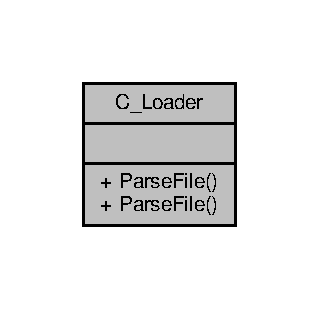
\includegraphics[width=153pt]{classC__Loader__coll__graph}
\end{center}
\end{figure}
\subsection*{Static Public Member Functions}
\begin{DoxyCompactItemize}
\item 
static bool \hyperlink{classC__Loader_a7a6f0089933a6108eb92390afe0ead80}{Parse\+File} (const std\+::string \&filename, \hyperlink{classC__Game}{C\+\_\+\+Game} \&game)
\begin{DoxyCompactList}\small\item\em Parse a file to make a board. \end{DoxyCompactList}\end{DoxyCompactItemize}


\subsection{Detailed Description}
Class of the main \hyperlink{classC__Loader}{C\+\_\+\+Loader}. 

This class manage everything about the loader 

\subsection{Member Function Documentation}
\mbox{\Hypertarget{classC__Loader_a7a6f0089933a6108eb92390afe0ead80}\label{classC__Loader_a7a6f0089933a6108eb92390afe0ead80}} 
\index{C\+\_\+\+Loader@{C\+\_\+\+Loader}!Parse\+File@{Parse\+File}}
\index{Parse\+File@{Parse\+File}!C\+\_\+\+Loader@{C\+\_\+\+Loader}}
\subsubsection{\texorpdfstring{Parse\+File()}{ParseFile()}}
{\footnotesize\ttfamily bool C\+\_\+\+Loader\+::\+Parse\+File (\begin{DoxyParamCaption}\item[{const std\+::string \&}]{filename,  }\item[{\hyperlink{classC__Game}{C\+\_\+\+Game} \&}]{game }\end{DoxyParamCaption})\hspace{0.3cm}{\ttfamily [static]}}



Parse a file to make a board. 


\begin{DoxyParams}{Parameters}
{\em filename} & \+: name of the file, this file should be located in this directory ./\+Tangram/extern/board/ \\
\hline
{\em game} & \+: The current game / board \\
\hline
\end{DoxyParams}
\begin{DoxyReturn}{Returns}
True if the game has been created, false if not 
\end{DoxyReturn}


The documentation for this class was generated from the following files\+:\begin{DoxyCompactItemize}
\item 
include/parser/\hyperlink{C__Loader_8hpp}{C\+\_\+\+Loader.\+hpp}\item 
src/parser/\hyperlink{C__Loader_8cpp}{C\+\_\+\+Loader.\+cpp}\end{DoxyCompactItemize}

\hypertarget{classC__Menu}{}\section{C\+\_\+\+Menu Class Reference}
\label{classC__Menu}\index{C\+\_\+\+Menu@{C\+\_\+\+Menu}}


\hyperlink{classC__Menu}{C\+\_\+\+Menu} of the game.  




{\ttfamily \#include $<$C\+\_\+\+Menu.\+hpp$>$}



Collaboration diagram for C\+\_\+\+Menu\+:
\nopagebreak
\begin{figure}[H]
\begin{center}
\leavevmode
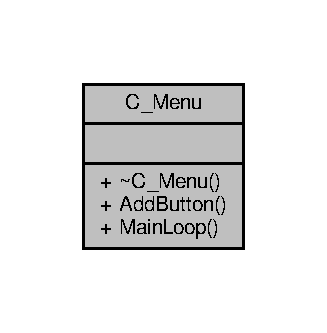
\includegraphics[width=157pt]{classC__Menu__coll__graph}
\end{center}
\end{figure}
\subsection*{Public Member Functions}
\begin{DoxyCompactItemize}
\item 
void \hyperlink{classC__Menu_a9a4f7a0022f39f35b7af9c5d2b6f31ec}{Add\+Button} (const \hyperlink{classC__Button}{C\+\_\+\+Button} \&button)
\begin{DoxyCompactList}\small\item\em Add a button in the \hyperlink{classC__Menu}{C\+\_\+\+Menu}. \end{DoxyCompactList}\item 
void \hyperlink{classC__Menu_a9529be708fad2c6deca21034bc37f59d}{Main\+Loop} ()
\begin{DoxyCompactList}\small\item\em Main loop of the \hyperlink{classC__Menu}{C\+\_\+\+Menu}. \end{DoxyCompactList}\end{DoxyCompactItemize}


\subsection{Detailed Description}
\hyperlink{classC__Menu}{C\+\_\+\+Menu} of the game. 

This class manage everything about Tangram\textquotesingle{}s menu 

\subsection{Member Function Documentation}
\mbox{\Hypertarget{classC__Menu_a9a4f7a0022f39f35b7af9c5d2b6f31ec}\label{classC__Menu_a9a4f7a0022f39f35b7af9c5d2b6f31ec}} 
\index{C\+\_\+\+Menu@{C\+\_\+\+Menu}!Add\+Button@{Add\+Button}}
\index{Add\+Button@{Add\+Button}!C\+\_\+\+Menu@{C\+\_\+\+Menu}}
\subsubsection{\texorpdfstring{Add\+Button()}{AddButton()}}
{\footnotesize\ttfamily void C\+\_\+\+Menu\+::\+Add\+Button (\begin{DoxyParamCaption}\item[{const \hyperlink{classC__Button}{C\+\_\+\+Button} \&}]{button }\end{DoxyParamCaption})}



Add a button in the \hyperlink{classC__Menu}{C\+\_\+\+Menu}. 


\begin{DoxyParams}{Parameters}
{\em button} & \+: \hyperlink{classC__Button}{C\+\_\+\+Button} to add \\
\hline
\end{DoxyParams}
\mbox{\Hypertarget{classC__Menu_a9529be708fad2c6deca21034bc37f59d}\label{classC__Menu_a9529be708fad2c6deca21034bc37f59d}} 
\index{C\+\_\+\+Menu@{C\+\_\+\+Menu}!Main\+Loop@{Main\+Loop}}
\index{Main\+Loop@{Main\+Loop}!C\+\_\+\+Menu@{C\+\_\+\+Menu}}
\subsubsection{\texorpdfstring{Main\+Loop()}{MainLoop()}}
{\footnotesize\ttfamily void C\+\_\+\+Menu\+::\+Main\+Loop (\begin{DoxyParamCaption}{ }\end{DoxyParamCaption})}



Main loop of the \hyperlink{classC__Menu}{C\+\_\+\+Menu}. 



The documentation for this class was generated from the following files\+:\begin{DoxyCompactItemize}
\item 
include/drawable/\hyperlink{C__Menu_8hpp}{C\+\_\+\+Menu.\+hpp}\item 
src/drawable/\hyperlink{C__Menu_8cpp}{C\+\_\+\+Menu.\+cpp}\end{DoxyCompactItemize}

\hypertarget{classC__MTriangle}{}\section{C\+\_\+\+M\+Triangle Class Reference}
\label{classC__MTriangle}\index{C\+\_\+\+M\+Triangle@{C\+\_\+\+M\+Triangle}}


Class of the medium \hyperlink{classC__MTriangle}{C\+\_\+\+M\+Triangle}.  




{\ttfamily \#include $<$C\+\_\+\+M\+Triangle.\+hpp$>$}



Inheritance diagram for C\+\_\+\+M\+Triangle\+:
\nopagebreak
\begin{figure}[H]
\begin{center}
\leavevmode
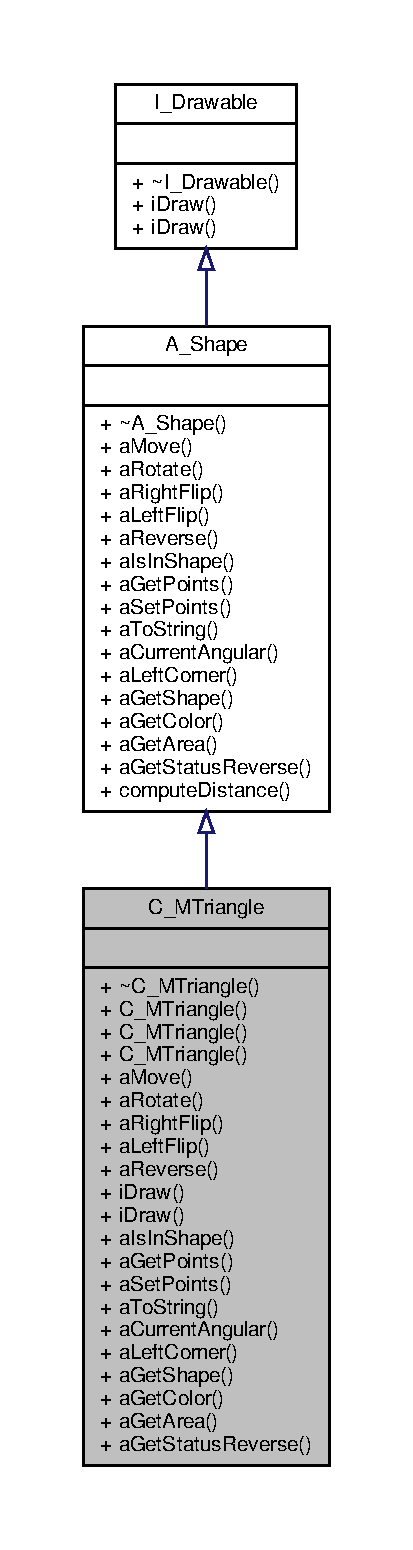
\includegraphics[height=550pt]{classC__MTriangle__inherit__graph}
\end{center}
\end{figure}


Collaboration diagram for C\+\_\+\+M\+Triangle\+:
\nopagebreak
\begin{figure}[H]
\begin{center}
\leavevmode
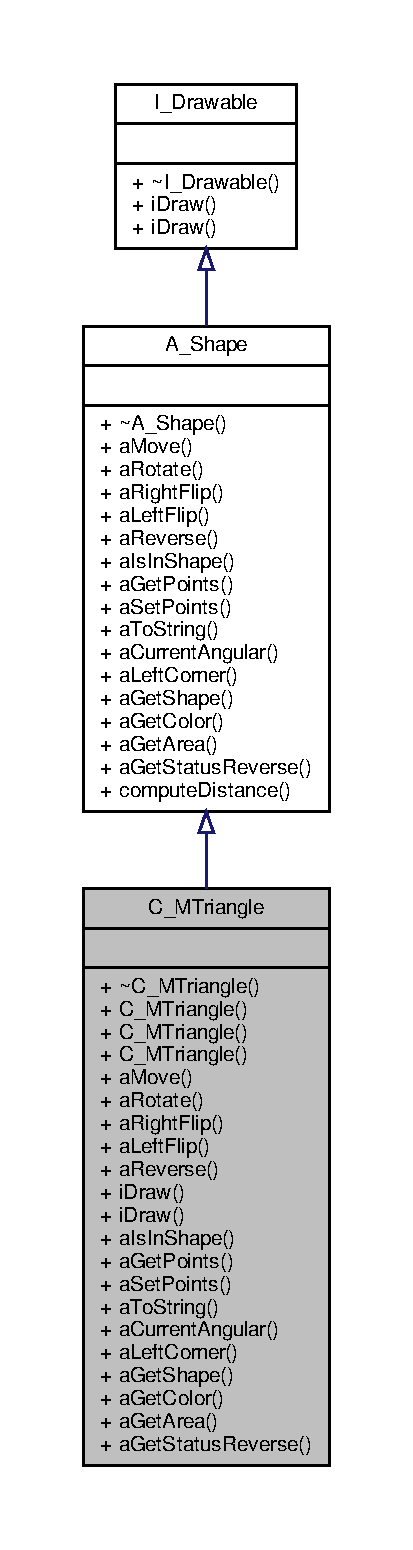
\includegraphics[height=550pt]{classC__MTriangle__coll__graph}
\end{center}
\end{figure}
\subsection*{Public Member Functions}
\begin{DoxyCompactItemize}
\item 
\hyperlink{classC__MTriangle_afec9368409c7a8bfd03cd0e735e1eee7}{$\sim$\+C\+\_\+\+M\+Triangle} () override
\begin{DoxyCompactList}\small\item\em Destructor of \hyperlink{classC__MTriangle}{C\+\_\+\+M\+Triangle}. \end{DoxyCompactList}\item 
\hyperlink{classC__MTriangle_ae9ead057d38f3e16948825353c5e31d6}{C\+\_\+\+M\+Triangle} (M\+L\+V\+\_\+\+Color color=M\+L\+V\+\_\+\+C\+O\+L\+O\+R\+\_\+\+O\+R\+A\+N\+GE)
\begin{DoxyCompactList}\small\item\em Constructor by default of \hyperlink{classC__MTriangle}{C\+\_\+\+M\+Triangle}, make a \hyperlink{classC__MTriangle}{C\+\_\+\+M\+Triangle} as default. \end{DoxyCompactList}\item 
\hyperlink{classC__MTriangle_a1a628c318d5b8982d5efa904e105ce10}{C\+\_\+\+M\+Triangle} (const std\+::vector$<$ \hyperlink{classC__STriangle}{C\+\_\+\+S\+Triangle} $>$ \&triangle, M\+L\+V\+\_\+\+Color color=M\+L\+V\+\_\+\+C\+O\+L\+O\+R\+\_\+\+O\+R\+A\+N\+GE)
\begin{DoxyCompactList}\small\item\em Constructor of \hyperlink{classC__MTriangle}{C\+\_\+\+M\+Triangle}, requires a vector of S\+Triangles. \end{DoxyCompactList}\item 
\hyperlink{classC__MTriangle_a5a8ffada7ee743f463304b1093394404}{C\+\_\+\+M\+Triangle} (const \hyperlink{classT__Point}{T\+\_\+\+Point}$<$ double $>$ \&origin, double angular=0.\+0, M\+L\+V\+\_\+\+Color color=M\+L\+V\+\_\+\+C\+O\+L\+O\+R\+\_\+\+O\+R\+A\+N\+GE)
\begin{DoxyCompactList}\small\item\em Constructor of \hyperlink{classC__MTriangle}{C\+\_\+\+M\+Triangle}, calls the deleguate Default Constructor. \end{DoxyCompactList}\item 
void \hyperlink{classC__MTriangle_a4e185345e7e1ffd5c0b7f1f8dfdbdc59}{a\+Move} (const \hyperlink{classT__Point}{T\+\_\+\+Point}$<$ double $>$ \&translation) override
\begin{DoxyCompactList}\small\item\em Move the \hyperlink{classC__MTriangle}{C\+\_\+\+M\+Triangle} by point translation. \end{DoxyCompactList}\item 
void \hyperlink{classC__MTriangle_a33aa36879be70b0a11863801da56e92e}{a\+Rotate} (double angular) override
\begin{DoxyCompactList}\small\item\em Rotate the \hyperlink{classC__MTriangle}{C\+\_\+\+M\+Triangle} with specified angular. \end{DoxyCompactList}\item 
void \hyperlink{classC__MTriangle_aa3a1fc0604fa7e13b6c89d242357a163}{a\+Right\+Flip} () override
\begin{DoxyCompactList}\small\item\em Flip the figure as 45° clock. \end{DoxyCompactList}\item 
void \hyperlink{classC__MTriangle_a3dcac8e1341a79139577deb851a6481e}{a\+Left\+Flip} () override
\begin{DoxyCompactList}\small\item\em Flip the figure as 45° anti clock. \end{DoxyCompactList}\item 
void \hyperlink{classC__MTriangle_a44614f4abb94f1a5f963cfb3e8fce7a5}{a\+Reverse} () override
\begin{DoxyCompactList}\small\item\em Reverse the figure as symmetry. \end{DoxyCompactList}\item 
void \hyperlink{classC__MTriangle_ae75dd212f0b580664affc740945c8d0b}{i\+Draw} () override
\begin{DoxyCompactList}\small\item\em Draw this shape on I\+HM. \end{DoxyCompactList}\item 
void \hyperlink{classC__MTriangle_a049e6026145865387db4244678336784}{i\+Draw} (M\+L\+V\+\_\+\+Color color) override
\begin{DoxyCompactList}\small\item\em Draw this shape on I\+HM with specific color. \end{DoxyCompactList}\item 
bool \hyperlink{classC__MTriangle_ae29e4f6608a0079507c6397b3dbef246}{a\+Is\+In\+Shape} (const \hyperlink{classT__Point}{T\+\_\+\+Point}$<$ double $>$ \&click) override
\begin{DoxyCompactList}\small\item\em Check if a point is in this shape. \end{DoxyCompactList}\item 
std\+::vector$<$ \hyperlink{classT__Point}{T\+\_\+\+Point}$<$ double $>$ $>$ \hyperlink{classC__MTriangle_ada409f8f1015cf7bf9f9ab8fb11da94b}{a\+Get\+Points} () override
\begin{DoxyCompactList}\small\item\em Get m\+Points of this shape. \end{DoxyCompactList}\item 
bool \hyperlink{classC__MTriangle_a5a3971eb0aafc16e5a34bd94130d7c6b}{a\+Set\+Points} (const \hyperlink{classT__Point}{T\+\_\+\+Point}$<$ double $>$ \&ref, const \hyperlink{classT__Point}{T\+\_\+\+Point}$<$ double $>$ \&changed) override
\begin{DoxyCompactList}\small\item\em Set a point to another one. \end{DoxyCompactList}\item 
std\+::string \hyperlink{classC__MTriangle_a3a769eb21278ec456292d88385b332a2}{a\+To\+String} () override
\begin{DoxyCompactList}\small\item\em Convert all data of \hyperlink{classC__MTriangle}{C\+\_\+\+M\+Triangle} in a string. \end{DoxyCompactList}\item 
double \hyperlink{classC__MTriangle_aad1e42f1ec9c486736a403128ba47179}{a\+Current\+Angular} () override
\begin{DoxyCompactList}\small\item\em Get the current angular of this shape. \end{DoxyCompactList}\item 
\hyperlink{classT__Point}{T\+\_\+\+Point}$<$ double $>$ \hyperlink{classC__MTriangle_ad077fce026711bf0a25fc4c1cb83ecb9}{a\+Left\+Corner} () override
\begin{DoxyCompactList}\small\item\em Take the point at left top corner. \end{DoxyCompactList}\item 
std\+::string \hyperlink{classC__MTriangle_aca7e38c6bf9695aacf54aa03ecfba978}{a\+Get\+Shape} () override
\begin{DoxyCompactList}\small\item\em Get the shape type. \end{DoxyCompactList}\item 
M\+L\+V\+\_\+\+Color \hyperlink{classC__MTriangle_aa567d77ce0e6d664beb6eea9268b1bc3}{a\+Get\+Color} () override
\begin{DoxyCompactList}\small\item\em Get the color of the shape. \end{DoxyCompactList}\item 
double \hyperlink{classC__MTriangle_a1baff5085fc1b9822987e3fc307550ce}{a\+Get\+Area} () override
\begin{DoxyCompactList}\small\item\em Get the area of the shape. \end{DoxyCompactList}\item 
bool \hyperlink{classC__MTriangle_a5c0488c23e9e64750bb879d0394830b2}{a\+Get\+Status\+Reverse} () const override
\begin{DoxyCompactList}\small\item\em Get the status of shape reversed or not. \end{DoxyCompactList}\end{DoxyCompactItemize}
\subsection*{Additional Inherited Members}


\subsection{Detailed Description}
Class of the medium \hyperlink{classC__MTriangle}{C\+\_\+\+M\+Triangle}. 

This class manage everything about the medium \hyperlink{classC__MTriangle}{C\+\_\+\+M\+Triangle} 

\subsection{Constructor \& Destructor Documentation}
\mbox{\Hypertarget{classC__MTriangle_afec9368409c7a8bfd03cd0e735e1eee7}\label{classC__MTriangle_afec9368409c7a8bfd03cd0e735e1eee7}} 
\index{C\+\_\+\+M\+Triangle@{C\+\_\+\+M\+Triangle}!````~C\+\_\+\+M\+Triangle@{$\sim$\+C\+\_\+\+M\+Triangle}}
\index{````~C\+\_\+\+M\+Triangle@{$\sim$\+C\+\_\+\+M\+Triangle}!C\+\_\+\+M\+Triangle@{C\+\_\+\+M\+Triangle}}
\subsubsection{\texorpdfstring{$\sim$\+C\+\_\+\+M\+Triangle()}{~C\_MTriangle()}}
{\footnotesize\ttfamily C\+\_\+\+M\+Triangle\+::$\sim$\+C\+\_\+\+M\+Triangle (\begin{DoxyParamCaption}{ }\end{DoxyParamCaption})\hspace{0.3cm}{\ttfamily [override]}}



Destructor of \hyperlink{classC__MTriangle}{C\+\_\+\+M\+Triangle}. 

\mbox{\Hypertarget{classC__MTriangle_ae9ead057d38f3e16948825353c5e31d6}\label{classC__MTriangle_ae9ead057d38f3e16948825353c5e31d6}} 
\index{C\+\_\+\+M\+Triangle@{C\+\_\+\+M\+Triangle}!C\+\_\+\+M\+Triangle@{C\+\_\+\+M\+Triangle}}
\index{C\+\_\+\+M\+Triangle@{C\+\_\+\+M\+Triangle}!C\+\_\+\+M\+Triangle@{C\+\_\+\+M\+Triangle}}
\subsubsection{\texorpdfstring{C\+\_\+\+M\+Triangle()}{C\_MTriangle()}\hspace{0.1cm}{\footnotesize\ttfamily [1/3]}}
{\footnotesize\ttfamily C\+\_\+\+M\+Triangle\+::\+C\+\_\+\+M\+Triangle (\begin{DoxyParamCaption}\item[{M\+L\+V\+\_\+\+Color}]{color = {\ttfamily MLV\+\_\+COLOR\+\_\+ORANGE} }\end{DoxyParamCaption})\hspace{0.3cm}{\ttfamily [explicit]}}



Constructor by default of \hyperlink{classC__MTriangle}{C\+\_\+\+M\+Triangle}, make a \hyperlink{classC__MTriangle}{C\+\_\+\+M\+Triangle} as default. 


\begin{DoxyParams}{Parameters}
{\em color} & \+: Optional \+\_\+\+\_\+\+Parameter, m\+Color of this shape \\
\hline
\end{DoxyParams}
\mbox{\Hypertarget{classC__MTriangle_a1a628c318d5b8982d5efa904e105ce10}\label{classC__MTriangle_a1a628c318d5b8982d5efa904e105ce10}} 
\index{C\+\_\+\+M\+Triangle@{C\+\_\+\+M\+Triangle}!C\+\_\+\+M\+Triangle@{C\+\_\+\+M\+Triangle}}
\index{C\+\_\+\+M\+Triangle@{C\+\_\+\+M\+Triangle}!C\+\_\+\+M\+Triangle@{C\+\_\+\+M\+Triangle}}
\subsubsection{\texorpdfstring{C\+\_\+\+M\+Triangle()}{C\_MTriangle()}\hspace{0.1cm}{\footnotesize\ttfamily [2/3]}}
{\footnotesize\ttfamily C\+\_\+\+M\+Triangle\+::\+C\+\_\+\+M\+Triangle (\begin{DoxyParamCaption}\item[{const std\+::vector$<$ \hyperlink{classC__STriangle}{C\+\_\+\+S\+Triangle} $>$ \&}]{triangle,  }\item[{M\+L\+V\+\_\+\+Color}]{color = {\ttfamily MLV\+\_\+COLOR\+\_\+ORANGE} }\end{DoxyParamCaption})\hspace{0.3cm}{\ttfamily [explicit]}}



Constructor of \hyperlink{classC__MTriangle}{C\+\_\+\+M\+Triangle}, requires a vector of S\+Triangles. 


\begin{DoxyParams}{Parameters}
{\em triangle} & \+: The \hyperlink{classC__MTriangle}{C\+\_\+\+M\+Triangle} will created with a vector of \hyperlink{classC__STriangle}{C\+\_\+\+S\+Triangle} (4) \\
\hline
{\em color} & \+: Optional \+\_\+\+\_\+\+Parameter, m\+Color of this shape \\
\hline
\end{DoxyParams}
\mbox{\Hypertarget{classC__MTriangle_a5a8ffada7ee743f463304b1093394404}\label{classC__MTriangle_a5a8ffada7ee743f463304b1093394404}} 
\index{C\+\_\+\+M\+Triangle@{C\+\_\+\+M\+Triangle}!C\+\_\+\+M\+Triangle@{C\+\_\+\+M\+Triangle}}
\index{C\+\_\+\+M\+Triangle@{C\+\_\+\+M\+Triangle}!C\+\_\+\+M\+Triangle@{C\+\_\+\+M\+Triangle}}
\subsubsection{\texorpdfstring{C\+\_\+\+M\+Triangle()}{C\_MTriangle()}\hspace{0.1cm}{\footnotesize\ttfamily [3/3]}}
{\footnotesize\ttfamily C\+\_\+\+M\+Triangle\+::\+C\+\_\+\+M\+Triangle (\begin{DoxyParamCaption}\item[{const \hyperlink{classT__Point}{T\+\_\+\+Point}$<$ double $>$ \&}]{origin,  }\item[{double}]{angular = {\ttfamily 0.0},  }\item[{M\+L\+V\+\_\+\+Color}]{color = {\ttfamily MLV\+\_\+COLOR\+\_\+ORANGE} }\end{DoxyParamCaption})\hspace{0.3cm}{\ttfamily [explicit]}}



Constructor of \hyperlink{classC__MTriangle}{C\+\_\+\+M\+Triangle}, calls the deleguate Default Constructor. 


\begin{DoxyParams}{Parameters}
{\em origin} & \+: shifts the figure of a translation of the origin \\
\hline
{\em angular} & \+: Optional \+\_\+\+\_\+\+Parameter (angular=0.\+0 as default), a\+Rotate the figure with an angular \\
\hline
{\em color} & \+: Optional \+\_\+\+\_\+\+Parameter, m\+Color of this shape \\
\hline
\end{DoxyParams}


\subsection{Member Function Documentation}
\mbox{\Hypertarget{classC__MTriangle_aad1e42f1ec9c486736a403128ba47179}\label{classC__MTriangle_aad1e42f1ec9c486736a403128ba47179}} 
\index{C\+\_\+\+M\+Triangle@{C\+\_\+\+M\+Triangle}!a\+Current\+Angular@{a\+Current\+Angular}}
\index{a\+Current\+Angular@{a\+Current\+Angular}!C\+\_\+\+M\+Triangle@{C\+\_\+\+M\+Triangle}}
\subsubsection{\texorpdfstring{a\+Current\+Angular()}{aCurrentAngular()}}
{\footnotesize\ttfamily double C\+\_\+\+M\+Triangle\+::a\+Current\+Angular (\begin{DoxyParamCaption}{ }\end{DoxyParamCaption})\hspace{0.3cm}{\ttfamily [override]}, {\ttfamily [virtual]}}



Get the current angular of this shape. 

\begin{DoxyReturn}{Returns}

\end{DoxyReturn}


Implements \hyperlink{classA__Shape_a80fa4e009c875dd0ba7fc5bfeeb43f98}{A\+\_\+\+Shape}.

\mbox{\Hypertarget{classC__MTriangle_a1baff5085fc1b9822987e3fc307550ce}\label{classC__MTriangle_a1baff5085fc1b9822987e3fc307550ce}} 
\index{C\+\_\+\+M\+Triangle@{C\+\_\+\+M\+Triangle}!a\+Get\+Area@{a\+Get\+Area}}
\index{a\+Get\+Area@{a\+Get\+Area}!C\+\_\+\+M\+Triangle@{C\+\_\+\+M\+Triangle}}
\subsubsection{\texorpdfstring{a\+Get\+Area()}{aGetArea()}}
{\footnotesize\ttfamily double C\+\_\+\+M\+Triangle\+::a\+Get\+Area (\begin{DoxyParamCaption}{ }\end{DoxyParamCaption})\hspace{0.3cm}{\ttfamily [override]}, {\ttfamily [virtual]}}



Get the area of the shape. 

\begin{DoxyReturn}{Returns}
Return the area of the shape 
\end{DoxyReturn}


Implements \hyperlink{classA__Shape_a1b142ee2d873d6c217f65de1632e7b6e}{A\+\_\+\+Shape}.

\mbox{\Hypertarget{classC__MTriangle_aa567d77ce0e6d664beb6eea9268b1bc3}\label{classC__MTriangle_aa567d77ce0e6d664beb6eea9268b1bc3}} 
\index{C\+\_\+\+M\+Triangle@{C\+\_\+\+M\+Triangle}!a\+Get\+Color@{a\+Get\+Color}}
\index{a\+Get\+Color@{a\+Get\+Color}!C\+\_\+\+M\+Triangle@{C\+\_\+\+M\+Triangle}}
\subsubsection{\texorpdfstring{a\+Get\+Color()}{aGetColor()}}
{\footnotesize\ttfamily M\+L\+V\+\_\+\+Color C\+\_\+\+M\+Triangle\+::a\+Get\+Color (\begin{DoxyParamCaption}{ }\end{DoxyParamCaption})\hspace{0.3cm}{\ttfamily [override]}, {\ttfamily [virtual]}}



Get the color of the shape. 

\begin{DoxyReturn}{Returns}
Return the M\+L\+V\+\_\+\+Color of the shape 
\end{DoxyReturn}


Implements \hyperlink{classA__Shape_a1e90c8132d33e4ac84d42f72606193b2}{A\+\_\+\+Shape}.

\mbox{\Hypertarget{classC__MTriangle_ada409f8f1015cf7bf9f9ab8fb11da94b}\label{classC__MTriangle_ada409f8f1015cf7bf9f9ab8fb11da94b}} 
\index{C\+\_\+\+M\+Triangle@{C\+\_\+\+M\+Triangle}!a\+Get\+Points@{a\+Get\+Points}}
\index{a\+Get\+Points@{a\+Get\+Points}!C\+\_\+\+M\+Triangle@{C\+\_\+\+M\+Triangle}}
\subsubsection{\texorpdfstring{a\+Get\+Points()}{aGetPoints()}}
{\footnotesize\ttfamily std\+::vector$<$ \hyperlink{classT__Point}{T\+\_\+\+Point}$<$ double $>$ $>$ C\+\_\+\+M\+Triangle\+::a\+Get\+Points (\begin{DoxyParamCaption}{ }\end{DoxyParamCaption})\hspace{0.3cm}{\ttfamily [override]}, {\ttfamily [virtual]}}



Get m\+Points of this shape. 

\begin{DoxyReturn}{Returns}
Return a vector of m\+Points of this shape 
\end{DoxyReturn}


Implements \hyperlink{classA__Shape_a9fd1285bd63b1fc88943c9969bf01a5c}{A\+\_\+\+Shape}.

\mbox{\Hypertarget{classC__MTriangle_aca7e38c6bf9695aacf54aa03ecfba978}\label{classC__MTriangle_aca7e38c6bf9695aacf54aa03ecfba978}} 
\index{C\+\_\+\+M\+Triangle@{C\+\_\+\+M\+Triangle}!a\+Get\+Shape@{a\+Get\+Shape}}
\index{a\+Get\+Shape@{a\+Get\+Shape}!C\+\_\+\+M\+Triangle@{C\+\_\+\+M\+Triangle}}
\subsubsection{\texorpdfstring{a\+Get\+Shape()}{aGetShape()}}
{\footnotesize\ttfamily std\+::string C\+\_\+\+M\+Triangle\+::a\+Get\+Shape (\begin{DoxyParamCaption}{ }\end{DoxyParamCaption})\hspace{0.3cm}{\ttfamily [override]}, {\ttfamily [virtual]}}



Get the shape type. 

\begin{DoxyReturn}{Returns}
Return as string the shape type 
\end{DoxyReturn}


Implements \hyperlink{classA__Shape_a1b202256a4e5dcb0edab4ab93a37122c}{A\+\_\+\+Shape}.

\mbox{\Hypertarget{classC__MTriangle_a5c0488c23e9e64750bb879d0394830b2}\label{classC__MTriangle_a5c0488c23e9e64750bb879d0394830b2}} 
\index{C\+\_\+\+M\+Triangle@{C\+\_\+\+M\+Triangle}!a\+Get\+Status\+Reverse@{a\+Get\+Status\+Reverse}}
\index{a\+Get\+Status\+Reverse@{a\+Get\+Status\+Reverse}!C\+\_\+\+M\+Triangle@{C\+\_\+\+M\+Triangle}}
\subsubsection{\texorpdfstring{a\+Get\+Status\+Reverse()}{aGetStatusReverse()}}
{\footnotesize\ttfamily bool C\+\_\+\+M\+Triangle\+::a\+Get\+Status\+Reverse (\begin{DoxyParamCaption}{ }\end{DoxyParamCaption}) const\hspace{0.3cm}{\ttfamily [override]}, {\ttfamily [virtual]}}



Get the status of shape reversed or not. 

\begin{DoxyReturn}{Returns}
Return true if the shape got reversed, false otherwise 
\end{DoxyReturn}


Implements \hyperlink{classA__Shape_a24991f7667367b646cae75f60df22e28}{A\+\_\+\+Shape}.

\mbox{\Hypertarget{classC__MTriangle_ae29e4f6608a0079507c6397b3dbef246}\label{classC__MTriangle_ae29e4f6608a0079507c6397b3dbef246}} 
\index{C\+\_\+\+M\+Triangle@{C\+\_\+\+M\+Triangle}!a\+Is\+In\+Shape@{a\+Is\+In\+Shape}}
\index{a\+Is\+In\+Shape@{a\+Is\+In\+Shape}!C\+\_\+\+M\+Triangle@{C\+\_\+\+M\+Triangle}}
\subsubsection{\texorpdfstring{a\+Is\+In\+Shape()}{aIsInShape()}}
{\footnotesize\ttfamily bool C\+\_\+\+M\+Triangle\+::a\+Is\+In\+Shape (\begin{DoxyParamCaption}\item[{const \hyperlink{classT__Point}{T\+\_\+\+Point}$<$ double $>$ \&}]{click }\end{DoxyParamCaption})\hspace{0.3cm}{\ttfamily [override]}, {\ttfamily [virtual]}}



Check if a point is in this shape. 


\begin{DoxyParams}{Parameters}
{\em click} & \+: \hyperlink{classT__Point}{T\+\_\+\+Point} to check \\
\hline
\end{DoxyParams}
\begin{DoxyReturn}{Returns}
true if Click is in this shape, false if not 
\end{DoxyReturn}


Implements \hyperlink{classA__Shape_a63f825cbc9780208d9a137f5c14917d0}{A\+\_\+\+Shape}.

\mbox{\Hypertarget{classC__MTriangle_ad077fce026711bf0a25fc4c1cb83ecb9}\label{classC__MTriangle_ad077fce026711bf0a25fc4c1cb83ecb9}} 
\index{C\+\_\+\+M\+Triangle@{C\+\_\+\+M\+Triangle}!a\+Left\+Corner@{a\+Left\+Corner}}
\index{a\+Left\+Corner@{a\+Left\+Corner}!C\+\_\+\+M\+Triangle@{C\+\_\+\+M\+Triangle}}
\subsubsection{\texorpdfstring{a\+Left\+Corner()}{aLeftCorner()}}
{\footnotesize\ttfamily \hyperlink{classT__Point}{T\+\_\+\+Point}$<$ double $>$ C\+\_\+\+M\+Triangle\+::a\+Left\+Corner (\begin{DoxyParamCaption}{ }\end{DoxyParamCaption})\hspace{0.3cm}{\ttfamily [override]}, {\ttfamily [virtual]}}



Take the point at left top corner. 

\begin{DoxyReturn}{Returns}
Return the point at left top corner 
\end{DoxyReturn}


Implements \hyperlink{classA__Shape_abe6781b13037bf7ecea8ff9456b31533}{A\+\_\+\+Shape}.

\mbox{\Hypertarget{classC__MTriangle_a3dcac8e1341a79139577deb851a6481e}\label{classC__MTriangle_a3dcac8e1341a79139577deb851a6481e}} 
\index{C\+\_\+\+M\+Triangle@{C\+\_\+\+M\+Triangle}!a\+Left\+Flip@{a\+Left\+Flip}}
\index{a\+Left\+Flip@{a\+Left\+Flip}!C\+\_\+\+M\+Triangle@{C\+\_\+\+M\+Triangle}}
\subsubsection{\texorpdfstring{a\+Left\+Flip()}{aLeftFlip()}}
{\footnotesize\ttfamily void C\+\_\+\+M\+Triangle\+::a\+Left\+Flip (\begin{DoxyParamCaption}{ }\end{DoxyParamCaption})\hspace{0.3cm}{\ttfamily [override]}, {\ttfamily [virtual]}}



Flip the figure as 45° anti clock. 



Implements \hyperlink{classA__Shape_abe947e7003cb63be2b4f6c439533427d}{A\+\_\+\+Shape}.

\mbox{\Hypertarget{classC__MTriangle_a4e185345e7e1ffd5c0b7f1f8dfdbdc59}\label{classC__MTriangle_a4e185345e7e1ffd5c0b7f1f8dfdbdc59}} 
\index{C\+\_\+\+M\+Triangle@{C\+\_\+\+M\+Triangle}!a\+Move@{a\+Move}}
\index{a\+Move@{a\+Move}!C\+\_\+\+M\+Triangle@{C\+\_\+\+M\+Triangle}}
\subsubsection{\texorpdfstring{a\+Move()}{aMove()}}
{\footnotesize\ttfamily void C\+\_\+\+M\+Triangle\+::a\+Move (\begin{DoxyParamCaption}\item[{const \hyperlink{classT__Point}{T\+\_\+\+Point}$<$ double $>$ \&}]{translation }\end{DoxyParamCaption})\hspace{0.3cm}{\ttfamily [override]}, {\ttfamily [virtual]}}



Move the \hyperlink{classC__MTriangle}{C\+\_\+\+M\+Triangle} by point translation. 


\begin{DoxyParams}{Parameters}
{\em translation} & \+: Every m\+Points of this shape will be translate by this \+\_\+\+\_\+\+Parameter \\
\hline
\end{DoxyParams}


Implements \hyperlink{classA__Shape_ab284298db1b557ccfa7ba6de7a5fee2c}{A\+\_\+\+Shape}.

\mbox{\Hypertarget{classC__MTriangle_a44614f4abb94f1a5f963cfb3e8fce7a5}\label{classC__MTriangle_a44614f4abb94f1a5f963cfb3e8fce7a5}} 
\index{C\+\_\+\+M\+Triangle@{C\+\_\+\+M\+Triangle}!a\+Reverse@{a\+Reverse}}
\index{a\+Reverse@{a\+Reverse}!C\+\_\+\+M\+Triangle@{C\+\_\+\+M\+Triangle}}
\subsubsection{\texorpdfstring{a\+Reverse()}{aReverse()}}
{\footnotesize\ttfamily void C\+\_\+\+M\+Triangle\+::a\+Reverse (\begin{DoxyParamCaption}{ }\end{DoxyParamCaption})\hspace{0.3cm}{\ttfamily [override]}, {\ttfamily [virtual]}}



Reverse the figure as symmetry. 



Implements \hyperlink{classA__Shape_afe2c7969d647f6358da13879a7534ecb}{A\+\_\+\+Shape}.

\mbox{\Hypertarget{classC__MTriangle_aa3a1fc0604fa7e13b6c89d242357a163}\label{classC__MTriangle_aa3a1fc0604fa7e13b6c89d242357a163}} 
\index{C\+\_\+\+M\+Triangle@{C\+\_\+\+M\+Triangle}!a\+Right\+Flip@{a\+Right\+Flip}}
\index{a\+Right\+Flip@{a\+Right\+Flip}!C\+\_\+\+M\+Triangle@{C\+\_\+\+M\+Triangle}}
\subsubsection{\texorpdfstring{a\+Right\+Flip()}{aRightFlip()}}
{\footnotesize\ttfamily void C\+\_\+\+M\+Triangle\+::a\+Right\+Flip (\begin{DoxyParamCaption}{ }\end{DoxyParamCaption})\hspace{0.3cm}{\ttfamily [override]}, {\ttfamily [virtual]}}



Flip the figure as 45° clock. 



Implements \hyperlink{classA__Shape_a892688cbbad3297e00e87cce0dbfc76d}{A\+\_\+\+Shape}.

\mbox{\Hypertarget{classC__MTriangle_a33aa36879be70b0a11863801da56e92e}\label{classC__MTriangle_a33aa36879be70b0a11863801da56e92e}} 
\index{C\+\_\+\+M\+Triangle@{C\+\_\+\+M\+Triangle}!a\+Rotate@{a\+Rotate}}
\index{a\+Rotate@{a\+Rotate}!C\+\_\+\+M\+Triangle@{C\+\_\+\+M\+Triangle}}
\subsubsection{\texorpdfstring{a\+Rotate()}{aRotate()}}
{\footnotesize\ttfamily void C\+\_\+\+M\+Triangle\+::a\+Rotate (\begin{DoxyParamCaption}\item[{double}]{angular }\end{DoxyParamCaption})\hspace{0.3cm}{\ttfamily [override]}, {\ttfamily [virtual]}}



Rotate the \hyperlink{classC__MTriangle}{C\+\_\+\+M\+Triangle} with specified angular. 


\begin{DoxyParams}{Parameters}
{\em angular} & \+: This angular should be between (0, 2\+PI) \\
\hline
\end{DoxyParams}


Implements \hyperlink{classA__Shape_a25b4e0c34cdb46da5382fe9c7467efaf}{A\+\_\+\+Shape}.

\mbox{\Hypertarget{classC__MTriangle_a5a3971eb0aafc16e5a34bd94130d7c6b}\label{classC__MTriangle_a5a3971eb0aafc16e5a34bd94130d7c6b}} 
\index{C\+\_\+\+M\+Triangle@{C\+\_\+\+M\+Triangle}!a\+Set\+Points@{a\+Set\+Points}}
\index{a\+Set\+Points@{a\+Set\+Points}!C\+\_\+\+M\+Triangle@{C\+\_\+\+M\+Triangle}}
\subsubsection{\texorpdfstring{a\+Set\+Points()}{aSetPoints()}}
{\footnotesize\ttfamily bool C\+\_\+\+M\+Triangle\+::a\+Set\+Points (\begin{DoxyParamCaption}\item[{const \hyperlink{classT__Point}{T\+\_\+\+Point}$<$ double $>$ \&}]{ref,  }\item[{const \hyperlink{classT__Point}{T\+\_\+\+Point}$<$ double $>$ \&}]{changed }\end{DoxyParamCaption})\hspace{0.3cm}{\ttfamily [override]}, {\ttfamily [virtual]}}



Set a point to another one. 


\begin{DoxyParams}{Parameters}
{\em ref} & \+: Point to change \\
\hline
{\em changed} & \+: New value of the point \\
\hline
\end{DoxyParams}
\begin{DoxyReturn}{Returns}
True if the ref point exists, false otherwise 
\end{DoxyReturn}


Implements \hyperlink{classA__Shape_a6996f454b337f8425ad13cba3f7a7c35}{A\+\_\+\+Shape}.

\mbox{\Hypertarget{classC__MTriangle_a3a769eb21278ec456292d88385b332a2}\label{classC__MTriangle_a3a769eb21278ec456292d88385b332a2}} 
\index{C\+\_\+\+M\+Triangle@{C\+\_\+\+M\+Triangle}!a\+To\+String@{a\+To\+String}}
\index{a\+To\+String@{a\+To\+String}!C\+\_\+\+M\+Triangle@{C\+\_\+\+M\+Triangle}}
\subsubsection{\texorpdfstring{a\+To\+String()}{aToString()}}
{\footnotesize\ttfamily std\+::string C\+\_\+\+M\+Triangle\+::a\+To\+String (\begin{DoxyParamCaption}{ }\end{DoxyParamCaption})\hspace{0.3cm}{\ttfamily [override]}, {\ttfamily [virtual]}}



Convert all data of \hyperlink{classC__MTriangle}{C\+\_\+\+M\+Triangle} in a string. 

\begin{DoxyReturn}{Returns}
Return a string which contains every m\+Points of this shape 
\end{DoxyReturn}


Implements \hyperlink{classA__Shape_ad8804b4e74543db374af6892367b7c2e}{A\+\_\+\+Shape}.

\mbox{\Hypertarget{classC__MTriangle_ae75dd212f0b580664affc740945c8d0b}\label{classC__MTriangle_ae75dd212f0b580664affc740945c8d0b}} 
\index{C\+\_\+\+M\+Triangle@{C\+\_\+\+M\+Triangle}!i\+Draw@{i\+Draw}}
\index{i\+Draw@{i\+Draw}!C\+\_\+\+M\+Triangle@{C\+\_\+\+M\+Triangle}}
\subsubsection{\texorpdfstring{i\+Draw()}{iDraw()}\hspace{0.1cm}{\footnotesize\ttfamily [1/2]}}
{\footnotesize\ttfamily void C\+\_\+\+M\+Triangle\+::i\+Draw (\begin{DoxyParamCaption}{ }\end{DoxyParamCaption})\hspace{0.3cm}{\ttfamily [override]}, {\ttfamily [virtual]}}



Draw this shape on I\+HM. 



Implements \hyperlink{classI__Drawable_ae24c65000977a805f52ce032321cd86f}{I\+\_\+\+Drawable}.

\mbox{\Hypertarget{classC__MTriangle_a049e6026145865387db4244678336784}\label{classC__MTriangle_a049e6026145865387db4244678336784}} 
\index{C\+\_\+\+M\+Triangle@{C\+\_\+\+M\+Triangle}!i\+Draw@{i\+Draw}}
\index{i\+Draw@{i\+Draw}!C\+\_\+\+M\+Triangle@{C\+\_\+\+M\+Triangle}}
\subsubsection{\texorpdfstring{i\+Draw()}{iDraw()}\hspace{0.1cm}{\footnotesize\ttfamily [2/2]}}
{\footnotesize\ttfamily void C\+\_\+\+M\+Triangle\+::i\+Draw (\begin{DoxyParamCaption}\item[{M\+L\+V\+\_\+\+Color}]{color }\end{DoxyParamCaption})\hspace{0.3cm}{\ttfamily [override]}, {\ttfamily [virtual]}}



Draw this shape on I\+HM with specific color. 


\begin{DoxyParams}{Parameters}
{\em color} & \+: Color of the shape will be draw \\
\hline
\end{DoxyParams}


Implements \hyperlink{classI__Drawable_a25f6474325614c451a91f019e5fe8010}{I\+\_\+\+Drawable}.



The documentation for this class was generated from the following files\+:\begin{DoxyCompactItemize}
\item 
include/shape/\hyperlink{C__MTriangle_8hpp}{C\+\_\+\+M\+Triangle.\+hpp}\item 
src/shape/\hyperlink{C__MTriangle_8cpp}{C\+\_\+\+M\+Triangle.\+cpp}\end{DoxyCompactItemize}

\hypertarget{classC__Objective}{}\section{C\+\_\+\+Objective Class Reference}
\label{classC__Objective}\index{C\+\_\+\+Objective@{C\+\_\+\+Objective}}


Class of the board \hyperlink{classC__Objective}{C\+\_\+\+Objective}.  




{\ttfamily \#include $<$C\+\_\+\+Objective.\+hpp$>$}



Collaboration diagram for C\+\_\+\+Objective\+:\nopagebreak
\begin{figure}[H]
\begin{center}
\leavevmode
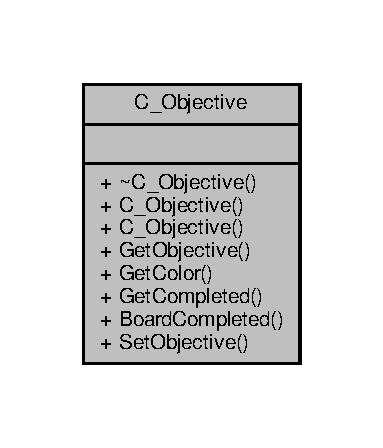
\includegraphics[width=184pt]{classC__Objective__coll__graph}
\end{center}
\end{figure}
\subsection*{Public Member Functions}
\begin{DoxyCompactItemize}
\item 
\hyperlink{classC__Objective_a4e05cb06acbee6d49734e2696cd419e9}{$\sim$\+C\+\_\+\+Objective} ()
\begin{DoxyCompactList}\small\item\em Class methods. \end{DoxyCompactList}\item 
\hyperlink{classC__Objective_aedbb7d27ece1f7894285398ae79ea588}{C\+\_\+\+Objective} (M\+L\+V\+\_\+\+Color color=M\+L\+V\+\_\+\+C\+O\+L\+O\+R\+\_\+\+G\+R\+A\+Y70)
\begin{DoxyCompactList}\small\item\em Constructor of an m\+Objective, default constructor. \end{DoxyCompactList}\item 
\hyperlink{classC__Objective_ae92eb6210a460fa7b551651584790ac8}{C\+\_\+\+Objective} (const std\+::vector$<$ std\+::shared\+\_\+ptr$<$ \hyperlink{classA__Shape}{A\+\_\+\+Shape} $>$$>$ \&objective, M\+L\+V\+\_\+\+Color color=M\+L\+V\+\_\+\+C\+O\+L\+O\+R\+\_\+\+G\+R\+A\+Y70)
\begin{DoxyCompactList}\small\item\em Constructor of an m\+Objective. \end{DoxyCompactList}\item 
std\+::vector$<$ std\+::shared\+\_\+ptr$<$ \hyperlink{classA__Shape}{A\+\_\+\+Shape} $>$ $>$ \hyperlink{classC__Objective_aa8e3dea19bd4578246b183d2bad2d475}{Get\+Objective} ()
\begin{DoxyCompactList}\small\item\em Get all shape of the m\+Objective. \end{DoxyCompactList}\item 
M\+L\+V\+\_\+\+Color \hyperlink{classC__Objective_aeaaa69ca15b1e1d8edbc3f1920399964}{Get\+Color} ()
\begin{DoxyCompactList}\small\item\em Get the m\+Color of an \hyperlink{classC__Objective}{C\+\_\+\+Objective}. \end{DoxyCompactList}\item 
double \hyperlink{classC__Objective_a026149982f0d62ea0a039a8b94bbaae0}{Get\+Completed} (const std\+::vector$<$ std\+::shared\+\_\+ptr$<$ \hyperlink{classA__Shape}{A\+\_\+\+Shape} $>$$>$ \&objective, const std\+::vector$<$ std\+::shared\+\_\+ptr$<$ \hyperlink{classA__Shape}{A\+\_\+\+Shape} $>$$>$ \&game)
\begin{DoxyCompactList}\small\item\em Give the progress of the puzzle. \end{DoxyCompactList}\item 
void \hyperlink{classC__Objective_a05924ace1e7f1c2f04de7f6c007cb104}{Clear} ()
\begin{DoxyCompactList}\small\item\em Clear the objective. \end{DoxyCompactList}\end{DoxyCompactItemize}
\subsection*{Static Public Member Functions}
\begin{DoxyCompactItemize}
\item 
static bool \hyperlink{classC__Objective_a5ad5b8ed6a640c86276d34c6a7a58346}{Board\+Completed} (const std\+::vector$<$ std\+::shared\+\_\+ptr$<$ \hyperlink{classA__Shape}{A\+\_\+\+Shape} $>$$>$ \&objective, const std\+::vector$<$ std\+::shared\+\_\+ptr$<$ \hyperlink{classA__Shape}{A\+\_\+\+Shape} $>$$>$ \&game)
\begin{DoxyCompactList}\small\item\em Check if the board is m\+Completed. \end{DoxyCompactList}\item 
static void \hyperlink{classC__Objective_a931d916840c73104815dbf529f9c866c}{Set\+Objective} (std\+::shared\+\_\+ptr$<$ \hyperlink{classC__Objective}{C\+\_\+\+Objective} $>$ objective, const std\+::vector$<$ std\+::shared\+\_\+ptr$<$ \hyperlink{classA__Shape}{A\+\_\+\+Shape} $>$$>$ \&vec\+\_\+objective)
\begin{DoxyCompactList}\small\item\em Set an \hyperlink{classC__Objective}{C\+\_\+\+Objective} for a new game. \end{DoxyCompactList}\end{DoxyCompactItemize}


\subsection{Detailed Description}
Class of the board \hyperlink{classC__Objective}{C\+\_\+\+Objective}. 

This class manage everything about the m\+Objective 

\subsection{Constructor \& Destructor Documentation}
\mbox{\Hypertarget{classC__Objective_a4e05cb06acbee6d49734e2696cd419e9}\label{classC__Objective_a4e05cb06acbee6d49734e2696cd419e9}} 
\index{C\+\_\+\+Objective@{C\+\_\+\+Objective}!````~C\+\_\+\+Objective@{$\sim$\+C\+\_\+\+Objective}}
\index{````~C\+\_\+\+Objective@{$\sim$\+C\+\_\+\+Objective}!C\+\_\+\+Objective@{C\+\_\+\+Objective}}
\subsubsection{\texorpdfstring{$\sim$\+C\+\_\+\+Objective()}{~C\_Objective()}}
{\footnotesize\ttfamily C\+\_\+\+Objective\+::$\sim$\+C\+\_\+\+Objective (\begin{DoxyParamCaption}{ }\end{DoxyParamCaption})}



Class methods. 

\mbox{\Hypertarget{classC__Objective_aedbb7d27ece1f7894285398ae79ea588}\label{classC__Objective_aedbb7d27ece1f7894285398ae79ea588}} 
\index{C\+\_\+\+Objective@{C\+\_\+\+Objective}!C\+\_\+\+Objective@{C\+\_\+\+Objective}}
\index{C\+\_\+\+Objective@{C\+\_\+\+Objective}!C\+\_\+\+Objective@{C\+\_\+\+Objective}}
\subsubsection{\texorpdfstring{C\+\_\+\+Objective()}{C\_Objective()}\hspace{0.1cm}{\footnotesize\ttfamily [1/2]}}
{\footnotesize\ttfamily C\+\_\+\+Objective\+::\+C\+\_\+\+Objective (\begin{DoxyParamCaption}\item[{M\+L\+V\+\_\+\+Color}]{color = {\ttfamily MLV\+\_\+COLOR\+\_\+GRAY70} }\end{DoxyParamCaption})\hspace{0.3cm}{\ttfamily [explicit]}}



Constructor of an m\+Objective, default constructor. 


\begin{DoxyParams}{Parameters}
{\em color} & \+: m\+Color of the m\+Objective shape \\
\hline
\end{DoxyParams}
\mbox{\Hypertarget{classC__Objective_ae92eb6210a460fa7b551651584790ac8}\label{classC__Objective_ae92eb6210a460fa7b551651584790ac8}} 
\index{C\+\_\+\+Objective@{C\+\_\+\+Objective}!C\+\_\+\+Objective@{C\+\_\+\+Objective}}
\index{C\+\_\+\+Objective@{C\+\_\+\+Objective}!C\+\_\+\+Objective@{C\+\_\+\+Objective}}
\subsubsection{\texorpdfstring{C\+\_\+\+Objective()}{C\_Objective()}\hspace{0.1cm}{\footnotesize\ttfamily [2/2]}}
{\footnotesize\ttfamily C\+\_\+\+Objective\+::\+C\+\_\+\+Objective (\begin{DoxyParamCaption}\item[{const std\+::vector$<$ std\+::shared\+\_\+ptr$<$ \hyperlink{classA__Shape}{A\+\_\+\+Shape} $>$$>$ \&}]{objective,  }\item[{M\+L\+V\+\_\+\+Color}]{color = {\ttfamily MLV\+\_\+COLOR\+\_\+GRAY70} }\end{DoxyParamCaption})\hspace{0.3cm}{\ttfamily [explicit]}}



Constructor of an m\+Objective. 


\begin{DoxyParams}{Parameters}
{\em objective} & \+: \hyperlink{classC__Objective}{C\+\_\+\+Objective} requires a vector of \hyperlink{classA__Shape}{A\+\_\+\+Shape} \\
\hline
{\em color} & \+: m\+Color of the m\+Objective shape \\
\hline
\end{DoxyParams}


\subsection{Member Function Documentation}
\mbox{\Hypertarget{classC__Objective_a5ad5b8ed6a640c86276d34c6a7a58346}\label{classC__Objective_a5ad5b8ed6a640c86276d34c6a7a58346}} 
\index{C\+\_\+\+Objective@{C\+\_\+\+Objective}!Board\+Completed@{Board\+Completed}}
\index{Board\+Completed@{Board\+Completed}!C\+\_\+\+Objective@{C\+\_\+\+Objective}}
\subsubsection{\texorpdfstring{Board\+Completed()}{BoardCompleted()}}
{\footnotesize\ttfamily bool C\+\_\+\+Objective\+::\+Board\+Completed (\begin{DoxyParamCaption}\item[{const std\+::vector$<$ std\+::shared\+\_\+ptr$<$ \hyperlink{classA__Shape}{A\+\_\+\+Shape} $>$$>$ \&}]{objective,  }\item[{const std\+::vector$<$ std\+::shared\+\_\+ptr$<$ \hyperlink{classA__Shape}{A\+\_\+\+Shape} $>$$>$ \&}]{game }\end{DoxyParamCaption})\hspace{0.3cm}{\ttfamily [static]}}



Check if the board is m\+Completed. 


\begin{DoxyParams}{Parameters}
{\em objective} & \+: Vector of m\+Objective\textquotesingle{}s shape \\
\hline
{\em game} & \+: Vector of current game\textquotesingle{}s shape \\
\hline
\end{DoxyParams}
\begin{DoxyReturn}{Returns}
True if the board is m\+Completed, false if not 
\end{DoxyReturn}
\mbox{\Hypertarget{classC__Objective_a05924ace1e7f1c2f04de7f6c007cb104}\label{classC__Objective_a05924ace1e7f1c2f04de7f6c007cb104}} 
\index{C\+\_\+\+Objective@{C\+\_\+\+Objective}!Clear@{Clear}}
\index{Clear@{Clear}!C\+\_\+\+Objective@{C\+\_\+\+Objective}}
\subsubsection{\texorpdfstring{Clear()}{Clear()}}
{\footnotesize\ttfamily void C\+\_\+\+Objective\+::\+Clear (\begin{DoxyParamCaption}{ }\end{DoxyParamCaption})}



Clear the objective. 

\mbox{\Hypertarget{classC__Objective_aeaaa69ca15b1e1d8edbc3f1920399964}\label{classC__Objective_aeaaa69ca15b1e1d8edbc3f1920399964}} 
\index{C\+\_\+\+Objective@{C\+\_\+\+Objective}!Get\+Color@{Get\+Color}}
\index{Get\+Color@{Get\+Color}!C\+\_\+\+Objective@{C\+\_\+\+Objective}}
\subsubsection{\texorpdfstring{Get\+Color()}{GetColor()}}
{\footnotesize\ttfamily M\+L\+V\+\_\+\+Color C\+\_\+\+Objective\+::\+Get\+Color (\begin{DoxyParamCaption}{ }\end{DoxyParamCaption})}



Get the m\+Color of an \hyperlink{classC__Objective}{C\+\_\+\+Objective}. 

\begin{DoxyReturn}{Returns}
Return the m\+Color of an \hyperlink{classC__Objective}{C\+\_\+\+Objective} 
\end{DoxyReturn}
\mbox{\Hypertarget{classC__Objective_a026149982f0d62ea0a039a8b94bbaae0}\label{classC__Objective_a026149982f0d62ea0a039a8b94bbaae0}} 
\index{C\+\_\+\+Objective@{C\+\_\+\+Objective}!Get\+Completed@{Get\+Completed}}
\index{Get\+Completed@{Get\+Completed}!C\+\_\+\+Objective@{C\+\_\+\+Objective}}
\subsubsection{\texorpdfstring{Get\+Completed()}{GetCompleted()}}
{\footnotesize\ttfamily double C\+\_\+\+Objective\+::\+Get\+Completed (\begin{DoxyParamCaption}\item[{const std\+::vector$<$ std\+::shared\+\_\+ptr$<$ \hyperlink{classA__Shape}{A\+\_\+\+Shape} $>$$>$ \&}]{objective,  }\item[{const std\+::vector$<$ std\+::shared\+\_\+ptr$<$ \hyperlink{classA__Shape}{A\+\_\+\+Shape} $>$$>$ \&}]{game }\end{DoxyParamCaption})}



Give the progress of the puzzle. 


\begin{DoxyParams}{Parameters}
{\em objective} & \+: Shapes of objective \\
\hline
{\em game} & \+: Shape of the game \\
\hline
\end{DoxyParams}
\begin{DoxyReturn}{Returns}
Return the \%100 of the progress 
\end{DoxyReturn}
\mbox{\Hypertarget{classC__Objective_aa8e3dea19bd4578246b183d2bad2d475}\label{classC__Objective_aa8e3dea19bd4578246b183d2bad2d475}} 
\index{C\+\_\+\+Objective@{C\+\_\+\+Objective}!Get\+Objective@{Get\+Objective}}
\index{Get\+Objective@{Get\+Objective}!C\+\_\+\+Objective@{C\+\_\+\+Objective}}
\subsubsection{\texorpdfstring{Get\+Objective()}{GetObjective()}}
{\footnotesize\ttfamily std\+::vector$<$ std\+::shared\+\_\+ptr$<$ \hyperlink{classA__Shape}{A\+\_\+\+Shape} $>$ $>$ C\+\_\+\+Objective\+::\+Get\+Objective (\begin{DoxyParamCaption}{ }\end{DoxyParamCaption})}



Get all shape of the m\+Objective. 

\begin{DoxyReturn}{Returns}
Return a vector of shape of the m\+Objective 
\end{DoxyReturn}
\mbox{\Hypertarget{classC__Objective_a931d916840c73104815dbf529f9c866c}\label{classC__Objective_a931d916840c73104815dbf529f9c866c}} 
\index{C\+\_\+\+Objective@{C\+\_\+\+Objective}!Set\+Objective@{Set\+Objective}}
\index{Set\+Objective@{Set\+Objective}!C\+\_\+\+Objective@{C\+\_\+\+Objective}}
\subsubsection{\texorpdfstring{Set\+Objective()}{SetObjective()}}
{\footnotesize\ttfamily void C\+\_\+\+Objective\+::\+Set\+Objective (\begin{DoxyParamCaption}\item[{std\+::shared\+\_\+ptr$<$ \hyperlink{classC__Objective}{C\+\_\+\+Objective} $>$}]{objective,  }\item[{const std\+::vector$<$ std\+::shared\+\_\+ptr$<$ \hyperlink{classA__Shape}{A\+\_\+\+Shape} $>$$>$ \&}]{vec\+\_\+objective }\end{DoxyParamCaption})\hspace{0.3cm}{\ttfamily [static]}}



Set an \hyperlink{classC__Objective}{C\+\_\+\+Objective} for a new game. 


\begin{DoxyParams}{Parameters}
{\em objective} & \+: \hyperlink{classC__Objective}{C\+\_\+\+Objective} to m\+Update \\
\hline
{\em vec\+\_\+objective} & \+:Vector of new \hyperlink{classA__Shape}{A\+\_\+\+Shape} for the new \hyperlink{classC__Objective}{C\+\_\+\+Objective} \\
\hline
\end{DoxyParams}


The documentation for this class was generated from the following files\+:\begin{DoxyCompactItemize}
\item 
include/game/\hyperlink{C__Objective_8hpp}{C\+\_\+\+Objective.\+hpp}\item 
src/game/\hyperlink{C__Objective_8cpp}{C\+\_\+\+Objective.\+cpp}\end{DoxyCompactItemize}

\hypertarget{classC__Parallelogram}{}\section{C\+\_\+\+Parallelogram Class Reference}
\label{classC__Parallelogram}\index{C\+\_\+\+Parallelogram@{C\+\_\+\+Parallelogram}}


Class of the parallelogram.  




{\ttfamily \#include $<$C\+\_\+\+Parallelogram.\+hpp$>$}



Inheritance diagram for C\+\_\+\+Parallelogram\+:
\nopagebreak
\begin{figure}[H]
\begin{center}
\leavevmode
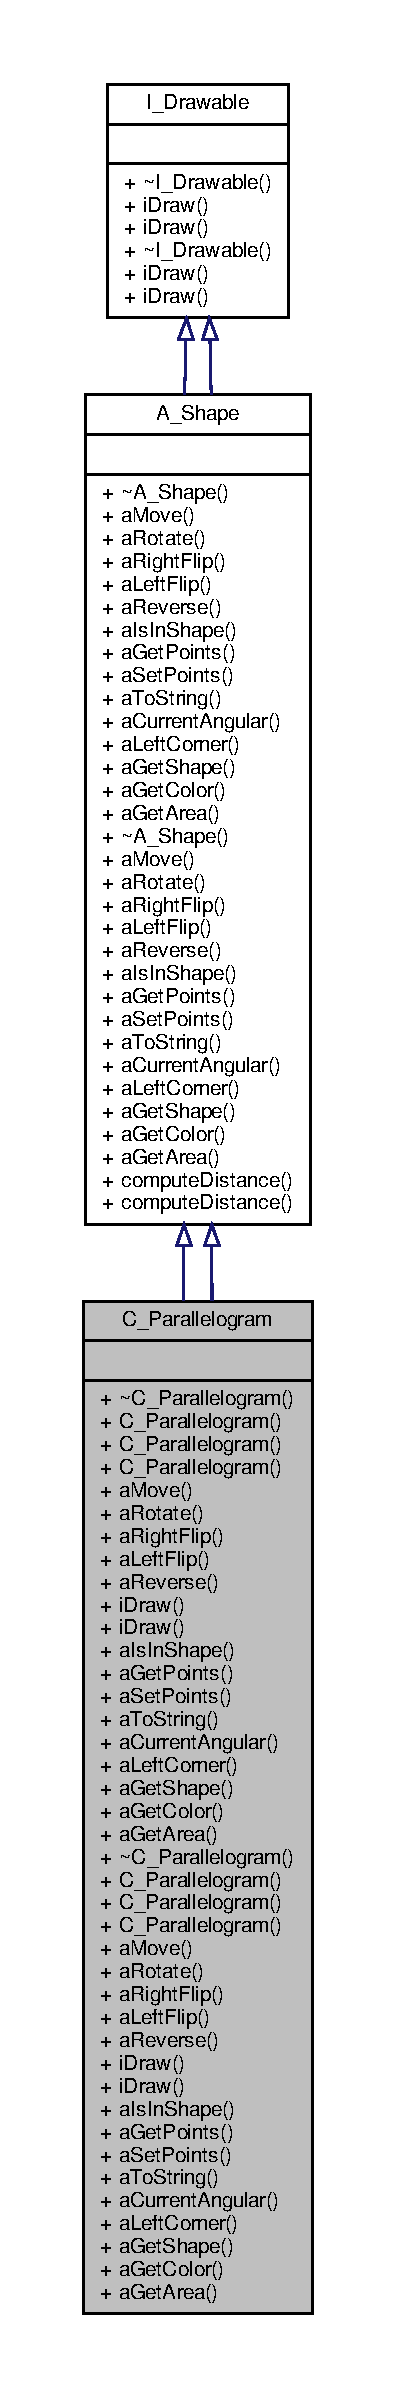
\includegraphics[height=550pt]{classC__Parallelogram__inherit__graph}
\end{center}
\end{figure}


Collaboration diagram for C\+\_\+\+Parallelogram\+:
\nopagebreak
\begin{figure}[H]
\begin{center}
\leavevmode
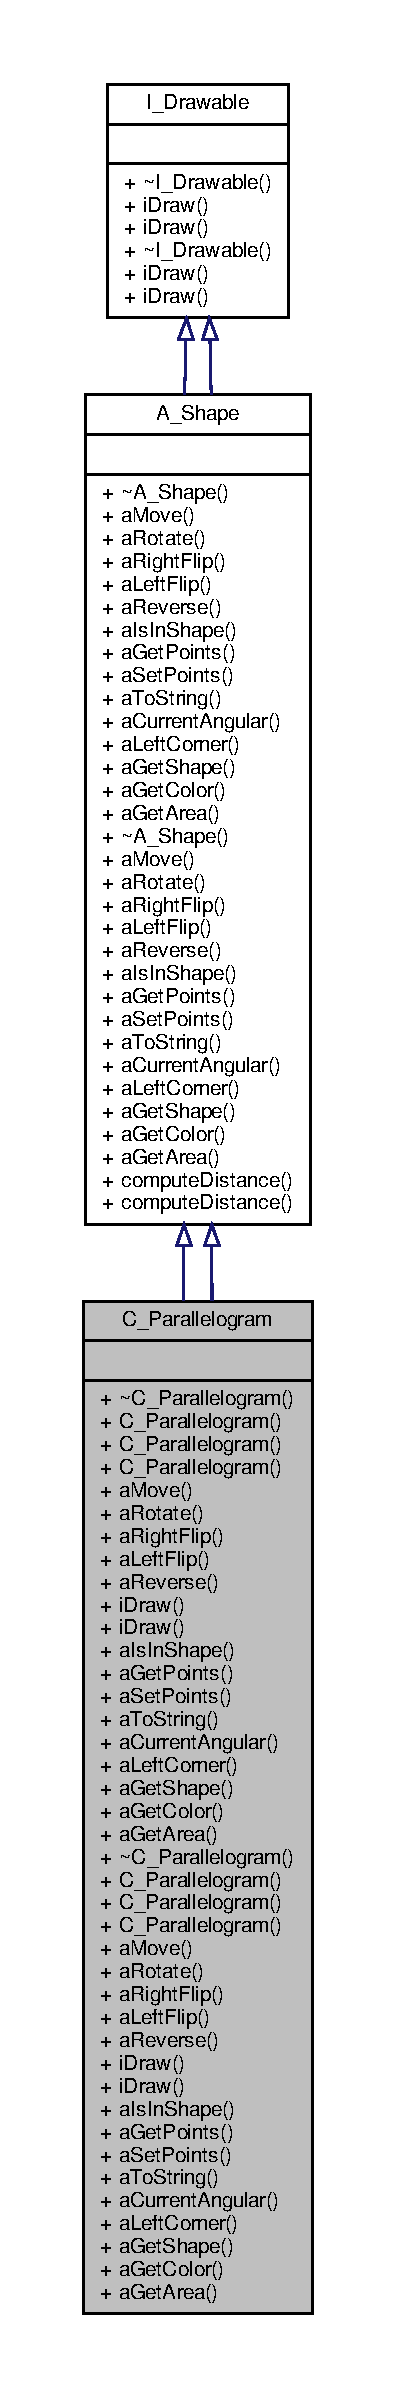
\includegraphics[height=550pt]{classC__Parallelogram__coll__graph}
\end{center}
\end{figure}
\subsection*{Public Member Functions}
\begin{DoxyCompactItemize}
\item 
\hyperlink{classC__Parallelogram_a2d7af48f3a26e8e07031e7c147a084a3}{$\sim$\+C\+\_\+\+Parallelogram} () override
\begin{DoxyCompactList}\small\item\em Destructor of \hyperlink{classC__Parallelogram}{C\+\_\+\+Parallelogram}. \end{DoxyCompactList}\item 
\hyperlink{classC__Parallelogram_a85d543d3a3a118676e7e47cff7ce82be}{C\+\_\+\+Parallelogram} (M\+L\+V\+\_\+\+Color color=M\+L\+V\+\_\+\+C\+O\+L\+O\+R\+\_\+\+B\+L\+UE)
\begin{DoxyCompactList}\small\item\em Constructor by default of \hyperlink{classC__Parallelogram}{C\+\_\+\+Parallelogram}, make a \hyperlink{classC__Parallelogram}{C\+\_\+\+Parallelogram} as default. \end{DoxyCompactList}\item 
\hyperlink{classC__Parallelogram_a6e31f5dcaf076ca4b745c0b0108bb809}{C\+\_\+\+Parallelogram} (const std\+::vector$<$ \hyperlink{classC__STriangle}{C\+\_\+\+S\+Triangle} $>$ \&triangle, M\+L\+V\+\_\+\+Color color=M\+L\+V\+\_\+\+C\+O\+L\+O\+R\+\_\+\+B\+L\+UE)
\begin{DoxyCompactList}\small\item\em Constructor of \hyperlink{classC__Parallelogram}{C\+\_\+\+Parallelogram}, requires a vector of S\+Triangles. \end{DoxyCompactList}\item 
\hyperlink{classC__Parallelogram_abd470868efc5d3a002509a9e45e4ed63}{C\+\_\+\+Parallelogram} (const \hyperlink{classT__Point}{T\+\_\+\+Point}$<$ double $>$ \&origin, double angular=0.\+0, M\+L\+V\+\_\+\+Color color=M\+L\+V\+\_\+\+C\+O\+L\+O\+R\+\_\+\+B\+L\+UE)
\begin{DoxyCompactList}\small\item\em Constructor of \hyperlink{classC__Parallelogram}{C\+\_\+\+Parallelogram}, calls the deleguate Default Constructor. \end{DoxyCompactList}\item 
void \hyperlink{classC__Parallelogram_ac77ea776b24c551114d84eaf147f6977}{a\+Move} (const \hyperlink{classT__Point}{T\+\_\+\+Point}$<$ double $>$ \&translation) override
\begin{DoxyCompactList}\small\item\em Move the \hyperlink{classC__Parallelogram}{C\+\_\+\+Parallelogram} by point translation. \end{DoxyCompactList}\item 
void \hyperlink{classC__Parallelogram_a07b6dfae7100a409cdcf04d710ac9c3f}{a\+Rotate} (double angular) override
\begin{DoxyCompactList}\small\item\em Rotate the \hyperlink{classC__Parallelogram}{C\+\_\+\+Parallelogram} with specified angular. \end{DoxyCompactList}\item 
void \hyperlink{classC__Parallelogram_ab638d55c999ea10da7b5000fd034fbc1}{a\+Right\+Flip} () override
\begin{DoxyCompactList}\small\item\em Flip the figure as 45° clock. \end{DoxyCompactList}\item 
void \hyperlink{classC__Parallelogram_a284a59c9f1c778ac8da80efedc313354}{a\+Left\+Flip} () override
\begin{DoxyCompactList}\small\item\em Flip the figure as 45° anti clock. \end{DoxyCompactList}\item 
void \hyperlink{classC__Parallelogram_a573447294989d53fadf3d7adfb0640c6}{a\+Reverse} () override
\begin{DoxyCompactList}\small\item\em Reverse the figure as symmetry. \end{DoxyCompactList}\item 
void \hyperlink{classC__Parallelogram_a6d43cc787a39def68c7b7de4a33caf5e}{i\+Draw} () override
\begin{DoxyCompactList}\small\item\em Draw this shape on I\+HM. \end{DoxyCompactList}\item 
void \hyperlink{classC__Parallelogram_a044ce6d1042ea93589a38f4686489862}{i\+Draw} (M\+L\+V\+\_\+\+Color color) override
\begin{DoxyCompactList}\small\item\em Draw this shape on I\+HM with specific color. \end{DoxyCompactList}\item 
bool \hyperlink{classC__Parallelogram_a9ccee396c30606bfe64df416c22586d5}{a\+Is\+In\+Shape} (const \hyperlink{classT__Point}{T\+\_\+\+Point}$<$ double $>$ \&click) override
\begin{DoxyCompactList}\small\item\em Check if a point is in this shape. \end{DoxyCompactList}\item 
std\+::vector$<$ \hyperlink{classT__Point}{T\+\_\+\+Point}$<$ double $>$ $>$ \hyperlink{classC__Parallelogram_ae75f316315134020e8423feff917828e}{a\+Get\+Points} () override
\begin{DoxyCompactList}\small\item\em Get m\+Points of this shape. \end{DoxyCompactList}\item 
bool \hyperlink{classC__Parallelogram_adfe1c40f2d33955617e3a535c548dfa0}{a\+Set\+Points} (const \hyperlink{classT__Point}{T\+\_\+\+Point}$<$ double $>$ \&ref, const \hyperlink{classT__Point}{T\+\_\+\+Point}$<$ double $>$ \&changed) override
\begin{DoxyCompactList}\small\item\em Set a point to another one. \end{DoxyCompactList}\item 
std\+::string \hyperlink{classC__Parallelogram_add67ef2aba5e14c27e30a958e4843223}{a\+To\+String} () override
\begin{DoxyCompactList}\small\item\em Convert all data of \hyperlink{classC__Parallelogram}{C\+\_\+\+Parallelogram} in a string. \end{DoxyCompactList}\item 
double \hyperlink{classC__Parallelogram_a51959da2b0cf083767f39d8065f395f2}{a\+Current\+Angular} () override
\begin{DoxyCompactList}\small\item\em Get the current angular of this shape. \end{DoxyCompactList}\item 
\hyperlink{classT__Point}{T\+\_\+\+Point}$<$ double $>$ \hyperlink{classC__Parallelogram_a260c557810c63dd97f2dd64bc15b9dc8}{a\+Left\+Corner} () override
\begin{DoxyCompactList}\small\item\em Take the point at left top corner. \end{DoxyCompactList}\item 
std\+::string \hyperlink{classC__Parallelogram_a373fdd3ebdfeffcaa0a72ff7001af8ec}{a\+Get\+Shape} () override
\begin{DoxyCompactList}\small\item\em Get the shape type. \end{DoxyCompactList}\item 
M\+L\+V\+\_\+\+Color \hyperlink{classC__Parallelogram_afd5055e948fcd992be3cdd227c8b4bfb}{a\+Get\+Color} () override
\begin{DoxyCompactList}\small\item\em Get the color of the shape. \end{DoxyCompactList}\item 
double \hyperlink{classC__Parallelogram_a72b4509a33ee27331e5b9bdc8a3278e8}{a\+Get\+Area} () override
\begin{DoxyCompactList}\small\item\em Get the area of the shape. \end{DoxyCompactList}\end{DoxyCompactItemize}
\subsection*{Additional Inherited Members}


\subsection{Detailed Description}
Class of the parallelogram. 

This class manage everything about the \hyperlink{classC__Parallelogram}{C\+\_\+\+Parallelogram} 

\subsection{Constructor \& Destructor Documentation}
\mbox{\Hypertarget{classC__Parallelogram_a2d7af48f3a26e8e07031e7c147a084a3}\label{classC__Parallelogram_a2d7af48f3a26e8e07031e7c147a084a3}} 
\index{C\+\_\+\+Parallelogram@{C\+\_\+\+Parallelogram}!````~C\+\_\+\+Parallelogram@{$\sim$\+C\+\_\+\+Parallelogram}}
\index{````~C\+\_\+\+Parallelogram@{$\sim$\+C\+\_\+\+Parallelogram}!C\+\_\+\+Parallelogram@{C\+\_\+\+Parallelogram}}
\subsubsection{\texorpdfstring{$\sim$\+C\+\_\+\+Parallelogram()}{~C\_Parallelogram()}}
{\footnotesize\ttfamily C\+\_\+\+Parallelogram\+::$\sim$\+C\+\_\+\+Parallelogram (\begin{DoxyParamCaption}{ }\end{DoxyParamCaption})\hspace{0.3cm}{\ttfamily [override]}}



Destructor of \hyperlink{classC__Parallelogram}{C\+\_\+\+Parallelogram}. 

\mbox{\Hypertarget{classC__Parallelogram_a85d543d3a3a118676e7e47cff7ce82be}\label{classC__Parallelogram_a85d543d3a3a118676e7e47cff7ce82be}} 
\index{C\+\_\+\+Parallelogram@{C\+\_\+\+Parallelogram}!C\+\_\+\+Parallelogram@{C\+\_\+\+Parallelogram}}
\index{C\+\_\+\+Parallelogram@{C\+\_\+\+Parallelogram}!C\+\_\+\+Parallelogram@{C\+\_\+\+Parallelogram}}
\subsubsection{\texorpdfstring{C\+\_\+\+Parallelogram()}{C\_Parallelogram()}\hspace{0.1cm}{\footnotesize\ttfamily [1/3]}}
{\footnotesize\ttfamily C\+\_\+\+Parallelogram\+::\+C\+\_\+\+Parallelogram (\begin{DoxyParamCaption}\item[{M\+L\+V\+\_\+\+Color}]{color = {\ttfamily MLV\+\_\+COLOR\+\_\+BLUE} }\end{DoxyParamCaption})\hspace{0.3cm}{\ttfamily [explicit]}}



Constructor by default of \hyperlink{classC__Parallelogram}{C\+\_\+\+Parallelogram}, make a \hyperlink{classC__Parallelogram}{C\+\_\+\+Parallelogram} as default. 


\begin{DoxyParams}{Parameters}
{\em color} & \+: Optional \+\_\+\+\_\+\+Parameter, m\+Color of this shape \\
\hline
\end{DoxyParams}
\mbox{\Hypertarget{classC__Parallelogram_a6e31f5dcaf076ca4b745c0b0108bb809}\label{classC__Parallelogram_a6e31f5dcaf076ca4b745c0b0108bb809}} 
\index{C\+\_\+\+Parallelogram@{C\+\_\+\+Parallelogram}!C\+\_\+\+Parallelogram@{C\+\_\+\+Parallelogram}}
\index{C\+\_\+\+Parallelogram@{C\+\_\+\+Parallelogram}!C\+\_\+\+Parallelogram@{C\+\_\+\+Parallelogram}}
\subsubsection{\texorpdfstring{C\+\_\+\+Parallelogram()}{C\_Parallelogram()}\hspace{0.1cm}{\footnotesize\ttfamily [2/3]}}
{\footnotesize\ttfamily C\+\_\+\+Parallelogram\+::\+C\+\_\+\+Parallelogram (\begin{DoxyParamCaption}\item[{const std\+::vector$<$ \hyperlink{classC__STriangle}{C\+\_\+\+S\+Triangle} $>$ \&}]{triangle,  }\item[{M\+L\+V\+\_\+\+Color}]{color = {\ttfamily MLV\+\_\+COLOR\+\_\+BLUE} }\end{DoxyParamCaption})\hspace{0.3cm}{\ttfamily [explicit]}}



Constructor of \hyperlink{classC__Parallelogram}{C\+\_\+\+Parallelogram}, requires a vector of S\+Triangles. 


\begin{DoxyParams}{Parameters}
{\em triangle} & \+: The \hyperlink{classC__Parallelogram}{C\+\_\+\+Parallelogram} will created with a vector of \hyperlink{classC__STriangle}{C\+\_\+\+S\+Triangle} (4) \\
\hline
{\em color} & \+: Optional \+\_\+\+\_\+\+Parameter, m\+Color of this shape \\
\hline
\end{DoxyParams}
\mbox{\Hypertarget{classC__Parallelogram_abd470868efc5d3a002509a9e45e4ed63}\label{classC__Parallelogram_abd470868efc5d3a002509a9e45e4ed63}} 
\index{C\+\_\+\+Parallelogram@{C\+\_\+\+Parallelogram}!C\+\_\+\+Parallelogram@{C\+\_\+\+Parallelogram}}
\index{C\+\_\+\+Parallelogram@{C\+\_\+\+Parallelogram}!C\+\_\+\+Parallelogram@{C\+\_\+\+Parallelogram}}
\subsubsection{\texorpdfstring{C\+\_\+\+Parallelogram()}{C\_Parallelogram()}\hspace{0.1cm}{\footnotesize\ttfamily [3/3]}}
{\footnotesize\ttfamily C\+\_\+\+Parallelogram\+::\+C\+\_\+\+Parallelogram (\begin{DoxyParamCaption}\item[{const \hyperlink{classT__Point}{T\+\_\+\+Point}$<$ double $>$ \&}]{origin,  }\item[{double}]{angular = {\ttfamily 0.0},  }\item[{M\+L\+V\+\_\+\+Color}]{color = {\ttfamily MLV\+\_\+COLOR\+\_\+BLUE} }\end{DoxyParamCaption})\hspace{0.3cm}{\ttfamily [explicit]}}



Constructor of \hyperlink{classC__Parallelogram}{C\+\_\+\+Parallelogram}, calls the deleguate Default Constructor. 


\begin{DoxyParams}{Parameters}
{\em origin} & \+: shifts the figure of a translation of the origin \\
\hline
{\em angular} & \+: Optional \+\_\+\+\_\+\+Parameter (angular=0.\+0 as default), a\+Rotate the figure with an angular \\
\hline
{\em color} & \+: Optional \+\_\+\+\_\+\+Parameter, m\+Color of this shape \\
\hline
\end{DoxyParams}


\subsection{Member Function Documentation}
\mbox{\Hypertarget{classC__Parallelogram_a51959da2b0cf083767f39d8065f395f2}\label{classC__Parallelogram_a51959da2b0cf083767f39d8065f395f2}} 
\index{C\+\_\+\+Parallelogram@{C\+\_\+\+Parallelogram}!a\+Current\+Angular@{a\+Current\+Angular}}
\index{a\+Current\+Angular@{a\+Current\+Angular}!C\+\_\+\+Parallelogram@{C\+\_\+\+Parallelogram}}
\subsubsection{\texorpdfstring{a\+Current\+Angular()}{aCurrentAngular()}}
{\footnotesize\ttfamily double C\+\_\+\+Parallelogram\+::a\+Current\+Angular (\begin{DoxyParamCaption}{ }\end{DoxyParamCaption})\hspace{0.3cm}{\ttfamily [override]}, {\ttfamily [virtual]}}



Get the current angular of this shape. 

\begin{DoxyReturn}{Returns}

\end{DoxyReturn}


Implements \hyperlink{classA__Shape_a80fa4e009c875dd0ba7fc5bfeeb43f98}{A\+\_\+\+Shape}.

\mbox{\Hypertarget{classC__Parallelogram_a72b4509a33ee27331e5b9bdc8a3278e8}\label{classC__Parallelogram_a72b4509a33ee27331e5b9bdc8a3278e8}} 
\index{C\+\_\+\+Parallelogram@{C\+\_\+\+Parallelogram}!a\+Get\+Area@{a\+Get\+Area}}
\index{a\+Get\+Area@{a\+Get\+Area}!C\+\_\+\+Parallelogram@{C\+\_\+\+Parallelogram}}
\subsubsection{\texorpdfstring{a\+Get\+Area()}{aGetArea()}}
{\footnotesize\ttfamily double C\+\_\+\+Parallelogram\+::a\+Get\+Area (\begin{DoxyParamCaption}{ }\end{DoxyParamCaption})\hspace{0.3cm}{\ttfamily [override]}, {\ttfamily [virtual]}}



Get the area of the shape. 

\begin{DoxyReturn}{Returns}
Return the area of the shape 
\end{DoxyReturn}


Implements \hyperlink{classA__Shape_a1b142ee2d873d6c217f65de1632e7b6e}{A\+\_\+\+Shape}.

\mbox{\Hypertarget{classC__Parallelogram_afd5055e948fcd992be3cdd227c8b4bfb}\label{classC__Parallelogram_afd5055e948fcd992be3cdd227c8b4bfb}} 
\index{C\+\_\+\+Parallelogram@{C\+\_\+\+Parallelogram}!a\+Get\+Color@{a\+Get\+Color}}
\index{a\+Get\+Color@{a\+Get\+Color}!C\+\_\+\+Parallelogram@{C\+\_\+\+Parallelogram}}
\subsubsection{\texorpdfstring{a\+Get\+Color()}{aGetColor()}}
{\footnotesize\ttfamily M\+L\+V\+\_\+\+Color C\+\_\+\+Parallelogram\+::a\+Get\+Color (\begin{DoxyParamCaption}{ }\end{DoxyParamCaption})\hspace{0.3cm}{\ttfamily [override]}, {\ttfamily [virtual]}}



Get the color of the shape. 

\begin{DoxyReturn}{Returns}
Return the M\+L\+V\+\_\+\+Color of the shape 
\end{DoxyReturn}


Implements \hyperlink{classA__Shape_a1e90c8132d33e4ac84d42f72606193b2}{A\+\_\+\+Shape}.

\mbox{\Hypertarget{classC__Parallelogram_ae75f316315134020e8423feff917828e}\label{classC__Parallelogram_ae75f316315134020e8423feff917828e}} 
\index{C\+\_\+\+Parallelogram@{C\+\_\+\+Parallelogram}!a\+Get\+Points@{a\+Get\+Points}}
\index{a\+Get\+Points@{a\+Get\+Points}!C\+\_\+\+Parallelogram@{C\+\_\+\+Parallelogram}}
\subsubsection{\texorpdfstring{a\+Get\+Points()}{aGetPoints()}}
{\footnotesize\ttfamily std\+::vector$<$ \hyperlink{classT__Point}{T\+\_\+\+Point}$<$ double $>$ $>$ C\+\_\+\+Parallelogram\+::a\+Get\+Points (\begin{DoxyParamCaption}{ }\end{DoxyParamCaption})\hspace{0.3cm}{\ttfamily [override]}, {\ttfamily [virtual]}}



Get m\+Points of this shape. 

\begin{DoxyReturn}{Returns}
Return a vector of m\+Points of this shape 
\end{DoxyReturn}


Implements \hyperlink{classA__Shape_a9fd1285bd63b1fc88943c9969bf01a5c}{A\+\_\+\+Shape}.

\mbox{\Hypertarget{classC__Parallelogram_a373fdd3ebdfeffcaa0a72ff7001af8ec}\label{classC__Parallelogram_a373fdd3ebdfeffcaa0a72ff7001af8ec}} 
\index{C\+\_\+\+Parallelogram@{C\+\_\+\+Parallelogram}!a\+Get\+Shape@{a\+Get\+Shape}}
\index{a\+Get\+Shape@{a\+Get\+Shape}!C\+\_\+\+Parallelogram@{C\+\_\+\+Parallelogram}}
\subsubsection{\texorpdfstring{a\+Get\+Shape()}{aGetShape()}}
{\footnotesize\ttfamily std\+::string C\+\_\+\+Parallelogram\+::a\+Get\+Shape (\begin{DoxyParamCaption}{ }\end{DoxyParamCaption})\hspace{0.3cm}{\ttfamily [override]}, {\ttfamily [virtual]}}



Get the shape type. 

\begin{DoxyReturn}{Returns}
Return as string the shape type 
\end{DoxyReturn}


Implements \hyperlink{classA__Shape_a1b202256a4e5dcb0edab4ab93a37122c}{A\+\_\+\+Shape}.

\mbox{\Hypertarget{classC__Parallelogram_a9ccee396c30606bfe64df416c22586d5}\label{classC__Parallelogram_a9ccee396c30606bfe64df416c22586d5}} 
\index{C\+\_\+\+Parallelogram@{C\+\_\+\+Parallelogram}!a\+Is\+In\+Shape@{a\+Is\+In\+Shape}}
\index{a\+Is\+In\+Shape@{a\+Is\+In\+Shape}!C\+\_\+\+Parallelogram@{C\+\_\+\+Parallelogram}}
\subsubsection{\texorpdfstring{a\+Is\+In\+Shape()}{aIsInShape()}}
{\footnotesize\ttfamily bool C\+\_\+\+Parallelogram\+::a\+Is\+In\+Shape (\begin{DoxyParamCaption}\item[{const \hyperlink{classT__Point}{T\+\_\+\+Point}$<$ double $>$ \&}]{click }\end{DoxyParamCaption})\hspace{0.3cm}{\ttfamily [override]}, {\ttfamily [virtual]}}



Check if a point is in this shape. 


\begin{DoxyParams}{Parameters}
{\em click} & \+: \hyperlink{classT__Point}{T\+\_\+\+Point} to check \\
\hline
\end{DoxyParams}
\begin{DoxyReturn}{Returns}
true if Click is in this shape, false if not 
\end{DoxyReturn}


Implements \hyperlink{classA__Shape_a63f825cbc9780208d9a137f5c14917d0}{A\+\_\+\+Shape}.

\mbox{\Hypertarget{classC__Parallelogram_a260c557810c63dd97f2dd64bc15b9dc8}\label{classC__Parallelogram_a260c557810c63dd97f2dd64bc15b9dc8}} 
\index{C\+\_\+\+Parallelogram@{C\+\_\+\+Parallelogram}!a\+Left\+Corner@{a\+Left\+Corner}}
\index{a\+Left\+Corner@{a\+Left\+Corner}!C\+\_\+\+Parallelogram@{C\+\_\+\+Parallelogram}}
\subsubsection{\texorpdfstring{a\+Left\+Corner()}{aLeftCorner()}}
{\footnotesize\ttfamily \hyperlink{classT__Point}{T\+\_\+\+Point}$<$ double $>$ C\+\_\+\+Parallelogram\+::a\+Left\+Corner (\begin{DoxyParamCaption}{ }\end{DoxyParamCaption})\hspace{0.3cm}{\ttfamily [override]}, {\ttfamily [virtual]}}



Take the point at left top corner. 

\begin{DoxyReturn}{Returns}
Return the point at left top corner 
\end{DoxyReturn}


Implements \hyperlink{classA__Shape_abe6781b13037bf7ecea8ff9456b31533}{A\+\_\+\+Shape}.

\mbox{\Hypertarget{classC__Parallelogram_a284a59c9f1c778ac8da80efedc313354}\label{classC__Parallelogram_a284a59c9f1c778ac8da80efedc313354}} 
\index{C\+\_\+\+Parallelogram@{C\+\_\+\+Parallelogram}!a\+Left\+Flip@{a\+Left\+Flip}}
\index{a\+Left\+Flip@{a\+Left\+Flip}!C\+\_\+\+Parallelogram@{C\+\_\+\+Parallelogram}}
\subsubsection{\texorpdfstring{a\+Left\+Flip()}{aLeftFlip()}}
{\footnotesize\ttfamily void C\+\_\+\+Parallelogram\+::a\+Left\+Flip (\begin{DoxyParamCaption}{ }\end{DoxyParamCaption})\hspace{0.3cm}{\ttfamily [override]}, {\ttfamily [virtual]}}



Flip the figure as 45° anti clock. 



Implements \hyperlink{classA__Shape_abe947e7003cb63be2b4f6c439533427d}{A\+\_\+\+Shape}.

\mbox{\Hypertarget{classC__Parallelogram_ac77ea776b24c551114d84eaf147f6977}\label{classC__Parallelogram_ac77ea776b24c551114d84eaf147f6977}} 
\index{C\+\_\+\+Parallelogram@{C\+\_\+\+Parallelogram}!a\+Move@{a\+Move}}
\index{a\+Move@{a\+Move}!C\+\_\+\+Parallelogram@{C\+\_\+\+Parallelogram}}
\subsubsection{\texorpdfstring{a\+Move()}{aMove()}}
{\footnotesize\ttfamily void C\+\_\+\+Parallelogram\+::a\+Move (\begin{DoxyParamCaption}\item[{const \hyperlink{classT__Point}{T\+\_\+\+Point}$<$ double $>$ \&}]{translation }\end{DoxyParamCaption})\hspace{0.3cm}{\ttfamily [override]}, {\ttfamily [virtual]}}



Move the \hyperlink{classC__Parallelogram}{C\+\_\+\+Parallelogram} by point translation. 


\begin{DoxyParams}{Parameters}
{\em translation} & \+: Every m\+Points of this shape will be translate by this \+\_\+\+\_\+\+Parameter \\
\hline
\end{DoxyParams}


Implements \hyperlink{classA__Shape_ab284298db1b557ccfa7ba6de7a5fee2c}{A\+\_\+\+Shape}.

\mbox{\Hypertarget{classC__Parallelogram_a573447294989d53fadf3d7adfb0640c6}\label{classC__Parallelogram_a573447294989d53fadf3d7adfb0640c6}} 
\index{C\+\_\+\+Parallelogram@{C\+\_\+\+Parallelogram}!a\+Reverse@{a\+Reverse}}
\index{a\+Reverse@{a\+Reverse}!C\+\_\+\+Parallelogram@{C\+\_\+\+Parallelogram}}
\subsubsection{\texorpdfstring{a\+Reverse()}{aReverse()}}
{\footnotesize\ttfamily void C\+\_\+\+Parallelogram\+::a\+Reverse (\begin{DoxyParamCaption}{ }\end{DoxyParamCaption})\hspace{0.3cm}{\ttfamily [override]}, {\ttfamily [virtual]}}



Reverse the figure as symmetry. 



Implements \hyperlink{classA__Shape_afe2c7969d647f6358da13879a7534ecb}{A\+\_\+\+Shape}.

\mbox{\Hypertarget{classC__Parallelogram_ab638d55c999ea10da7b5000fd034fbc1}\label{classC__Parallelogram_ab638d55c999ea10da7b5000fd034fbc1}} 
\index{C\+\_\+\+Parallelogram@{C\+\_\+\+Parallelogram}!a\+Right\+Flip@{a\+Right\+Flip}}
\index{a\+Right\+Flip@{a\+Right\+Flip}!C\+\_\+\+Parallelogram@{C\+\_\+\+Parallelogram}}
\subsubsection{\texorpdfstring{a\+Right\+Flip()}{aRightFlip()}}
{\footnotesize\ttfamily void C\+\_\+\+Parallelogram\+::a\+Right\+Flip (\begin{DoxyParamCaption}{ }\end{DoxyParamCaption})\hspace{0.3cm}{\ttfamily [override]}, {\ttfamily [virtual]}}



Flip the figure as 45° clock. 



Implements \hyperlink{classA__Shape_a892688cbbad3297e00e87cce0dbfc76d}{A\+\_\+\+Shape}.

\mbox{\Hypertarget{classC__Parallelogram_a07b6dfae7100a409cdcf04d710ac9c3f}\label{classC__Parallelogram_a07b6dfae7100a409cdcf04d710ac9c3f}} 
\index{C\+\_\+\+Parallelogram@{C\+\_\+\+Parallelogram}!a\+Rotate@{a\+Rotate}}
\index{a\+Rotate@{a\+Rotate}!C\+\_\+\+Parallelogram@{C\+\_\+\+Parallelogram}}
\subsubsection{\texorpdfstring{a\+Rotate()}{aRotate()}}
{\footnotesize\ttfamily void C\+\_\+\+Parallelogram\+::a\+Rotate (\begin{DoxyParamCaption}\item[{double}]{angular }\end{DoxyParamCaption})\hspace{0.3cm}{\ttfamily [override]}, {\ttfamily [virtual]}}



Rotate the \hyperlink{classC__Parallelogram}{C\+\_\+\+Parallelogram} with specified angular. 


\begin{DoxyParams}{Parameters}
{\em angular} & \+: This angular should be between (0, 2\+PI) \\
\hline
\end{DoxyParams}


Implements \hyperlink{classA__Shape_a25b4e0c34cdb46da5382fe9c7467efaf}{A\+\_\+\+Shape}.

\mbox{\Hypertarget{classC__Parallelogram_adfe1c40f2d33955617e3a535c548dfa0}\label{classC__Parallelogram_adfe1c40f2d33955617e3a535c548dfa0}} 
\index{C\+\_\+\+Parallelogram@{C\+\_\+\+Parallelogram}!a\+Set\+Points@{a\+Set\+Points}}
\index{a\+Set\+Points@{a\+Set\+Points}!C\+\_\+\+Parallelogram@{C\+\_\+\+Parallelogram}}
\subsubsection{\texorpdfstring{a\+Set\+Points()}{aSetPoints()}}
{\footnotesize\ttfamily bool C\+\_\+\+Parallelogram\+::a\+Set\+Points (\begin{DoxyParamCaption}\item[{const \hyperlink{classT__Point}{T\+\_\+\+Point}$<$ double $>$ \&}]{ref,  }\item[{const \hyperlink{classT__Point}{T\+\_\+\+Point}$<$ double $>$ \&}]{changed }\end{DoxyParamCaption})\hspace{0.3cm}{\ttfamily [override]}, {\ttfamily [virtual]}}



Set a point to another one. 


\begin{DoxyParams}{Parameters}
{\em ref} & \+: Point to change \\
\hline
{\em changed} & \+: New value of the point \\
\hline
\end{DoxyParams}
\begin{DoxyReturn}{Returns}
True if the ref point exists, false otherwise 
\end{DoxyReturn}


Implements \hyperlink{classA__Shape_a6996f454b337f8425ad13cba3f7a7c35}{A\+\_\+\+Shape}.

\mbox{\Hypertarget{classC__Parallelogram_add67ef2aba5e14c27e30a958e4843223}\label{classC__Parallelogram_add67ef2aba5e14c27e30a958e4843223}} 
\index{C\+\_\+\+Parallelogram@{C\+\_\+\+Parallelogram}!a\+To\+String@{a\+To\+String}}
\index{a\+To\+String@{a\+To\+String}!C\+\_\+\+Parallelogram@{C\+\_\+\+Parallelogram}}
\subsubsection{\texorpdfstring{a\+To\+String()}{aToString()}}
{\footnotesize\ttfamily std\+::string C\+\_\+\+Parallelogram\+::a\+To\+String (\begin{DoxyParamCaption}{ }\end{DoxyParamCaption})\hspace{0.3cm}{\ttfamily [override]}, {\ttfamily [virtual]}}



Convert all data of \hyperlink{classC__Parallelogram}{C\+\_\+\+Parallelogram} in a string. 

\begin{DoxyReturn}{Returns}
Return a string which contains every m\+Points of this shape 
\end{DoxyReturn}


Implements \hyperlink{classA__Shape_ad8804b4e74543db374af6892367b7c2e}{A\+\_\+\+Shape}.

\mbox{\Hypertarget{classC__Parallelogram_a6d43cc787a39def68c7b7de4a33caf5e}\label{classC__Parallelogram_a6d43cc787a39def68c7b7de4a33caf5e}} 
\index{C\+\_\+\+Parallelogram@{C\+\_\+\+Parallelogram}!i\+Draw@{i\+Draw}}
\index{i\+Draw@{i\+Draw}!C\+\_\+\+Parallelogram@{C\+\_\+\+Parallelogram}}
\subsubsection{\texorpdfstring{i\+Draw()}{iDraw()}\hspace{0.1cm}{\footnotesize\ttfamily [1/2]}}
{\footnotesize\ttfamily void C\+\_\+\+Parallelogram\+::i\+Draw (\begin{DoxyParamCaption}{ }\end{DoxyParamCaption})\hspace{0.3cm}{\ttfamily [override]}, {\ttfamily [virtual]}}



Draw this shape on I\+HM. 



Implements \hyperlink{classI__Drawable_ae24c65000977a805f52ce032321cd86f}{I\+\_\+\+Drawable}.

\mbox{\Hypertarget{classC__Parallelogram_a044ce6d1042ea93589a38f4686489862}\label{classC__Parallelogram_a044ce6d1042ea93589a38f4686489862}} 
\index{C\+\_\+\+Parallelogram@{C\+\_\+\+Parallelogram}!i\+Draw@{i\+Draw}}
\index{i\+Draw@{i\+Draw}!C\+\_\+\+Parallelogram@{C\+\_\+\+Parallelogram}}
\subsubsection{\texorpdfstring{i\+Draw()}{iDraw()}\hspace{0.1cm}{\footnotesize\ttfamily [2/2]}}
{\footnotesize\ttfamily void C\+\_\+\+Parallelogram\+::i\+Draw (\begin{DoxyParamCaption}\item[{M\+L\+V\+\_\+\+Color}]{color }\end{DoxyParamCaption})\hspace{0.3cm}{\ttfamily [override]}, {\ttfamily [virtual]}}



Draw this shape on I\+HM with specific color. 


\begin{DoxyParams}{Parameters}
{\em color} & \+: Color of the shape will be draw \\
\hline
\end{DoxyParams}


Implements \hyperlink{classI__Drawable_a25f6474325614c451a91f019e5fe8010}{I\+\_\+\+Drawable}.



The documentation for this class was generated from the following files\+:\begin{DoxyCompactItemize}
\item 
include/shape/\hyperlink{C__Parallelogram_8hpp}{C\+\_\+\+Parallelogram.\+hpp}\item 
src/shape/\hyperlink{C__Parallelogram_8cpp}{C\+\_\+\+Parallelogram.\+cpp}\end{DoxyCompactItemize}

\hypertarget{classC__Save}{}\section{C\+\_\+\+Save Class Reference}
\label{classC__Save}\index{C\+\_\+\+Save@{C\+\_\+\+Save}}


Class of the main Saver.  




{\ttfamily \#include $<$C\+\_\+\+Save.\+hpp$>$}



Collaboration diagram for C\+\_\+\+Save\+:\nopagebreak
\begin{figure}[H]
\begin{center}
\leavevmode
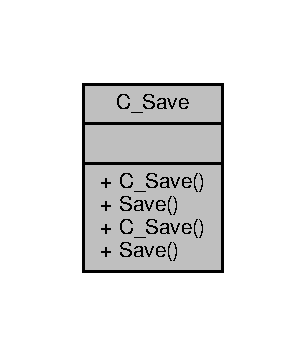
\includegraphics[width=147pt]{classC__Save__coll__graph}
\end{center}
\end{figure}
\subsection*{Public Member Functions}
\begin{DoxyCompactItemize}
\item 
\hyperlink{classC__Save_adc49f753d7b0f40c95ec2b93f81b9672}{C\+\_\+\+Save} ()
\item 
bool \hyperlink{classC__Save_a144be848679b771afb9cf410710308e8}{Save} (const std\+::vector$<$ std\+::shared\+\_\+ptr$<$ \hyperlink{classA__Shape}{A\+\_\+\+Shape} $>$$>$ \&Game)
\begin{DoxyCompactList}\small\item\em Save the current board as puzzle file in a page which contains less than 12 files. \end{DoxyCompactList}\end{DoxyCompactItemize}


\subsection{Detailed Description}
Class of the main Saver. 

This class manage everything about the save 

\subsection{Constructor \& Destructor Documentation}
\mbox{\Hypertarget{classC__Save_adc49f753d7b0f40c95ec2b93f81b9672}\label{classC__Save_adc49f753d7b0f40c95ec2b93f81b9672}} 
\index{C\+\_\+\+Save@{C\+\_\+\+Save}!C\+\_\+\+Save@{C\+\_\+\+Save}}
\index{C\+\_\+\+Save@{C\+\_\+\+Save}!C\+\_\+\+Save@{C\+\_\+\+Save}}
\subsubsection{\texorpdfstring{C\+\_\+\+Save()}{C\_Save()}}
{\footnotesize\ttfamily C\+\_\+\+Save\+::\+C\+\_\+\+Save (\begin{DoxyParamCaption}{ }\end{DoxyParamCaption})}

Construct an instance of a saver 

\subsection{Member Function Documentation}
\mbox{\Hypertarget{classC__Save_a144be848679b771afb9cf410710308e8}\label{classC__Save_a144be848679b771afb9cf410710308e8}} 
\index{C\+\_\+\+Save@{C\+\_\+\+Save}!Save@{Save}}
\index{Save@{Save}!C\+\_\+\+Save@{C\+\_\+\+Save}}
\subsubsection{\texorpdfstring{Save()}{Save()}}
{\footnotesize\ttfamily bool C\+\_\+\+Save\+::\+Save (\begin{DoxyParamCaption}\item[{const std\+::vector$<$ std\+::shared\+\_\+ptr$<$ \hyperlink{classA__Shape}{A\+\_\+\+Shape} $>$$>$ \&}]{Game }\end{DoxyParamCaption})}



Save the current board as puzzle file in a page which contains less than 12 files. 


\begin{DoxyParams}{Parameters}
{\em Game} & \+: Current game \\
\hline
\end{DoxyParams}
\begin{DoxyReturn}{Returns}
Return true if the board has been saved, false otherwise 
\end{DoxyReturn}


The documentation for this class was generated from the following files\+:\begin{DoxyCompactItemize}
\item 
include/parser/\hyperlink{C__Save_8hpp}{C\+\_\+\+Save.\+hpp}\item 
src/parser/\hyperlink{C__Save_8cpp}{C\+\_\+\+Save.\+cpp}\end{DoxyCompactItemize}

\hypertarget{classC__Square}{}\section{C\+\_\+\+Square Class Reference}
\label{classC__Square}\index{C\+\_\+\+Square@{C\+\_\+\+Square}}


Class of the square.  




{\ttfamily \#include $<$C\+\_\+\+Square.\+hpp$>$}



Inheritance diagram for C\+\_\+\+Square\+:
\nopagebreak
\begin{figure}[H]
\begin{center}
\leavevmode
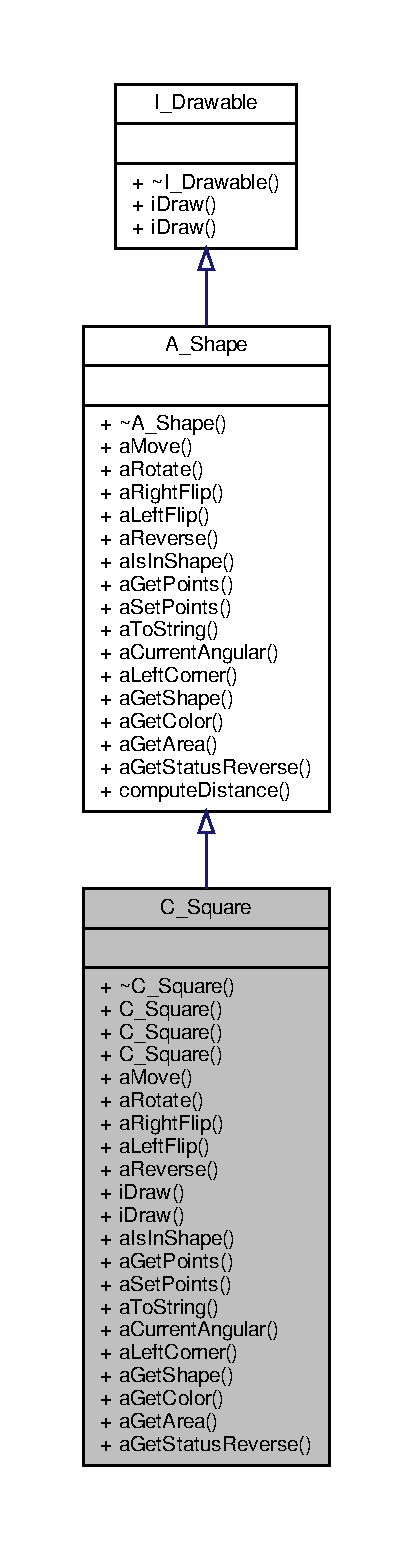
\includegraphics[height=550pt]{classC__Square__inherit__graph}
\end{center}
\end{figure}


Collaboration diagram for C\+\_\+\+Square\+:
\nopagebreak
\begin{figure}[H]
\begin{center}
\leavevmode
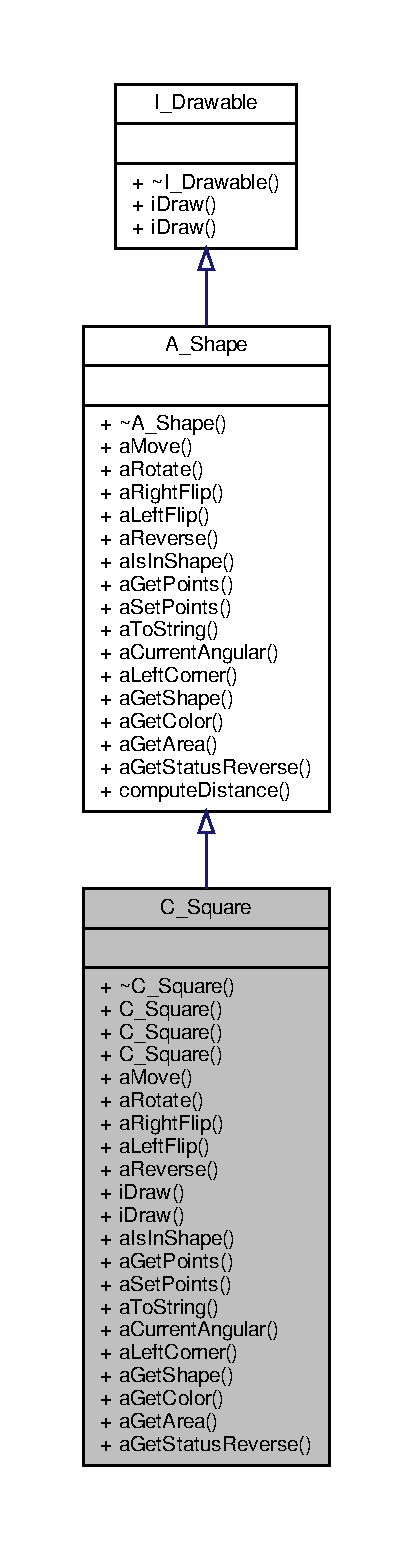
\includegraphics[height=550pt]{classC__Square__coll__graph}
\end{center}
\end{figure}
\subsection*{Public Member Functions}
\begin{DoxyCompactItemize}
\item 
\hyperlink{classC__Square_a8b63c0c06cdda3835b85c4a38692ac44}{$\sim$\+C\+\_\+\+Square} () override
\begin{DoxyCompactList}\small\item\em Destructor of \hyperlink{classC__Square}{C\+\_\+\+Square}. \end{DoxyCompactList}\item 
\hyperlink{classC__Square_a3bec8a18c9b487b44585a38161cb6442}{C\+\_\+\+Square} (M\+L\+V\+\_\+\+Color color=M\+L\+V\+\_\+\+C\+O\+L\+O\+R\+\_\+\+P\+U\+R\+P\+LE)
\begin{DoxyCompactList}\small\item\em Constructor by default of \hyperlink{classC__Square}{C\+\_\+\+Square}, make a \hyperlink{classC__Square}{C\+\_\+\+Square} as default. \end{DoxyCompactList}\item 
\hyperlink{classC__Square_a6e100fed46e6b54971674c60a5f1d87b}{C\+\_\+\+Square} (const std\+::vector$<$ \hyperlink{classC__STriangle}{C\+\_\+\+S\+Triangle} $>$ \&triangle, M\+L\+V\+\_\+\+Color color=M\+L\+V\+\_\+\+C\+O\+L\+O\+R\+\_\+\+P\+U\+R\+P\+LE)
\begin{DoxyCompactList}\small\item\em Constructor of \hyperlink{classC__Square}{C\+\_\+\+Square}, requires a vector of S\+Triangles. \end{DoxyCompactList}\item 
\hyperlink{classC__Square_ac1c9c3504fff971ec8cdbec9f97b020b}{C\+\_\+\+Square} (const \hyperlink{classT__Point}{T\+\_\+\+Point}$<$ double $>$ \&origin, double angular=0.\+0, M\+L\+V\+\_\+\+Color color=M\+L\+V\+\_\+\+C\+O\+L\+O\+R\+\_\+\+P\+U\+R\+P\+LE)
\begin{DoxyCompactList}\small\item\em Constructor of \hyperlink{classC__Square}{C\+\_\+\+Square}, calls the deleguate Default Constructor. \end{DoxyCompactList}\item 
void \hyperlink{classC__Square_a6727523558c58dcd240ec080f254e7c9}{a\+Move} (const \hyperlink{classT__Point}{T\+\_\+\+Point}$<$ double $>$ \&translation) override
\begin{DoxyCompactList}\small\item\em Move the \hyperlink{classC__Square}{C\+\_\+\+Square} by point translation. \end{DoxyCompactList}\item 
void \hyperlink{classC__Square_af74175a5e8d61216d68fde18ef9c9481}{a\+Rotate} (double angular) override
\begin{DoxyCompactList}\small\item\em Rotate the \hyperlink{classC__Square}{C\+\_\+\+Square} with specified angular. \end{DoxyCompactList}\item 
void \hyperlink{classC__Square_a0ea2df0d283ee4ffa911163e55a0a637}{a\+Right\+Flip} () override
\begin{DoxyCompactList}\small\item\em Flip the figure as 45° clock. \end{DoxyCompactList}\item 
void \hyperlink{classC__Square_a31d31862502f0ed24e8331af30100338}{a\+Left\+Flip} () override
\begin{DoxyCompactList}\small\item\em Flip the figure as 45° anti clock. \end{DoxyCompactList}\item 
void \hyperlink{classC__Square_a961d1f5c49a45459668744d459863bd2}{a\+Reverse} () override
\begin{DoxyCompactList}\small\item\em Reverse the figure as symmetry. \end{DoxyCompactList}\item 
void \hyperlink{classC__Square_ae6c51a7720576bcbb94b52584552df28}{i\+Draw} () override
\begin{DoxyCompactList}\small\item\em Draw this shape on I\+HM. \end{DoxyCompactList}\item 
void \hyperlink{classC__Square_a47a80c25bbeda17f17a8230127b4a5ed}{i\+Draw} (M\+L\+V\+\_\+\+Color color) override
\begin{DoxyCompactList}\small\item\em Draw this shape on I\+HM with specific color. \end{DoxyCompactList}\item 
bool \hyperlink{classC__Square_ac5ffad4afca051f117b43012fb4dc239}{a\+Is\+In\+Shape} (const \hyperlink{classT__Point}{T\+\_\+\+Point}$<$ double $>$ \&click) override
\begin{DoxyCompactList}\small\item\em Check if a point is in this shape. \end{DoxyCompactList}\item 
std\+::vector$<$ \hyperlink{classT__Point}{T\+\_\+\+Point}$<$ double $>$ $>$ \hyperlink{classC__Square_aca738fec39149ed697f3d2413cd7cec2}{a\+Get\+Points} () override
\begin{DoxyCompactList}\small\item\em Get m\+Points of this shape. \end{DoxyCompactList}\item 
bool \hyperlink{classC__Square_a295a170686422b745587a250ebe08a5e}{a\+Set\+Points} (const \hyperlink{classT__Point}{T\+\_\+\+Point}$<$ double $>$ \&ref, const \hyperlink{classT__Point}{T\+\_\+\+Point}$<$ double $>$ \&changed) override
\begin{DoxyCompactList}\small\item\em Set a point to another one. \end{DoxyCompactList}\item 
std\+::string \hyperlink{classC__Square_ab2cada51b25cd35b9a79e461767e56f0}{a\+To\+String} () override
\begin{DoxyCompactList}\small\item\em Convert all data of \hyperlink{classC__Square}{C\+\_\+\+Square} in a string. \end{DoxyCompactList}\item 
double \hyperlink{classC__Square_ac7779503b305fda4147b735622c66f81}{a\+Current\+Angular} () override
\begin{DoxyCompactList}\small\item\em Get the current angular of this shape. \end{DoxyCompactList}\item 
\hyperlink{classT__Point}{T\+\_\+\+Point}$<$ double $>$ \hyperlink{classC__Square_a13e97bb379f1678636e3baf781c2a01b}{a\+Left\+Corner} () override
\begin{DoxyCompactList}\small\item\em Take the point at left top corner. \end{DoxyCompactList}\item 
std\+::string \hyperlink{classC__Square_a4919017d3750c1b8deb5f07d22069636}{a\+Get\+Shape} () override
\begin{DoxyCompactList}\small\item\em Get the shape type. \end{DoxyCompactList}\item 
M\+L\+V\+\_\+\+Color \hyperlink{classC__Square_a44b1e58b20cc98edc774a73742fec9a7}{a\+Get\+Color} () override
\begin{DoxyCompactList}\small\item\em Get the color of the shape. \end{DoxyCompactList}\item 
double \hyperlink{classC__Square_affd2be59872618d5d1955be360fb73e6}{a\+Get\+Area} () override
\begin{DoxyCompactList}\small\item\em Get the area of the shape. \end{DoxyCompactList}\item 
bool \hyperlink{classC__Square_afe17127df3b112178973ad2182fe9204}{a\+Get\+Status\+Reverse} () const override
\begin{DoxyCompactList}\small\item\em Get the status of shape reversed or not. \end{DoxyCompactList}\end{DoxyCompactItemize}
\subsection*{Additional Inherited Members}


\subsection{Detailed Description}
Class of the square. 

This class manage everything about the \hyperlink{classC__Square}{C\+\_\+\+Square} 

\subsection{Constructor \& Destructor Documentation}
\mbox{\Hypertarget{classC__Square_a8b63c0c06cdda3835b85c4a38692ac44}\label{classC__Square_a8b63c0c06cdda3835b85c4a38692ac44}} 
\index{C\+\_\+\+Square@{C\+\_\+\+Square}!````~C\+\_\+\+Square@{$\sim$\+C\+\_\+\+Square}}
\index{````~C\+\_\+\+Square@{$\sim$\+C\+\_\+\+Square}!C\+\_\+\+Square@{C\+\_\+\+Square}}
\subsubsection{\texorpdfstring{$\sim$\+C\+\_\+\+Square()}{~C\_Square()}}
{\footnotesize\ttfamily C\+\_\+\+Square\+::$\sim$\+C\+\_\+\+Square (\begin{DoxyParamCaption}{ }\end{DoxyParamCaption})\hspace{0.3cm}{\ttfamily [override]}}



Destructor of \hyperlink{classC__Square}{C\+\_\+\+Square}. 

\mbox{\Hypertarget{classC__Square_a3bec8a18c9b487b44585a38161cb6442}\label{classC__Square_a3bec8a18c9b487b44585a38161cb6442}} 
\index{C\+\_\+\+Square@{C\+\_\+\+Square}!C\+\_\+\+Square@{C\+\_\+\+Square}}
\index{C\+\_\+\+Square@{C\+\_\+\+Square}!C\+\_\+\+Square@{C\+\_\+\+Square}}
\subsubsection{\texorpdfstring{C\+\_\+\+Square()}{C\_Square()}\hspace{0.1cm}{\footnotesize\ttfamily [1/3]}}
{\footnotesize\ttfamily C\+\_\+\+Square\+::\+C\+\_\+\+Square (\begin{DoxyParamCaption}\item[{M\+L\+V\+\_\+\+Color}]{color = {\ttfamily MLV\+\_\+COLOR\+\_\+PURPLE} }\end{DoxyParamCaption})\hspace{0.3cm}{\ttfamily [explicit]}}



Constructor by default of \hyperlink{classC__Square}{C\+\_\+\+Square}, make a \hyperlink{classC__Square}{C\+\_\+\+Square} as default. 


\begin{DoxyParams}{Parameters}
{\em color} & \+: Optional \+\_\+\+\_\+\+Parameter, m\+Color of this shape \\
\hline
\end{DoxyParams}
\mbox{\Hypertarget{classC__Square_a6e100fed46e6b54971674c60a5f1d87b}\label{classC__Square_a6e100fed46e6b54971674c60a5f1d87b}} 
\index{C\+\_\+\+Square@{C\+\_\+\+Square}!C\+\_\+\+Square@{C\+\_\+\+Square}}
\index{C\+\_\+\+Square@{C\+\_\+\+Square}!C\+\_\+\+Square@{C\+\_\+\+Square}}
\subsubsection{\texorpdfstring{C\+\_\+\+Square()}{C\_Square()}\hspace{0.1cm}{\footnotesize\ttfamily [2/3]}}
{\footnotesize\ttfamily C\+\_\+\+Square\+::\+C\+\_\+\+Square (\begin{DoxyParamCaption}\item[{const std\+::vector$<$ \hyperlink{classC__STriangle}{C\+\_\+\+S\+Triangle} $>$ \&}]{triangle,  }\item[{M\+L\+V\+\_\+\+Color}]{color = {\ttfamily MLV\+\_\+COLOR\+\_\+PURPLE} }\end{DoxyParamCaption})\hspace{0.3cm}{\ttfamily [explicit]}}



Constructor of \hyperlink{classC__Square}{C\+\_\+\+Square}, requires a vector of S\+Triangles. 


\begin{DoxyParams}{Parameters}
{\em triangle} & \+: The \hyperlink{classC__Square}{C\+\_\+\+Square} will created with a vector of \hyperlink{classC__STriangle}{C\+\_\+\+S\+Triangle} (4) \\
\hline
{\em color} & \+: Optional \+\_\+\+\_\+\+Parameter, m\+Color of this shape \\
\hline
\end{DoxyParams}
\mbox{\Hypertarget{classC__Square_ac1c9c3504fff971ec8cdbec9f97b020b}\label{classC__Square_ac1c9c3504fff971ec8cdbec9f97b020b}} 
\index{C\+\_\+\+Square@{C\+\_\+\+Square}!C\+\_\+\+Square@{C\+\_\+\+Square}}
\index{C\+\_\+\+Square@{C\+\_\+\+Square}!C\+\_\+\+Square@{C\+\_\+\+Square}}
\subsubsection{\texorpdfstring{C\+\_\+\+Square()}{C\_Square()}\hspace{0.1cm}{\footnotesize\ttfamily [3/3]}}
{\footnotesize\ttfamily C\+\_\+\+Square\+::\+C\+\_\+\+Square (\begin{DoxyParamCaption}\item[{const \hyperlink{classT__Point}{T\+\_\+\+Point}$<$ double $>$ \&}]{origin,  }\item[{double}]{angular = {\ttfamily 0.0},  }\item[{M\+L\+V\+\_\+\+Color}]{color = {\ttfamily MLV\+\_\+COLOR\+\_\+PURPLE} }\end{DoxyParamCaption})\hspace{0.3cm}{\ttfamily [explicit]}}



Constructor of \hyperlink{classC__Square}{C\+\_\+\+Square}, calls the deleguate Default Constructor. 


\begin{DoxyParams}{Parameters}
{\em origin} & \+: shifts the figure of a translation of the origin \\
\hline
{\em angular} & \+: Optional \+\_\+\+\_\+\+Parameter (angular=0.\+0 as default), a\+Rotate the figure with an angular \\
\hline
{\em color} & \+: Optional \+\_\+\+\_\+\+Parameter, m\+Color of this shape \\
\hline
\end{DoxyParams}


\subsection{Member Function Documentation}
\mbox{\Hypertarget{classC__Square_ac7779503b305fda4147b735622c66f81}\label{classC__Square_ac7779503b305fda4147b735622c66f81}} 
\index{C\+\_\+\+Square@{C\+\_\+\+Square}!a\+Current\+Angular@{a\+Current\+Angular}}
\index{a\+Current\+Angular@{a\+Current\+Angular}!C\+\_\+\+Square@{C\+\_\+\+Square}}
\subsubsection{\texorpdfstring{a\+Current\+Angular()}{aCurrentAngular()}}
{\footnotesize\ttfamily double C\+\_\+\+Square\+::a\+Current\+Angular (\begin{DoxyParamCaption}{ }\end{DoxyParamCaption})\hspace{0.3cm}{\ttfamily [override]}, {\ttfamily [virtual]}}



Get the current angular of this shape. 

\begin{DoxyReturn}{Returns}

\end{DoxyReturn}


Implements \hyperlink{classA__Shape_a80fa4e009c875dd0ba7fc5bfeeb43f98}{A\+\_\+\+Shape}.

\mbox{\Hypertarget{classC__Square_affd2be59872618d5d1955be360fb73e6}\label{classC__Square_affd2be59872618d5d1955be360fb73e6}} 
\index{C\+\_\+\+Square@{C\+\_\+\+Square}!a\+Get\+Area@{a\+Get\+Area}}
\index{a\+Get\+Area@{a\+Get\+Area}!C\+\_\+\+Square@{C\+\_\+\+Square}}
\subsubsection{\texorpdfstring{a\+Get\+Area()}{aGetArea()}}
{\footnotesize\ttfamily double C\+\_\+\+Square\+::a\+Get\+Area (\begin{DoxyParamCaption}{ }\end{DoxyParamCaption})\hspace{0.3cm}{\ttfamily [override]}, {\ttfamily [virtual]}}



Get the area of the shape. 

\begin{DoxyReturn}{Returns}
Return the area of the shape 
\end{DoxyReturn}


Implements \hyperlink{classA__Shape_a1b142ee2d873d6c217f65de1632e7b6e}{A\+\_\+\+Shape}.

\mbox{\Hypertarget{classC__Square_a44b1e58b20cc98edc774a73742fec9a7}\label{classC__Square_a44b1e58b20cc98edc774a73742fec9a7}} 
\index{C\+\_\+\+Square@{C\+\_\+\+Square}!a\+Get\+Color@{a\+Get\+Color}}
\index{a\+Get\+Color@{a\+Get\+Color}!C\+\_\+\+Square@{C\+\_\+\+Square}}
\subsubsection{\texorpdfstring{a\+Get\+Color()}{aGetColor()}}
{\footnotesize\ttfamily M\+L\+V\+\_\+\+Color C\+\_\+\+Square\+::a\+Get\+Color (\begin{DoxyParamCaption}{ }\end{DoxyParamCaption})\hspace{0.3cm}{\ttfamily [override]}, {\ttfamily [virtual]}}



Get the color of the shape. 

\begin{DoxyReturn}{Returns}
Return the M\+L\+V\+\_\+\+Color of the shape 
\end{DoxyReturn}


Implements \hyperlink{classA__Shape_a1e90c8132d33e4ac84d42f72606193b2}{A\+\_\+\+Shape}.

\mbox{\Hypertarget{classC__Square_aca738fec39149ed697f3d2413cd7cec2}\label{classC__Square_aca738fec39149ed697f3d2413cd7cec2}} 
\index{C\+\_\+\+Square@{C\+\_\+\+Square}!a\+Get\+Points@{a\+Get\+Points}}
\index{a\+Get\+Points@{a\+Get\+Points}!C\+\_\+\+Square@{C\+\_\+\+Square}}
\subsubsection{\texorpdfstring{a\+Get\+Points()}{aGetPoints()}}
{\footnotesize\ttfamily std\+::vector$<$ \hyperlink{classT__Point}{T\+\_\+\+Point}$<$ double $>$ $>$ C\+\_\+\+Square\+::a\+Get\+Points (\begin{DoxyParamCaption}{ }\end{DoxyParamCaption})\hspace{0.3cm}{\ttfamily [override]}, {\ttfamily [virtual]}}



Get m\+Points of this shape. 

\begin{DoxyReturn}{Returns}
Return a vector of m\+Points of this shape 
\end{DoxyReturn}


Implements \hyperlink{classA__Shape_a9fd1285bd63b1fc88943c9969bf01a5c}{A\+\_\+\+Shape}.

\mbox{\Hypertarget{classC__Square_a4919017d3750c1b8deb5f07d22069636}\label{classC__Square_a4919017d3750c1b8deb5f07d22069636}} 
\index{C\+\_\+\+Square@{C\+\_\+\+Square}!a\+Get\+Shape@{a\+Get\+Shape}}
\index{a\+Get\+Shape@{a\+Get\+Shape}!C\+\_\+\+Square@{C\+\_\+\+Square}}
\subsubsection{\texorpdfstring{a\+Get\+Shape()}{aGetShape()}}
{\footnotesize\ttfamily std\+::string C\+\_\+\+Square\+::a\+Get\+Shape (\begin{DoxyParamCaption}{ }\end{DoxyParamCaption})\hspace{0.3cm}{\ttfamily [override]}, {\ttfamily [virtual]}}



Get the shape type. 

\begin{DoxyReturn}{Returns}
Return as string the shape type 
\end{DoxyReturn}


Implements \hyperlink{classA__Shape_a1b202256a4e5dcb0edab4ab93a37122c}{A\+\_\+\+Shape}.

\mbox{\Hypertarget{classC__Square_afe17127df3b112178973ad2182fe9204}\label{classC__Square_afe17127df3b112178973ad2182fe9204}} 
\index{C\+\_\+\+Square@{C\+\_\+\+Square}!a\+Get\+Status\+Reverse@{a\+Get\+Status\+Reverse}}
\index{a\+Get\+Status\+Reverse@{a\+Get\+Status\+Reverse}!C\+\_\+\+Square@{C\+\_\+\+Square}}
\subsubsection{\texorpdfstring{a\+Get\+Status\+Reverse()}{aGetStatusReverse()}}
{\footnotesize\ttfamily bool C\+\_\+\+Square\+::a\+Get\+Status\+Reverse (\begin{DoxyParamCaption}{ }\end{DoxyParamCaption}) const\hspace{0.3cm}{\ttfamily [override]}, {\ttfamily [virtual]}}



Get the status of shape reversed or not. 

\begin{DoxyReturn}{Returns}
Return true if the shape got reversed, false otherwise 
\end{DoxyReturn}


Implements \hyperlink{classA__Shape_a24991f7667367b646cae75f60df22e28}{A\+\_\+\+Shape}.

\mbox{\Hypertarget{classC__Square_ac5ffad4afca051f117b43012fb4dc239}\label{classC__Square_ac5ffad4afca051f117b43012fb4dc239}} 
\index{C\+\_\+\+Square@{C\+\_\+\+Square}!a\+Is\+In\+Shape@{a\+Is\+In\+Shape}}
\index{a\+Is\+In\+Shape@{a\+Is\+In\+Shape}!C\+\_\+\+Square@{C\+\_\+\+Square}}
\subsubsection{\texorpdfstring{a\+Is\+In\+Shape()}{aIsInShape()}}
{\footnotesize\ttfamily bool C\+\_\+\+Square\+::a\+Is\+In\+Shape (\begin{DoxyParamCaption}\item[{const \hyperlink{classT__Point}{T\+\_\+\+Point}$<$ double $>$ \&}]{click }\end{DoxyParamCaption})\hspace{0.3cm}{\ttfamily [override]}, {\ttfamily [virtual]}}



Check if a point is in this shape. 


\begin{DoxyParams}{Parameters}
{\em click} & \+: \hyperlink{classT__Point}{T\+\_\+\+Point} to check \\
\hline
\end{DoxyParams}
\begin{DoxyReturn}{Returns}
true if Click is in this shape, false if not 
\end{DoxyReturn}


Implements \hyperlink{classA__Shape_a63f825cbc9780208d9a137f5c14917d0}{A\+\_\+\+Shape}.

\mbox{\Hypertarget{classC__Square_a13e97bb379f1678636e3baf781c2a01b}\label{classC__Square_a13e97bb379f1678636e3baf781c2a01b}} 
\index{C\+\_\+\+Square@{C\+\_\+\+Square}!a\+Left\+Corner@{a\+Left\+Corner}}
\index{a\+Left\+Corner@{a\+Left\+Corner}!C\+\_\+\+Square@{C\+\_\+\+Square}}
\subsubsection{\texorpdfstring{a\+Left\+Corner()}{aLeftCorner()}}
{\footnotesize\ttfamily \hyperlink{classT__Point}{T\+\_\+\+Point}$<$ double $>$ C\+\_\+\+Square\+::a\+Left\+Corner (\begin{DoxyParamCaption}{ }\end{DoxyParamCaption})\hspace{0.3cm}{\ttfamily [override]}, {\ttfamily [virtual]}}



Take the point at left top corner. 

\begin{DoxyReturn}{Returns}
Return the point at left top corner 
\end{DoxyReturn}


Implements \hyperlink{classA__Shape_abe6781b13037bf7ecea8ff9456b31533}{A\+\_\+\+Shape}.

\mbox{\Hypertarget{classC__Square_a31d31862502f0ed24e8331af30100338}\label{classC__Square_a31d31862502f0ed24e8331af30100338}} 
\index{C\+\_\+\+Square@{C\+\_\+\+Square}!a\+Left\+Flip@{a\+Left\+Flip}}
\index{a\+Left\+Flip@{a\+Left\+Flip}!C\+\_\+\+Square@{C\+\_\+\+Square}}
\subsubsection{\texorpdfstring{a\+Left\+Flip()}{aLeftFlip()}}
{\footnotesize\ttfamily void C\+\_\+\+Square\+::a\+Left\+Flip (\begin{DoxyParamCaption}{ }\end{DoxyParamCaption})\hspace{0.3cm}{\ttfamily [override]}, {\ttfamily [virtual]}}



Flip the figure as 45° anti clock. 



Implements \hyperlink{classA__Shape_abe947e7003cb63be2b4f6c439533427d}{A\+\_\+\+Shape}.

\mbox{\Hypertarget{classC__Square_a6727523558c58dcd240ec080f254e7c9}\label{classC__Square_a6727523558c58dcd240ec080f254e7c9}} 
\index{C\+\_\+\+Square@{C\+\_\+\+Square}!a\+Move@{a\+Move}}
\index{a\+Move@{a\+Move}!C\+\_\+\+Square@{C\+\_\+\+Square}}
\subsubsection{\texorpdfstring{a\+Move()}{aMove()}}
{\footnotesize\ttfamily void C\+\_\+\+Square\+::a\+Move (\begin{DoxyParamCaption}\item[{const \hyperlink{classT__Point}{T\+\_\+\+Point}$<$ double $>$ \&}]{translation }\end{DoxyParamCaption})\hspace{0.3cm}{\ttfamily [override]}, {\ttfamily [virtual]}}



Move the \hyperlink{classC__Square}{C\+\_\+\+Square} by point translation. 


\begin{DoxyParams}{Parameters}
{\em translation} & \+: Every m\+Points of this shape will be translate by this \+\_\+\+\_\+\+Parameter \\
\hline
\end{DoxyParams}


Implements \hyperlink{classA__Shape_ab284298db1b557ccfa7ba6de7a5fee2c}{A\+\_\+\+Shape}.

\mbox{\Hypertarget{classC__Square_a961d1f5c49a45459668744d459863bd2}\label{classC__Square_a961d1f5c49a45459668744d459863bd2}} 
\index{C\+\_\+\+Square@{C\+\_\+\+Square}!a\+Reverse@{a\+Reverse}}
\index{a\+Reverse@{a\+Reverse}!C\+\_\+\+Square@{C\+\_\+\+Square}}
\subsubsection{\texorpdfstring{a\+Reverse()}{aReverse()}}
{\footnotesize\ttfamily void C\+\_\+\+Square\+::a\+Reverse (\begin{DoxyParamCaption}{ }\end{DoxyParamCaption})\hspace{0.3cm}{\ttfamily [override]}, {\ttfamily [virtual]}}



Reverse the figure as symmetry. 



Implements \hyperlink{classA__Shape_afe2c7969d647f6358da13879a7534ecb}{A\+\_\+\+Shape}.

\mbox{\Hypertarget{classC__Square_a0ea2df0d283ee4ffa911163e55a0a637}\label{classC__Square_a0ea2df0d283ee4ffa911163e55a0a637}} 
\index{C\+\_\+\+Square@{C\+\_\+\+Square}!a\+Right\+Flip@{a\+Right\+Flip}}
\index{a\+Right\+Flip@{a\+Right\+Flip}!C\+\_\+\+Square@{C\+\_\+\+Square}}
\subsubsection{\texorpdfstring{a\+Right\+Flip()}{aRightFlip()}}
{\footnotesize\ttfamily void C\+\_\+\+Square\+::a\+Right\+Flip (\begin{DoxyParamCaption}{ }\end{DoxyParamCaption})\hspace{0.3cm}{\ttfamily [override]}, {\ttfamily [virtual]}}



Flip the figure as 45° clock. 



Implements \hyperlink{classA__Shape_a892688cbbad3297e00e87cce0dbfc76d}{A\+\_\+\+Shape}.

\mbox{\Hypertarget{classC__Square_af74175a5e8d61216d68fde18ef9c9481}\label{classC__Square_af74175a5e8d61216d68fde18ef9c9481}} 
\index{C\+\_\+\+Square@{C\+\_\+\+Square}!a\+Rotate@{a\+Rotate}}
\index{a\+Rotate@{a\+Rotate}!C\+\_\+\+Square@{C\+\_\+\+Square}}
\subsubsection{\texorpdfstring{a\+Rotate()}{aRotate()}}
{\footnotesize\ttfamily void C\+\_\+\+Square\+::a\+Rotate (\begin{DoxyParamCaption}\item[{double}]{angular }\end{DoxyParamCaption})\hspace{0.3cm}{\ttfamily [override]}, {\ttfamily [virtual]}}



Rotate the \hyperlink{classC__Square}{C\+\_\+\+Square} with specified angular. 


\begin{DoxyParams}{Parameters}
{\em angular} & \+: This angular should be between (0, 2\+PI) \\
\hline
\end{DoxyParams}


Implements \hyperlink{classA__Shape_a25b4e0c34cdb46da5382fe9c7467efaf}{A\+\_\+\+Shape}.

\mbox{\Hypertarget{classC__Square_a295a170686422b745587a250ebe08a5e}\label{classC__Square_a295a170686422b745587a250ebe08a5e}} 
\index{C\+\_\+\+Square@{C\+\_\+\+Square}!a\+Set\+Points@{a\+Set\+Points}}
\index{a\+Set\+Points@{a\+Set\+Points}!C\+\_\+\+Square@{C\+\_\+\+Square}}
\subsubsection{\texorpdfstring{a\+Set\+Points()}{aSetPoints()}}
{\footnotesize\ttfamily bool C\+\_\+\+Square\+::a\+Set\+Points (\begin{DoxyParamCaption}\item[{const \hyperlink{classT__Point}{T\+\_\+\+Point}$<$ double $>$ \&}]{ref,  }\item[{const \hyperlink{classT__Point}{T\+\_\+\+Point}$<$ double $>$ \&}]{changed }\end{DoxyParamCaption})\hspace{0.3cm}{\ttfamily [override]}, {\ttfamily [virtual]}}



Set a point to another one. 


\begin{DoxyParams}{Parameters}
{\em ref} & \+: Point to change \\
\hline
{\em changed} & \+: New value of the point \\
\hline
\end{DoxyParams}
\begin{DoxyReturn}{Returns}
True if the ref point exists, false otherwise 
\end{DoxyReturn}


Implements \hyperlink{classA__Shape_a6996f454b337f8425ad13cba3f7a7c35}{A\+\_\+\+Shape}.

\mbox{\Hypertarget{classC__Square_ab2cada51b25cd35b9a79e461767e56f0}\label{classC__Square_ab2cada51b25cd35b9a79e461767e56f0}} 
\index{C\+\_\+\+Square@{C\+\_\+\+Square}!a\+To\+String@{a\+To\+String}}
\index{a\+To\+String@{a\+To\+String}!C\+\_\+\+Square@{C\+\_\+\+Square}}
\subsubsection{\texorpdfstring{a\+To\+String()}{aToString()}}
{\footnotesize\ttfamily std\+::string C\+\_\+\+Square\+::a\+To\+String (\begin{DoxyParamCaption}{ }\end{DoxyParamCaption})\hspace{0.3cm}{\ttfamily [override]}, {\ttfamily [virtual]}}



Convert all data of \hyperlink{classC__Square}{C\+\_\+\+Square} in a string. 

\begin{DoxyReturn}{Returns}
Return a string which contains every m\+Points of this shape 
\end{DoxyReturn}


Implements \hyperlink{classA__Shape_ad8804b4e74543db374af6892367b7c2e}{A\+\_\+\+Shape}.

\mbox{\Hypertarget{classC__Square_ae6c51a7720576bcbb94b52584552df28}\label{classC__Square_ae6c51a7720576bcbb94b52584552df28}} 
\index{C\+\_\+\+Square@{C\+\_\+\+Square}!i\+Draw@{i\+Draw}}
\index{i\+Draw@{i\+Draw}!C\+\_\+\+Square@{C\+\_\+\+Square}}
\subsubsection{\texorpdfstring{i\+Draw()}{iDraw()}\hspace{0.1cm}{\footnotesize\ttfamily [1/2]}}
{\footnotesize\ttfamily void C\+\_\+\+Square\+::i\+Draw (\begin{DoxyParamCaption}{ }\end{DoxyParamCaption})\hspace{0.3cm}{\ttfamily [override]}, {\ttfamily [virtual]}}



Draw this shape on I\+HM. 



Implements \hyperlink{classI__Drawable_ae24c65000977a805f52ce032321cd86f}{I\+\_\+\+Drawable}.

\mbox{\Hypertarget{classC__Square_a47a80c25bbeda17f17a8230127b4a5ed}\label{classC__Square_a47a80c25bbeda17f17a8230127b4a5ed}} 
\index{C\+\_\+\+Square@{C\+\_\+\+Square}!i\+Draw@{i\+Draw}}
\index{i\+Draw@{i\+Draw}!C\+\_\+\+Square@{C\+\_\+\+Square}}
\subsubsection{\texorpdfstring{i\+Draw()}{iDraw()}\hspace{0.1cm}{\footnotesize\ttfamily [2/2]}}
{\footnotesize\ttfamily void C\+\_\+\+Square\+::i\+Draw (\begin{DoxyParamCaption}\item[{M\+L\+V\+\_\+\+Color}]{color }\end{DoxyParamCaption})\hspace{0.3cm}{\ttfamily [override]}, {\ttfamily [virtual]}}



Draw this shape on I\+HM with specific color. 


\begin{DoxyParams}{Parameters}
{\em color} & \+: color of the shape will be draw \\
\hline
\end{DoxyParams}


Implements \hyperlink{classI__Drawable_a25f6474325614c451a91f019e5fe8010}{I\+\_\+\+Drawable}.



The documentation for this class was generated from the following files\+:\begin{DoxyCompactItemize}
\item 
include/shape/\hyperlink{C__Square_8hpp}{C\+\_\+\+Square.\+hpp}\item 
src/shape/\hyperlink{C__Square_8cpp}{C\+\_\+\+Square.\+cpp}\end{DoxyCompactItemize}

\hypertarget{classC__STriangle}{}\section{C\+\_\+\+S\+Triangle Class Reference}
\label{classC__STriangle}\index{C\+\_\+\+S\+Triangle@{C\+\_\+\+S\+Triangle}}


Class of the small m\+Triangles.  




{\ttfamily \#include $<$C\+\_\+\+S\+Triangle.\+hpp$>$}



Inheritance diagram for C\+\_\+\+S\+Triangle\+:\nopagebreak
\begin{figure}[H]
\begin{center}
\leavevmode
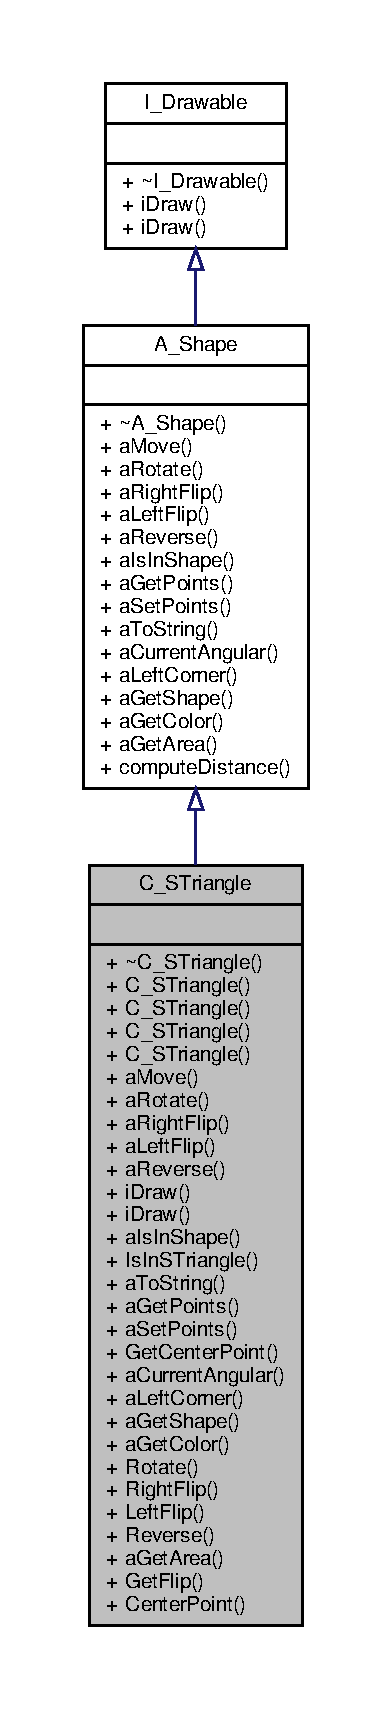
\includegraphics[height=550pt]{classC__STriangle__inherit__graph}
\end{center}
\end{figure}


Collaboration diagram for C\+\_\+\+S\+Triangle\+:\nopagebreak
\begin{figure}[H]
\begin{center}
\leavevmode
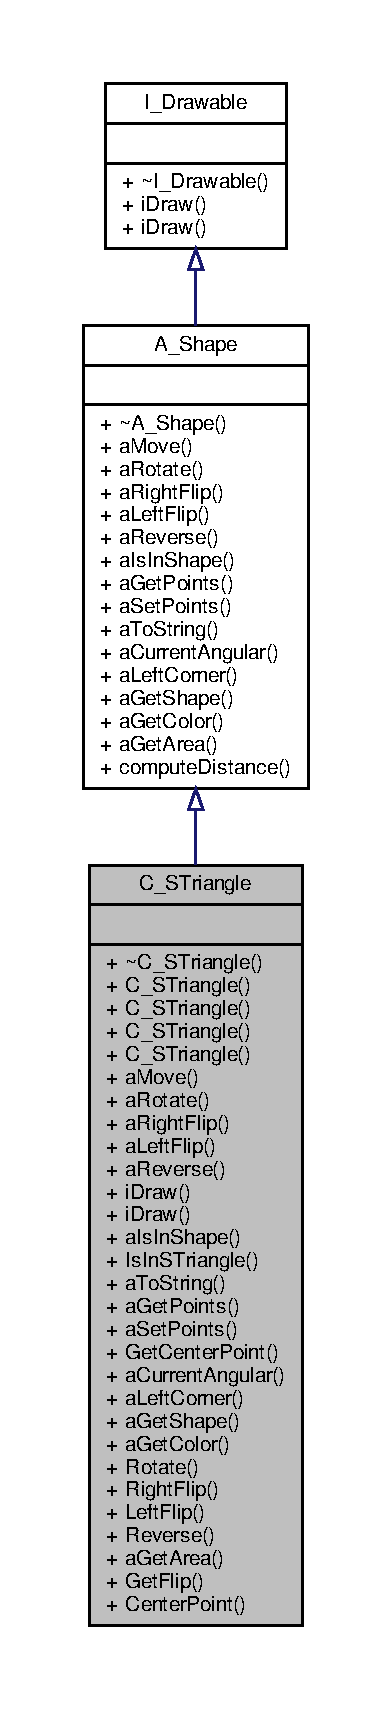
\includegraphics[height=550pt]{classC__STriangle__coll__graph}
\end{center}
\end{figure}
\subsection*{Public Member Functions}
\begin{DoxyCompactItemize}
\item 
\hyperlink{classC__STriangle_a545f9a8f64e89a4b1269f7ea93251e64}{$\sim$\+C\+\_\+\+S\+Triangle} () override
\begin{DoxyCompactList}\small\item\em Destructor of \hyperlink{classC__STriangle}{C\+\_\+\+S\+Triangle}. \end{DoxyCompactList}\item 
\hyperlink{classC__STriangle_a3fcf5957768e63aded3872349d3a0397}{C\+\_\+\+S\+Triangle} (M\+L\+V\+\_\+\+Color color=M\+L\+V\+\_\+\+C\+O\+L\+O\+R\+\_\+\+G\+R\+E\+EN)
\begin{DoxyCompactList}\small\item\em Constructor by default of \hyperlink{classC__MTriangle}{C\+\_\+\+M\+Triangle}, make a \hyperlink{classC__STriangle}{C\+\_\+\+S\+Triangle} as default. \end{DoxyCompactList}\item 
\hyperlink{classC__STriangle_a7d3fe40c752838aab0116af91b3a2b28}{C\+\_\+\+S\+Triangle} (const \hyperlink{classT__Point}{T\+\_\+\+Point}$<$ double $>$ \&p1, const \hyperlink{classT__Point}{T\+\_\+\+Point}$<$ double $>$ \&p2, const \hyperlink{classT__Point}{T\+\_\+\+Point}$<$ double $>$ \&p3, M\+L\+V\+\_\+\+Color color=M\+L\+V\+\_\+\+C\+O\+L\+O\+R\+\_\+\+G\+R\+E\+EN)
\begin{DoxyCompactList}\small\item\em Constructor of \hyperlink{classC__STriangle}{C\+\_\+\+S\+Triangle}, requires 3 m\+Points. \end{DoxyCompactList}\item 
\hyperlink{classC__STriangle_acaabdb10b1689d1b26f655c266d34996}{C\+\_\+\+S\+Triangle} (const std\+::vector$<$ \hyperlink{classT__Point}{T\+\_\+\+Point}$<$ double $>$$>$ \&points, M\+L\+V\+\_\+\+Color color=M\+L\+V\+\_\+\+C\+O\+L\+O\+R\+\_\+\+G\+R\+E\+EN)
\begin{DoxyCompactList}\small\item\em Constructor of \hyperlink{classC__STriangle}{C\+\_\+\+S\+Triangle}, requires a vector of 3 m\+Points. \end{DoxyCompactList}\item 
\hyperlink{classC__STriangle_aee7b2ac8280dde9b86f5c3ad973fd692}{C\+\_\+\+S\+Triangle} (const \hyperlink{classT__Point}{T\+\_\+\+Point}$<$ double $>$ \&origin, double angular=0.\+0, M\+L\+V\+\_\+\+Color color=M\+L\+V\+\_\+\+C\+O\+L\+O\+R\+\_\+\+G\+R\+E\+EN)
\begin{DoxyCompactList}\small\item\em Constructor of \hyperlink{classC__STriangle}{C\+\_\+\+S\+Triangle}, calls the deleguate Default Constructor. \end{DoxyCompactList}\item 
void \hyperlink{classC__STriangle_a82a3c3a847ca6c2d5922921150fa50b5}{a\+Move} (const \hyperlink{classT__Point}{T\+\_\+\+Point}$<$ double $>$ \&translation) override
\begin{DoxyCompactList}\small\item\em Move the \hyperlink{classC__MTriangle}{C\+\_\+\+M\+Triangle} by point translation. \end{DoxyCompactList}\item 
void \hyperlink{classC__STriangle_a52612242aba17043862355c030637a18}{a\+Rotate} (double angular) override
\begin{DoxyCompactList}\small\item\em Rotate the \hyperlink{classC__STriangle}{C\+\_\+\+S\+Triangle} with specified angular. \end{DoxyCompactList}\item 
void \hyperlink{classC__STriangle_aa3cad7b7367c253000cf0f91f55ba600}{a\+Right\+Flip} () override
\begin{DoxyCompactList}\small\item\em Flip the figure as 45° clock. \end{DoxyCompactList}\item 
void \hyperlink{classC__STriangle_aff480b9ec706ee5ae58f6f78318e2728}{a\+Left\+Flip} () override
\begin{DoxyCompactList}\small\item\em Flip the figure as 45° anti clock. \end{DoxyCompactList}\item 
void \hyperlink{classC__STriangle_a5402899ec4ea0de3ca3e7aa6f184a1c7}{a\+Reverse} () override
\begin{DoxyCompactList}\small\item\em Reverse the figure as symmetry. \end{DoxyCompactList}\item 
void \hyperlink{classC__STriangle_a7297480fe52b58654d81e2e70fbb237d}{i\+Draw} () override
\begin{DoxyCompactList}\small\item\em Draw this shape on I\+HM. \end{DoxyCompactList}\item 
void \hyperlink{classC__STriangle_ad003b932a467de60b814d897fda38390}{i\+Draw} (M\+L\+V\+\_\+\+Color color) override
\begin{DoxyCompactList}\small\item\em Draw this shape on I\+HM with specific m\+Color. \end{DoxyCompactList}\item 
bool \hyperlink{classC__STriangle_a3bc82d7ea53a6a058b9fb49bbd89282c}{a\+Is\+In\+Shape} (const \hyperlink{classT__Point}{T\+\_\+\+Point}$<$ double $>$ \&click) override
\begin{DoxyCompactList}\small\item\em Check if a point is in this shape. \end{DoxyCompactList}\item 
bool \hyperlink{classC__STriangle_ae0cfadc631baf280df7e77f011489caa}{Is\+In\+S\+Triangle} (const \hyperlink{classT__Point}{T\+\_\+\+Point}$<$ double $>$ \&click)
\begin{DoxyCompactList}\small\item\em Check if a point is in this \hyperlink{classC__STriangle}{C\+\_\+\+S\+Triangle}. \end{DoxyCompactList}\item 
std\+::string \hyperlink{classC__STriangle_a1ea089f6a82c2770e0529c4a9fc07d90}{a\+To\+String} () override
\begin{DoxyCompactList}\small\item\em Convert all data of \hyperlink{classC__MTriangle}{C\+\_\+\+M\+Triangle} in a string. \end{DoxyCompactList}\item 
std\+::vector$<$ \hyperlink{classT__Point}{T\+\_\+\+Point}$<$ double $>$ $>$ \hyperlink{classC__STriangle_a8d144f4451fe2e5bf6f333d8c37f0f57}{a\+Get\+Points} () override
\begin{DoxyCompactList}\small\item\em Get every m\+Points of this \hyperlink{classC__STriangle}{C\+\_\+\+S\+Triangle}. \end{DoxyCompactList}\item 
bool \hyperlink{classC__STriangle_a431802d5e10b69f535e7929a23963b5e}{a\+Set\+Points} (const \hyperlink{classT__Point}{T\+\_\+\+Point}$<$ double $>$ \&ref, const \hyperlink{classT__Point}{T\+\_\+\+Point}$<$ double $>$ \&changed) override
\begin{DoxyCompactList}\small\item\em Set a point as same value that another point given in parameter. \end{DoxyCompactList}\item 
\hyperlink{classT__Point}{T\+\_\+\+Point}$<$ double $>$ \hyperlink{classC__STriangle_ac9b374f16313b3c99eca7fe615d14851}{Get\+Center\+Point} ()
\begin{DoxyCompactList}\small\item\em Get the current center point of this \hyperlink{classC__STriangle}{C\+\_\+\+S\+Triangle}. \end{DoxyCompactList}\item 
double \hyperlink{classC__STriangle_a38304830925938339c4a4a0ad812e151}{a\+Current\+Angular} () override
\begin{DoxyCompactList}\small\item\em Get the current angular of this shape. \end{DoxyCompactList}\item 
\hyperlink{classT__Point}{T\+\_\+\+Point}$<$ double $>$ \hyperlink{classC__STriangle_a8e580f80693ea6f66cca3782ced8e301}{a\+Left\+Corner} () override
\begin{DoxyCompactList}\small\item\em Take the point at left top corner. \end{DoxyCompactList}\item 
std\+::string \hyperlink{classC__STriangle_a40c1434870b99112c4457819c9295483}{a\+Get\+Shape} () override
\begin{DoxyCompactList}\small\item\em Get the type of shape is it. \end{DoxyCompactList}\item 
M\+L\+V\+\_\+\+Color \hyperlink{classC__STriangle_a1a0c315653ece65118705648d09336dd}{a\+Get\+Color} () override
\begin{DoxyCompactList}\small\item\em Get the color of the shape. \end{DoxyCompactList}\item 
void \hyperlink{classC__STriangle_afe6a1fcb5bf97792dd38e698bb6ad0cd}{Rotate} (double angular, const \hyperlink{classT__Point}{T\+\_\+\+Point}$<$ double $>$ \&center\+\_\+point)
\begin{DoxyCompactList}\small\item\em Rotate an \hyperlink{classC__STriangle}{C\+\_\+\+S\+Triangle} with specified angular, used only for an other shape. \end{DoxyCompactList}\item 
void \hyperlink{classC__STriangle_ad84c7c6c2a4ca6d2fd3a681fd6dfcf63}{Right\+Flip} (const \hyperlink{classT__Point}{T\+\_\+\+Point}$<$ double $>$ \&center\+Point)
\begin{DoxyCompactList}\small\item\em Right flip as 45° clock. \end{DoxyCompactList}\item 
void \hyperlink{classC__STriangle_aec7540d5750509269894dc4c906fc20f}{Left\+Flip} (const \hyperlink{classT__Point}{T\+\_\+\+Point}$<$ double $>$ \&center\+Point)
\begin{DoxyCompactList}\small\item\em Right flip as 45° anti clock. \end{DoxyCompactList}\item 
void \hyperlink{classC__STriangle_a3fafeed75d888024e95a494b8901e8fe}{Reverse} (const \hyperlink{classT__Point}{T\+\_\+\+Point}$<$ double $>$ \&center\+Point)
\begin{DoxyCompactList}\small\item\em Reverse the figure as symmetry. \end{DoxyCompactList}\item 
double \hyperlink{classC__STriangle_aaff25f3c7f7640c3e7c735a77800e96e}{a\+Get\+Area} () override
\begin{DoxyCompactList}\small\item\em Get the area of the shape. \end{DoxyCompactList}\item 
std\+::vector$<$ \hyperlink{classT__Point}{T\+\_\+\+Point}$<$ double $>$ $>$ \hyperlink{classC__STriangle_a92550826ba2d9866f2cb01b66abfbebc}{Get\+Flip} ()
\begin{DoxyCompactList}\small\item\em Get a vector of \char`\"{}flip\char`\"{} needed to flip the figure. \end{DoxyCompactList}\end{DoxyCompactItemize}
\subsection*{Static Public Member Functions}
\begin{DoxyCompactItemize}
\item 
static \hyperlink{classT__Point}{T\+\_\+\+Point}$<$ double $>$ \hyperlink{classC__STriangle_a98c01a7d57aeee85ee4e2df88a786b7f}{Center\+Point} (const std\+::vector$<$ \hyperlink{classT__Point}{T\+\_\+\+Point}$<$ double $>$$>$ \&list\+\_\+points)
\begin{DoxyCompactList}\small\item\em Compute the center point of N m\+Points. \end{DoxyCompactList}\end{DoxyCompactItemize}


\subsection{Detailed Description}
Class of the small m\+Triangles. 

This class manage everything about the small m\+Triangles 

\subsection{Constructor \& Destructor Documentation}
\mbox{\Hypertarget{classC__STriangle_a545f9a8f64e89a4b1269f7ea93251e64}\label{classC__STriangle_a545f9a8f64e89a4b1269f7ea93251e64}} 
\index{C\+\_\+\+S\+Triangle@{C\+\_\+\+S\+Triangle}!````~C\+\_\+\+S\+Triangle@{$\sim$\+C\+\_\+\+S\+Triangle}}
\index{````~C\+\_\+\+S\+Triangle@{$\sim$\+C\+\_\+\+S\+Triangle}!C\+\_\+\+S\+Triangle@{C\+\_\+\+S\+Triangle}}
\subsubsection{\texorpdfstring{$\sim$\+C\+\_\+\+S\+Triangle()}{~C\_STriangle()}}
{\footnotesize\ttfamily C\+\_\+\+S\+Triangle\+::$\sim$\+C\+\_\+\+S\+Triangle (\begin{DoxyParamCaption}{ }\end{DoxyParamCaption})\hspace{0.3cm}{\ttfamily [override]}}



Destructor of \hyperlink{classC__STriangle}{C\+\_\+\+S\+Triangle}. 

\mbox{\Hypertarget{classC__STriangle_a3fcf5957768e63aded3872349d3a0397}\label{classC__STriangle_a3fcf5957768e63aded3872349d3a0397}} 
\index{C\+\_\+\+S\+Triangle@{C\+\_\+\+S\+Triangle}!C\+\_\+\+S\+Triangle@{C\+\_\+\+S\+Triangle}}
\index{C\+\_\+\+S\+Triangle@{C\+\_\+\+S\+Triangle}!C\+\_\+\+S\+Triangle@{C\+\_\+\+S\+Triangle}}
\subsubsection{\texorpdfstring{C\+\_\+\+S\+Triangle()}{C\_STriangle()}\hspace{0.1cm}{\footnotesize\ttfamily [1/4]}}
{\footnotesize\ttfamily C\+\_\+\+S\+Triangle\+::\+C\+\_\+\+S\+Triangle (\begin{DoxyParamCaption}\item[{M\+L\+V\+\_\+\+Color}]{color = {\ttfamily MLV\+\_\+COLOR\+\_\+GREEN} }\end{DoxyParamCaption})\hspace{0.3cm}{\ttfamily [explicit]}}



Constructor by default of \hyperlink{classC__MTriangle}{C\+\_\+\+M\+Triangle}, make a \hyperlink{classC__STriangle}{C\+\_\+\+S\+Triangle} as default. 


\begin{DoxyParams}{Parameters}
{\em color} & \+: Optional \+\_\+\+\_\+\+Parameter, m\+Color of this shape \\
\hline
\end{DoxyParams}
\mbox{\Hypertarget{classC__STriangle_a7d3fe40c752838aab0116af91b3a2b28}\label{classC__STriangle_a7d3fe40c752838aab0116af91b3a2b28}} 
\index{C\+\_\+\+S\+Triangle@{C\+\_\+\+S\+Triangle}!C\+\_\+\+S\+Triangle@{C\+\_\+\+S\+Triangle}}
\index{C\+\_\+\+S\+Triangle@{C\+\_\+\+S\+Triangle}!C\+\_\+\+S\+Triangle@{C\+\_\+\+S\+Triangle}}
\subsubsection{\texorpdfstring{C\+\_\+\+S\+Triangle()}{C\_STriangle()}\hspace{0.1cm}{\footnotesize\ttfamily [2/4]}}
{\footnotesize\ttfamily C\+\_\+\+S\+Triangle\+::\+C\+\_\+\+S\+Triangle (\begin{DoxyParamCaption}\item[{const \hyperlink{classT__Point}{T\+\_\+\+Point}$<$ double $>$ \&}]{p1,  }\item[{const \hyperlink{classT__Point}{T\+\_\+\+Point}$<$ double $>$ \&}]{p2,  }\item[{const \hyperlink{classT__Point}{T\+\_\+\+Point}$<$ double $>$ \&}]{p3,  }\item[{M\+L\+V\+\_\+\+Color}]{color = {\ttfamily MLV\+\_\+COLOR\+\_\+GREEN} }\end{DoxyParamCaption})}



Constructor of \hyperlink{classC__STriangle}{C\+\_\+\+S\+Triangle}, requires 3 m\+Points. 


\begin{DoxyParams}{Parameters}
{\em p1} & \+: First point of the \hyperlink{classC__STriangle}{C\+\_\+\+S\+Triangle} \\
\hline
{\em p2} & \+: Second point of the \hyperlink{classC__STriangle}{C\+\_\+\+S\+Triangle} \\
\hline
{\em p3} & \+: Third point of the \hyperlink{classC__STriangle}{C\+\_\+\+S\+Triangle} \\
\hline
{\em color} & \+: Optional \+\_\+\+\_\+\+Parameter, m\+Color of this shape \\
\hline
\end{DoxyParams}
\mbox{\Hypertarget{classC__STriangle_acaabdb10b1689d1b26f655c266d34996}\label{classC__STriangle_acaabdb10b1689d1b26f655c266d34996}} 
\index{C\+\_\+\+S\+Triangle@{C\+\_\+\+S\+Triangle}!C\+\_\+\+S\+Triangle@{C\+\_\+\+S\+Triangle}}
\index{C\+\_\+\+S\+Triangle@{C\+\_\+\+S\+Triangle}!C\+\_\+\+S\+Triangle@{C\+\_\+\+S\+Triangle}}
\subsubsection{\texorpdfstring{C\+\_\+\+S\+Triangle()}{C\_STriangle()}\hspace{0.1cm}{\footnotesize\ttfamily [3/4]}}
{\footnotesize\ttfamily C\+\_\+\+S\+Triangle\+::\+C\+\_\+\+S\+Triangle (\begin{DoxyParamCaption}\item[{const std\+::vector$<$ \hyperlink{classT__Point}{T\+\_\+\+Point}$<$ double $>$$>$ \&}]{points,  }\item[{M\+L\+V\+\_\+\+Color}]{color = {\ttfamily MLV\+\_\+COLOR\+\_\+GREEN} }\end{DoxyParamCaption})\hspace{0.3cm}{\ttfamily [explicit]}}



Constructor of \hyperlink{classC__STriangle}{C\+\_\+\+S\+Triangle}, requires a vector of 3 m\+Points. 


\begin{DoxyParams}{Parameters}
{\em points} & \+: vector of 3 m\+Points \\
\hline
{\em color} & \+: Optional \+\_\+\+\_\+\+Parameter, m\+Color of this shape \\
\hline
\end{DoxyParams}
\mbox{\Hypertarget{classC__STriangle_aee7b2ac8280dde9b86f5c3ad973fd692}\label{classC__STriangle_aee7b2ac8280dde9b86f5c3ad973fd692}} 
\index{C\+\_\+\+S\+Triangle@{C\+\_\+\+S\+Triangle}!C\+\_\+\+S\+Triangle@{C\+\_\+\+S\+Triangle}}
\index{C\+\_\+\+S\+Triangle@{C\+\_\+\+S\+Triangle}!C\+\_\+\+S\+Triangle@{C\+\_\+\+S\+Triangle}}
\subsubsection{\texorpdfstring{C\+\_\+\+S\+Triangle()}{C\_STriangle()}\hspace{0.1cm}{\footnotesize\ttfamily [4/4]}}
{\footnotesize\ttfamily C\+\_\+\+S\+Triangle\+::\+C\+\_\+\+S\+Triangle (\begin{DoxyParamCaption}\item[{const \hyperlink{classT__Point}{T\+\_\+\+Point}$<$ double $>$ \&}]{origin,  }\item[{double}]{angular = {\ttfamily 0.0},  }\item[{M\+L\+V\+\_\+\+Color}]{color = {\ttfamily MLV\+\_\+COLOR\+\_\+GREEN} }\end{DoxyParamCaption})\hspace{0.3cm}{\ttfamily [explicit]}}



Constructor of \hyperlink{classC__STriangle}{C\+\_\+\+S\+Triangle}, calls the deleguate Default Constructor. 


\begin{DoxyParams}{Parameters}
{\em origin} & \+: shifts the figure of a translation of the origin \\
\hline
{\em angular} & \+: Optional \+\_\+\+\_\+\+Parameter (angular=0.\+0 as default), a\+Rotate the figure with an angular \\
\hline
{\em color} & \+: Optional \+\_\+\+\_\+\+Parameter, m\+Color of this shape \\
\hline
\end{DoxyParams}


\subsection{Member Function Documentation}
\mbox{\Hypertarget{classC__STriangle_a38304830925938339c4a4a0ad812e151}\label{classC__STriangle_a38304830925938339c4a4a0ad812e151}} 
\index{C\+\_\+\+S\+Triangle@{C\+\_\+\+S\+Triangle}!a\+Current\+Angular@{a\+Current\+Angular}}
\index{a\+Current\+Angular@{a\+Current\+Angular}!C\+\_\+\+S\+Triangle@{C\+\_\+\+S\+Triangle}}
\subsubsection{\texorpdfstring{a\+Current\+Angular()}{aCurrentAngular()}}
{\footnotesize\ttfamily double C\+\_\+\+S\+Triangle\+::a\+Current\+Angular (\begin{DoxyParamCaption}{ }\end{DoxyParamCaption})\hspace{0.3cm}{\ttfamily [override]}, {\ttfamily [virtual]}}



Get the current angular of this shape. 

\begin{DoxyReturn}{Returns}
Return the current angular in double 
\end{DoxyReturn}


Implements \hyperlink{classA__Shape_a80fa4e009c875dd0ba7fc5bfeeb43f98}{A\+\_\+\+Shape}.

\mbox{\Hypertarget{classC__STriangle_aaff25f3c7f7640c3e7c735a77800e96e}\label{classC__STriangle_aaff25f3c7f7640c3e7c735a77800e96e}} 
\index{C\+\_\+\+S\+Triangle@{C\+\_\+\+S\+Triangle}!a\+Get\+Area@{a\+Get\+Area}}
\index{a\+Get\+Area@{a\+Get\+Area}!C\+\_\+\+S\+Triangle@{C\+\_\+\+S\+Triangle}}
\subsubsection{\texorpdfstring{a\+Get\+Area()}{aGetArea()}}
{\footnotesize\ttfamily double C\+\_\+\+S\+Triangle\+::a\+Get\+Area (\begin{DoxyParamCaption}{ }\end{DoxyParamCaption})\hspace{0.3cm}{\ttfamily [override]}, {\ttfamily [virtual]}}



Get the area of the shape. 

\begin{DoxyReturn}{Returns}
Return the area of this shape as a double 
\end{DoxyReturn}


Implements \hyperlink{classA__Shape_a1b142ee2d873d6c217f65de1632e7b6e}{A\+\_\+\+Shape}.

\mbox{\Hypertarget{classC__STriangle_a1a0c315653ece65118705648d09336dd}\label{classC__STriangle_a1a0c315653ece65118705648d09336dd}} 
\index{C\+\_\+\+S\+Triangle@{C\+\_\+\+S\+Triangle}!a\+Get\+Color@{a\+Get\+Color}}
\index{a\+Get\+Color@{a\+Get\+Color}!C\+\_\+\+S\+Triangle@{C\+\_\+\+S\+Triangle}}
\subsubsection{\texorpdfstring{a\+Get\+Color()}{aGetColor()}}
{\footnotesize\ttfamily M\+L\+V\+\_\+\+Color C\+\_\+\+S\+Triangle\+::a\+Get\+Color (\begin{DoxyParamCaption}{ }\end{DoxyParamCaption})\hspace{0.3cm}{\ttfamily [override]}, {\ttfamily [virtual]}}



Get the color of the shape. 

\begin{DoxyReturn}{Returns}
Return the M\+L\+V\+\_\+\+Color of the shape 
\end{DoxyReturn}


Implements \hyperlink{classA__Shape_a1e90c8132d33e4ac84d42f72606193b2}{A\+\_\+\+Shape}.

\mbox{\Hypertarget{classC__STriangle_a8d144f4451fe2e5bf6f333d8c37f0f57}\label{classC__STriangle_a8d144f4451fe2e5bf6f333d8c37f0f57}} 
\index{C\+\_\+\+S\+Triangle@{C\+\_\+\+S\+Triangle}!a\+Get\+Points@{a\+Get\+Points}}
\index{a\+Get\+Points@{a\+Get\+Points}!C\+\_\+\+S\+Triangle@{C\+\_\+\+S\+Triangle}}
\subsubsection{\texorpdfstring{a\+Get\+Points()}{aGetPoints()}}
{\footnotesize\ttfamily std\+::vector$<$ \hyperlink{classT__Point}{T\+\_\+\+Point}$<$ double $>$ $>$ C\+\_\+\+S\+Triangle\+::a\+Get\+Points (\begin{DoxyParamCaption}{ }\end{DoxyParamCaption})\hspace{0.3cm}{\ttfamily [override]}, {\ttfamily [virtual]}}



Get every m\+Points of this \hyperlink{classC__STriangle}{C\+\_\+\+S\+Triangle}. 

\begin{DoxyReturn}{Returns}
Return a vector of these m\+Points 
\end{DoxyReturn}


Implements \hyperlink{classA__Shape_a9fd1285bd63b1fc88943c9969bf01a5c}{A\+\_\+\+Shape}.

\mbox{\Hypertarget{classC__STriangle_a40c1434870b99112c4457819c9295483}\label{classC__STriangle_a40c1434870b99112c4457819c9295483}} 
\index{C\+\_\+\+S\+Triangle@{C\+\_\+\+S\+Triangle}!a\+Get\+Shape@{a\+Get\+Shape}}
\index{a\+Get\+Shape@{a\+Get\+Shape}!C\+\_\+\+S\+Triangle@{C\+\_\+\+S\+Triangle}}
\subsubsection{\texorpdfstring{a\+Get\+Shape()}{aGetShape()}}
{\footnotesize\ttfamily std\+::string C\+\_\+\+S\+Triangle\+::a\+Get\+Shape (\begin{DoxyParamCaption}{ }\end{DoxyParamCaption})\hspace{0.3cm}{\ttfamily [override]}, {\ttfamily [virtual]}}



Get the type of shape is it. 

\begin{DoxyReturn}{Returns}
Return as string the type of shape is it 
\end{DoxyReturn}


Implements \hyperlink{classA__Shape_a1b202256a4e5dcb0edab4ab93a37122c}{A\+\_\+\+Shape}.

\mbox{\Hypertarget{classC__STriangle_a3bc82d7ea53a6a058b9fb49bbd89282c}\label{classC__STriangle_a3bc82d7ea53a6a058b9fb49bbd89282c}} 
\index{C\+\_\+\+S\+Triangle@{C\+\_\+\+S\+Triangle}!a\+Is\+In\+Shape@{a\+Is\+In\+Shape}}
\index{a\+Is\+In\+Shape@{a\+Is\+In\+Shape}!C\+\_\+\+S\+Triangle@{C\+\_\+\+S\+Triangle}}
\subsubsection{\texorpdfstring{a\+Is\+In\+Shape()}{aIsInShape()}}
{\footnotesize\ttfamily bool C\+\_\+\+S\+Triangle\+::a\+Is\+In\+Shape (\begin{DoxyParamCaption}\item[{const \hyperlink{classT__Point}{T\+\_\+\+Point}$<$ double $>$ \&}]{click }\end{DoxyParamCaption})\hspace{0.3cm}{\ttfamily [override]}, {\ttfamily [virtual]}}



Check if a point is in this shape. 


\begin{DoxyParams}{Parameters}
{\em click} & \+: \hyperlink{classT__Point}{T\+\_\+\+Point} to check \\
\hline
\end{DoxyParams}
\begin{DoxyReturn}{Returns}
true if Click is in this shape, false if not 
\end{DoxyReturn}


Implements \hyperlink{classA__Shape_a63f825cbc9780208d9a137f5c14917d0}{A\+\_\+\+Shape}.

\mbox{\Hypertarget{classC__STriangle_a8e580f80693ea6f66cca3782ced8e301}\label{classC__STriangle_a8e580f80693ea6f66cca3782ced8e301}} 
\index{C\+\_\+\+S\+Triangle@{C\+\_\+\+S\+Triangle}!a\+Left\+Corner@{a\+Left\+Corner}}
\index{a\+Left\+Corner@{a\+Left\+Corner}!C\+\_\+\+S\+Triangle@{C\+\_\+\+S\+Triangle}}
\subsubsection{\texorpdfstring{a\+Left\+Corner()}{aLeftCorner()}}
{\footnotesize\ttfamily \hyperlink{classT__Point}{T\+\_\+\+Point}$<$ double $>$ C\+\_\+\+S\+Triangle\+::a\+Left\+Corner (\begin{DoxyParamCaption}{ }\end{DoxyParamCaption})\hspace{0.3cm}{\ttfamily [override]}, {\ttfamily [virtual]}}



Take the point at left top corner. 

\begin{DoxyReturn}{Returns}
Return the point at left top corner 
\end{DoxyReturn}


Implements \hyperlink{classA__Shape_abe6781b13037bf7ecea8ff9456b31533}{A\+\_\+\+Shape}.

\mbox{\Hypertarget{classC__STriangle_aff480b9ec706ee5ae58f6f78318e2728}\label{classC__STriangle_aff480b9ec706ee5ae58f6f78318e2728}} 
\index{C\+\_\+\+S\+Triangle@{C\+\_\+\+S\+Triangle}!a\+Left\+Flip@{a\+Left\+Flip}}
\index{a\+Left\+Flip@{a\+Left\+Flip}!C\+\_\+\+S\+Triangle@{C\+\_\+\+S\+Triangle}}
\subsubsection{\texorpdfstring{a\+Left\+Flip()}{aLeftFlip()}}
{\footnotesize\ttfamily void C\+\_\+\+S\+Triangle\+::a\+Left\+Flip (\begin{DoxyParamCaption}{ }\end{DoxyParamCaption})\hspace{0.3cm}{\ttfamily [override]}, {\ttfamily [virtual]}}



Flip the figure as 45° anti clock. 



Implements \hyperlink{classA__Shape_abe947e7003cb63be2b4f6c439533427d}{A\+\_\+\+Shape}.

\mbox{\Hypertarget{classC__STriangle_a82a3c3a847ca6c2d5922921150fa50b5}\label{classC__STriangle_a82a3c3a847ca6c2d5922921150fa50b5}} 
\index{C\+\_\+\+S\+Triangle@{C\+\_\+\+S\+Triangle}!a\+Move@{a\+Move}}
\index{a\+Move@{a\+Move}!C\+\_\+\+S\+Triangle@{C\+\_\+\+S\+Triangle}}
\subsubsection{\texorpdfstring{a\+Move()}{aMove()}}
{\footnotesize\ttfamily void C\+\_\+\+S\+Triangle\+::a\+Move (\begin{DoxyParamCaption}\item[{const \hyperlink{classT__Point}{T\+\_\+\+Point}$<$ double $>$ \&}]{translation }\end{DoxyParamCaption})\hspace{0.3cm}{\ttfamily [override]}, {\ttfamily [virtual]}}



Move the \hyperlink{classC__MTriangle}{C\+\_\+\+M\+Triangle} by point translation. 


\begin{DoxyParams}{Parameters}
{\em translation} & \+: Every m\+Points of this shape will be translate by this \+\_\+\+\_\+\+Parameter \\
\hline
\end{DoxyParams}


Implements \hyperlink{classA__Shape_ab284298db1b557ccfa7ba6de7a5fee2c}{A\+\_\+\+Shape}.

\mbox{\Hypertarget{classC__STriangle_a5402899ec4ea0de3ca3e7aa6f184a1c7}\label{classC__STriangle_a5402899ec4ea0de3ca3e7aa6f184a1c7}} 
\index{C\+\_\+\+S\+Triangle@{C\+\_\+\+S\+Triangle}!a\+Reverse@{a\+Reverse}}
\index{a\+Reverse@{a\+Reverse}!C\+\_\+\+S\+Triangle@{C\+\_\+\+S\+Triangle}}
\subsubsection{\texorpdfstring{a\+Reverse()}{aReverse()}}
{\footnotesize\ttfamily void C\+\_\+\+S\+Triangle\+::a\+Reverse (\begin{DoxyParamCaption}{ }\end{DoxyParamCaption})\hspace{0.3cm}{\ttfamily [override]}, {\ttfamily [virtual]}}



Reverse the figure as symmetry. 



Implements \hyperlink{classA__Shape_afe2c7969d647f6358da13879a7534ecb}{A\+\_\+\+Shape}.

\mbox{\Hypertarget{classC__STriangle_aa3cad7b7367c253000cf0f91f55ba600}\label{classC__STriangle_aa3cad7b7367c253000cf0f91f55ba600}} 
\index{C\+\_\+\+S\+Triangle@{C\+\_\+\+S\+Triangle}!a\+Right\+Flip@{a\+Right\+Flip}}
\index{a\+Right\+Flip@{a\+Right\+Flip}!C\+\_\+\+S\+Triangle@{C\+\_\+\+S\+Triangle}}
\subsubsection{\texorpdfstring{a\+Right\+Flip()}{aRightFlip()}}
{\footnotesize\ttfamily void C\+\_\+\+S\+Triangle\+::a\+Right\+Flip (\begin{DoxyParamCaption}{ }\end{DoxyParamCaption})\hspace{0.3cm}{\ttfamily [override]}, {\ttfamily [virtual]}}



Flip the figure as 45° clock. 



Implements \hyperlink{classA__Shape_a892688cbbad3297e00e87cce0dbfc76d}{A\+\_\+\+Shape}.

\mbox{\Hypertarget{classC__STriangle_a52612242aba17043862355c030637a18}\label{classC__STriangle_a52612242aba17043862355c030637a18}} 
\index{C\+\_\+\+S\+Triangle@{C\+\_\+\+S\+Triangle}!a\+Rotate@{a\+Rotate}}
\index{a\+Rotate@{a\+Rotate}!C\+\_\+\+S\+Triangle@{C\+\_\+\+S\+Triangle}}
\subsubsection{\texorpdfstring{a\+Rotate()}{aRotate()}}
{\footnotesize\ttfamily void C\+\_\+\+S\+Triangle\+::a\+Rotate (\begin{DoxyParamCaption}\item[{double}]{angular }\end{DoxyParamCaption})\hspace{0.3cm}{\ttfamily [override]}, {\ttfamily [virtual]}}



Rotate the \hyperlink{classC__STriangle}{C\+\_\+\+S\+Triangle} with specified angular. 


\begin{DoxyParams}{Parameters}
{\em angular} & \+: This angular should be between (0, 2\+PI) \\
\hline
\end{DoxyParams}


Implements \hyperlink{classA__Shape_a25b4e0c34cdb46da5382fe9c7467efaf}{A\+\_\+\+Shape}.

\mbox{\Hypertarget{classC__STriangle_a431802d5e10b69f535e7929a23963b5e}\label{classC__STriangle_a431802d5e10b69f535e7929a23963b5e}} 
\index{C\+\_\+\+S\+Triangle@{C\+\_\+\+S\+Triangle}!a\+Set\+Points@{a\+Set\+Points}}
\index{a\+Set\+Points@{a\+Set\+Points}!C\+\_\+\+S\+Triangle@{C\+\_\+\+S\+Triangle}}
\subsubsection{\texorpdfstring{a\+Set\+Points()}{aSetPoints()}}
{\footnotesize\ttfamily bool C\+\_\+\+S\+Triangle\+::a\+Set\+Points (\begin{DoxyParamCaption}\item[{const \hyperlink{classT__Point}{T\+\_\+\+Point}$<$ double $>$ \&}]{ref,  }\item[{const \hyperlink{classT__Point}{T\+\_\+\+Point}$<$ double $>$ \&}]{changed }\end{DoxyParamCaption})\hspace{0.3cm}{\ttfamily [override]}, {\ttfamily [virtual]}}



Set a point as same value that another point given in parameter. 


\begin{DoxyParams}{Parameters}
{\em ref} & Point we want to set \\
\hline
{\em changed} & The ref Point will take same value as this one \\
\hline
\end{DoxyParams}
\begin{DoxyReturn}{Returns}
Return true if the ref point exists and has benn changed, false otherwise 
\end{DoxyReturn}


Implements \hyperlink{classA__Shape_a6996f454b337f8425ad13cba3f7a7c35}{A\+\_\+\+Shape}.

\mbox{\Hypertarget{classC__STriangle_a1ea089f6a82c2770e0529c4a9fc07d90}\label{classC__STriangle_a1ea089f6a82c2770e0529c4a9fc07d90}} 
\index{C\+\_\+\+S\+Triangle@{C\+\_\+\+S\+Triangle}!a\+To\+String@{a\+To\+String}}
\index{a\+To\+String@{a\+To\+String}!C\+\_\+\+S\+Triangle@{C\+\_\+\+S\+Triangle}}
\subsubsection{\texorpdfstring{a\+To\+String()}{aToString()}}
{\footnotesize\ttfamily std\+::string C\+\_\+\+S\+Triangle\+::a\+To\+String (\begin{DoxyParamCaption}{ }\end{DoxyParamCaption})\hspace{0.3cm}{\ttfamily [override]}, {\ttfamily [virtual]}}



Convert all data of \hyperlink{classC__MTriangle}{C\+\_\+\+M\+Triangle} in a string. 

\begin{DoxyReturn}{Returns}
Return a string which contains every m\+Points of this shape 
\end{DoxyReturn}


Implements \hyperlink{classA__Shape_ad8804b4e74543db374af6892367b7c2e}{A\+\_\+\+Shape}.

\mbox{\Hypertarget{classC__STriangle_a98c01a7d57aeee85ee4e2df88a786b7f}\label{classC__STriangle_a98c01a7d57aeee85ee4e2df88a786b7f}} 
\index{C\+\_\+\+S\+Triangle@{C\+\_\+\+S\+Triangle}!Center\+Point@{Center\+Point}}
\index{Center\+Point@{Center\+Point}!C\+\_\+\+S\+Triangle@{C\+\_\+\+S\+Triangle}}
\subsubsection{\texorpdfstring{Center\+Point()}{CenterPoint()}}
{\footnotesize\ttfamily \hyperlink{classT__Point}{T\+\_\+\+Point}$<$ double $>$ C\+\_\+\+S\+Triangle\+::\+Center\+Point (\begin{DoxyParamCaption}\item[{const std\+::vector$<$ \hyperlink{classT__Point}{T\+\_\+\+Point}$<$ double $>$$>$ \&}]{list\+\_\+points }\end{DoxyParamCaption})\hspace{0.3cm}{\ttfamily [static]}}



Compute the center point of N m\+Points. 


\begin{DoxyParams}{Parameters}
{\em list\+\_\+points} & \+: vector of N m\+Points \\
\hline
\end{DoxyParams}
\begin{DoxyReturn}{Returns}
Return the center point of these N m\+Points 
\end{DoxyReturn}
\mbox{\Hypertarget{classC__STriangle_ac9b374f16313b3c99eca7fe615d14851}\label{classC__STriangle_ac9b374f16313b3c99eca7fe615d14851}} 
\index{C\+\_\+\+S\+Triangle@{C\+\_\+\+S\+Triangle}!Get\+Center\+Point@{Get\+Center\+Point}}
\index{Get\+Center\+Point@{Get\+Center\+Point}!C\+\_\+\+S\+Triangle@{C\+\_\+\+S\+Triangle}}
\subsubsection{\texorpdfstring{Get\+Center\+Point()}{GetCenterPoint()}}
{\footnotesize\ttfamily \hyperlink{classT__Point}{T\+\_\+\+Point}$<$ double $>$ C\+\_\+\+S\+Triangle\+::\+Get\+Center\+Point (\begin{DoxyParamCaption}{ }\end{DoxyParamCaption})}



Get the current center point of this \hyperlink{classC__STriangle}{C\+\_\+\+S\+Triangle}. 

\begin{DoxyReturn}{Returns}
Return the current center point of this \hyperlink{classC__STriangle}{C\+\_\+\+S\+Triangle} 
\end{DoxyReturn}
\mbox{\Hypertarget{classC__STriangle_a92550826ba2d9866f2cb01b66abfbebc}\label{classC__STriangle_a92550826ba2d9866f2cb01b66abfbebc}} 
\index{C\+\_\+\+S\+Triangle@{C\+\_\+\+S\+Triangle}!Get\+Flip@{Get\+Flip}}
\index{Get\+Flip@{Get\+Flip}!C\+\_\+\+S\+Triangle@{C\+\_\+\+S\+Triangle}}
\subsubsection{\texorpdfstring{Get\+Flip()}{GetFlip()}}
{\footnotesize\ttfamily std\+::vector$<$ \hyperlink{classT__Point}{T\+\_\+\+Point}$<$ double $>$ $>$ C\+\_\+\+S\+Triangle\+::\+Get\+Flip (\begin{DoxyParamCaption}{ }\end{DoxyParamCaption})}



Get a vector of \char`\"{}flip\char`\"{} needed to flip the figure. 

\begin{DoxyReturn}{Returns}
Return a vector of point needed to flip the figure 
\end{DoxyReturn}
\mbox{\Hypertarget{classC__STriangle_a7297480fe52b58654d81e2e70fbb237d}\label{classC__STriangle_a7297480fe52b58654d81e2e70fbb237d}} 
\index{C\+\_\+\+S\+Triangle@{C\+\_\+\+S\+Triangle}!i\+Draw@{i\+Draw}}
\index{i\+Draw@{i\+Draw}!C\+\_\+\+S\+Triangle@{C\+\_\+\+S\+Triangle}}
\subsubsection{\texorpdfstring{i\+Draw()}{iDraw()}\hspace{0.1cm}{\footnotesize\ttfamily [1/2]}}
{\footnotesize\ttfamily void C\+\_\+\+S\+Triangle\+::i\+Draw (\begin{DoxyParamCaption}{ }\end{DoxyParamCaption})\hspace{0.3cm}{\ttfamily [override]}, {\ttfamily [virtual]}}



Draw this shape on I\+HM. 



Implements \hyperlink{classI__Drawable_ae24c65000977a805f52ce032321cd86f}{I\+\_\+\+Drawable}.

\mbox{\Hypertarget{classC__STriangle_ad003b932a467de60b814d897fda38390}\label{classC__STriangle_ad003b932a467de60b814d897fda38390}} 
\index{C\+\_\+\+S\+Triangle@{C\+\_\+\+S\+Triangle}!i\+Draw@{i\+Draw}}
\index{i\+Draw@{i\+Draw}!C\+\_\+\+S\+Triangle@{C\+\_\+\+S\+Triangle}}
\subsubsection{\texorpdfstring{i\+Draw()}{iDraw()}\hspace{0.1cm}{\footnotesize\ttfamily [2/2]}}
{\footnotesize\ttfamily void C\+\_\+\+S\+Triangle\+::i\+Draw (\begin{DoxyParamCaption}\item[{M\+L\+V\+\_\+\+Color}]{color }\end{DoxyParamCaption})\hspace{0.3cm}{\ttfamily [override]}, {\ttfamily [virtual]}}



Draw this shape on I\+HM with specific m\+Color. 


\begin{DoxyParams}{Parameters}
{\em Color} & \+: Color from the graphic library M\+LV like M\+L\+V\+\_\+\+C\+O\+L\+O\+R\+\_\+\+X\+XX \\
\hline
\end{DoxyParams}


Implements \hyperlink{classI__Drawable_a25f6474325614c451a91f019e5fe8010}{I\+\_\+\+Drawable}.

\mbox{\Hypertarget{classC__STriangle_ae0cfadc631baf280df7e77f011489caa}\label{classC__STriangle_ae0cfadc631baf280df7e77f011489caa}} 
\index{C\+\_\+\+S\+Triangle@{C\+\_\+\+S\+Triangle}!Is\+In\+S\+Triangle@{Is\+In\+S\+Triangle}}
\index{Is\+In\+S\+Triangle@{Is\+In\+S\+Triangle}!C\+\_\+\+S\+Triangle@{C\+\_\+\+S\+Triangle}}
\subsubsection{\texorpdfstring{Is\+In\+S\+Triangle()}{IsInSTriangle()}}
{\footnotesize\ttfamily bool C\+\_\+\+S\+Triangle\+::\+Is\+In\+S\+Triangle (\begin{DoxyParamCaption}\item[{const \hyperlink{classT__Point}{T\+\_\+\+Point}$<$ double $>$ \&}]{click }\end{DoxyParamCaption})}



Check if a point is in this \hyperlink{classC__STriangle}{C\+\_\+\+S\+Triangle}. 


\begin{DoxyParams}{Parameters}
{\em click} & \+: \hyperlink{classT__Point}{T\+\_\+\+Point} to check \\
\hline
\end{DoxyParams}
\begin{DoxyReturn}{Returns}
true if Click is in this shape, false if not 
\end{DoxyReturn}
\mbox{\Hypertarget{classC__STriangle_aec7540d5750509269894dc4c906fc20f}\label{classC__STriangle_aec7540d5750509269894dc4c906fc20f}} 
\index{C\+\_\+\+S\+Triangle@{C\+\_\+\+S\+Triangle}!Left\+Flip@{Left\+Flip}}
\index{Left\+Flip@{Left\+Flip}!C\+\_\+\+S\+Triangle@{C\+\_\+\+S\+Triangle}}
\subsubsection{\texorpdfstring{Left\+Flip()}{LeftFlip()}}
{\footnotesize\ttfamily void C\+\_\+\+S\+Triangle\+::\+Left\+Flip (\begin{DoxyParamCaption}\item[{const \hyperlink{classT__Point}{T\+\_\+\+Point}$<$ double $>$ \&}]{center\+Point }\end{DoxyParamCaption})}



Right flip as 45° anti clock. 


\begin{DoxyParams}{Parameters}
{\em center\+Point} & \+: flip the figure about this center point \\
\hline
\end{DoxyParams}
\mbox{\Hypertarget{classC__STriangle_a3fafeed75d888024e95a494b8901e8fe}\label{classC__STriangle_a3fafeed75d888024e95a494b8901e8fe}} 
\index{C\+\_\+\+S\+Triangle@{C\+\_\+\+S\+Triangle}!Reverse@{Reverse}}
\index{Reverse@{Reverse}!C\+\_\+\+S\+Triangle@{C\+\_\+\+S\+Triangle}}
\subsubsection{\texorpdfstring{Reverse()}{Reverse()}}
{\footnotesize\ttfamily void C\+\_\+\+S\+Triangle\+::\+Reverse (\begin{DoxyParamCaption}\item[{const \hyperlink{classT__Point}{T\+\_\+\+Point}$<$ double $>$ \&}]{center\+Point }\end{DoxyParamCaption})}



Reverse the figure as symmetry. 


\begin{DoxyParams}{Parameters}
{\em center\+Point} & \+: Reverse the figure as symmetry about this center point \\
\hline
\end{DoxyParams}
\mbox{\Hypertarget{classC__STriangle_ad84c7c6c2a4ca6d2fd3a681fd6dfcf63}\label{classC__STriangle_ad84c7c6c2a4ca6d2fd3a681fd6dfcf63}} 
\index{C\+\_\+\+S\+Triangle@{C\+\_\+\+S\+Triangle}!Right\+Flip@{Right\+Flip}}
\index{Right\+Flip@{Right\+Flip}!C\+\_\+\+S\+Triangle@{C\+\_\+\+S\+Triangle}}
\subsubsection{\texorpdfstring{Right\+Flip()}{RightFlip()}}
{\footnotesize\ttfamily void C\+\_\+\+S\+Triangle\+::\+Right\+Flip (\begin{DoxyParamCaption}\item[{const \hyperlink{classT__Point}{T\+\_\+\+Point}$<$ double $>$ \&}]{center\+Point }\end{DoxyParamCaption})}



Right flip as 45° clock. 


\begin{DoxyParams}{Parameters}
{\em center\+Point} & \+: flip the figure about this center point \\
\hline
\end{DoxyParams}
\mbox{\Hypertarget{classC__STriangle_afe6a1fcb5bf97792dd38e698bb6ad0cd}\label{classC__STriangle_afe6a1fcb5bf97792dd38e698bb6ad0cd}} 
\index{C\+\_\+\+S\+Triangle@{C\+\_\+\+S\+Triangle}!Rotate@{Rotate}}
\index{Rotate@{Rotate}!C\+\_\+\+S\+Triangle@{C\+\_\+\+S\+Triangle}}
\subsubsection{\texorpdfstring{Rotate()}{Rotate()}}
{\footnotesize\ttfamily void C\+\_\+\+S\+Triangle\+::\+Rotate (\begin{DoxyParamCaption}\item[{double}]{angular,  }\item[{const \hyperlink{classT__Point}{T\+\_\+\+Point}$<$ double $>$ \&}]{center\+\_\+point }\end{DoxyParamCaption})}



Rotate an \hyperlink{classC__STriangle}{C\+\_\+\+S\+Triangle} with specified angular, used only for an other shape. 


\begin{DoxyParams}{Parameters}
{\em angular} & \+: This angular should be between (0, 2\+PI) \\
\hline
{\em center\+\_\+point} & \+: Rotate an \hyperlink{classC__STriangle}{C\+\_\+\+S\+Triangle} around this point \\
\hline
\end{DoxyParams}


The documentation for this class was generated from the following files\+:\begin{DoxyCompactItemize}
\item 
include/shape/\hyperlink{C__STriangle_8hpp}{C\+\_\+\+S\+Triangle.\+hpp}\item 
src/shape/\hyperlink{C__STriangle_8cpp}{C\+\_\+\+S\+Triangle.\+cpp}\end{DoxyCompactItemize}

\hypertarget{structT__Point_1_1hash__point}{}\section{T\+\_\+\+Point$<$ T $>$\+:\+:hash\+\_\+point Struct Reference}
\label{structT__Point_1_1hash__point}\index{T\+\_\+\+Point$<$ T $>$\+::hash\+\_\+point@{T\+\_\+\+Point$<$ T $>$\+::hash\+\_\+point}}


{\ttfamily \#include $<$T\+\_\+\+Point.\+hpp$>$}



Collaboration diagram for T\+\_\+\+Point$<$ T $>$\+:\+:hash\+\_\+point\+:
\nopagebreak
\begin{figure}[H]
\begin{center}
\leavevmode
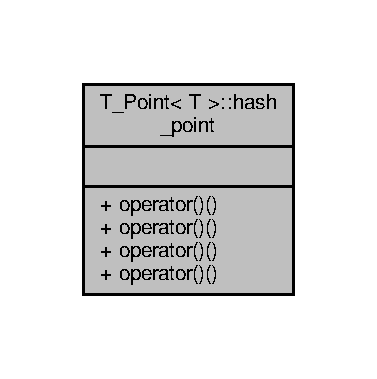
\includegraphics[width=181pt]{structT__Point_1_1hash__point__coll__graph}
\end{center}
\end{figure}
\subsection*{Public Member Functions}
\begin{DoxyCompactItemize}
\item 
std\+::size\+\_\+t \hyperlink{structT__Point_1_1hash__point_a6d41490eb7af074b029db524a80e2e53}{operator()} (const \hyperlink{classT__Point}{T\+\_\+\+Point}$<$ T $>$ \&p) const
\begin{DoxyCompactList}\small\item\em Operator to hash a point. \end{DoxyCompactList}\item 
bool \hyperlink{structT__Point_1_1hash__point_a92f4c83c6538fcb66804d44e944d7b20}{operator()} (const \hyperlink{classT__Point}{T\+\_\+\+Point}$<$ T $>$ \&p1, const \hyperlink{classT__Point}{T\+\_\+\+Point}$<$ T $>$ \&p2) const
\begin{DoxyCompactList}\small\item\em Operator equal need to hash a point. \end{DoxyCompactList}\end{DoxyCompactItemize}


\subsection{Member Function Documentation}
\mbox{\Hypertarget{structT__Point_1_1hash__point_a6d41490eb7af074b029db524a80e2e53}\label{structT__Point_1_1hash__point_a6d41490eb7af074b029db524a80e2e53}} 
\index{T\+\_\+\+Point\+::hash\+\_\+point@{T\+\_\+\+Point\+::hash\+\_\+point}!operator()@{operator()}}
\index{operator()@{operator()}!T\+\_\+\+Point\+::hash\+\_\+point@{T\+\_\+\+Point\+::hash\+\_\+point}}
\subsubsection{\texorpdfstring{operator()()}{operator()()}\hspace{0.1cm}{\footnotesize\ttfamily [1/2]}}
{\footnotesize\ttfamily template$<$typename T$>$ \\
std\+::size\+\_\+t \hyperlink{classT__Point}{T\+\_\+\+Point}$<$ T $>$\+::hash\+\_\+point\+::operator() (\begin{DoxyParamCaption}\item[{const \hyperlink{classT__Point}{T\+\_\+\+Point}$<$ T $>$ \&}]{p }\end{DoxyParamCaption}) const\hspace{0.3cm}{\ttfamily [inline]}}



Operator to hash a point. 


\begin{DoxyParams}{Parameters}
{\em p} & \+: point to hash \\
\hline
\end{DoxyParams}
\begin{DoxyReturn}{Returns}
Return the hash of the point 
\end{DoxyReturn}
\mbox{\Hypertarget{structT__Point_1_1hash__point_a92f4c83c6538fcb66804d44e944d7b20}\label{structT__Point_1_1hash__point_a92f4c83c6538fcb66804d44e944d7b20}} 
\index{T\+\_\+\+Point\+::hash\+\_\+point@{T\+\_\+\+Point\+::hash\+\_\+point}!operator()@{operator()}}
\index{operator()@{operator()}!T\+\_\+\+Point\+::hash\+\_\+point@{T\+\_\+\+Point\+::hash\+\_\+point}}
\subsubsection{\texorpdfstring{operator()()}{operator()()}\hspace{0.1cm}{\footnotesize\ttfamily [2/2]}}
{\footnotesize\ttfamily template$<$typename T$>$ \\
bool \hyperlink{classT__Point}{T\+\_\+\+Point}$<$ T $>$\+::hash\+\_\+point\+::operator() (\begin{DoxyParamCaption}\item[{const \hyperlink{classT__Point}{T\+\_\+\+Point}$<$ T $>$ \&}]{p1,  }\item[{const \hyperlink{classT__Point}{T\+\_\+\+Point}$<$ T $>$ \&}]{p2 }\end{DoxyParamCaption}) const\hspace{0.3cm}{\ttfamily [inline]}}



Operator equal need to hash a point. 


\begin{DoxyParams}{Parameters}
{\em p1} & \+: Point 1 \\
\hline
{\em p2} & \+: Point 2 \\
\hline
\end{DoxyParams}
\begin{DoxyReturn}{Returns}
Return true if p1 and p2 are equals, false otherwise 
\end{DoxyReturn}


The documentation for this struct was generated from the following file\+:\begin{DoxyCompactItemize}
\item 
include/utils/\hyperlink{T__Point_8hpp}{T\+\_\+\+Point.\+hpp}\end{DoxyCompactItemize}

\hypertarget{classI__Drawable}{}\section{I\+\_\+\+Drawable Class Reference}
\label{classI__Drawable}\index{I\+\_\+\+Drawable@{I\+\_\+\+Drawable}}


\hyperlink{classI__Drawable}{I\+\_\+\+Drawable} is everything to i\+Draw.  




{\ttfamily \#include $<$I\+\_\+\+Drawable.\+h$>$}



Inheritance diagram for I\+\_\+\+Drawable\+:\nopagebreak
\begin{figure}[H]
\begin{center}
\leavevmode
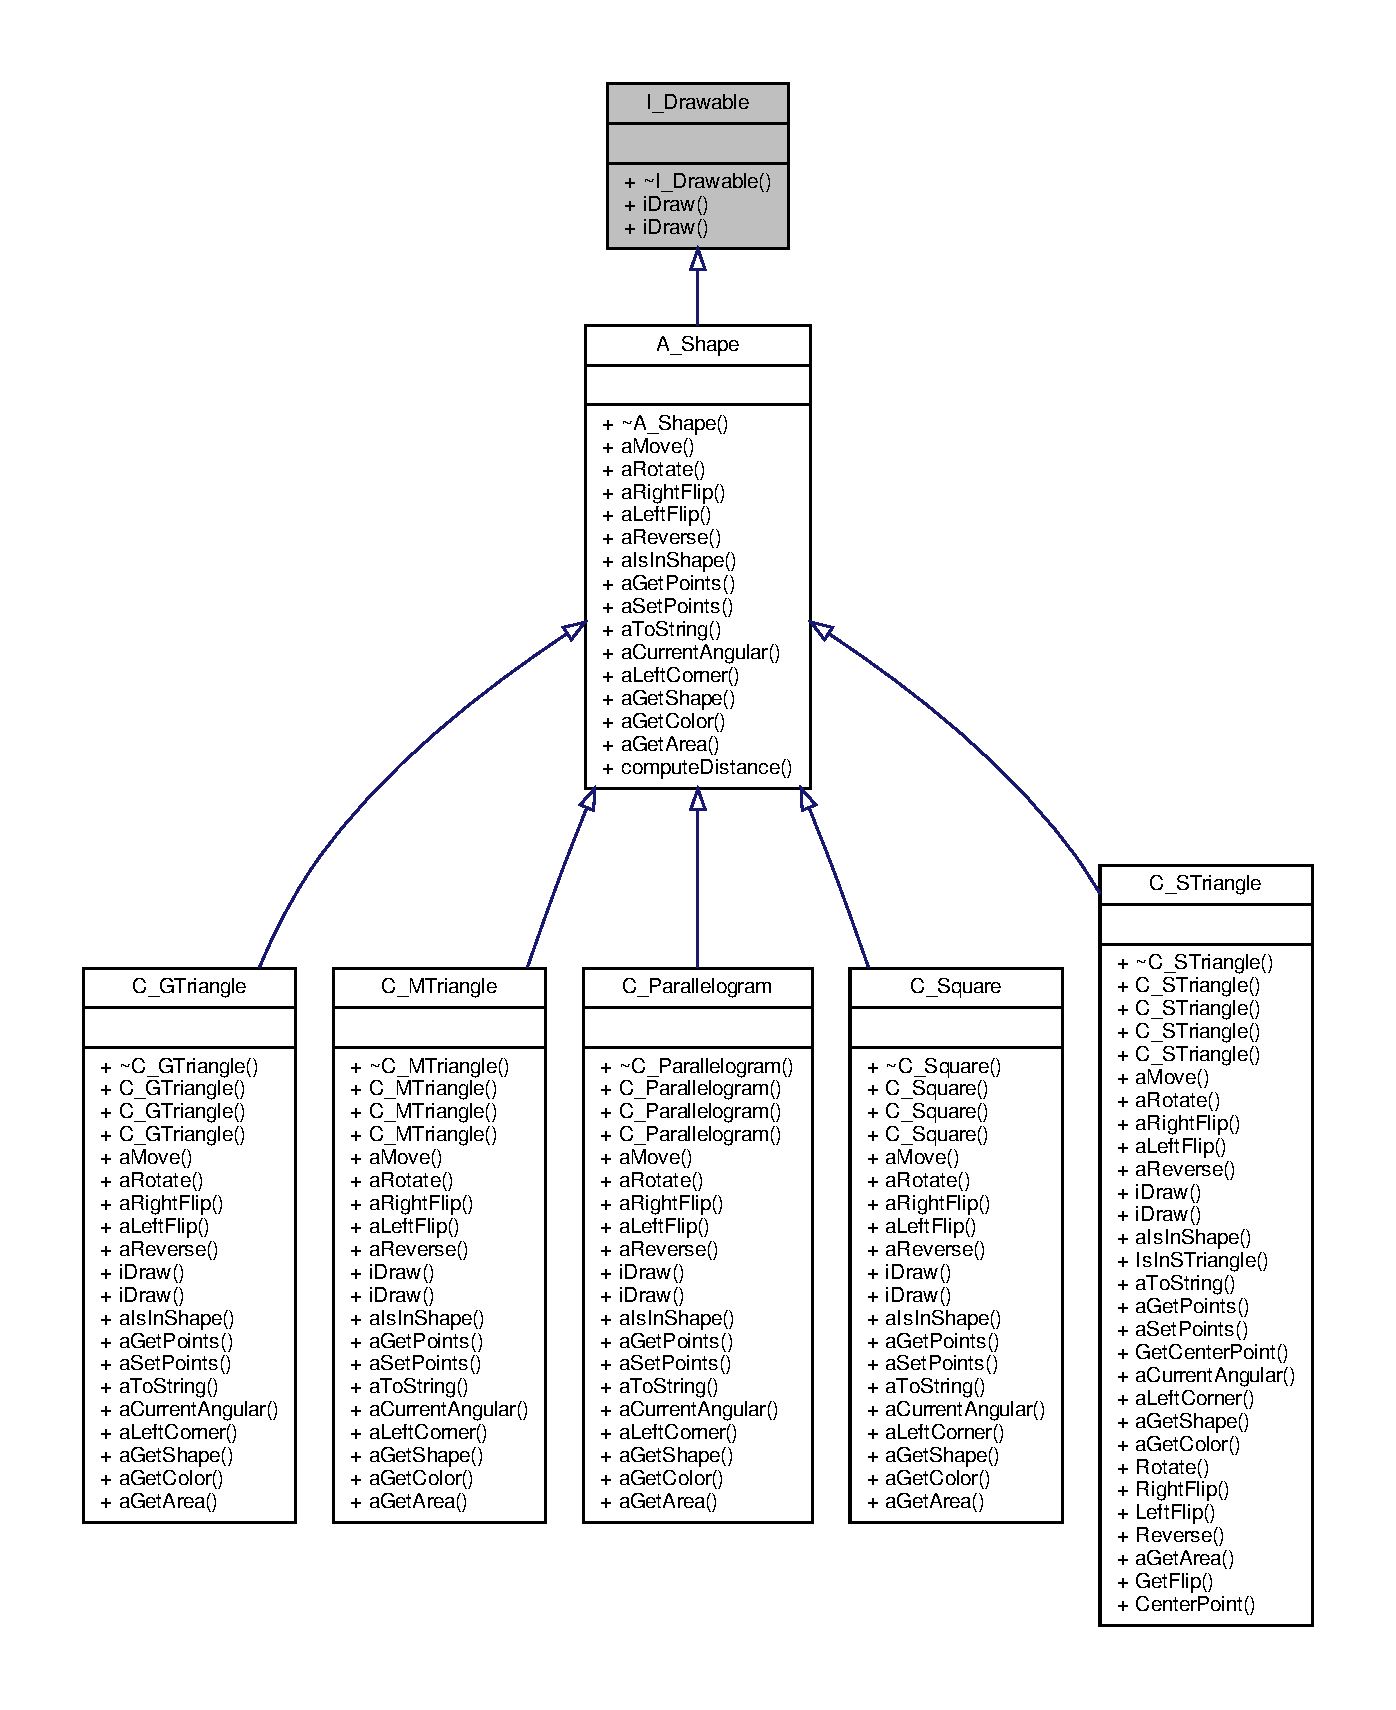
\includegraphics[height=550pt]{classI__Drawable__inherit__graph}
\end{center}
\end{figure}


Collaboration diagram for I\+\_\+\+Drawable\+:\nopagebreak
\begin{figure}[H]
\begin{center}
\leavevmode
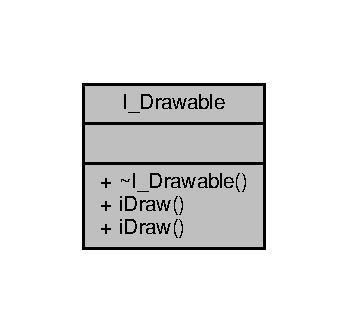
\includegraphics[width=167pt]{classI__Drawable__coll__graph}
\end{center}
\end{figure}
\subsection*{Public Member Functions}
\begin{DoxyCompactItemize}
\item 
\hyperlink{classI__Drawable_a80bfc9f76ccdded97cbcf446d4ace774}{$\sim$\+I\+\_\+\+Drawable} ()=default
\begin{DoxyCompactList}\small\item\em Pure virtual function. Draw everything which needs to be i\+Draw. \end{DoxyCompactList}\item 
virtual void \hyperlink{classI__Drawable_ae24c65000977a805f52ce032321cd86f}{i\+Draw} ()=0
\item 
virtual void \hyperlink{classI__Drawable_a25f6474325614c451a91f019e5fe8010}{i\+Draw} (M\+L\+V\+\_\+\+Color color)=0
\item 
\hyperlink{classI__Drawable_a80bfc9f76ccdded97cbcf446d4ace774}{$\sim$\+I\+\_\+\+Drawable} ()=default
\begin{DoxyCompactList}\small\item\em Pure virtual function. Draw everything which needs to be i\+Draw. \end{DoxyCompactList}\item 
virtual void \hyperlink{classI__Drawable_ae24c65000977a805f52ce032321cd86f}{i\+Draw} ()=0
\item 
virtual void \hyperlink{classI__Drawable_a25f6474325614c451a91f019e5fe8010}{i\+Draw} (M\+L\+V\+\_\+\+Color color)=0
\end{DoxyCompactItemize}


\subsection{Detailed Description}
\hyperlink{classI__Drawable}{I\+\_\+\+Drawable} is everything to i\+Draw. 

This class manage everything drawing 

\subsection{Constructor \& Destructor Documentation}
\mbox{\Hypertarget{classI__Drawable_a80bfc9f76ccdded97cbcf446d4ace774}\label{classI__Drawable_a80bfc9f76ccdded97cbcf446d4ace774}} 
\index{I\+\_\+\+Drawable@{I\+\_\+\+Drawable}!````~I\+\_\+\+Drawable@{$\sim$\+I\+\_\+\+Drawable}}
\index{````~I\+\_\+\+Drawable@{$\sim$\+I\+\_\+\+Drawable}!I\+\_\+\+Drawable@{I\+\_\+\+Drawable}}
\subsubsection{\texorpdfstring{$\sim$\+I\+\_\+\+Drawable()}{~I\_Drawable()}\hspace{0.1cm}{\footnotesize\ttfamily [1/2]}}
{\footnotesize\ttfamily I\+\_\+\+Drawable\+::$\sim$\+I\+\_\+\+Drawable (\begin{DoxyParamCaption}{ }\end{DoxyParamCaption})\hspace{0.3cm}{\ttfamily [default]}}



Pure virtual function. Draw everything which needs to be i\+Draw. 

\mbox{\Hypertarget{classI__Drawable_a80bfc9f76ccdded97cbcf446d4ace774}\label{classI__Drawable_a80bfc9f76ccdded97cbcf446d4ace774}} 
\index{I\+\_\+\+Drawable@{I\+\_\+\+Drawable}!````~I\+\_\+\+Drawable@{$\sim$\+I\+\_\+\+Drawable}}
\index{````~I\+\_\+\+Drawable@{$\sim$\+I\+\_\+\+Drawable}!I\+\_\+\+Drawable@{I\+\_\+\+Drawable}}
\subsubsection{\texorpdfstring{$\sim$\+I\+\_\+\+Drawable()}{~I\_Drawable()}\hspace{0.1cm}{\footnotesize\ttfamily [2/2]}}
{\footnotesize\ttfamily I\+\_\+\+Drawable\+::$\sim$\+I\+\_\+\+Drawable (\begin{DoxyParamCaption}{ }\end{DoxyParamCaption})\hspace{0.3cm}{\ttfamily [default]}}



Pure virtual function. Draw everything which needs to be i\+Draw. 



\subsection{Member Function Documentation}
\mbox{\Hypertarget{classI__Drawable_ae24c65000977a805f52ce032321cd86f}\label{classI__Drawable_ae24c65000977a805f52ce032321cd86f}} 
\index{I\+\_\+\+Drawable@{I\+\_\+\+Drawable}!i\+Draw@{i\+Draw}}
\index{i\+Draw@{i\+Draw}!I\+\_\+\+Drawable@{I\+\_\+\+Drawable}}
\subsubsection{\texorpdfstring{i\+Draw()}{iDraw()}\hspace{0.1cm}{\footnotesize\ttfamily [1/4]}}
{\footnotesize\ttfamily virtual void I\+\_\+\+Drawable\+::i\+Draw (\begin{DoxyParamCaption}{ }\end{DoxyParamCaption})\hspace{0.3cm}{\ttfamily [pure virtual]}}



Implemented in \hyperlink{classC__STriangle_a7297480fe52b58654d81e2e70fbb237d}{C\+\_\+\+S\+Triangle}, \hyperlink{classC__STriangle_a7297480fe52b58654d81e2e70fbb237d}{C\+\_\+\+S\+Triangle}, \hyperlink{classC__Parallelogram_a6d43cc787a39def68c7b7de4a33caf5e}{C\+\_\+\+Parallelogram}, \hyperlink{classC__Parallelogram_a6d43cc787a39def68c7b7de4a33caf5e}{C\+\_\+\+Parallelogram}, \hyperlink{classC__MTriangle_ae75dd212f0b580664affc740945c8d0b}{C\+\_\+\+M\+Triangle}, \hyperlink{classC__Square_ae6c51a7720576bcbb94b52584552df28}{C\+\_\+\+Square}, \hyperlink{classC__MTriangle_ae75dd212f0b580664affc740945c8d0b}{C\+\_\+\+M\+Triangle}, \hyperlink{classC__Square_ae6c51a7720576bcbb94b52584552df28}{C\+\_\+\+Square}, \hyperlink{classC__GTriangle_a53abbd8cd622323fc2f3b80ce91cfde9}{C\+\_\+\+G\+Triangle}, and \hyperlink{classC__GTriangle_a53abbd8cd622323fc2f3b80ce91cfde9}{C\+\_\+\+G\+Triangle}.

\mbox{\Hypertarget{classI__Drawable_ae24c65000977a805f52ce032321cd86f}\label{classI__Drawable_ae24c65000977a805f52ce032321cd86f}} 
\index{I\+\_\+\+Drawable@{I\+\_\+\+Drawable}!i\+Draw@{i\+Draw}}
\index{i\+Draw@{i\+Draw}!I\+\_\+\+Drawable@{I\+\_\+\+Drawable}}
\subsubsection{\texorpdfstring{i\+Draw()}{iDraw()}\hspace{0.1cm}{\footnotesize\ttfamily [2/4]}}
{\footnotesize\ttfamily virtual void I\+\_\+\+Drawable\+::i\+Draw (\begin{DoxyParamCaption}{ }\end{DoxyParamCaption})\hspace{0.3cm}{\ttfamily [pure virtual]}}



Implemented in \hyperlink{classC__STriangle_a7297480fe52b58654d81e2e70fbb237d}{C\+\_\+\+S\+Triangle}, \hyperlink{classC__STriangle_a7297480fe52b58654d81e2e70fbb237d}{C\+\_\+\+S\+Triangle}, \hyperlink{classC__Parallelogram_a6d43cc787a39def68c7b7de4a33caf5e}{C\+\_\+\+Parallelogram}, \hyperlink{classC__Parallelogram_a6d43cc787a39def68c7b7de4a33caf5e}{C\+\_\+\+Parallelogram}, \hyperlink{classC__MTriangle_ae75dd212f0b580664affc740945c8d0b}{C\+\_\+\+M\+Triangle}, \hyperlink{classC__Square_ae6c51a7720576bcbb94b52584552df28}{C\+\_\+\+Square}, \hyperlink{classC__MTriangle_ae75dd212f0b580664affc740945c8d0b}{C\+\_\+\+M\+Triangle}, \hyperlink{classC__Square_ae6c51a7720576bcbb94b52584552df28}{C\+\_\+\+Square}, \hyperlink{classC__GTriangle_a53abbd8cd622323fc2f3b80ce91cfde9}{C\+\_\+\+G\+Triangle}, and \hyperlink{classC__GTriangle_a53abbd8cd622323fc2f3b80ce91cfde9}{C\+\_\+\+G\+Triangle}.

\mbox{\Hypertarget{classI__Drawable_a25f6474325614c451a91f019e5fe8010}\label{classI__Drawable_a25f6474325614c451a91f019e5fe8010}} 
\index{I\+\_\+\+Drawable@{I\+\_\+\+Drawable}!i\+Draw@{i\+Draw}}
\index{i\+Draw@{i\+Draw}!I\+\_\+\+Drawable@{I\+\_\+\+Drawable}}
\subsubsection{\texorpdfstring{i\+Draw()}{iDraw()}\hspace{0.1cm}{\footnotesize\ttfamily [3/4]}}
{\footnotesize\ttfamily virtual void I\+\_\+\+Drawable\+::i\+Draw (\begin{DoxyParamCaption}\item[{M\+L\+V\+\_\+\+Color}]{color }\end{DoxyParamCaption})\hspace{0.3cm}{\ttfamily [pure virtual]}}



Implemented in \hyperlink{classC__STriangle_ad003b932a467de60b814d897fda38390}{C\+\_\+\+S\+Triangle}, \hyperlink{classC__STriangle_ad003b932a467de60b814d897fda38390}{C\+\_\+\+S\+Triangle}, \hyperlink{classC__Parallelogram_a044ce6d1042ea93589a38f4686489862}{C\+\_\+\+Parallelogram}, \hyperlink{classC__Parallelogram_a044ce6d1042ea93589a38f4686489862}{C\+\_\+\+Parallelogram}, \hyperlink{classC__MTriangle_a049e6026145865387db4244678336784}{C\+\_\+\+M\+Triangle}, \hyperlink{classC__Square_a47a80c25bbeda17f17a8230127b4a5ed}{C\+\_\+\+Square}, \hyperlink{classC__MTriangle_a049e6026145865387db4244678336784}{C\+\_\+\+M\+Triangle}, \hyperlink{classC__Square_a47a80c25bbeda17f17a8230127b4a5ed}{C\+\_\+\+Square}, \hyperlink{classC__GTriangle_a9cfd20cb1d19e6c92bd217c470c86405}{C\+\_\+\+G\+Triangle}, and \hyperlink{classC__GTriangle_a9cfd20cb1d19e6c92bd217c470c86405}{C\+\_\+\+G\+Triangle}.

\mbox{\Hypertarget{classI__Drawable_a25f6474325614c451a91f019e5fe8010}\label{classI__Drawable_a25f6474325614c451a91f019e5fe8010}} 
\index{I\+\_\+\+Drawable@{I\+\_\+\+Drawable}!i\+Draw@{i\+Draw}}
\index{i\+Draw@{i\+Draw}!I\+\_\+\+Drawable@{I\+\_\+\+Drawable}}
\subsubsection{\texorpdfstring{i\+Draw()}{iDraw()}\hspace{0.1cm}{\footnotesize\ttfamily [4/4]}}
{\footnotesize\ttfamily virtual void I\+\_\+\+Drawable\+::i\+Draw (\begin{DoxyParamCaption}\item[{M\+L\+V\+\_\+\+Color}]{color }\end{DoxyParamCaption})\hspace{0.3cm}{\ttfamily [pure virtual]}}



Implemented in \hyperlink{classC__STriangle_ad003b932a467de60b814d897fda38390}{C\+\_\+\+S\+Triangle}, \hyperlink{classC__STriangle_ad003b932a467de60b814d897fda38390}{C\+\_\+\+S\+Triangle}, \hyperlink{classC__Parallelogram_a044ce6d1042ea93589a38f4686489862}{C\+\_\+\+Parallelogram}, \hyperlink{classC__Parallelogram_a044ce6d1042ea93589a38f4686489862}{C\+\_\+\+Parallelogram}, \hyperlink{classC__MTriangle_a049e6026145865387db4244678336784}{C\+\_\+\+M\+Triangle}, \hyperlink{classC__Square_a47a80c25bbeda17f17a8230127b4a5ed}{C\+\_\+\+Square}, \hyperlink{classC__MTriangle_a049e6026145865387db4244678336784}{C\+\_\+\+M\+Triangle}, \hyperlink{classC__Square_a47a80c25bbeda17f17a8230127b4a5ed}{C\+\_\+\+Square}, \hyperlink{classC__GTriangle_a9cfd20cb1d19e6c92bd217c470c86405}{C\+\_\+\+G\+Triangle}, and \hyperlink{classC__GTriangle_a9cfd20cb1d19e6c92bd217c470c86405}{C\+\_\+\+G\+Triangle}.



The documentation for this class was generated from the following file\+:\begin{DoxyCompactItemize}
\item 
include/drawable/\hyperlink{drawable_2I__Drawable_8h}{I\+\_\+\+Drawable.\+h}\end{DoxyCompactItemize}

\hypertarget{structStruct}{}\section{Struct Struct Reference}
\label{structStruct}\index{Struct@{Struct}}


Hash a Point$<$\+T$>$ to hash a point with Point$<$\+T$>$  




\subsection{Detailed Description}
Hash a Point$<$\+T$>$ to hash a point with Point$<$\+T$>$ 

The documentation for this struct was generated from the following file\+:\begin{DoxyCompactItemize}
\item 
include/utils/\hyperlink{Point_8hpp}{Point.\+hpp}\end{DoxyCompactItemize}

\hypertarget{classT__Point}{}\section{T\+\_\+\+Point$<$ T $>$ Class Template Reference}
\label{classT__Point}\index{T\+\_\+\+Point$<$ T $>$@{T\+\_\+\+Point$<$ T $>$}}


Class of a \hyperlink{classT__Point}{T\+\_\+\+Point}.  




{\ttfamily \#include $<$T\+\_\+\+Point.\+hpp$>$}



Inheritance diagram for T\+\_\+\+Point$<$ T $>$\+:\nopagebreak
\begin{figure}[H]
\begin{center}
\leavevmode
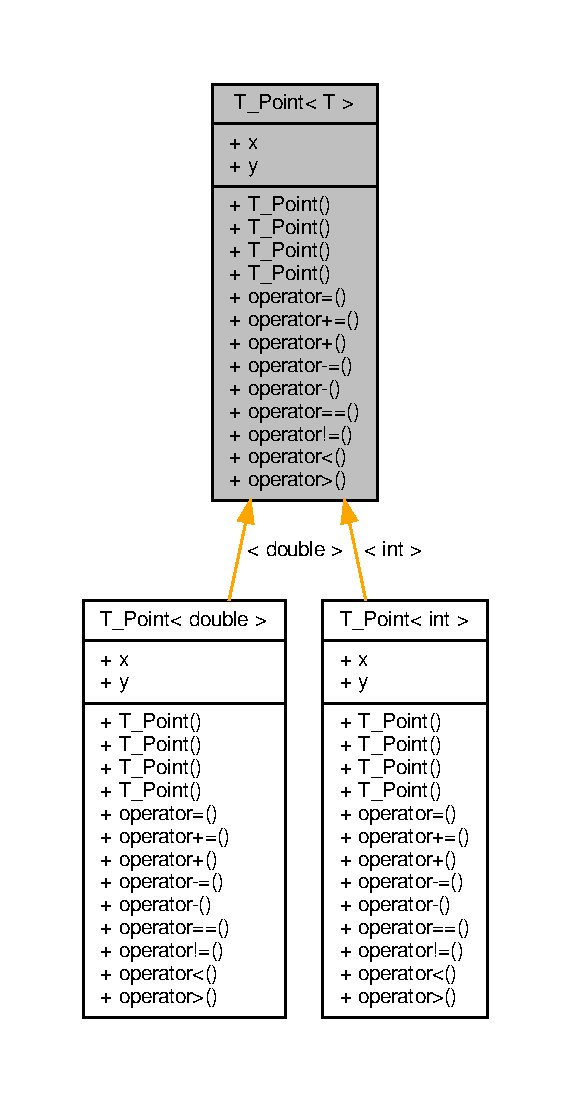
\includegraphics[height=550pt]{classT__Point__inherit__graph}
\end{center}
\end{figure}


Collaboration diagram for T\+\_\+\+Point$<$ T $>$\+:\nopagebreak
\begin{figure}[H]
\begin{center}
\leavevmode
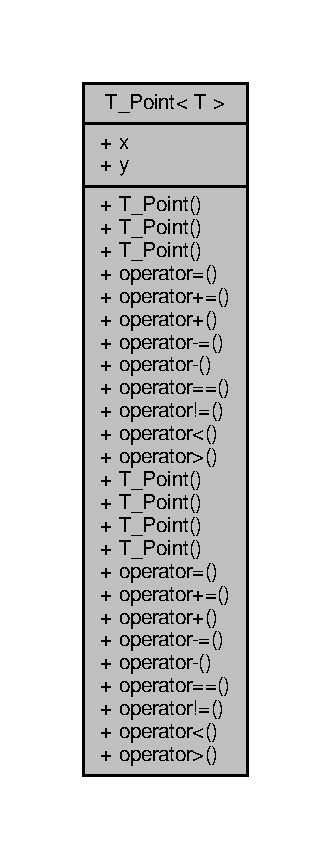
\includegraphics[width=159pt]{classT__Point__coll__graph}
\end{center}
\end{figure}
\subsection*{Classes}
\begin{DoxyCompactItemize}
\item 
struct \hyperlink{structT__Point_1_1hash__point}{hash\+\_\+point}
\end{DoxyCompactItemize}
\subsection*{Public Member Functions}
\begin{DoxyCompactItemize}
\item 
constexpr \hyperlink{classT__Point_af313da04154273b9a75d66e9950359ea}{T\+\_\+\+Point} (const \hyperlink{classT__Point}{T\+\_\+\+Point}$<$ T $>$ \&p)=default
\item 
\hyperlink{classT__Point_a61017b12d3c2aa88a242dbbc57733413}{T\+\_\+\+Point} ()
\begin{DoxyCompactList}\small\item\em Constructor for a point with initialisation list. \end{DoxyCompactList}\item 
\hyperlink{classT__Point_a12f2ef3c5f10e162dcb6385bbfbfae58}{T\+\_\+\+Point} (const T \&\+\_\+x, const T \&\+\_\+y)
\begin{DoxyCompactList}\small\item\em Constructor of a point with move semantic. \end{DoxyCompactList}\item 
\hyperlink{classT__Point}{T\+\_\+\+Point} \& \hyperlink{classT__Point_a13fbb5646f2333aa41194d648423e10f}{operator=} (const \hyperlink{classT__Point}{T\+\_\+\+Point}$<$ T $>$ \&p)
\begin{DoxyCompactList}\small\item\em Operator = of a point. \end{DoxyCompactList}\item 
\hyperlink{classT__Point}{T\+\_\+\+Point} \& \hyperlink{classT__Point_a4fa7b8ceb837c81e608d5ddad0f1ffe7}{operator+=} (const \hyperlink{classT__Point}{T\+\_\+\+Point}$<$ T $>$ \&p)
\begin{DoxyCompactList}\small\item\em Operator +=. \end{DoxyCompactList}\item 
\hyperlink{classT__Point}{T\+\_\+\+Point} \hyperlink{classT__Point_a1f94a7a19cc8711e7784f700ea59297a}{operator+} (const \hyperlink{classT__Point}{T\+\_\+\+Point}$<$ T $>$ \&p)
\begin{DoxyCompactList}\small\item\em Operator +. \end{DoxyCompactList}\item 
\hyperlink{classT__Point}{T\+\_\+\+Point} \& \hyperlink{classT__Point_aa438de3090999e1f24f0de58dc5171a0}{operator-\/=} (const \hyperlink{classT__Point}{T\+\_\+\+Point}$<$ T $>$ \&p)
\begin{DoxyCompactList}\small\item\em Operator -\/=. \end{DoxyCompactList}\item 
\hyperlink{classT__Point}{T\+\_\+\+Point} \hyperlink{classT__Point_a4a3671d0a9763b3e749c799294ebb1ca}{operator-\/} (const \hyperlink{classT__Point}{T\+\_\+\+Point}$<$ T $>$ \&p)
\begin{DoxyCompactList}\small\item\em Operator -\/. \end{DoxyCompactList}\item 
bool \hyperlink{classT__Point_a83c15f53049523cc75c23350ceb4832a}{operator==} (const \hyperlink{classT__Point}{T\+\_\+\+Point}$<$ T $>$ \&p) const
\begin{DoxyCompactList}\small\item\em Operator == of a point. \end{DoxyCompactList}\item 
bool \hyperlink{classT__Point_ab92f1605c6f5008b42105b4c7a7fc1b2}{operator!=} (const \hyperlink{classT__Point}{T\+\_\+\+Point}$<$ T $>$ \&p) const
\begin{DoxyCompactList}\small\item\em Operator != of a point. \end{DoxyCompactList}\item 
bool \hyperlink{classT__Point_a95cb559fe5888b44481f6ad3aebabefe}{operator$<$} (const \hyperlink{classT__Point}{T\+\_\+\+Point}$<$ T $>$ \&p) const
\begin{DoxyCompactList}\small\item\em Operator $<$ of a point. \end{DoxyCompactList}\item 
bool \hyperlink{classT__Point_a0a9956de8ab7c8dccf35b78c43aedefd}{operator$>$} (const \hyperlink{classT__Point}{T\+\_\+\+Point}$<$ T $>$ \&p) const
\begin{DoxyCompactList}\small\item\em Operator $>$ of a point. \end{DoxyCompactList}\item 
constexpr \hyperlink{classT__Point_af313da04154273b9a75d66e9950359ea}{T\+\_\+\+Point} (const \hyperlink{classT__Point}{T\+\_\+\+Point}$<$ T $>$ \&p)=default
\item 
\hyperlink{classT__Point_a61017b12d3c2aa88a242dbbc57733413}{T\+\_\+\+Point} ()
\begin{DoxyCompactList}\small\item\em Constructor for a point with initialisation list. \end{DoxyCompactList}\item 
\hyperlink{classT__Point_af6c471d7e5547576a6c379930b9d1d35}{T\+\_\+\+Point} (const \hyperlink{classT__Point}{T\+\_\+\+Point}$<$ T $>$ \&\&p) noexcept
\begin{DoxyCompactList}\small\item\em Constructor of a point with move semantic. \end{DoxyCompactList}\item 
\hyperlink{classT__Point_a12f2ef3c5f10e162dcb6385bbfbfae58}{T\+\_\+\+Point} (const T \&\+\_\+x, const T \&\+\_\+y)
\begin{DoxyCompactList}\small\item\em Constructor for a point. Requires a X and a Y coordinate. \end{DoxyCompactList}\item 
\hyperlink{classT__Point}{T\+\_\+\+Point} \& \hyperlink{classT__Point_a13fbb5646f2333aa41194d648423e10f}{operator=} (const \hyperlink{classT__Point}{T\+\_\+\+Point}$<$ T $>$ \&p)
\begin{DoxyCompactList}\small\item\em Operator = of a point. \end{DoxyCompactList}\item 
\hyperlink{classT__Point}{T\+\_\+\+Point} \& \hyperlink{classT__Point_a4fa7b8ceb837c81e608d5ddad0f1ffe7}{operator+=} (const \hyperlink{classT__Point}{T\+\_\+\+Point}$<$ T $>$ \&p)
\begin{DoxyCompactList}\small\item\em Operator +=. \end{DoxyCompactList}\item 
\hyperlink{classT__Point}{T\+\_\+\+Point} \hyperlink{classT__Point_a1f94a7a19cc8711e7784f700ea59297a}{operator+} (const \hyperlink{classT__Point}{T\+\_\+\+Point}$<$ T $>$ \&p)
\begin{DoxyCompactList}\small\item\em Operator +. \end{DoxyCompactList}\item 
\hyperlink{classT__Point}{T\+\_\+\+Point} \& \hyperlink{classT__Point_aa438de3090999e1f24f0de58dc5171a0}{operator-\/=} (const \hyperlink{classT__Point}{T\+\_\+\+Point}$<$ T $>$ \&p)
\begin{DoxyCompactList}\small\item\em Operator -\/=. \end{DoxyCompactList}\item 
\hyperlink{classT__Point}{T\+\_\+\+Point} \hyperlink{classT__Point_a4a3671d0a9763b3e749c799294ebb1ca}{operator-\/} (const \hyperlink{classT__Point}{T\+\_\+\+Point}$<$ T $>$ \&p)
\begin{DoxyCompactList}\small\item\em Operator -\/. \end{DoxyCompactList}\item 
bool \hyperlink{classT__Point_a83c15f53049523cc75c23350ceb4832a}{operator==} (const \hyperlink{classT__Point}{T\+\_\+\+Point}$<$ T $>$ \&p) const
\begin{DoxyCompactList}\small\item\em Operator == of a point. \end{DoxyCompactList}\item 
bool \hyperlink{classT__Point_ab92f1605c6f5008b42105b4c7a7fc1b2}{operator!=} (const \hyperlink{classT__Point}{T\+\_\+\+Point}$<$ T $>$ \&p) const
\begin{DoxyCompactList}\small\item\em Operator != of a point. \end{DoxyCompactList}\item 
bool \hyperlink{classT__Point_a95cb559fe5888b44481f6ad3aebabefe}{operator$<$} (const \hyperlink{classT__Point}{T\+\_\+\+Point}$<$ T $>$ \&p) const
\begin{DoxyCompactList}\small\item\em Operator $<$ of a point. \end{DoxyCompactList}\item 
bool \hyperlink{classT__Point_a0a9956de8ab7c8dccf35b78c43aedefd}{operator$>$} (const \hyperlink{classT__Point}{T\+\_\+\+Point}$<$ T $>$ \&p) const
\begin{DoxyCompactList}\small\item\em Operator $>$ of a point. \end{DoxyCompactList}\end{DoxyCompactItemize}
\subsection*{Public Attributes}
\begin{DoxyCompactItemize}
\item 
T \hyperlink{classT__Point_a45cc1c670a8d9bc786a38428cdce4bd2}{x}
\item 
T \hyperlink{classT__Point_a28da35a974844bdb3509a90345d3c1f9}{y}
\end{DoxyCompactItemize}


\subsection{Detailed Description}
\subsubsection*{template$<$typename T$>$\newline
class T\+\_\+\+Point$<$ T $>$}

Class of a \hyperlink{classT__Point}{T\+\_\+\+Point}. 


\begin{DoxyTemplParams}{Template Parameters}
{\em T} & \+: Template parameter This class manage everything about a point \\
\hline
\end{DoxyTemplParams}


\subsection{Constructor \& Destructor Documentation}
\mbox{\Hypertarget{classT__Point_af313da04154273b9a75d66e9950359ea}\label{classT__Point_af313da04154273b9a75d66e9950359ea}} 
\index{T\+\_\+\+Point@{T\+\_\+\+Point}!T\+\_\+\+Point@{T\+\_\+\+Point}}
\index{T\+\_\+\+Point@{T\+\_\+\+Point}!T\+\_\+\+Point@{T\+\_\+\+Point}}
\subsubsection{\texorpdfstring{T\+\_\+\+Point()}{T\_Point()}\hspace{0.1cm}{\footnotesize\ttfamily [1/7]}}
{\footnotesize\ttfamily template$<$typename T$>$ \\
constexpr \hyperlink{classT__Point}{T\+\_\+\+Point}$<$ T $>$\+::\hyperlink{classT__Point}{T\+\_\+\+Point} (\begin{DoxyParamCaption}\item[{const \hyperlink{classT__Point}{T\+\_\+\+Point}$<$ T $>$ \&}]{p }\end{DoxyParamCaption})\hspace{0.3cm}{\ttfamily [default]}}

\mbox{\Hypertarget{classT__Point_a61017b12d3c2aa88a242dbbc57733413}\label{classT__Point_a61017b12d3c2aa88a242dbbc57733413}} 
\index{T\+\_\+\+Point@{T\+\_\+\+Point}!T\+\_\+\+Point@{T\+\_\+\+Point}}
\index{T\+\_\+\+Point@{T\+\_\+\+Point}!T\+\_\+\+Point@{T\+\_\+\+Point}}
\subsubsection{\texorpdfstring{T\+\_\+\+Point()}{T\_Point()}\hspace{0.1cm}{\footnotesize\ttfamily [2/7]}}
{\footnotesize\ttfamily template$<$typename T$>$ \\
\hyperlink{classT__Point}{T\+\_\+\+Point}$<$ T $>$\+::\hyperlink{classT__Point}{T\+\_\+\+Point} (\begin{DoxyParamCaption}{ }\end{DoxyParamCaption})\hspace{0.3cm}{\ttfamily [inline]}}



Constructor for a point with initialisation list. 

\mbox{\Hypertarget{classT__Point_a12f2ef3c5f10e162dcb6385bbfbfae58}\label{classT__Point_a12f2ef3c5f10e162dcb6385bbfbfae58}} 
\index{T\+\_\+\+Point@{T\+\_\+\+Point}!T\+\_\+\+Point@{T\+\_\+\+Point}}
\index{T\+\_\+\+Point@{T\+\_\+\+Point}!T\+\_\+\+Point@{T\+\_\+\+Point}}
\subsubsection{\texorpdfstring{T\+\_\+\+Point()}{T\_Point()}\hspace{0.1cm}{\footnotesize\ttfamily [3/7]}}
{\footnotesize\ttfamily template$<$typename T$>$ \\
\hyperlink{classT__Point}{T\+\_\+\+Point}$<$ T $>$\+::\hyperlink{classT__Point}{T\+\_\+\+Point} (\begin{DoxyParamCaption}\item[{const T \&}]{\+\_\+x,  }\item[{const T \&}]{\+\_\+y }\end{DoxyParamCaption})\hspace{0.3cm}{\ttfamily [inline]}}



Constructor of a point with move semantic. 


\begin{DoxyParams}{Parameters}
{\em p} & \+: Point to move\\
\hline
\end{DoxyParams}
Constructor for a point. Requires a X and a Y coordinate 
\begin{DoxyParams}{Parameters}
{\em \+\_\+x} & \+: Template X coordinate \\
\hline
{\em \+\_\+y} & \+: Template Y coordinate \\
\hline
\end{DoxyParams}
\mbox{\Hypertarget{classT__Point_af313da04154273b9a75d66e9950359ea}\label{classT__Point_af313da04154273b9a75d66e9950359ea}} 
\index{T\+\_\+\+Point@{T\+\_\+\+Point}!T\+\_\+\+Point@{T\+\_\+\+Point}}
\index{T\+\_\+\+Point@{T\+\_\+\+Point}!T\+\_\+\+Point@{T\+\_\+\+Point}}
\subsubsection{\texorpdfstring{T\+\_\+\+Point()}{T\_Point()}\hspace{0.1cm}{\footnotesize\ttfamily [4/7]}}
{\footnotesize\ttfamily template$<$typename T$>$ \\
constexpr \hyperlink{classT__Point}{T\+\_\+\+Point}$<$ T $>$\+::\hyperlink{classT__Point}{T\+\_\+\+Point} (\begin{DoxyParamCaption}\item[{const \hyperlink{classT__Point}{T\+\_\+\+Point}$<$ T $>$ \&}]{p }\end{DoxyParamCaption})\hspace{0.3cm}{\ttfamily [default]}}

\mbox{\Hypertarget{classT__Point_a61017b12d3c2aa88a242dbbc57733413}\label{classT__Point_a61017b12d3c2aa88a242dbbc57733413}} 
\index{T\+\_\+\+Point@{T\+\_\+\+Point}!T\+\_\+\+Point@{T\+\_\+\+Point}}
\index{T\+\_\+\+Point@{T\+\_\+\+Point}!T\+\_\+\+Point@{T\+\_\+\+Point}}
\subsubsection{\texorpdfstring{T\+\_\+\+Point()}{T\_Point()}\hspace{0.1cm}{\footnotesize\ttfamily [5/7]}}
{\footnotesize\ttfamily template$<$typename T$>$ \\
\hyperlink{classT__Point}{T\+\_\+\+Point}$<$ T $>$\+::\hyperlink{classT__Point}{T\+\_\+\+Point} (\begin{DoxyParamCaption}{ }\end{DoxyParamCaption})\hspace{0.3cm}{\ttfamily [inline]}}



Constructor for a point with initialisation list. 

\mbox{\Hypertarget{classT__Point_af6c471d7e5547576a6c379930b9d1d35}\label{classT__Point_af6c471d7e5547576a6c379930b9d1d35}} 
\index{T\+\_\+\+Point@{T\+\_\+\+Point}!T\+\_\+\+Point@{T\+\_\+\+Point}}
\index{T\+\_\+\+Point@{T\+\_\+\+Point}!T\+\_\+\+Point@{T\+\_\+\+Point}}
\subsubsection{\texorpdfstring{T\+\_\+\+Point()}{T\_Point()}\hspace{0.1cm}{\footnotesize\ttfamily [6/7]}}
{\footnotesize\ttfamily template$<$typename T$>$ \\
\hyperlink{classT__Point}{T\+\_\+\+Point}$<$ T $>$\+::\hyperlink{classT__Point}{T\+\_\+\+Point} (\begin{DoxyParamCaption}\item[{const \hyperlink{classT__Point}{T\+\_\+\+Point}$<$ T $>$ \&\&}]{p }\end{DoxyParamCaption})\hspace{0.3cm}{\ttfamily [inline]}, {\ttfamily [noexcept]}}



Constructor of a point with move semantic. 


\begin{DoxyParams}{Parameters}
{\em p} & \+: Point to move \\
\hline
\end{DoxyParams}
\mbox{\Hypertarget{classT__Point_a12f2ef3c5f10e162dcb6385bbfbfae58}\label{classT__Point_a12f2ef3c5f10e162dcb6385bbfbfae58}} 
\index{T\+\_\+\+Point@{T\+\_\+\+Point}!T\+\_\+\+Point@{T\+\_\+\+Point}}
\index{T\+\_\+\+Point@{T\+\_\+\+Point}!T\+\_\+\+Point@{T\+\_\+\+Point}}
\subsubsection{\texorpdfstring{T\+\_\+\+Point()}{T\_Point()}\hspace{0.1cm}{\footnotesize\ttfamily [7/7]}}
{\footnotesize\ttfamily template$<$typename T$>$ \\
\hyperlink{classT__Point}{T\+\_\+\+Point}$<$ T $>$\+::\hyperlink{classT__Point}{T\+\_\+\+Point} (\begin{DoxyParamCaption}\item[{const T \&}]{\+\_\+x,  }\item[{const T \&}]{\+\_\+y }\end{DoxyParamCaption})\hspace{0.3cm}{\ttfamily [inline]}}



Constructor for a point. Requires a X and a Y coordinate. 


\begin{DoxyParams}{Parameters}
{\em \+\_\+x} & \+: Template X coordinate \\
\hline
{\em \+\_\+y} & \+: Template Y coordinate \\
\hline
\end{DoxyParams}


\subsection{Member Function Documentation}
\mbox{\Hypertarget{classT__Point_ab92f1605c6f5008b42105b4c7a7fc1b2}\label{classT__Point_ab92f1605c6f5008b42105b4c7a7fc1b2}} 
\index{T\+\_\+\+Point@{T\+\_\+\+Point}!operator"!=@{operator"!=}}
\index{operator"!=@{operator"!=}!T\+\_\+\+Point@{T\+\_\+\+Point}}
\subsubsection{\texorpdfstring{operator"!=()}{operator!=()}\hspace{0.1cm}{\footnotesize\ttfamily [1/2]}}
{\footnotesize\ttfamily template$<$typename T$>$ \\
bool \hyperlink{classT__Point}{T\+\_\+\+Point}$<$ T $>$\+::operator!= (\begin{DoxyParamCaption}\item[{const \hyperlink{classT__Point}{T\+\_\+\+Point}$<$ T $>$ \&}]{p }\end{DoxyParamCaption}) const\hspace{0.3cm}{\ttfamily [inline]}}



Operator != of a point. 


\begin{DoxyParams}{Parameters}
{\em p} & \+: \hyperlink{classT__Point}{T\+\_\+\+Point} to compare \\
\hline
\end{DoxyParams}
\begin{DoxyReturn}{Returns}
Return True if the point is different, false if not 
\end{DoxyReturn}
\mbox{\Hypertarget{classT__Point_ab92f1605c6f5008b42105b4c7a7fc1b2}\label{classT__Point_ab92f1605c6f5008b42105b4c7a7fc1b2}} 
\index{T\+\_\+\+Point@{T\+\_\+\+Point}!operator"!=@{operator"!=}}
\index{operator"!=@{operator"!=}!T\+\_\+\+Point@{T\+\_\+\+Point}}
\subsubsection{\texorpdfstring{operator"!=()}{operator!=()}\hspace{0.1cm}{\footnotesize\ttfamily [2/2]}}
{\footnotesize\ttfamily template$<$typename T$>$ \\
bool \hyperlink{classT__Point}{T\+\_\+\+Point}$<$ T $>$\+::operator!= (\begin{DoxyParamCaption}\item[{const \hyperlink{classT__Point}{T\+\_\+\+Point}$<$ T $>$ \&}]{p }\end{DoxyParamCaption}) const\hspace{0.3cm}{\ttfamily [inline]}}



Operator != of a point. 


\begin{DoxyParams}{Parameters}
{\em p} & \+: \hyperlink{classT__Point}{T\+\_\+\+Point} to compare \\
\hline
\end{DoxyParams}
\begin{DoxyReturn}{Returns}
Return True if the point is different, false if not 
\end{DoxyReturn}
\mbox{\Hypertarget{classT__Point_a1f94a7a19cc8711e7784f700ea59297a}\label{classT__Point_a1f94a7a19cc8711e7784f700ea59297a}} 
\index{T\+\_\+\+Point@{T\+\_\+\+Point}!operator+@{operator+}}
\index{operator+@{operator+}!T\+\_\+\+Point@{T\+\_\+\+Point}}
\subsubsection{\texorpdfstring{operator+()}{operator+()}\hspace{0.1cm}{\footnotesize\ttfamily [1/2]}}
{\footnotesize\ttfamily template$<$typename T$>$ \\
\hyperlink{classT__Point}{T\+\_\+\+Point} \hyperlink{classT__Point}{T\+\_\+\+Point}$<$ T $>$\+::operator+ (\begin{DoxyParamCaption}\item[{const \hyperlink{classT__Point}{T\+\_\+\+Point}$<$ T $>$ \&}]{p }\end{DoxyParamCaption})\hspace{0.3cm}{\ttfamily [inline]}}



Operator +. 


\begin{DoxyParams}{Parameters}
{\em p} & \+: Point \\
\hline
\end{DoxyParams}
\begin{DoxyReturn}{Returns}
Return the behavior when a point is add by another one 
\end{DoxyReturn}
\mbox{\Hypertarget{classT__Point_a1f94a7a19cc8711e7784f700ea59297a}\label{classT__Point_a1f94a7a19cc8711e7784f700ea59297a}} 
\index{T\+\_\+\+Point@{T\+\_\+\+Point}!operator+@{operator+}}
\index{operator+@{operator+}!T\+\_\+\+Point@{T\+\_\+\+Point}}
\subsubsection{\texorpdfstring{operator+()}{operator+()}\hspace{0.1cm}{\footnotesize\ttfamily [2/2]}}
{\footnotesize\ttfamily template$<$typename T$>$ \\
\hyperlink{classT__Point}{T\+\_\+\+Point} \hyperlink{classT__Point}{T\+\_\+\+Point}$<$ T $>$\+::operator+ (\begin{DoxyParamCaption}\item[{const \hyperlink{classT__Point}{T\+\_\+\+Point}$<$ T $>$ \&}]{p }\end{DoxyParamCaption})\hspace{0.3cm}{\ttfamily [inline]}}



Operator +. 


\begin{DoxyParams}{Parameters}
{\em p} & \+: Point \\
\hline
\end{DoxyParams}
\begin{DoxyReturn}{Returns}
Return the behavior when a point is add by another one 
\end{DoxyReturn}
\mbox{\Hypertarget{classT__Point_a4fa7b8ceb837c81e608d5ddad0f1ffe7}\label{classT__Point_a4fa7b8ceb837c81e608d5ddad0f1ffe7}} 
\index{T\+\_\+\+Point@{T\+\_\+\+Point}!operator+=@{operator+=}}
\index{operator+=@{operator+=}!T\+\_\+\+Point@{T\+\_\+\+Point}}
\subsubsection{\texorpdfstring{operator+=()}{operator+=()}\hspace{0.1cm}{\footnotesize\ttfamily [1/2]}}
{\footnotesize\ttfamily template$<$typename T$>$ \\
\hyperlink{classT__Point}{T\+\_\+\+Point}\& \hyperlink{classT__Point}{T\+\_\+\+Point}$<$ T $>$\+::operator+= (\begin{DoxyParamCaption}\item[{const \hyperlink{classT__Point}{T\+\_\+\+Point}$<$ T $>$ \&}]{p }\end{DoxyParamCaption})\hspace{0.3cm}{\ttfamily [inline]}}



Operator +=. 


\begin{DoxyParams}{Parameters}
{\em p} & \+: Point \\
\hline
\end{DoxyParams}
\begin{DoxyReturn}{Returns}
Return the behavior when a point is affected and add by another one 
\end{DoxyReturn}
\mbox{\Hypertarget{classT__Point_a4fa7b8ceb837c81e608d5ddad0f1ffe7}\label{classT__Point_a4fa7b8ceb837c81e608d5ddad0f1ffe7}} 
\index{T\+\_\+\+Point@{T\+\_\+\+Point}!operator+=@{operator+=}}
\index{operator+=@{operator+=}!T\+\_\+\+Point@{T\+\_\+\+Point}}
\subsubsection{\texorpdfstring{operator+=()}{operator+=()}\hspace{0.1cm}{\footnotesize\ttfamily [2/2]}}
{\footnotesize\ttfamily template$<$typename T$>$ \\
\hyperlink{classT__Point}{T\+\_\+\+Point}\& \hyperlink{classT__Point}{T\+\_\+\+Point}$<$ T $>$\+::operator+= (\begin{DoxyParamCaption}\item[{const \hyperlink{classT__Point}{T\+\_\+\+Point}$<$ T $>$ \&}]{p }\end{DoxyParamCaption})\hspace{0.3cm}{\ttfamily [inline]}}



Operator +=. 


\begin{DoxyParams}{Parameters}
{\em p} & \+: Point \\
\hline
\end{DoxyParams}
\begin{DoxyReturn}{Returns}
Return the behavior when a point is affected and add by another one 
\end{DoxyReturn}
\mbox{\Hypertarget{classT__Point_a4a3671d0a9763b3e749c799294ebb1ca}\label{classT__Point_a4a3671d0a9763b3e749c799294ebb1ca}} 
\index{T\+\_\+\+Point@{T\+\_\+\+Point}!operator-\/@{operator-\/}}
\index{operator-\/@{operator-\/}!T\+\_\+\+Point@{T\+\_\+\+Point}}
\subsubsection{\texorpdfstring{operator-\/()}{operator-()}\hspace{0.1cm}{\footnotesize\ttfamily [1/2]}}
{\footnotesize\ttfamily template$<$typename T$>$ \\
\hyperlink{classT__Point}{T\+\_\+\+Point} \hyperlink{classT__Point}{T\+\_\+\+Point}$<$ T $>$\+::operator-\/ (\begin{DoxyParamCaption}\item[{const \hyperlink{classT__Point}{T\+\_\+\+Point}$<$ T $>$ \&}]{p }\end{DoxyParamCaption})\hspace{0.3cm}{\ttfamily [inline]}}



Operator -\/. 


\begin{DoxyParams}{Parameters}
{\em p} & \+: Point \\
\hline
\end{DoxyParams}
\begin{DoxyReturn}{Returns}
Return the behavior when a point is subtract by another one 
\end{DoxyReturn}
\mbox{\Hypertarget{classT__Point_a4a3671d0a9763b3e749c799294ebb1ca}\label{classT__Point_a4a3671d0a9763b3e749c799294ebb1ca}} 
\index{T\+\_\+\+Point@{T\+\_\+\+Point}!operator-\/@{operator-\/}}
\index{operator-\/@{operator-\/}!T\+\_\+\+Point@{T\+\_\+\+Point}}
\subsubsection{\texorpdfstring{operator-\/()}{operator-()}\hspace{0.1cm}{\footnotesize\ttfamily [2/2]}}
{\footnotesize\ttfamily template$<$typename T$>$ \\
\hyperlink{classT__Point}{T\+\_\+\+Point} \hyperlink{classT__Point}{T\+\_\+\+Point}$<$ T $>$\+::operator-\/ (\begin{DoxyParamCaption}\item[{const \hyperlink{classT__Point}{T\+\_\+\+Point}$<$ T $>$ \&}]{p }\end{DoxyParamCaption})\hspace{0.3cm}{\ttfamily [inline]}}



Operator -\/. 


\begin{DoxyParams}{Parameters}
{\em p} & \+: Point \\
\hline
\end{DoxyParams}
\begin{DoxyReturn}{Returns}
Return the behavior when a point is subtract by another one 
\end{DoxyReturn}
\mbox{\Hypertarget{classT__Point_aa438de3090999e1f24f0de58dc5171a0}\label{classT__Point_aa438de3090999e1f24f0de58dc5171a0}} 
\index{T\+\_\+\+Point@{T\+\_\+\+Point}!operator-\/=@{operator-\/=}}
\index{operator-\/=@{operator-\/=}!T\+\_\+\+Point@{T\+\_\+\+Point}}
\subsubsection{\texorpdfstring{operator-\/=()}{operator-=()}\hspace{0.1cm}{\footnotesize\ttfamily [1/2]}}
{\footnotesize\ttfamily template$<$typename T$>$ \\
\hyperlink{classT__Point}{T\+\_\+\+Point}\& \hyperlink{classT__Point}{T\+\_\+\+Point}$<$ T $>$\+::operator-\/= (\begin{DoxyParamCaption}\item[{const \hyperlink{classT__Point}{T\+\_\+\+Point}$<$ T $>$ \&}]{p }\end{DoxyParamCaption})\hspace{0.3cm}{\ttfamily [inline]}}



Operator -\/=. 


\begin{DoxyParams}{Parameters}
{\em p} & \+: Point \\
\hline
\end{DoxyParams}
\begin{DoxyReturn}{Returns}
Return the behavior when a point is affected and subtract by another one 
\end{DoxyReturn}
\mbox{\Hypertarget{classT__Point_aa438de3090999e1f24f0de58dc5171a0}\label{classT__Point_aa438de3090999e1f24f0de58dc5171a0}} 
\index{T\+\_\+\+Point@{T\+\_\+\+Point}!operator-\/=@{operator-\/=}}
\index{operator-\/=@{operator-\/=}!T\+\_\+\+Point@{T\+\_\+\+Point}}
\subsubsection{\texorpdfstring{operator-\/=()}{operator-=()}\hspace{0.1cm}{\footnotesize\ttfamily [2/2]}}
{\footnotesize\ttfamily template$<$typename T$>$ \\
\hyperlink{classT__Point}{T\+\_\+\+Point}\& \hyperlink{classT__Point}{T\+\_\+\+Point}$<$ T $>$\+::operator-\/= (\begin{DoxyParamCaption}\item[{const \hyperlink{classT__Point}{T\+\_\+\+Point}$<$ T $>$ \&}]{p }\end{DoxyParamCaption})\hspace{0.3cm}{\ttfamily [inline]}}



Operator -\/=. 


\begin{DoxyParams}{Parameters}
{\em p} & \+: Point \\
\hline
\end{DoxyParams}
\begin{DoxyReturn}{Returns}
Return the behavior when a point is affected and subtract by another one 
\end{DoxyReturn}
\mbox{\Hypertarget{classT__Point_a95cb559fe5888b44481f6ad3aebabefe}\label{classT__Point_a95cb559fe5888b44481f6ad3aebabefe}} 
\index{T\+\_\+\+Point@{T\+\_\+\+Point}!operator$<$@{operator$<$}}
\index{operator$<$@{operator$<$}!T\+\_\+\+Point@{T\+\_\+\+Point}}
\subsubsection{\texorpdfstring{operator$<$()}{operator<()}\hspace{0.1cm}{\footnotesize\ttfamily [1/2]}}
{\footnotesize\ttfamily template$<$typename T$>$ \\
bool \hyperlink{classT__Point}{T\+\_\+\+Point}$<$ T $>$\+::operator$<$ (\begin{DoxyParamCaption}\item[{const \hyperlink{classT__Point}{T\+\_\+\+Point}$<$ T $>$ \&}]{p }\end{DoxyParamCaption}) const\hspace{0.3cm}{\ttfamily [inline]}}



Operator $<$ of a point. 


\begin{DoxyParams}{Parameters}
{\em p} & \+: \hyperlink{classT__Point}{T\+\_\+\+Point} to compare \\
\hline
\end{DoxyParams}
\begin{DoxyReturn}{Returns}
Return True if the point is strictly weaker, false if not 
\end{DoxyReturn}
\mbox{\Hypertarget{classT__Point_a95cb559fe5888b44481f6ad3aebabefe}\label{classT__Point_a95cb559fe5888b44481f6ad3aebabefe}} 
\index{T\+\_\+\+Point@{T\+\_\+\+Point}!operator$<$@{operator$<$}}
\index{operator$<$@{operator$<$}!T\+\_\+\+Point@{T\+\_\+\+Point}}
\subsubsection{\texorpdfstring{operator$<$()}{operator<()}\hspace{0.1cm}{\footnotesize\ttfamily [2/2]}}
{\footnotesize\ttfamily template$<$typename T$>$ \\
bool \hyperlink{classT__Point}{T\+\_\+\+Point}$<$ T $>$\+::operator$<$ (\begin{DoxyParamCaption}\item[{const \hyperlink{classT__Point}{T\+\_\+\+Point}$<$ T $>$ \&}]{p }\end{DoxyParamCaption}) const\hspace{0.3cm}{\ttfamily [inline]}}



Operator $<$ of a point. 


\begin{DoxyParams}{Parameters}
{\em p} & \+: \hyperlink{classT__Point}{T\+\_\+\+Point} to compare \\
\hline
\end{DoxyParams}
\begin{DoxyReturn}{Returns}
Return True if the point is strictly weaker, false if not 
\end{DoxyReturn}
\mbox{\Hypertarget{classT__Point_a13fbb5646f2333aa41194d648423e10f}\label{classT__Point_a13fbb5646f2333aa41194d648423e10f}} 
\index{T\+\_\+\+Point@{T\+\_\+\+Point}!operator=@{operator=}}
\index{operator=@{operator=}!T\+\_\+\+Point@{T\+\_\+\+Point}}
\subsubsection{\texorpdfstring{operator=()}{operator=()}\hspace{0.1cm}{\footnotesize\ttfamily [1/2]}}
{\footnotesize\ttfamily template$<$typename T$>$ \\
\hyperlink{classT__Point}{T\+\_\+\+Point}\& \hyperlink{classT__Point}{T\+\_\+\+Point}$<$ T $>$\+::operator= (\begin{DoxyParamCaption}\item[{const \hyperlink{classT__Point}{T\+\_\+\+Point}$<$ T $>$ \&}]{p }\end{DoxyParamCaption})\hspace{0.3cm}{\ttfamily [inline]}}



Operator = of a point. 


\begin{DoxyParams}{Parameters}
{\em p} & \+: \hyperlink{classT__Point}{T\+\_\+\+Point} to \char`\"{}copy\char`\"{} \\
\hline
\end{DoxyParams}
\begin{DoxyReturn}{Returns}
Return a reference to an atomic point 
\end{DoxyReturn}
\mbox{\Hypertarget{classT__Point_a13fbb5646f2333aa41194d648423e10f}\label{classT__Point_a13fbb5646f2333aa41194d648423e10f}} 
\index{T\+\_\+\+Point@{T\+\_\+\+Point}!operator=@{operator=}}
\index{operator=@{operator=}!T\+\_\+\+Point@{T\+\_\+\+Point}}
\subsubsection{\texorpdfstring{operator=()}{operator=()}\hspace{0.1cm}{\footnotesize\ttfamily [2/2]}}
{\footnotesize\ttfamily template$<$typename T$>$ \\
\hyperlink{classT__Point}{T\+\_\+\+Point}\& \hyperlink{classT__Point}{T\+\_\+\+Point}$<$ T $>$\+::operator= (\begin{DoxyParamCaption}\item[{const \hyperlink{classT__Point}{T\+\_\+\+Point}$<$ T $>$ \&}]{p }\end{DoxyParamCaption})\hspace{0.3cm}{\ttfamily [inline]}}



Operator = of a point. 


\begin{DoxyParams}{Parameters}
{\em p} & \+: \hyperlink{classT__Point}{T\+\_\+\+Point} to \char`\"{}copy\char`\"{} \\
\hline
\end{DoxyParams}
\begin{DoxyReturn}{Returns}
Return a reference to an atomic point 
\end{DoxyReturn}
\mbox{\Hypertarget{classT__Point_a83c15f53049523cc75c23350ceb4832a}\label{classT__Point_a83c15f53049523cc75c23350ceb4832a}} 
\index{T\+\_\+\+Point@{T\+\_\+\+Point}!operator==@{operator==}}
\index{operator==@{operator==}!T\+\_\+\+Point@{T\+\_\+\+Point}}
\subsubsection{\texorpdfstring{operator==()}{operator==()}\hspace{0.1cm}{\footnotesize\ttfamily [1/2]}}
{\footnotesize\ttfamily template$<$typename T$>$ \\
bool \hyperlink{classT__Point}{T\+\_\+\+Point}$<$ T $>$\+::operator== (\begin{DoxyParamCaption}\item[{const \hyperlink{classT__Point}{T\+\_\+\+Point}$<$ T $>$ \&}]{p }\end{DoxyParamCaption}) const\hspace{0.3cm}{\ttfamily [inline]}}



Operator == of a point. 


\begin{DoxyParams}{Parameters}
{\em p} & \+: \hyperlink{classT__Point}{T\+\_\+\+Point} to compare \\
\hline
\end{DoxyParams}
\begin{DoxyReturn}{Returns}
Return True if the point is the same, false if not 
\end{DoxyReturn}
\mbox{\Hypertarget{classT__Point_a83c15f53049523cc75c23350ceb4832a}\label{classT__Point_a83c15f53049523cc75c23350ceb4832a}} 
\index{T\+\_\+\+Point@{T\+\_\+\+Point}!operator==@{operator==}}
\index{operator==@{operator==}!T\+\_\+\+Point@{T\+\_\+\+Point}}
\subsubsection{\texorpdfstring{operator==()}{operator==()}\hspace{0.1cm}{\footnotesize\ttfamily [2/2]}}
{\footnotesize\ttfamily template$<$typename T$>$ \\
bool \hyperlink{classT__Point}{T\+\_\+\+Point}$<$ T $>$\+::operator== (\begin{DoxyParamCaption}\item[{const \hyperlink{classT__Point}{T\+\_\+\+Point}$<$ T $>$ \&}]{p }\end{DoxyParamCaption}) const\hspace{0.3cm}{\ttfamily [inline]}}



Operator == of a point. 


\begin{DoxyParams}{Parameters}
{\em p} & \+: \hyperlink{classT__Point}{T\+\_\+\+Point} to compare \\
\hline
\end{DoxyParams}
\begin{DoxyReturn}{Returns}
Return True if the point is the same, false if not 
\end{DoxyReturn}
\mbox{\Hypertarget{classT__Point_a0a9956de8ab7c8dccf35b78c43aedefd}\label{classT__Point_a0a9956de8ab7c8dccf35b78c43aedefd}} 
\index{T\+\_\+\+Point@{T\+\_\+\+Point}!operator$>$@{operator$>$}}
\index{operator$>$@{operator$>$}!T\+\_\+\+Point@{T\+\_\+\+Point}}
\subsubsection{\texorpdfstring{operator$>$()}{operator>()}\hspace{0.1cm}{\footnotesize\ttfamily [1/2]}}
{\footnotesize\ttfamily template$<$typename T$>$ \\
bool \hyperlink{classT__Point}{T\+\_\+\+Point}$<$ T $>$\+::operator$>$ (\begin{DoxyParamCaption}\item[{const \hyperlink{classT__Point}{T\+\_\+\+Point}$<$ T $>$ \&}]{p }\end{DoxyParamCaption}) const\hspace{0.3cm}{\ttfamily [inline]}}



Operator $>$ of a point. 


\begin{DoxyParams}{Parameters}
{\em p} & \+: \hyperlink{classT__Point}{T\+\_\+\+Point} to comapre \\
\hline
\end{DoxyParams}
\begin{DoxyReturn}{Returns}
Return True if the point is strictly greater, false if not 
\end{DoxyReturn}
\mbox{\Hypertarget{classT__Point_a0a9956de8ab7c8dccf35b78c43aedefd}\label{classT__Point_a0a9956de8ab7c8dccf35b78c43aedefd}} 
\index{T\+\_\+\+Point@{T\+\_\+\+Point}!operator$>$@{operator$>$}}
\index{operator$>$@{operator$>$}!T\+\_\+\+Point@{T\+\_\+\+Point}}
\subsubsection{\texorpdfstring{operator$>$()}{operator>()}\hspace{0.1cm}{\footnotesize\ttfamily [2/2]}}
{\footnotesize\ttfamily template$<$typename T$>$ \\
bool \hyperlink{classT__Point}{T\+\_\+\+Point}$<$ T $>$\+::operator$>$ (\begin{DoxyParamCaption}\item[{const \hyperlink{classT__Point}{T\+\_\+\+Point}$<$ T $>$ \&}]{p }\end{DoxyParamCaption}) const\hspace{0.3cm}{\ttfamily [inline]}}



Operator $>$ of a point. 


\begin{DoxyParams}{Parameters}
{\em p} & \+: \hyperlink{classT__Point}{T\+\_\+\+Point} to comapre \\
\hline
\end{DoxyParams}
\begin{DoxyReturn}{Returns}
Return True if the point is strictly greater, false if not 
\end{DoxyReturn}


\subsection{Member Data Documentation}
\mbox{\Hypertarget{classT__Point_a45cc1c670a8d9bc786a38428cdce4bd2}\label{classT__Point_a45cc1c670a8d9bc786a38428cdce4bd2}} 
\index{T\+\_\+\+Point@{T\+\_\+\+Point}!x@{x}}
\index{x@{x}!T\+\_\+\+Point@{T\+\_\+\+Point}}
\subsubsection{\texorpdfstring{x}{x}}
{\footnotesize\ttfamily template$<$typename T$>$ \\
T \hyperlink{classT__Point}{T\+\_\+\+Point}$<$ T $>$\+::x}

Template x for a point \mbox{\Hypertarget{classT__Point_a28da35a974844bdb3509a90345d3c1f9}\label{classT__Point_a28da35a974844bdb3509a90345d3c1f9}} 
\index{T\+\_\+\+Point@{T\+\_\+\+Point}!y@{y}}
\index{y@{y}!T\+\_\+\+Point@{T\+\_\+\+Point}}
\subsubsection{\texorpdfstring{y}{y}}
{\footnotesize\ttfamily template$<$typename T$>$ \\
T \hyperlink{classT__Point}{T\+\_\+\+Point}$<$ T $>$\+::y}

Template y for a point 

The documentation for this class was generated from the following file\+:\begin{DoxyCompactItemize}
\item 
include/\hyperlink{T__Point_8hpp}{T\+\_\+\+Point.\+hpp}\end{DoxyCompactItemize}

\chapter{File Documentation}
\hypertarget{A__Shape_8hpp}{}\section{include/\+A\+\_\+\+Shape.hpp File Reference}
\label{A__Shape_8hpp}\index{include/\+A\+\_\+\+Shape.\+hpp@{include/\+A\+\_\+\+Shape.\+hpp}}
{\ttfamily \#include $<$vector$>$}\newline
{\ttfamily \#include $<$string$>$}\newline
{\ttfamily \#include $<$cmath$>$}\newline
{\ttfamily \#include $<$utils/\+T\+\_\+\+Point.\+hpp$>$}\newline
{\ttfamily \#include $<$drawable/\+I\+\_\+\+Drawable.\+h$>$}\newline
Include dependency graph for A\+\_\+\+Shape.\+hpp\+:\nopagebreak
\begin{figure}[H]
\begin{center}
\leavevmode
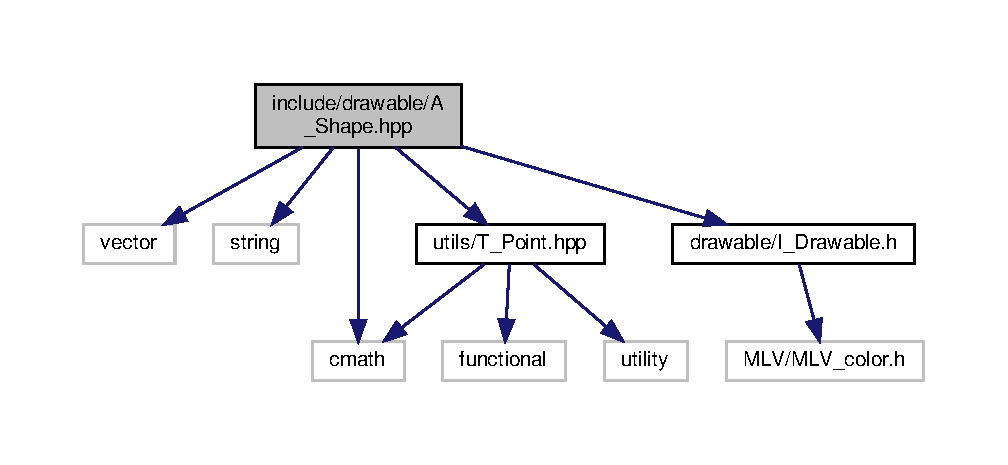
\includegraphics[width=350pt]{A__Shape_8hpp__incl}
\end{center}
\end{figure}
\subsection*{Classes}
\begin{DoxyCompactItemize}
\item 
class \hyperlink{classA__Shape}{A\+\_\+\+Shape}
\begin{DoxyCompactList}\small\item\em Abstract Class of every \hyperlink{classA__Shape}{A\+\_\+\+Shape}. \end{DoxyCompactList}\end{DoxyCompactItemize}

\hypertarget{C__Button_8hpp}{}\section{include/drawable/\+C\+\_\+\+Button.hpp File Reference}
\label{C__Button_8hpp}\index{include/drawable/\+C\+\_\+\+Button.\+hpp@{include/drawable/\+C\+\_\+\+Button.\+hpp}}


Every m\+Buttons of menu.  


{\ttfamily \#include $<$utility$>$}\newline
{\ttfamily \#include $<$utils/\+T\+\_\+\+Point.\+hpp$>$}\newline
{\ttfamily \#include $<$functional$>$}\newline
{\ttfamily \#include $<$M\+L\+V/\+M\+L\+V\+\_\+color.\+h$>$}\newline
Include dependency graph for C\+\_\+\+Button.\+hpp\+:\nopagebreak
\begin{figure}[H]
\begin{center}
\leavevmode
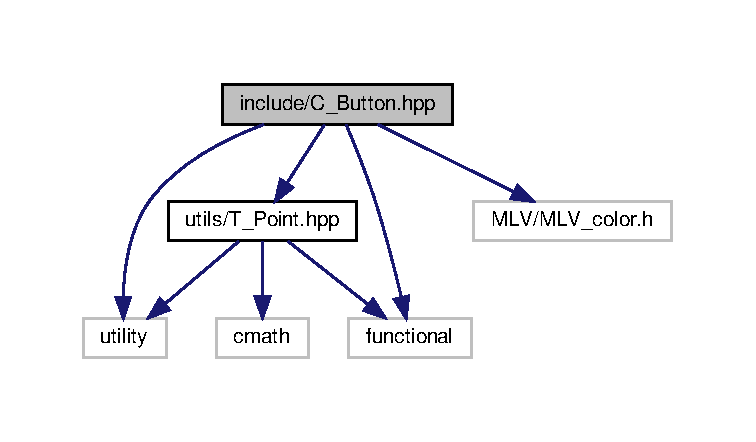
\includegraphics[width=350pt]{C__Button_8hpp__incl}
\end{center}
\end{figure}
This graph shows which files directly or indirectly include this file\+:\nopagebreak
\begin{figure}[H]
\begin{center}
\leavevmode
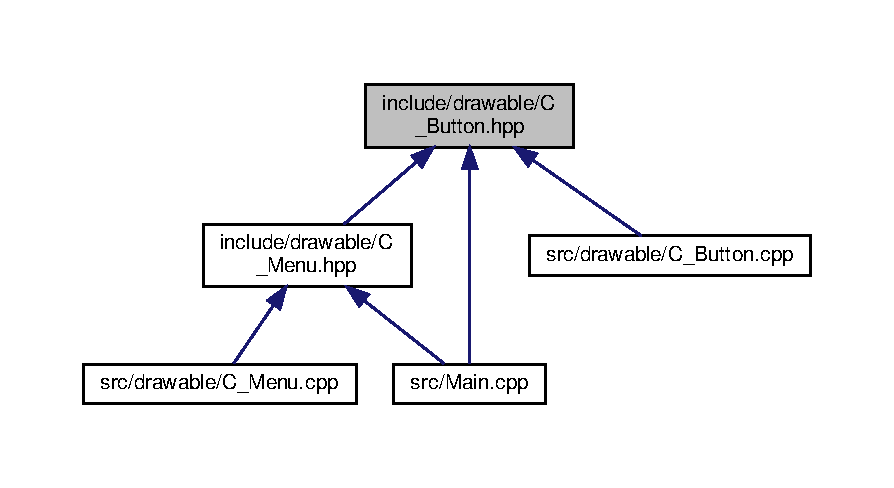
\includegraphics[width=350pt]{C__Button_8hpp__dep__incl}
\end{center}
\end{figure}
\subsection*{Classes}
\begin{DoxyCompactItemize}
\item 
class \hyperlink{classC__Button}{C\+\_\+\+Button}
\begin{DoxyCompactList}\small\item\em \hyperlink{classC__Button}{C\+\_\+\+Button} of the \hyperlink{classC__Menu}{C\+\_\+\+Menu}. \end{DoxyCompactList}\end{DoxyCompactItemize}


\subsection{Detailed Description}
Every m\+Buttons of menu. 

\begin{DoxyAuthor}{Author}
Jérémie LE B\+A\+S\+T\+A\+RD 
\end{DoxyAuthor}
\begin{DoxyVersion}{Version}
1.\+0 
\end{DoxyVersion}

\hypertarget{C__Menu_8hpp}{}\section{include/\+C\+\_\+\+Menu.hpp File Reference}
\label{C__Menu_8hpp}\index{include/\+C\+\_\+\+Menu.\+hpp@{include/\+C\+\_\+\+Menu.\+hpp}}
{\ttfamily \#include $<$drawable/\+C\+\_\+\+Button.\+hpp$>$}\newline
{\ttfamily \#include $<$vector$>$}\newline
Include dependency graph for C\+\_\+\+Menu.\+hpp\+:\nopagebreak
\begin{figure}[H]
\begin{center}
\leavevmode
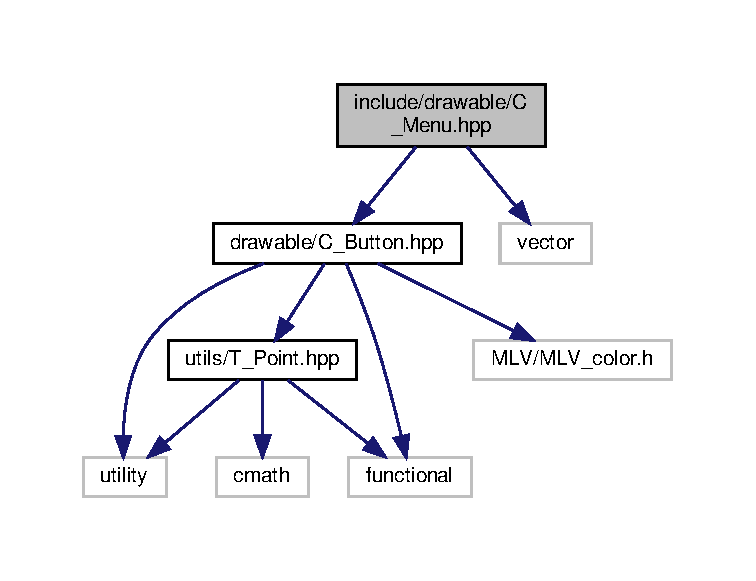
\includegraphics[width=350pt]{C__Menu_8hpp__incl}
\end{center}
\end{figure}
\subsection*{Classes}
\begin{DoxyCompactItemize}
\item 
class \hyperlink{classC__Menu}{C\+\_\+\+Menu}
\begin{DoxyCompactList}\small\item\em \hyperlink{classC__Menu}{C\+\_\+\+Menu} of the game. \end{DoxyCompactList}\end{DoxyCompactItemize}

\hypertarget{I__Drawable_8h}{}\section{include/drawable/\+I\+\_\+\+Drawable.h File Reference}
\label{I__Drawable_8h}\index{include/drawable/\+I\+\_\+\+Drawable.\+h@{include/drawable/\+I\+\_\+\+Drawable.\+h}}
{\ttfamily \#include $<$M\+L\+V/\+M\+L\+V\+\_\+color.\+h$>$}\newline
Include dependency graph for I\+\_\+\+Drawable.\+h\+:
\nopagebreak
\begin{figure}[H]
\begin{center}
\leavevmode
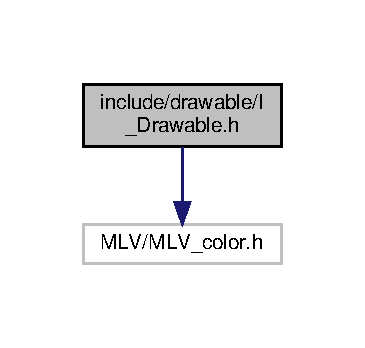
\includegraphics[width=175pt]{I__Drawable_8h__incl}
\end{center}
\end{figure}
This graph shows which files directly or indirectly include this file\+:\nopagebreak
\begin{figure}[H]
\begin{center}
\leavevmode
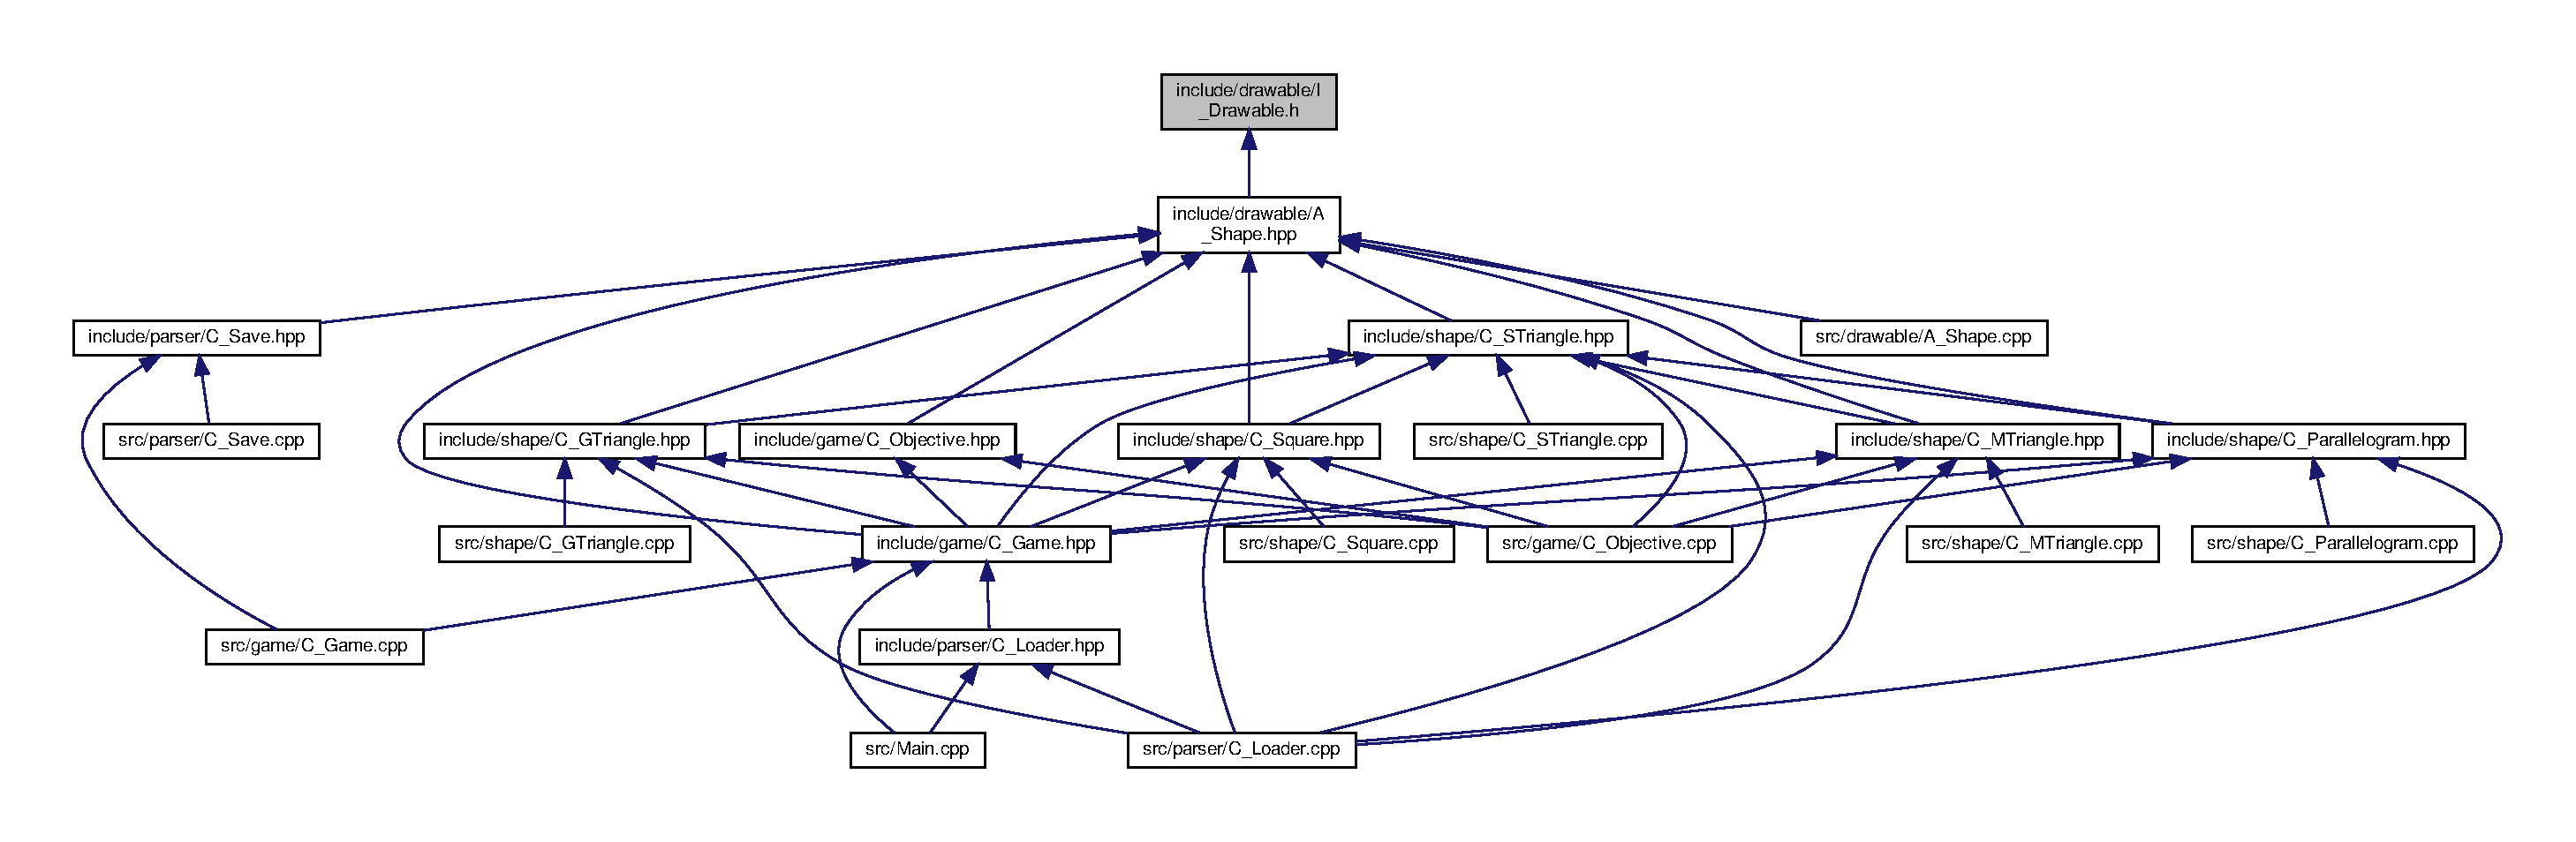
\includegraphics[width=350pt]{I__Drawable_8h__dep__incl}
\end{center}
\end{figure}
\subsection*{Classes}
\begin{DoxyCompactItemize}
\item 
class \hyperlink{classI__Drawable}{I\+\_\+\+Drawable}
\begin{DoxyCompactList}\small\item\em \hyperlink{classI__Drawable}{I\+\_\+\+Drawable} is everything to i\+Draw. \end{DoxyCompactList}\end{DoxyCompactItemize}

\hypertarget{C__Game_8hpp}{}\section{include/game/\+C\+\_\+\+Game.hpp File Reference}
\label{C__Game_8hpp}\index{include/game/\+C\+\_\+\+Game.\+hpp@{include/game/\+C\+\_\+\+Game.\+hpp}}


Main \hyperlink{classC__Game}{C\+\_\+\+Game} of the Tangram.  


{\ttfamily \#include $<$drawable/\+A\+\_\+\+Shape.\+hpp$>$}\newline
{\ttfamily \#include $<$utils/\+T\+\_\+\+Point.\+hpp$>$}\newline
{\ttfamily \#include $<$game/\+C\+\_\+\+Objective.\+hpp$>$}\newline
{\ttfamily \#include $<$shape/\+C\+\_\+\+S\+Triangle.\+hpp$>$}\newline
{\ttfamily \#include $<$shape/\+C\+\_\+\+M\+Triangle.\+hpp$>$}\newline
{\ttfamily \#include $<$shape/\+C\+\_\+\+G\+Triangle.\+hpp$>$}\newline
{\ttfamily \#include $<$shape/\+C\+\_\+\+Parallelogram.\+hpp$>$}\newline
{\ttfamily \#include $<$shape/\+C\+\_\+\+Square.\+hpp$>$}\newline
{\ttfamily \#include $<$M\+L\+V/\+M\+L\+V\+\_\+all.\+h$>$}\newline
{\ttfamily \#include $<$functional$>$}\newline
{\ttfamily \#include $<$unordered\+\_\+set$>$}\newline
{\ttfamily \#include $<$memory$>$}\newline
{\ttfamily \#include $<$iostream$>$}\newline
{\ttfamily \#include $<$unordered\+\_\+map$>$}\newline
Include dependency graph for C\+\_\+\+Game.\+hpp\+:\nopagebreak
\begin{figure}[H]
\begin{center}
\leavevmode
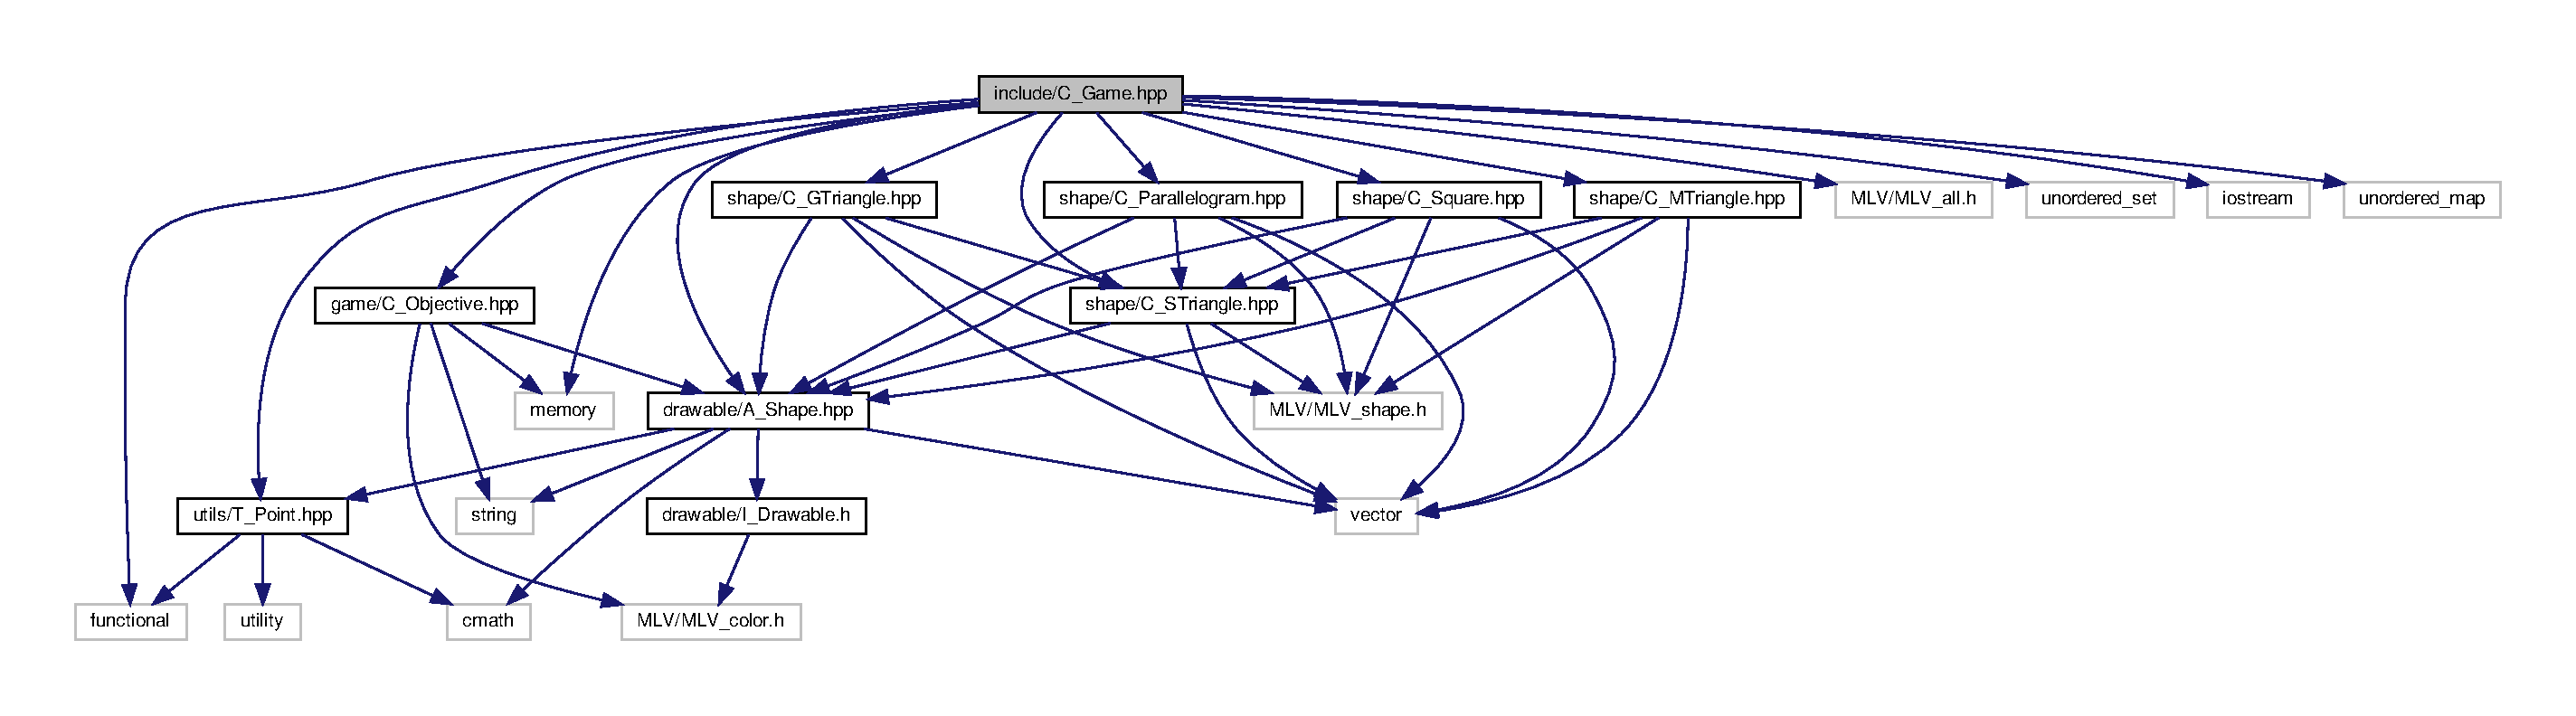
\includegraphics[width=350pt]{C__Game_8hpp__incl}
\end{center}
\end{figure}
This graph shows which files directly or indirectly include this file\+:\nopagebreak
\begin{figure}[H]
\begin{center}
\leavevmode
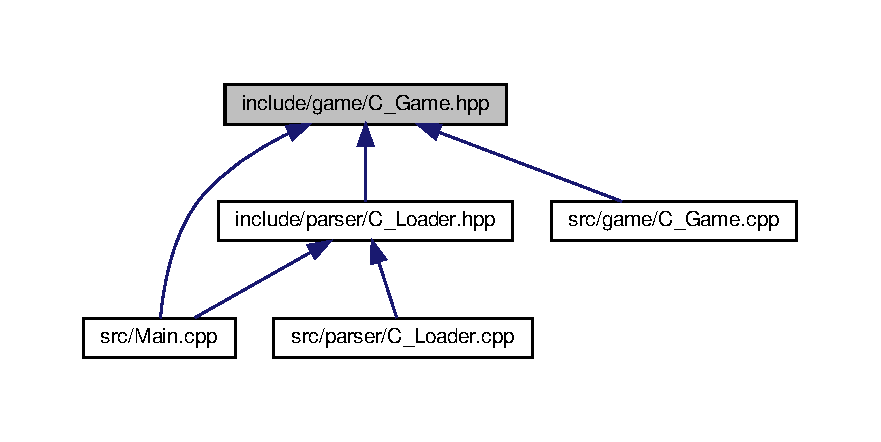
\includegraphics[width=350pt]{C__Game_8hpp__dep__incl}
\end{center}
\end{figure}
\subsection*{Classes}
\begin{DoxyCompactItemize}
\item 
class \hyperlink{classC__Game}{C\+\_\+\+Game}
\begin{DoxyCompactList}\small\item\em Class of the main \hyperlink{classC__Game}{C\+\_\+\+Game}. \end{DoxyCompactList}\end{DoxyCompactItemize}


\subsection{Detailed Description}
Main \hyperlink{classC__Game}{C\+\_\+\+Game} of the Tangram. 

\begin{DoxyAuthor}{Author}
Jérémie LE B\+A\+S\+T\+A\+RD 
\end{DoxyAuthor}
\begin{DoxyVersion}{Version}
1.\+0 
\end{DoxyVersion}

\hypertarget{C__Objective_8hpp}{}\section{include/game/\+C\+\_\+\+Objective.hpp File Reference}
\label{C__Objective_8hpp}\index{include/game/\+C\+\_\+\+Objective.\+hpp@{include/game/\+C\+\_\+\+Objective.\+hpp}}


\hyperlink{classC__Objective}{C\+\_\+\+Objective} of the Tangram\textquotesingle{}s board.  


{\ttfamily \#include $<$drawable/\+A\+\_\+\+Shape.\+hpp$>$}\newline
{\ttfamily \#include $<$string$>$}\newline
{\ttfamily \#include $<$memory$>$}\newline
{\ttfamily \#include $<$M\+L\+V/\+M\+L\+V\+\_\+color.\+h$>$}\newline
Include dependency graph for C\+\_\+\+Objective.\+hpp\+:\nopagebreak
\begin{figure}[H]
\begin{center}
\leavevmode
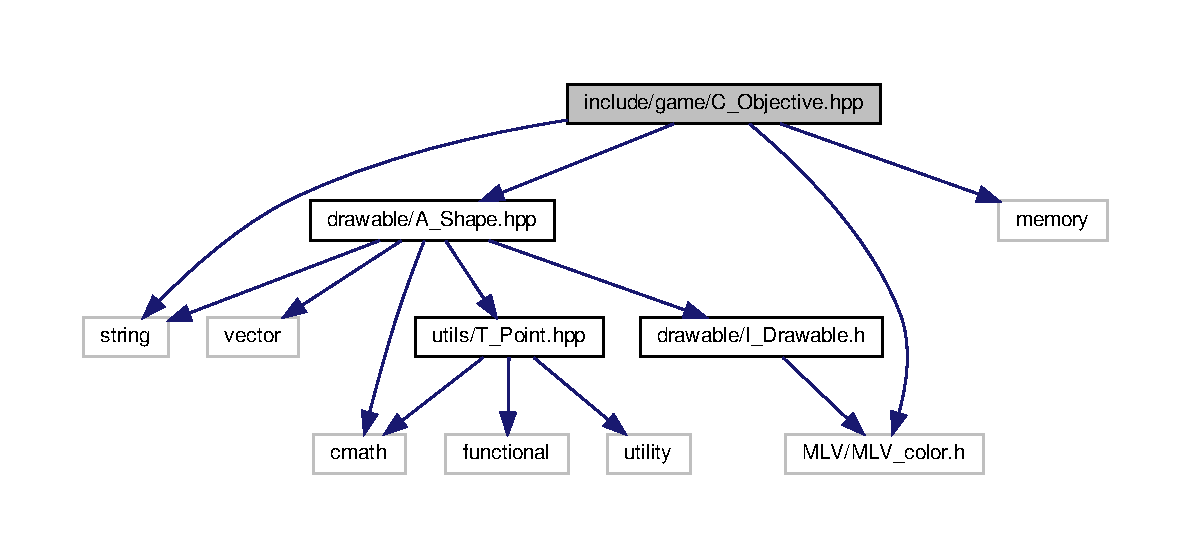
\includegraphics[width=350pt]{C__Objective_8hpp__incl}
\end{center}
\end{figure}
This graph shows which files directly or indirectly include this file\+:\nopagebreak
\begin{figure}[H]
\begin{center}
\leavevmode
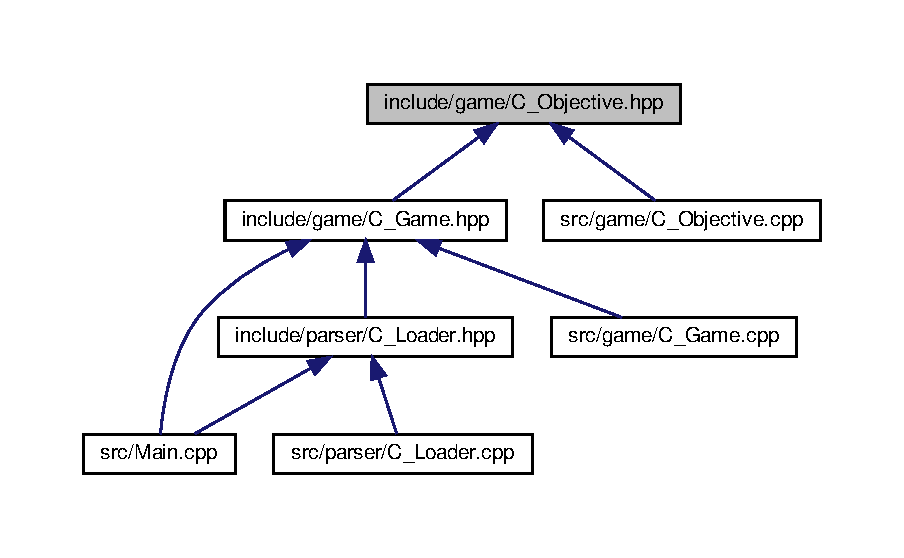
\includegraphics[width=350pt]{C__Objective_8hpp__dep__incl}
\end{center}
\end{figure}
\subsection*{Classes}
\begin{DoxyCompactItemize}
\item 
class \hyperlink{classC__Objective}{C\+\_\+\+Objective}
\begin{DoxyCompactList}\small\item\em Class of the board \hyperlink{classC__Objective}{C\+\_\+\+Objective}. \end{DoxyCompactList}\end{DoxyCompactItemize}


\subsection{Detailed Description}
\hyperlink{classC__Objective}{C\+\_\+\+Objective} of the Tangram\textquotesingle{}s board. 

\begin{DoxyAuthor}{Author}
Jérémie LE B\+A\+S\+T\+A\+RD 
\end{DoxyAuthor}
\begin{DoxyVersion}{Version}
1.\+0 
\end{DoxyVersion}

\hypertarget{C__Loader_8hpp}{}\section{include/parser/\+C\+\_\+\+Loader.hpp File Reference}
\label{C__Loader_8hpp}\index{include/parser/\+C\+\_\+\+Loader.\+hpp@{include/parser/\+C\+\_\+\+Loader.\+hpp}}


Load a board of Tangram.  


{\ttfamily \#include $<$game/\+C\+\_\+\+Game.\+hpp$>$}\newline
{\ttfamily \#include $<$filesystem$>$}\newline
{\ttfamily \#include $<$memory$>$}\newline
Include dependency graph for C\+\_\+\+Loader.\+hpp\+:
\nopagebreak
\begin{figure}[H]
\begin{center}
\leavevmode
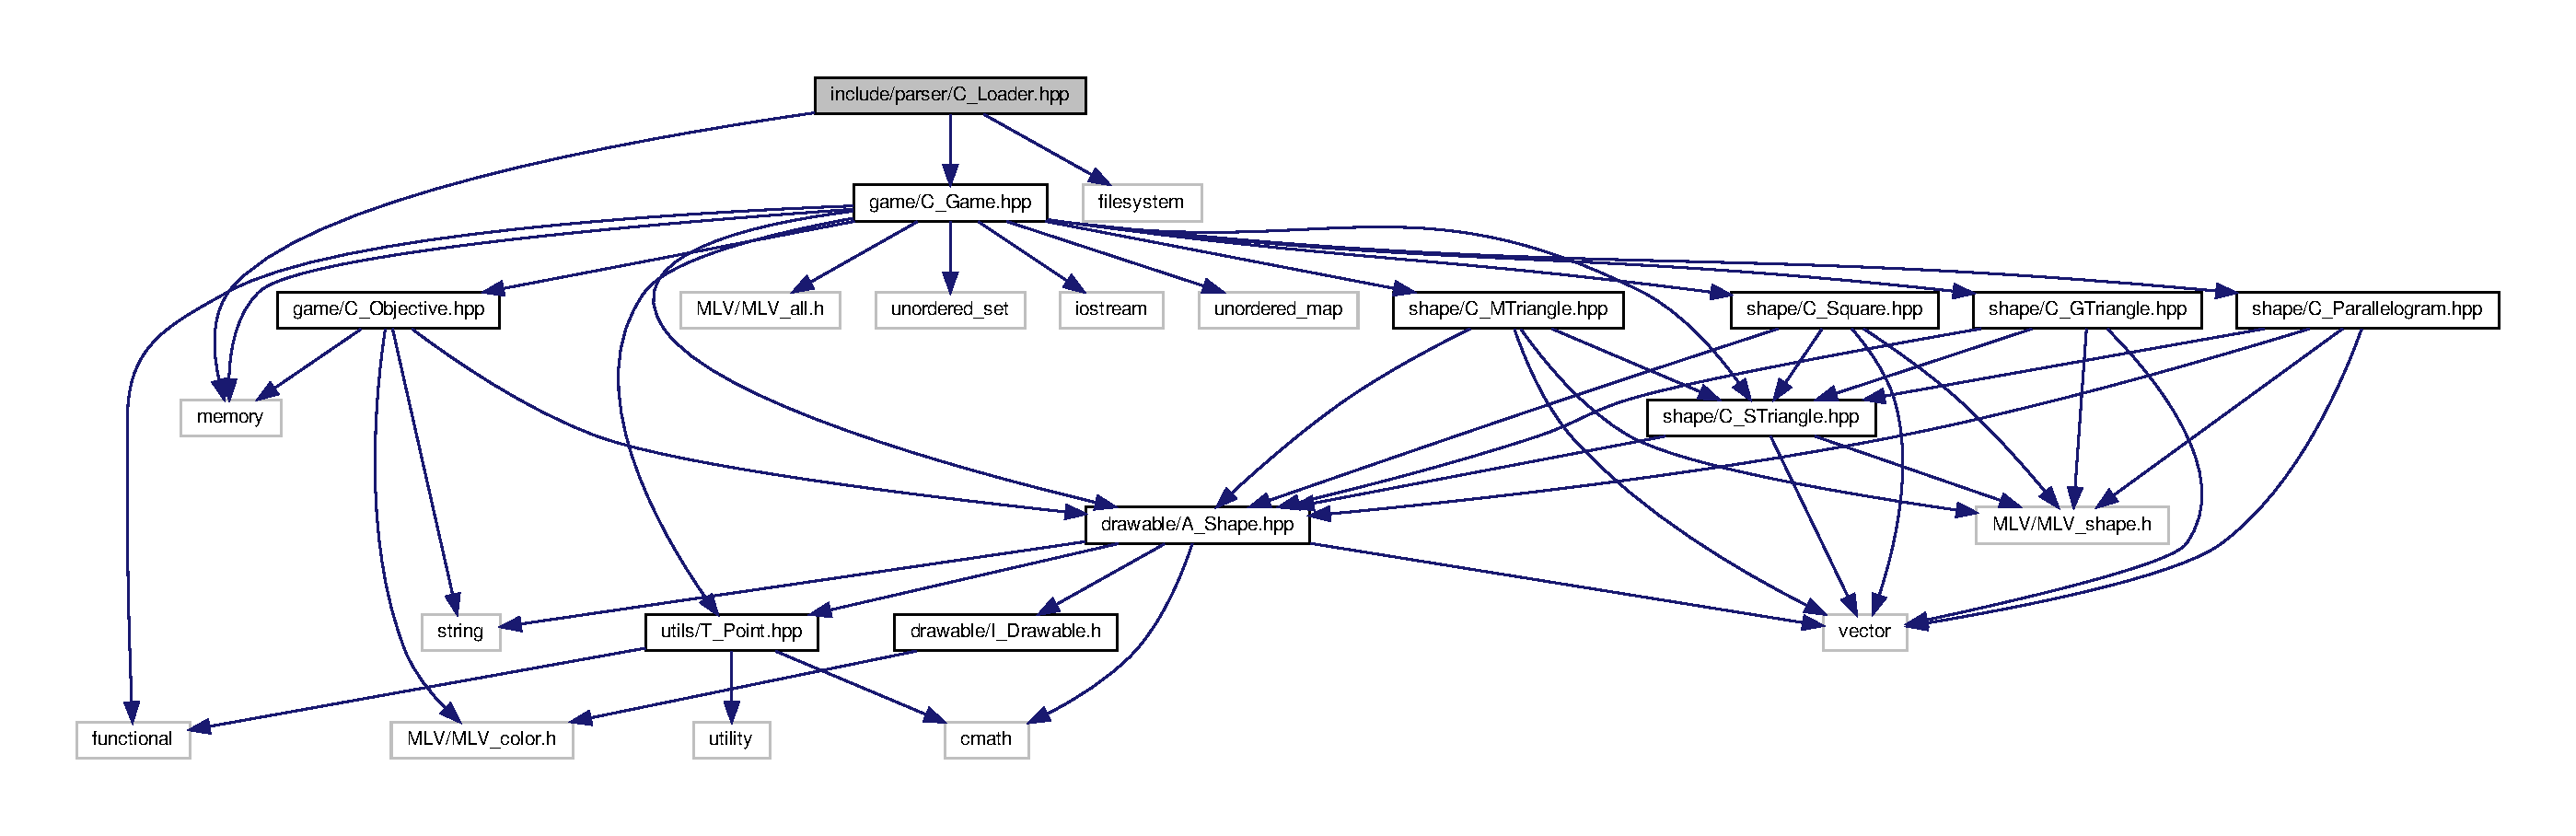
\includegraphics[width=350pt]{C__Loader_8hpp__incl}
\end{center}
\end{figure}
This graph shows which files directly or indirectly include this file\+:\nopagebreak
\begin{figure}[H]
\begin{center}
\leavevmode
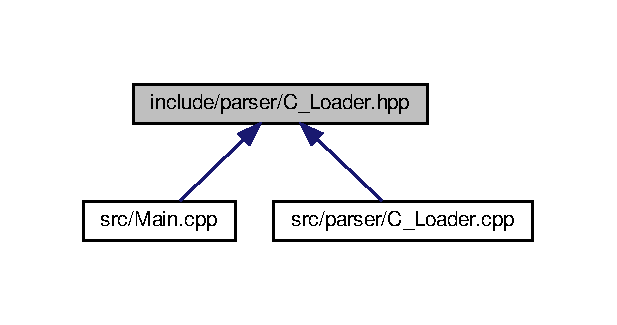
\includegraphics[width=296pt]{C__Loader_8hpp__dep__incl}
\end{center}
\end{figure}
\subsection*{Classes}
\begin{DoxyCompactItemize}
\item 
class \hyperlink{classC__Loader}{C\+\_\+\+Loader}
\begin{DoxyCompactList}\small\item\em Class of the main \hyperlink{classC__Loader}{C\+\_\+\+Loader}. \end{DoxyCompactList}\end{DoxyCompactItemize}


\subsection{Detailed Description}
Load a board of Tangram. 

\begin{DoxyAuthor}{Author}
Jérémie LE B\+A\+S\+T\+A\+RD 
\end{DoxyAuthor}
\begin{DoxyVersion}{Version}
1.\+0 
\end{DoxyVersion}

\hypertarget{C__Save_8hpp}{}\section{include/\+C\+\_\+\+Save.hpp File Reference}
\label{C__Save_8hpp}\index{include/\+C\+\_\+\+Save.\+hpp@{include/\+C\+\_\+\+Save.\+hpp}}
{\ttfamily \#include $<$string$>$}\newline
{\ttfamily \#include $<$filesystem$>$}\newline
{\ttfamily \#include $<$vector$>$}\newline
{\ttfamily \#include $<$fstream$>$}\newline
{\ttfamily \#include $<$drawable/\+A\+\_\+\+Shape.\+hpp$>$}\newline
Include dependency graph for C\+\_\+\+Save.\+hpp\+:\nopagebreak
\begin{figure}[H]
\begin{center}
\leavevmode
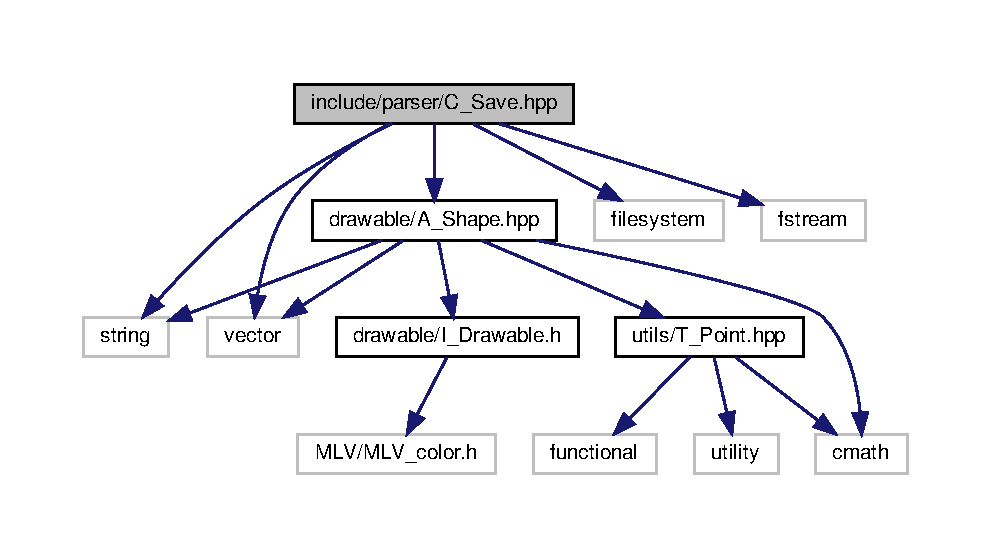
\includegraphics[width=350pt]{C__Save_8hpp__incl}
\end{center}
\end{figure}
\subsection*{Classes}
\begin{DoxyCompactItemize}
\item 
class \hyperlink{classC__Save}{C\+\_\+\+Save}
\begin{DoxyCompactList}\small\item\em Class of the main Saver. \end{DoxyCompactList}\end{DoxyCompactItemize}

\hypertarget{C__GTriangle_8hpp}{}\section{include/\+C\+\_\+\+G\+Triangle.hpp File Reference}
\label{C__GTriangle_8hpp}\index{include/\+C\+\_\+\+G\+Triangle.\+hpp@{include/\+C\+\_\+\+G\+Triangle.\+hpp}}
{\ttfamily \#include $<$vector$>$}\newline
{\ttfamily \#include $<$shape/\+C\+\_\+\+S\+Triangle.\+hpp$>$}\newline
{\ttfamily \#include $<$drawable/\+A\+\_\+\+Shape.\+hpp$>$}\newline
{\ttfamily \#include $<$M\+L\+V/\+M\+L\+V\+\_\+shape.\+h$>$}\newline
Include dependency graph for C\+\_\+\+G\+Triangle.\+hpp\+:\nopagebreak
\begin{figure}[H]
\begin{center}
\leavevmode
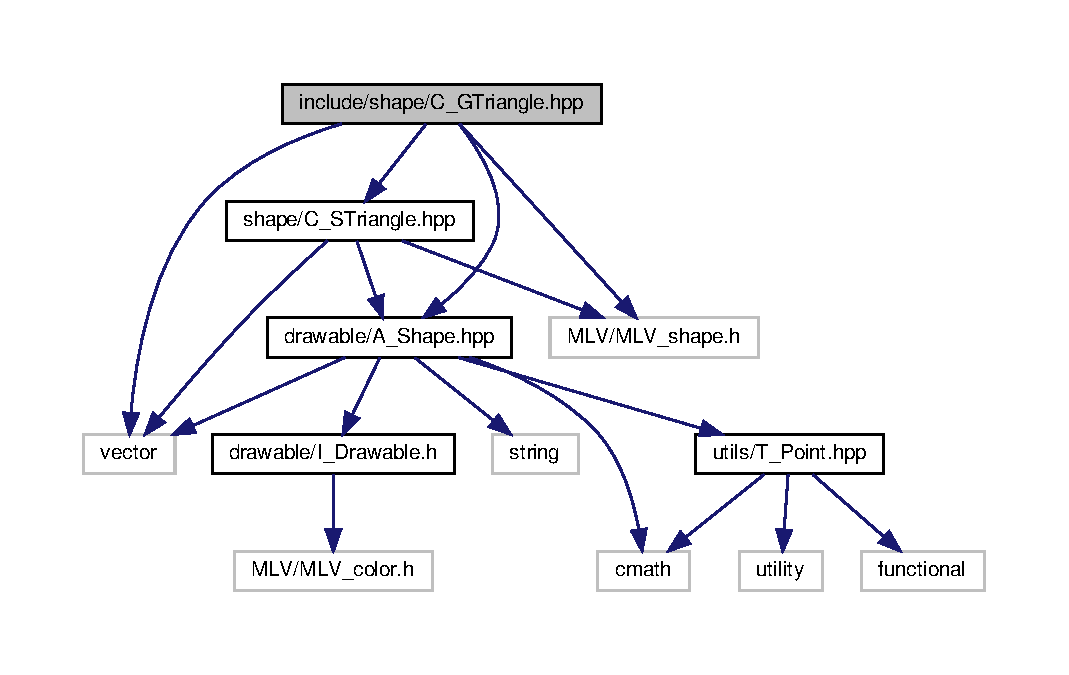
\includegraphics[width=350pt]{C__GTriangle_8hpp__incl}
\end{center}
\end{figure}
\subsection*{Classes}
\begin{DoxyCompactItemize}
\item 
class \hyperlink{classC__GTriangle}{C\+\_\+\+G\+Triangle}
\begin{DoxyCompactList}\small\item\em Class of the greatest m\+Triangles. \end{DoxyCompactList}\end{DoxyCompactItemize}

\hypertarget{C__MTriangle_8hpp}{}\section{include/shape/\+C\+\_\+\+M\+Triangle.hpp File Reference}
\label{C__MTriangle_8hpp}\index{include/shape/\+C\+\_\+\+M\+Triangle.\+hpp@{include/shape/\+C\+\_\+\+M\+Triangle.\+hpp}}


\hyperlink{classA__Shape}{A\+\_\+\+Shape} of Medium Triangle.  


{\ttfamily \#include $<$vector$>$}\newline
{\ttfamily \#include $<$shape/\+C\+\_\+\+S\+Triangle.\+hpp$>$}\newline
{\ttfamily \#include $<$drawable/\+A\+\_\+\+Shape.\+hpp$>$}\newline
{\ttfamily \#include $<$M\+L\+V/\+M\+L\+V\+\_\+shape.\+h$>$}\newline
Include dependency graph for C\+\_\+\+M\+Triangle.\+hpp\+:\nopagebreak
\begin{figure}[H]
\begin{center}
\leavevmode
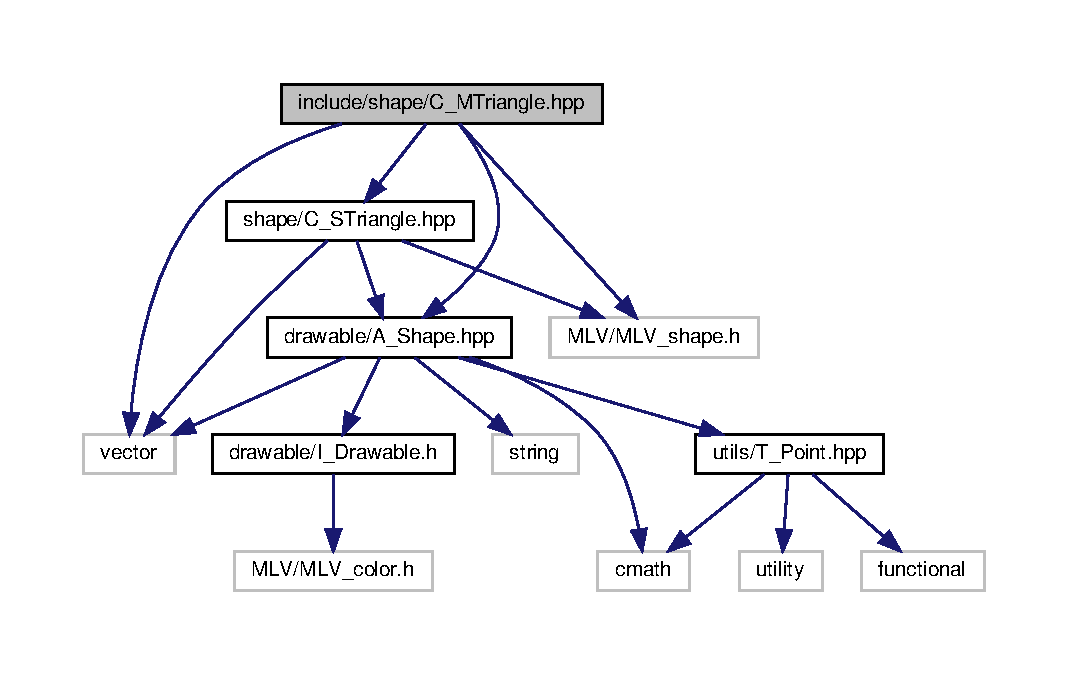
\includegraphics[width=350pt]{C__MTriangle_8hpp__incl}
\end{center}
\end{figure}
This graph shows which files directly or indirectly include this file\+:\nopagebreak
\begin{figure}[H]
\begin{center}
\leavevmode
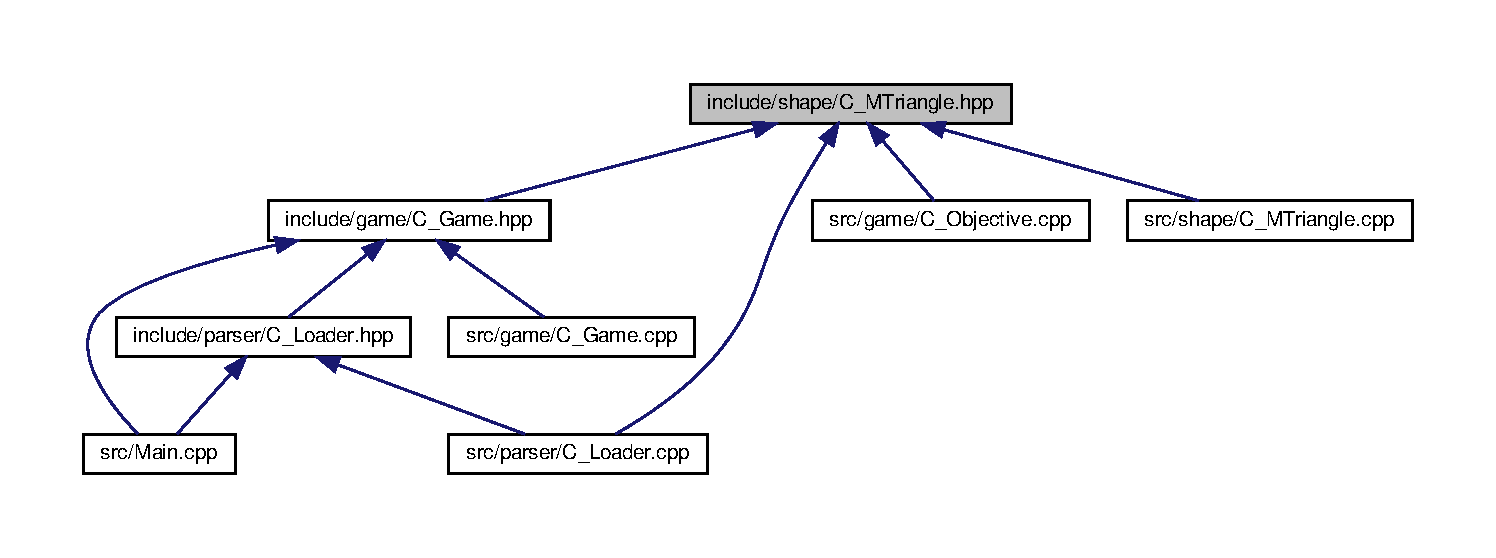
\includegraphics[width=350pt]{C__MTriangle_8hpp__dep__incl}
\end{center}
\end{figure}
\subsection*{Classes}
\begin{DoxyCompactItemize}
\item 
class \hyperlink{classC__MTriangle}{C\+\_\+\+M\+Triangle}
\begin{DoxyCompactList}\small\item\em Class of the medium \hyperlink{classC__MTriangle}{C\+\_\+\+M\+Triangle}. \end{DoxyCompactList}\end{DoxyCompactItemize}


\subsection{Detailed Description}
\hyperlink{classA__Shape}{A\+\_\+\+Shape} of Medium Triangle. 

\begin{DoxyAuthor}{Author}
Jérémie LE B\+A\+S\+T\+A\+RD 
\end{DoxyAuthor}
\begin{DoxyVersion}{Version}
1.\+0 
\end{DoxyVersion}

\hypertarget{C__Parallelogram_8hpp}{}\section{include/\+C\+\_\+\+Parallelogram.hpp File Reference}
\label{C__Parallelogram_8hpp}\index{include/\+C\+\_\+\+Parallelogram.\+hpp@{include/\+C\+\_\+\+Parallelogram.\+hpp}}
{\ttfamily \#include $<$vector$>$}\newline
{\ttfamily \#include $<$shape/\+C\+\_\+\+S\+Triangle.\+hpp$>$}\newline
{\ttfamily \#include $<$drawable/\+A\+\_\+\+Shape.\+hpp$>$}\newline
{\ttfamily \#include $<$M\+L\+V/\+M\+L\+V\+\_\+shape.\+h$>$}\newline
Include dependency graph for C\+\_\+\+Parallelogram.\+hpp\+:\nopagebreak
\begin{figure}[H]
\begin{center}
\leavevmode
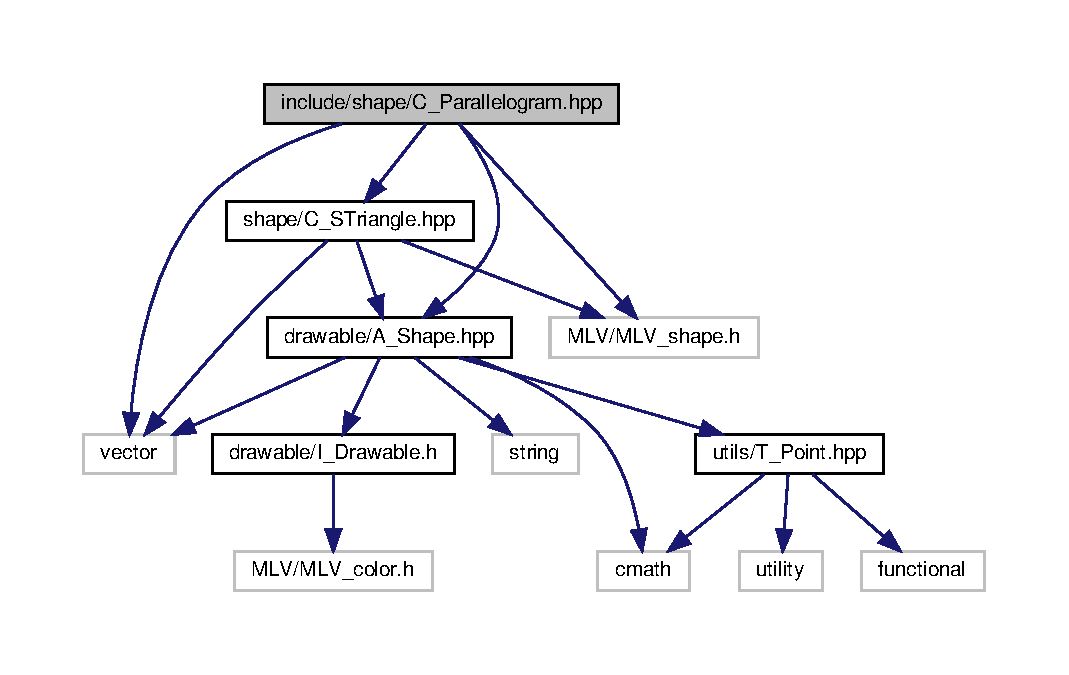
\includegraphics[width=350pt]{C__Parallelogram_8hpp__incl}
\end{center}
\end{figure}
\subsection*{Classes}
\begin{DoxyCompactItemize}
\item 
class \hyperlink{classC__Parallelogram}{C\+\_\+\+Parallelogram}
\begin{DoxyCompactList}\small\item\em Class of the parallelogram. \end{DoxyCompactList}\end{DoxyCompactItemize}

\hypertarget{C__Square_8hpp}{}\section{include/shape/\+C\+\_\+\+Square.hpp File Reference}
\label{C__Square_8hpp}\index{include/shape/\+C\+\_\+\+Square.\+hpp@{include/shape/\+C\+\_\+\+Square.\+hpp}}


\hyperlink{classA__Shape}{A\+\_\+\+Shape} of \hyperlink{classC__Square}{C\+\_\+\+Square}.  


{\ttfamily \#include $<$vector$>$}\newline
{\ttfamily \#include $<$shape/\+C\+\_\+\+S\+Triangle.\+hpp$>$}\newline
{\ttfamily \#include $<$drawable/\+A\+\_\+\+Shape.\+hpp$>$}\newline
{\ttfamily \#include $<$M\+L\+V/\+M\+L\+V\+\_\+shape.\+h$>$}\newline
Include dependency graph for C\+\_\+\+Square.\+hpp\+:\nopagebreak
\begin{figure}[H]
\begin{center}
\leavevmode
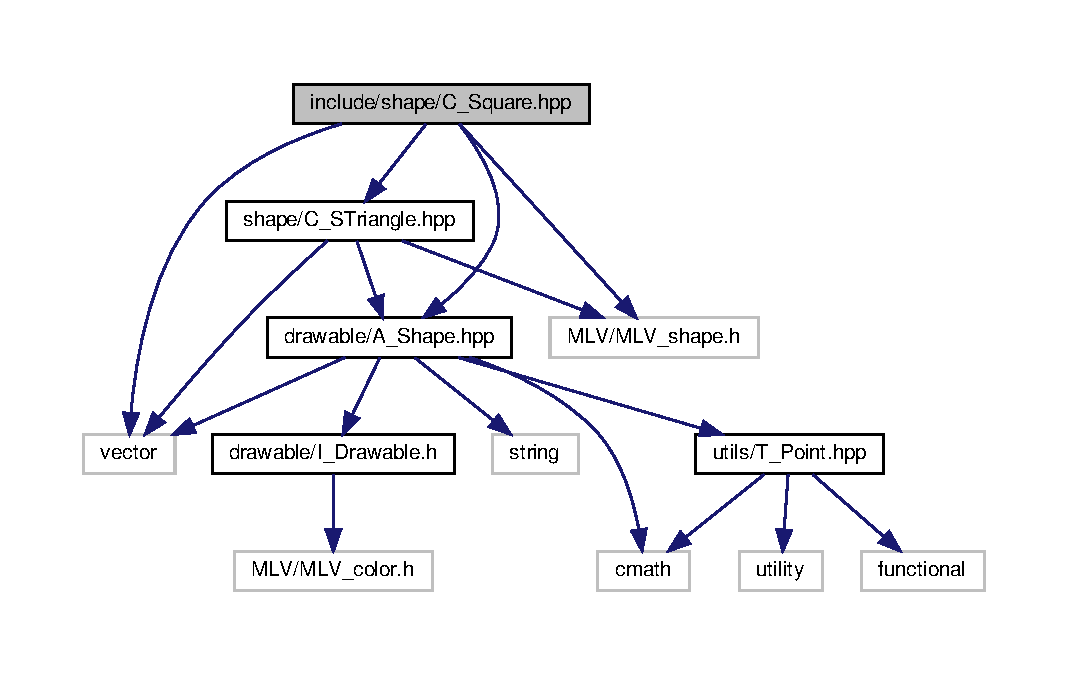
\includegraphics[width=350pt]{C__Square_8hpp__incl}
\end{center}
\end{figure}
This graph shows which files directly or indirectly include this file\+:\nopagebreak
\begin{figure}[H]
\begin{center}
\leavevmode
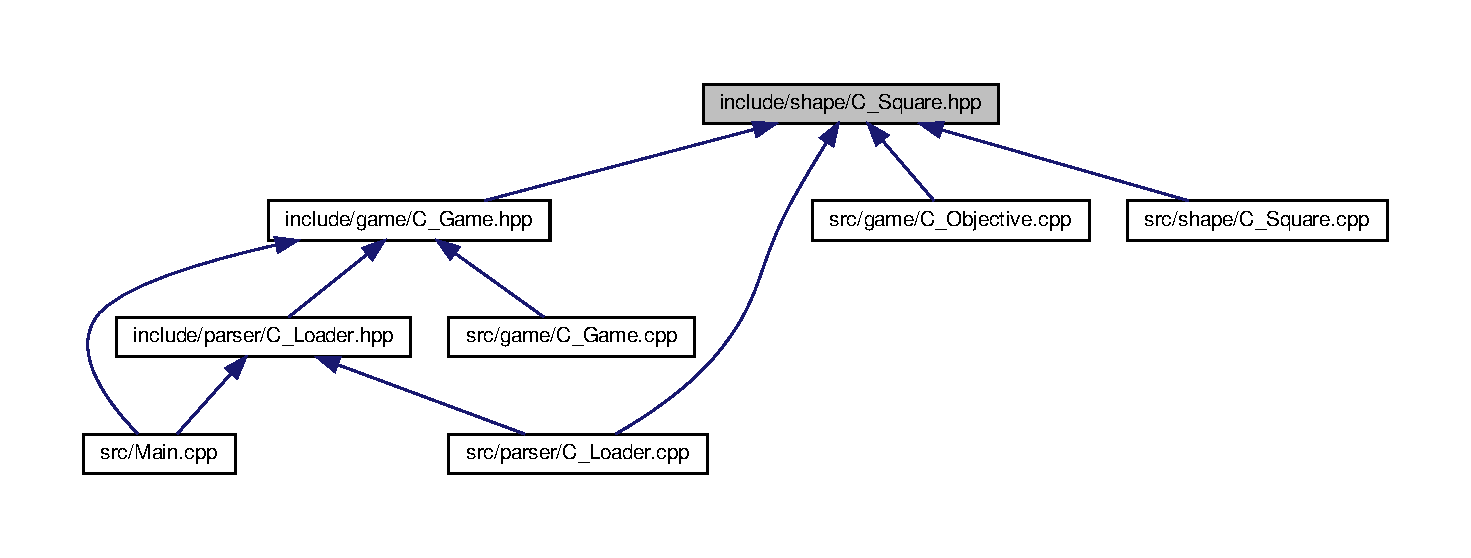
\includegraphics[width=350pt]{C__Square_8hpp__dep__incl}
\end{center}
\end{figure}
\subsection*{Classes}
\begin{DoxyCompactItemize}
\item 
class \hyperlink{classC__Square}{C\+\_\+\+Square}
\begin{DoxyCompactList}\small\item\em Class of the square. \end{DoxyCompactList}\end{DoxyCompactItemize}


\subsection{Detailed Description}
\hyperlink{classA__Shape}{A\+\_\+\+Shape} of \hyperlink{classC__Square}{C\+\_\+\+Square}. 

\begin{DoxyAuthor}{Author}
Jérémie LE B\+A\+S\+T\+A\+RD 
\end{DoxyAuthor}
\begin{DoxyVersion}{Version}
1.\+0 
\end{DoxyVersion}

\hypertarget{C__STriangle_8hpp}{}\section{include/shape/\+C\+\_\+\+S\+Triangle.hpp File Reference}
\label{C__STriangle_8hpp}\index{include/shape/\+C\+\_\+\+S\+Triangle.\+hpp@{include/shape/\+C\+\_\+\+S\+Triangle.\+hpp}}


\hyperlink{classA__Shape}{A\+\_\+\+Shape} of Small Triangle.  


{\ttfamily \#include $<$vector$>$}\newline
{\ttfamily \#include $<$drawable/\+A\+\_\+\+Shape.\+hpp$>$}\newline
{\ttfamily \#include $<$M\+L\+V/\+M\+L\+V\+\_\+shape.\+h$>$}\newline
Include dependency graph for C\+\_\+\+S\+Triangle.\+hpp\+:\nopagebreak
\begin{figure}[H]
\begin{center}
\leavevmode
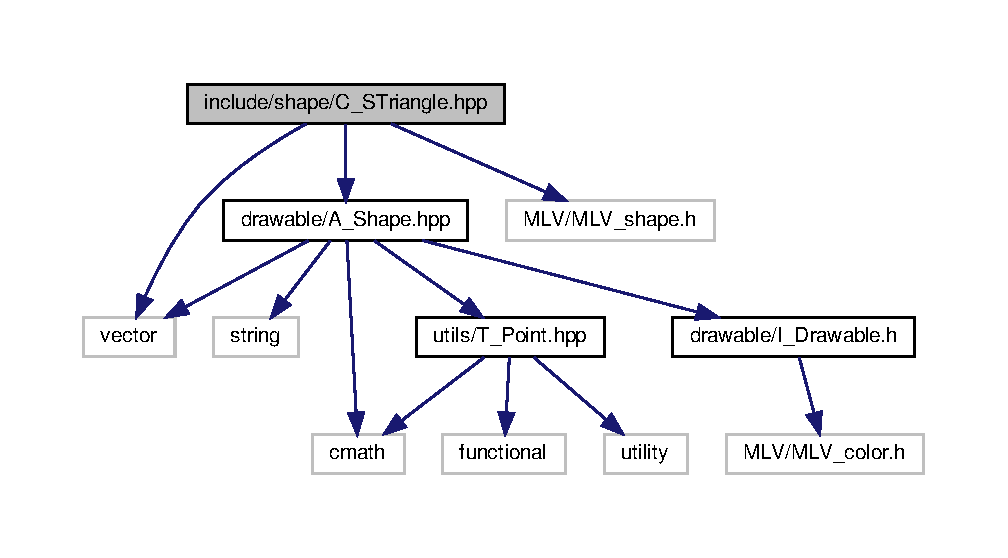
\includegraphics[width=350pt]{C__STriangle_8hpp__incl}
\end{center}
\end{figure}
This graph shows which files directly or indirectly include this file\+:\nopagebreak
\begin{figure}[H]
\begin{center}
\leavevmode
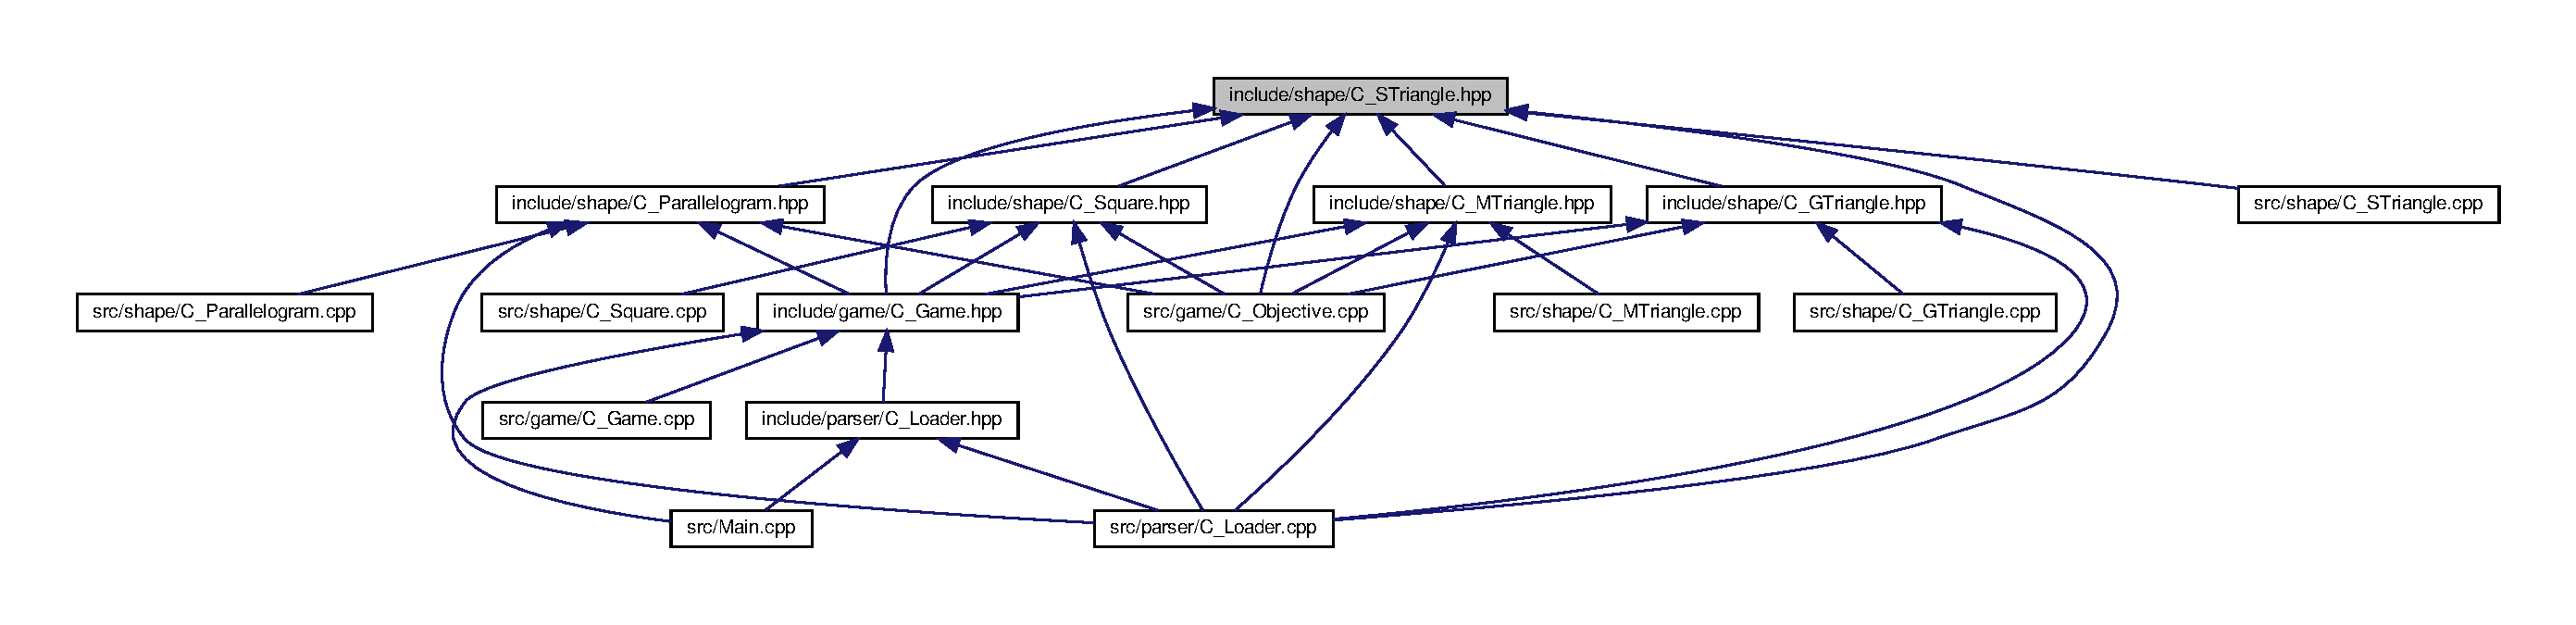
\includegraphics[width=350pt]{C__STriangle_8hpp__dep__incl}
\end{center}
\end{figure}
\subsection*{Classes}
\begin{DoxyCompactItemize}
\item 
class \hyperlink{classC__STriangle}{C\+\_\+\+S\+Triangle}
\begin{DoxyCompactList}\small\item\em Class of the small \hyperlink{classC__STriangle}{C\+\_\+\+S\+Triangle}. \end{DoxyCompactList}\end{DoxyCompactItemize}


\subsection{Detailed Description}
\hyperlink{classA__Shape}{A\+\_\+\+Shape} of Small Triangle. 

\begin{DoxyAuthor}{Author}
Jérémie LE B\+A\+S\+T\+A\+RD 
\end{DoxyAuthor}
\begin{DoxyVersion}{Version}
1.\+0 
\end{DoxyVersion}

\hypertarget{T__Point_8hpp}{}\section{include/\+T\+\_\+\+Point.hpp File Reference}
\label{T__Point_8hpp}\index{include/\+T\+\_\+\+Point.\+hpp@{include/\+T\+\_\+\+Point.\+hpp}}
{\ttfamily \#include $<$functional$>$}\newline
{\ttfamily \#include $<$utility$>$}\newline
{\ttfamily \#include $<$cmath$>$}\newline
Include dependency graph for T\+\_\+\+Point.\+hpp\+:\nopagebreak
\begin{figure}[H]
\begin{center}
\leavevmode
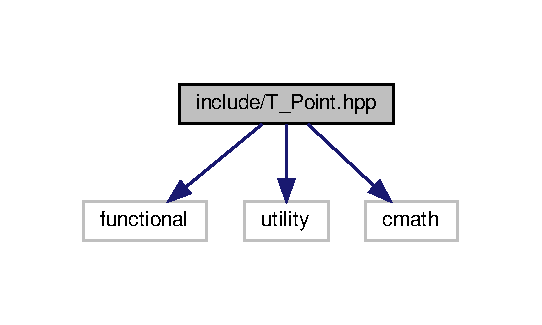
\includegraphics[width=260pt]{T__Point_8hpp__incl}
\end{center}
\end{figure}
\subsection*{Classes}
\begin{DoxyCompactItemize}
\item 
class \hyperlink{classT__Point}{T\+\_\+\+Point$<$ T $>$}
\begin{DoxyCompactList}\small\item\em Class of a \hyperlink{classT__Point}{T\+\_\+\+Point}. \end{DoxyCompactList}\item 
struct \hyperlink{structT__Point_1_1hash__point}{T\+\_\+\+Point$<$ T $>$\+::hash\+\_\+point}
\end{DoxyCompactItemize}

\hypertarget{README_8md}{}\section{R\+E\+A\+D\+M\+E.\+md File Reference}
\label{README_8md}\index{R\+E\+A\+D\+M\+E.\+md@{R\+E\+A\+D\+M\+E.\+md}}

\hypertarget{A__Shape_8cpp}{}\section{src/drawable/\+A\+\_\+\+Shape.cpp File Reference}
\label{A__Shape_8cpp}\index{src/drawable/\+A\+\_\+\+Shape.\+cpp@{src/drawable/\+A\+\_\+\+Shape.\+cpp}}
{\ttfamily \#include $<$iostream$>$}\newline
{\ttfamily \#include $<$cmath$>$}\newline
{\ttfamily \#include $<$drawable/\+A\+\_\+\+Shape.\+hpp$>$}\newline
Include dependency graph for A\+\_\+\+Shape.\+cpp\+:\nopagebreak
\begin{figure}[H]
\begin{center}
\leavevmode
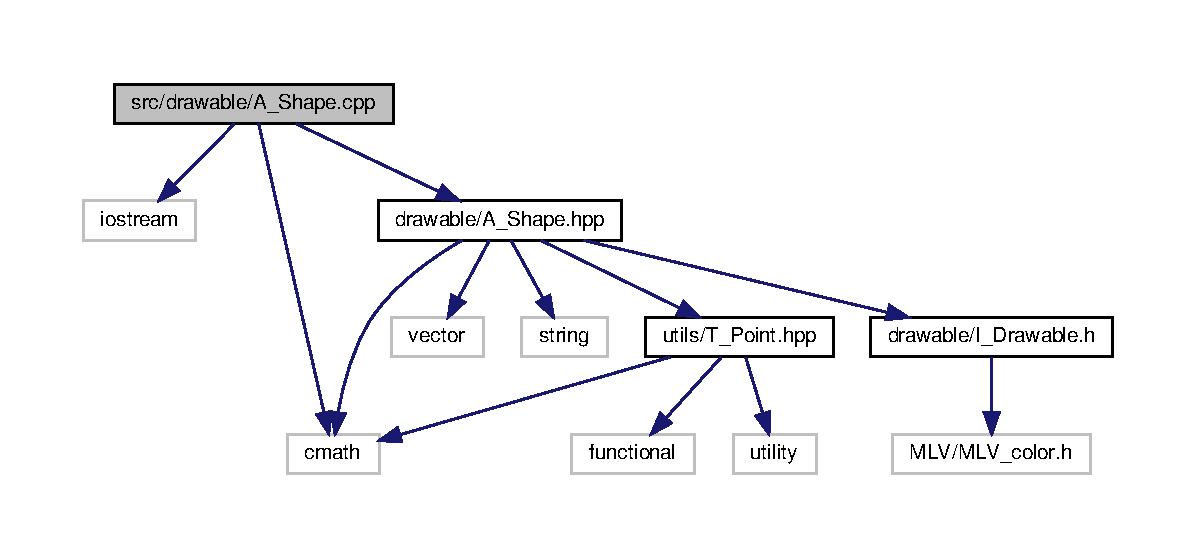
\includegraphics[width=350pt]{A__Shape_8cpp__incl}
\end{center}
\end{figure}

\hypertarget{C__Button_8cpp}{}\section{src/drawable/\+C\+\_\+\+Button.cpp File Reference}
\label{C__Button_8cpp}\index{src/drawable/\+C\+\_\+\+Button.\+cpp@{src/drawable/\+C\+\_\+\+Button.\+cpp}}
{\ttfamily \#include $<$string$>$}\newline
{\ttfamily \#include $<$drawable/\+C\+\_\+\+Button.\+hpp$>$}\newline
{\ttfamily \#include $<$utility$>$}\newline
{\ttfamily \#include $<$M\+L\+V/\+M\+L\+V\+\_\+color.\+h$>$}\newline
{\ttfamily \#include $<$M\+L\+V/\+M\+L\+V\+\_\+text.\+h$>$}\newline
Include dependency graph for C\+\_\+\+Button.\+cpp\+:\nopagebreak
\begin{figure}[H]
\begin{center}
\leavevmode
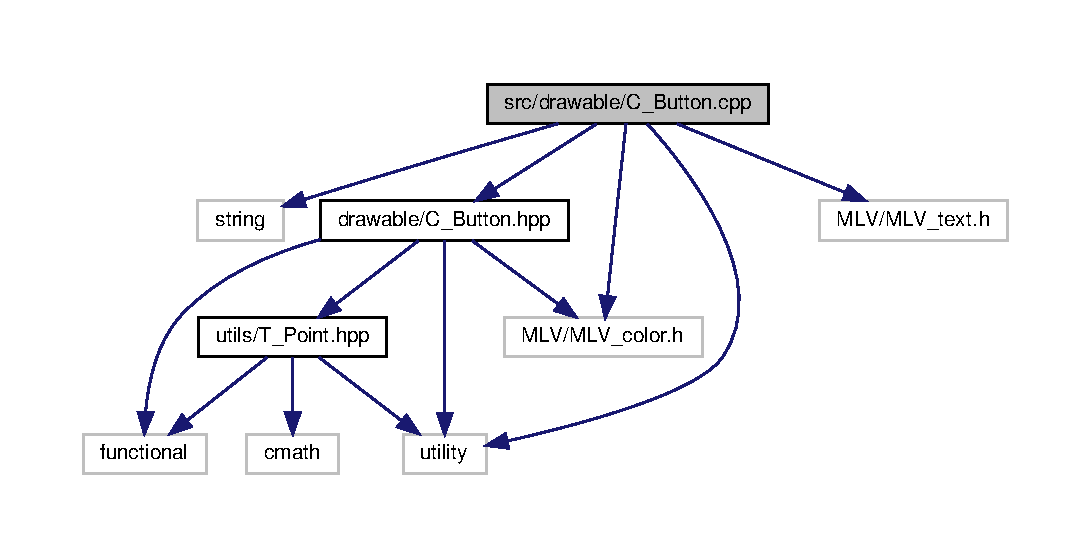
\includegraphics[width=350pt]{C__Button_8cpp__incl}
\end{center}
\end{figure}

\hypertarget{C__Menu_8cpp}{}\section{src/drawable/\+C\+\_\+\+Menu.cpp File Reference}
\label{C__Menu_8cpp}\index{src/drawable/\+C\+\_\+\+Menu.\+cpp@{src/drawable/\+C\+\_\+\+Menu.\+cpp}}
{\ttfamily \#include $<$drawable/\+C\+\_\+\+Menu.\+hpp$>$}\newline
{\ttfamily \#include $<$utils/\+T\+\_\+\+Point.\+hpp$>$}\newline
{\ttfamily \#include $<$M\+L\+V/\+M\+L\+V\+\_\+all.\+h$>$}\newline
Include dependency graph for C\+\_\+\+Menu.\+cpp\+:
\nopagebreak
\begin{figure}[H]
\begin{center}
\leavevmode
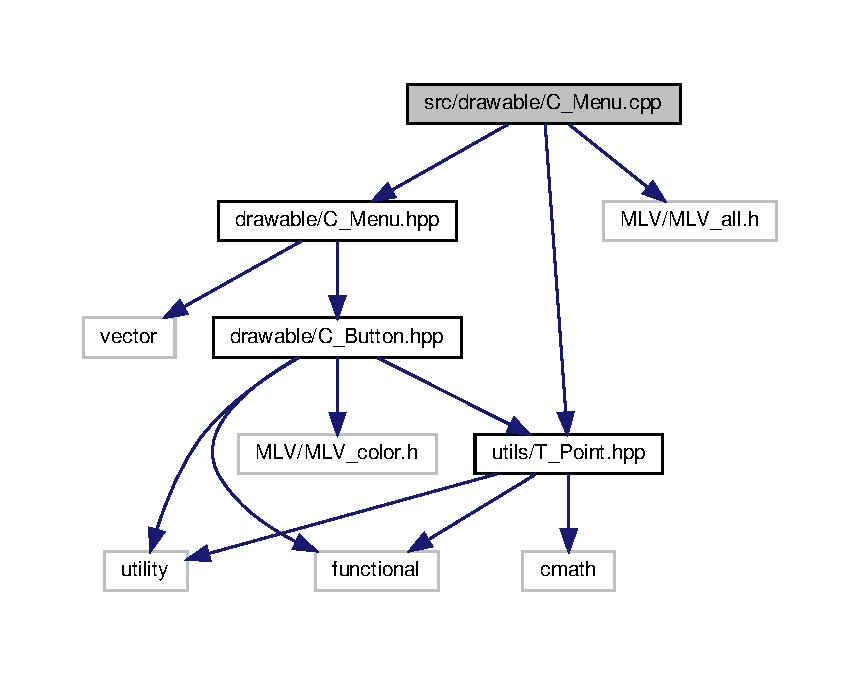
\includegraphics[width=350pt]{C__Menu_8cpp__incl}
\end{center}
\end{figure}

\hypertarget{I__Drawable_8cpp}{}\section{src/drawable/\+I\+\_\+\+Drawable.cpp File Reference}
\label{I__Drawable_8cpp}\index{src/drawable/\+I\+\_\+\+Drawable.\+cpp@{src/drawable/\+I\+\_\+\+Drawable.\+cpp}}

\hypertarget{C__Game_8cpp}{}\section{src/game/\+C\+\_\+\+Game.cpp File Reference}
\label{C__Game_8cpp}\index{src/game/\+C\+\_\+\+Game.\+cpp@{src/game/\+C\+\_\+\+Game.\+cpp}}
{\ttfamily \#include $<$iomanip$>$}\newline
{\ttfamily \#include $<$utility$>$}\newline
{\ttfamily \#include $<$game/\+C\+\_\+\+Game.\+hpp$>$}\newline
{\ttfamily \#include $<$parser/\+C\+\_\+\+Save.\+hpp$>$}\newline
Include dependency graph for C\+\_\+\+Game.\+cpp\+:\nopagebreak
\begin{figure}[H]
\begin{center}
\leavevmode
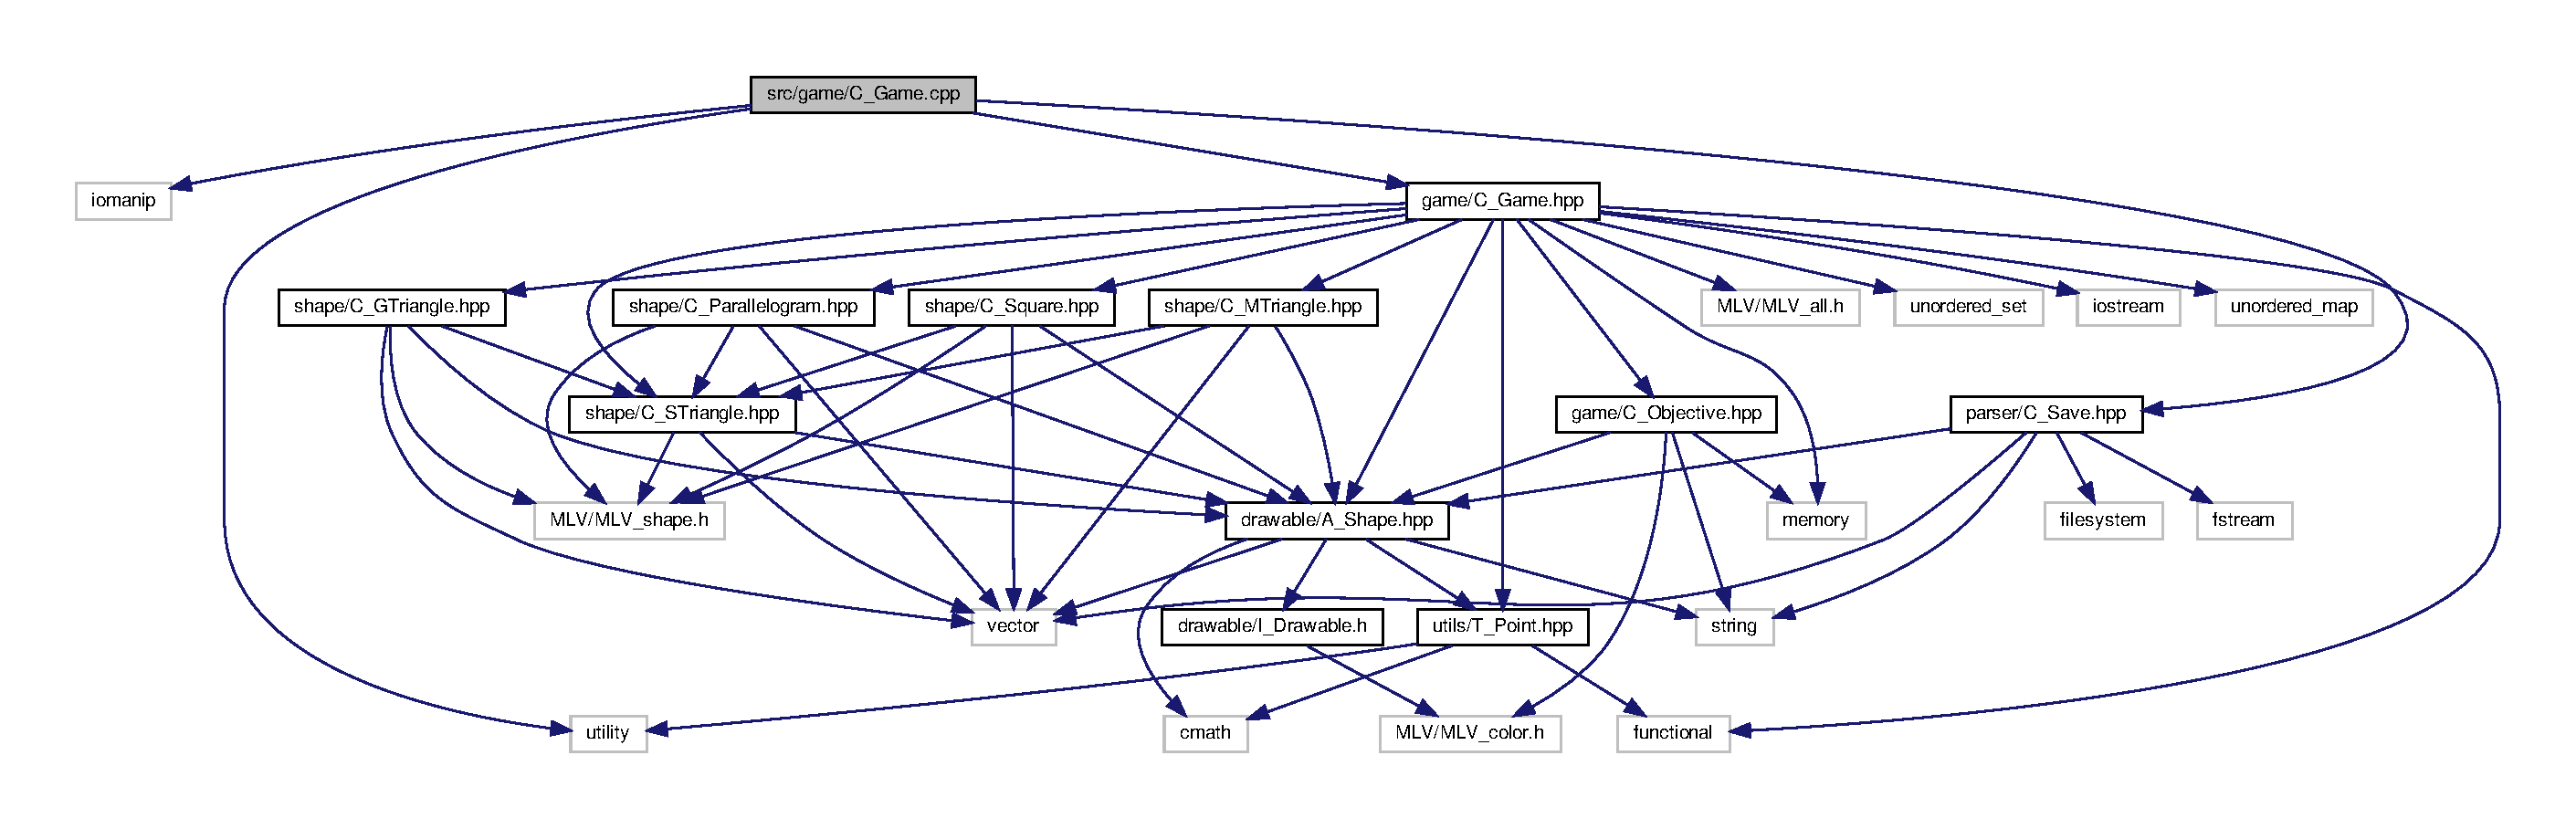
\includegraphics[width=350pt]{C__Game_8cpp__incl}
\end{center}
\end{figure}

\hypertarget{C__Objective_8cpp}{}\section{src/game/\+C\+\_\+\+Objective.cpp File Reference}
\label{C__Objective_8cpp}\index{src/game/\+C\+\_\+\+Objective.\+cpp@{src/game/\+C\+\_\+\+Objective.\+cpp}}
{\ttfamily \#include $<$game/\+C\+\_\+\+Objective.\+hpp$>$}\newline
{\ttfamily \#include $<$shape/\+C\+\_\+\+S\+Triangle.\+hpp$>$}\newline
{\ttfamily \#include $<$shape/\+C\+\_\+\+M\+Triangle.\+hpp$>$}\newline
{\ttfamily \#include $<$shape/\+C\+\_\+\+G\+Triangle.\+hpp$>$}\newline
{\ttfamily \#include $<$shape/\+C\+\_\+\+Parallelogram.\+hpp$>$}\newline
{\ttfamily \#include $<$shape/\+C\+\_\+\+Square.\+hpp$>$}\newline
{\ttfamily \#include $<$algorithm$>$}\newline
{\ttfamily \#include $<$iostream$>$}\newline
{\ttfamily \#include $<$memory$>$}\newline
{\ttfamily \#include $<$bits/unordered\+\_\+set.\+h$>$}\newline
Include dependency graph for C\+\_\+\+Objective.\+cpp\+:
\nopagebreak
\begin{figure}[H]
\begin{center}
\leavevmode
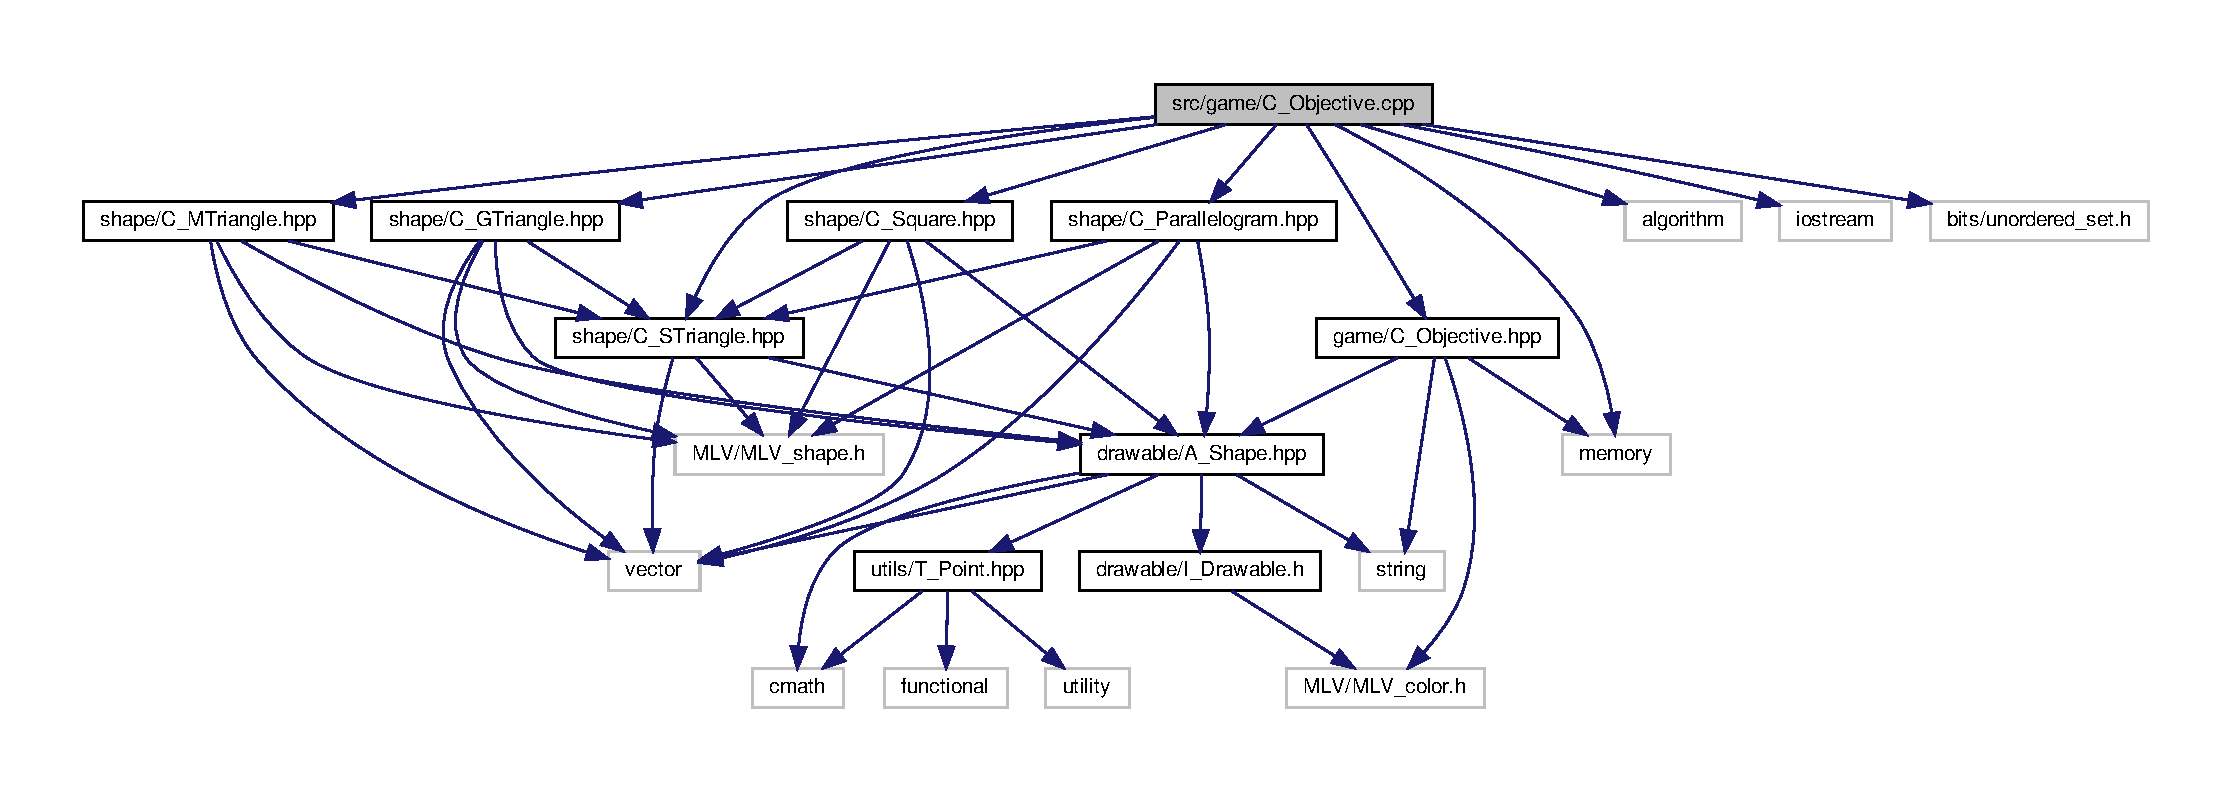
\includegraphics[width=350pt]{C__Objective_8cpp__incl}
\end{center}
\end{figure}

\hypertarget{Main_8cpp}{}\section{src/\+Main.cpp File Reference}
\label{Main_8cpp}\index{src/\+Main.\+cpp@{src/\+Main.\+cpp}}
{\ttfamily \#include $<$parser/\+C\+\_\+\+Loader.\+hpp$>$}\newline
{\ttfamily \#include $<$drawable/\+C\+\_\+\+Menu.\+hpp$>$}\newline
{\ttfamily \#include $<$drawable/\+C\+\_\+\+Button.\+hpp$>$}\newline
{\ttfamily \#include $<$M\+L\+V/\+M\+L\+V\+\_\+all.\+h$>$}\newline
{\ttfamily \#include $<$game/\+C\+\_\+\+Game.\+hpp$>$}\newline
{\ttfamily \#include $<$filesystem$>$}\newline
Include dependency graph for Main.\+cpp\+:
\nopagebreak
\begin{figure}[H]
\begin{center}
\leavevmode
\includegraphics[width=350pt]{Main_8cpp__incl}
\end{center}
\end{figure}
\subsection*{Functions}
\begin{DoxyCompactItemize}
\item 
int \hyperlink{Main_8cpp_a0ddf1224851353fc92bfbff6f499fa97}{main} (int argc, char $\ast$argv\mbox{[}$\,$\mbox{]})
\end{DoxyCompactItemize}
\subsection*{Variables}
\begin{DoxyCompactItemize}
\item 
int \hyperlink{Main_8cpp_adf406aa6822ceac22d62ef63cc2879c0}{page} = 1
\end{DoxyCompactItemize}


\subsection{Function Documentation}
\mbox{\Hypertarget{Main_8cpp_a0ddf1224851353fc92bfbff6f499fa97}\label{Main_8cpp_a0ddf1224851353fc92bfbff6f499fa97}} 
\index{Main.\+cpp@{Main.\+cpp}!main@{main}}
\index{main@{main}!Main.\+cpp@{Main.\+cpp}}
\subsubsection{\texorpdfstring{main()}{main()}}
{\footnotesize\ttfamily int main (\begin{DoxyParamCaption}\item[{int}]{argc,  }\item[{char $\ast$}]{argv\mbox{[}$\,$\mbox{]} }\end{DoxyParamCaption})}



\subsection{Variable Documentation}
\mbox{\Hypertarget{Main_8cpp_adf406aa6822ceac22d62ef63cc2879c0}\label{Main_8cpp_adf406aa6822ceac22d62ef63cc2879c0}} 
\index{Main.\+cpp@{Main.\+cpp}!page@{page}}
\index{page@{page}!Main.\+cpp@{Main.\+cpp}}
\subsubsection{\texorpdfstring{page}{page}}
{\footnotesize\ttfamily int page = 1}


\hypertarget{C__Loader_8cpp}{}\section{src/parser/\+C\+\_\+\+Loader.cpp File Reference}
\label{C__Loader_8cpp}\index{src/parser/\+C\+\_\+\+Loader.\+cpp@{src/parser/\+C\+\_\+\+Loader.\+cpp}}
{\ttfamily \#include $<$iostream$>$}\newline
{\ttfamily \#include $<$parser/\+C\+\_\+\+Loader.\+hpp$>$}\newline
{\ttfamily \#include $<$fstream$>$}\newline
{\ttfamily \#include $<$cstring$>$}\newline
{\ttfamily \#include $<$shape/\+C\+\_\+\+S\+Triangle.\+hpp$>$}\newline
{\ttfamily \#include $<$shape/\+C\+\_\+\+M\+Triangle.\+hpp$>$}\newline
{\ttfamily \#include $<$shape/\+C\+\_\+\+G\+Triangle.\+hpp$>$}\newline
{\ttfamily \#include $<$shape/\+C\+\_\+\+Square.\+hpp$>$}\newline
{\ttfamily \#include $<$shape/\+C\+\_\+\+Parallelogram.\+hpp$>$}\newline
Include dependency graph for C\+\_\+\+Loader.\+cpp\+:
\nopagebreak
\begin{figure}[H]
\begin{center}
\leavevmode
\includegraphics[width=350pt]{C__Loader_8cpp__incl}
\end{center}
\end{figure}

\hypertarget{C__Save_8cpp}{}\section{src/parser/\+C\+\_\+\+Save.cpp File Reference}
\label{C__Save_8cpp}\index{src/parser/\+C\+\_\+\+Save.\+cpp@{src/parser/\+C\+\_\+\+Save.\+cpp}}
{\ttfamily \#include $<$iostream$>$}\newline
{\ttfamily \#include $<$parser/\+C\+\_\+\+Save.\+hpp$>$}\newline
{\ttfamily \#include $<$random$>$}\newline
Include dependency graph for C\+\_\+\+Save.\+cpp\+:
\nopagebreak
\begin{figure}[H]
\begin{center}
\leavevmode
\includegraphics[width=350pt]{C__Save_8cpp__incl}
\end{center}
\end{figure}

\hypertarget{C__GTriangle_8cpp}{}\section{src/shape/\+C\+\_\+\+G\+Triangle.cpp File Reference}
\label{C__GTriangle_8cpp}\index{src/shape/\+C\+\_\+\+G\+Triangle.\+cpp@{src/shape/\+C\+\_\+\+G\+Triangle.\+cpp}}
{\ttfamily \#include $<$tuple$>$}\newline
{\ttfamily \#include $<$string$>$}\newline
{\ttfamily \#include $<$shape/\+C\+\_\+\+G\+Triangle.\+hpp$>$}\newline
Include dependency graph for C\+\_\+\+G\+Triangle.\+cpp\+:
\nopagebreak
\begin{figure}[H]
\begin{center}
\leavevmode
\includegraphics[width=350pt]{C__GTriangle_8cpp__incl}
\end{center}
\end{figure}

\hypertarget{C__MTriangle_8cpp}{}\section{src/shape/\+C\+\_\+\+M\+Triangle.cpp File Reference}
\label{C__MTriangle_8cpp}\index{src/shape/\+C\+\_\+\+M\+Triangle.\+cpp@{src/shape/\+C\+\_\+\+M\+Triangle.\+cpp}}
{\ttfamily \#include $<$tuple$>$}\newline
{\ttfamily \#include $<$string$>$}\newline
{\ttfamily \#include $<$shape/\+C\+\_\+\+M\+Triangle.\+hpp$>$}\newline
Include dependency graph for C\+\_\+\+M\+Triangle.\+cpp\+:
\nopagebreak
\begin{figure}[H]
\begin{center}
\leavevmode
\includegraphics[width=350pt]{C__MTriangle_8cpp__incl}
\end{center}
\end{figure}

\hypertarget{C__Parallelogram_8cpp}{}\section{src/shape/\+C\+\_\+\+Parallelogram.cpp File Reference}
\label{C__Parallelogram_8cpp}\index{src/shape/\+C\+\_\+\+Parallelogram.\+cpp@{src/shape/\+C\+\_\+\+Parallelogram.\+cpp}}
{\ttfamily \#include $<$tuple$>$}\newline
{\ttfamily \#include $<$string$>$}\newline
{\ttfamily \#include $<$shape/\+C\+\_\+\+Parallelogram.\+hpp$>$}\newline
Include dependency graph for C\+\_\+\+Parallelogram.\+cpp\+:\nopagebreak
\begin{figure}[H]
\begin{center}
\leavevmode
\includegraphics[width=350pt]{C__Parallelogram_8cpp__incl}
\end{center}
\end{figure}

\hypertarget{C__Square_8cpp}{}\section{src/shape/\+C\+\_\+\+Square.cpp File Reference}
\label{C__Square_8cpp}\index{src/shape/\+C\+\_\+\+Square.\+cpp@{src/shape/\+C\+\_\+\+Square.\+cpp}}
{\ttfamily \#include $<$tuple$>$}\newline
{\ttfamily \#include $<$string$>$}\newline
{\ttfamily \#include $<$shape/\+C\+\_\+\+Square.\+hpp$>$}\newline
Include dependency graph for C\+\_\+\+Square.\+cpp\+:\nopagebreak
\begin{figure}[H]
\begin{center}
\leavevmode
\includegraphics[width=350pt]{C__Square_8cpp__incl}
\end{center}
\end{figure}

\hypertarget{C__STriangle_8cpp}{}\section{src/shape/\+C\+\_\+\+S\+Triangle.cpp File Reference}
\label{C__STriangle_8cpp}\index{src/shape/\+C\+\_\+\+S\+Triangle.\+cpp@{src/shape/\+C\+\_\+\+S\+Triangle.\+cpp}}
{\ttfamily \#include $<$cmath$>$}\newline
{\ttfamily \#include $<$tuple$>$}\newline
{\ttfamily \#include $<$shape/\+C\+\_\+\+S\+Triangle.\+hpp$>$}\newline
{\ttfamily \#include $<$bits/unique\+\_\+ptr.\+h$>$}\newline
{\ttfamily \#include $<$iostream$>$}\newline
Include dependency graph for C\+\_\+\+S\+Triangle.\+cpp\+:
\nopagebreak
\begin{figure}[H]
\begin{center}
\leavevmode
\includegraphics[width=350pt]{C__STriangle_8cpp__incl}
\end{center}
\end{figure}

\hypertarget{T__Point_8cpp}{}\section{src/utils/\+T\+\_\+\+Point.cpp File Reference}
\label{T__Point_8cpp}\index{src/utils/\+T\+\_\+\+Point.\+cpp@{src/utils/\+T\+\_\+\+Point.\+cpp}}
{\ttfamily \#include $<$utils/\+T\+\_\+\+Point.\+hpp$>$}\newline
Include dependency graph for T\+\_\+\+Point.\+cpp\+:
\nopagebreak
\begin{figure}[H]
\begin{center}
\leavevmode
\includegraphics[width=260pt]{T__Point_8cpp__incl}
\end{center}
\end{figure}

%--- End generated contents ---

% Index
\backmatter
\newpage
\phantomsection
\clearemptydoublepage
\addcontentsline{toc}{chapter}{Index}
\printindex

\end{document}
